%%%%%%%%%%%%%%%%%%%%%%%%%%%%%%%%%%%%%%%%%%%%%%%%%%%%%%%%%%%%%%%
%% OXFORD THESIS TEMPLATE

% Use this template to produce a standard thesis that meets the Oxford University requirements for DPhil submission
%
% Originally by Keith A. Gillow (gillow@maths.ox.ac.uk), 1997
% Modified by Sam Evans (sam@samuelevansresearch.org), 2007
% Modified by John McManigle (john@oxfordechoes.com), 2015
% Modified by Ulrik Lyngs (ulrik.lyngs@cs.ox.ac.uk), 2018, for use with R Markdown
%
% Ulrik Lyngs, 25 Nov 2018: Following John McManigle, broad permissions are granted to use, modify, and distribute this software
% as specified in the MIT License included in this distribution's LICENSE file.
%
% John tried to comment this file extensively, so read through it to see how to use the various options.  Remember
% that in LaTeX, any line starting with a % is NOT executed.  Several places below, you have a choice of which line to use
% out of multiple options (eg draft vs final, for PDF vs for binding, etc.)  When you pick one, add a % to the beginning of
% the lines you don't want.


%%%%% CHOOSE PAGE LAYOUT
% The most common choices should be below.  You can also do other things, like replacing "a4paper" with "letterpaper", etc.

% This one will format for two-sided binding (ie left and right pages have mirror margins; blank pages inserted where needed):
%\documentclass[a4paper,twoside]{templates/ociamthesis}
% This one will format for one-sided binding (ie left margin > right margin; no extra blank pages):
%\documentclass[a4paper]{ociamthesis}
% This one will format for PDF output (ie equal margins, no extra blank pages):
%\documentclass[a4paper,nobind]{templates/ociamthesis}
%UL 2 Dec 2018: pass this in from YAML
\documentclass[a4paper, nobind]{templates/ociamthesis}

% UL 5 January 2021 - add packages used by kableExtra
\usepackage{booktabs}
\usepackage{longtable}
\usepackage{array}
\usepackage{multirow}
\usepackage{wrapfig}
\usepackage{colortbl}
\usepackage{pdflscape}
\usepackage{tabu}
\usepackage{threeparttable}
\usepackage{threeparttablex}
\usepackage[normalem]{ulem}
\usepackage{makecell}
\usepackage[colorlinks=false,pdfpagelabels,hidelinks=]{hyperref}
\usepackage{float}


%UL set section header spacing
\usepackage{titlesec}
% 
\titlespacing\subsubsection{0pt}{24pt plus 4pt minus 2pt}{0pt plus 2pt minus 2pt}

% UL 30 Nov 2018 pandoc puts lists in 'tightlist' command when no space between bullet points in Rmd file
\providecommand{\tightlist}{%
  \setlength{\itemsep}{0pt}\setlength{\parskip}{0pt}}
 
% UL 1 Dec 2018, fix to include code in shaded environments

%%%CSL
%%%%

%UL set whitespace around verbatim environments
\usepackage{etoolbox}
\makeatletter
\preto{\@verbatim}{\topsep=0pt \partopsep=0pt }
\makeatother

%UL 26 Mar 2019, enable strikethrough
\usepackage[normalem]{ulem}

%UL use soul package for correction highlighting
\usepackage{color, soul}
\usepackage{xcolor}
\definecolor{correctioncolor}{HTML}{CCCCFF}
\sethlcolor{correctioncolor}
\newcommand{\ctext}[3][RGB]{%
  \begingroup
  \definecolor{hlcolor}{#1}{#2}\sethlcolor{hlcolor}%
  \hl{#3}%
  \endgroup
}
\soulregister\ref7
\soulregister\cite7
\soulregister\autocite7
\soulregister\textcite7
\soulregister\pageref7

%%%%%%% PAGE HEADERS AND FOOTERS %%%%%%%%%
\usepackage{fancyhdr}
\setlength{\headheight}{15pt}
\fancyhf{} % clear the header and footers
\pagestyle{fancy}
\renewcommand{\chaptermark}[1]{\markboth{\thechapter. #1}{\thechapter. #1}}
\renewcommand{\sectionmark}[1]{\markright{\thesection. #1}} 
\renewcommand{\headrulewidth}{0pt}

\fancyhead[LO]{\emph{\leftmark}} 
\fancyhead[RE]{\emph{\rightmark}} 

% UL page number position 
\fancyfoot[C]{\emph{\thepage}} %regular pages
\fancypagestyle{plain}{\fancyhf{}\fancyfoot[C]{\emph{\thepage}}} %chapter pages

% JEM fix header on cleared pages for openright
\def\cleardoublepage{\clearpage\if@twoside \ifodd\c@page\else
   \hbox{}
   \fancyfoot[C]{}
   \newpage
   \if@twocolumn\hbox{}\newpage
   \fi
   \fancyhead[LO]{\emph{\leftmark}} 
   \fancyhead[RE]{\emph{\rightmark}} 
   \fi\fi}


%%%%% SELECT YOUR DRAFT OPTIONS
% This adds a "DRAFT" footer to every normal page.  (The first page of each chapter is not a "normal" page.)

% This highlights (in blue) corrections marked with (for words) \mccorrect{blah} or (for whole
% paragraphs) \begin{mccorrection} . . . \end{mccorrection}.  This can be useful for sending a PDF of
% your corrected thesis to your examiners for review.  Turn it off, and the blue disappears.
\correctionstrue

% IP feb 2021: option to include line numbers in PDF

%%%%% BIBLIOGRAPHY SETUP
% Note that your bibliography will require some tweaking depending on your department, preferred format, etc.
% If you've not used LaTeX before, I recommend reading a little about biblatex/biber and getting started with it.
% If you're already a LaTeX pro and are used to natbib or something, modify as necessary.
% Either way, you'll have to choose and configure an appropriate bibliography format...


\usepackage[style=authoryear, sorting=nyt, backend=biber, maxcitenames=2, useprefix, doi=true, isbn=false, uniquename=false]{biblatex}
\newcommand*{\bibtitle}{References}

\addbibresource{references.bib}


% This makes the bibliography left-aligned (not 'justified') and slightly smaller font.
\renewcommand*{\bibfont}{\raggedright\small}


% Uncomment this if you want equation numbers per section (2.3.12), instead of per chapter (2.18):
%\numberwithin{equation}{subsection}


%%%%% THESIS / TITLE PAGE INFORMATION
% Everybody needs to complete the following:
\title{Empirical Evaluation of the Possible\\
Impacts of the Transformation of\\
Microfinance Institutions in Africa}
\author{John King'athia Karuitha}
\college{Graduate School of Business Administration}

% Master's candidates who require the alternate title page (with candidate number and word count)
% must also un-comment and complete the following three lines:

% Uncomment the following line if your degree also includes exams (eg most masters):
%\renewcommand{\submittedtext}{Submitted in partial completion of the}
% Your full degree name.  (But remember that DPhils aren't "in" anything.  They're just DPhils.)
\degree{Doctor of Philosophy in Financial Economics}
% Term and year of submission, or date if your board requires (eg most masters)
\degreedate{Saturday, October 02, 2021}


%%%%% YOUR OWN PERSONAL MACROS
% This is a good place to dump your own LaTeX macros as they come up.

% To make text superscripts shortcuts
	\renewcommand{\th}{\textsuperscript{th}} % ex: I won 4\th place
	\newcommand{\nd}{\textsuperscript{nd}}
	\renewcommand{\st}{\textsuperscript{st}}
	\newcommand{\rd}{\textsuperscript{rd}}

%%%%% THE ACTUAL DOCUMENT STARTS HERE
\begin{document}

%%%%% CHOOSE YOUR LINE SPACING HERE
% This is the official option.  Use it for your submission copy and library copy:
\setlength{\textbaselineskip}{22pt plus2pt}
% This is closer spacing (about 1.5-spaced) that you might prefer for your personal copies:
%\setlength{\textbaselineskip}{18pt plus2pt minus1pt}

% You can set the spacing here for the roman-numbered pages (acknowledgements, table of contents, etc.)
\setlength{\frontmatterbaselineskip}{17pt plus1pt minus1pt}

% UL: You can set the line and paragraph spacing here for the separate abstract page to be handed in to Examination schools
\setlength{\abstractseparatelineskip}{13pt plus1pt minus1pt}
\setlength{\abstractseparateparskip}{0pt plus 1pt}

% UL: You can set the general paragraph spacing here - I've set it to 2pt (was 0) so
% it's less claustrophobic
\setlength{\parskip}{2pt plus 1pt}

%
% Oxford University logo on title page
%
\def\crest{{
\includegraphics{templates/wits.jpg}}}
\renewcommand{\university}{University of the Witwatersrand, Johannesburg}
\renewcommand{\submittedtext}{A thesis submitted for the degree of}


% Leave this line alone; it gets things started for the real document.
\setlength{\baselineskip}{\textbaselineskip}


%%%%% CHOOSE YOUR SECTION NUMBERING DEPTH HERE
% You have two choices.  First, how far down are sections numbered?  (Below that, they're named but
% don't get numbers.)  Second, what level of section appears in the table of contents?  These don't have
% to match: you can have numbered sections that don't show up in the ToC, or unnumbered sections that
% do.  Throughout, 0 = chapter; 1 = section; 2 = subsection; 3 = subsubsection, 4 = paragraph...

% The level that gets a number:
\setcounter{secnumdepth}{3}
% The level that shows up in the ToC:
\setcounter{tocdepth}{3}


%%%%% ABSTRACT SEPARATE
% This is used to create the separate, one-page abstract that you are required to hand into the Exam
% Schools.  You can comment it out to generate a PDF for printing or whatnot.

% JEM: Pages are roman numbered from here, though page numbers are invisible until ToC.  This is in
% keeping with most typesetting conventions.
\begin{romanpages}

% Title page is created here
\maketitle

%%%%% DEDICATION -- If you'd like one, un-comment the following.
\begin{dedication}
  For my parents Justus King'athia and Veronicah Wanjiku; My daughter Veronicah Wanjiku; My siblings Margaret Njeri, Martha Wangari, Ann Nyaguthii, Caroline Wothaya, and Thomas Kimondo.
\end{dedication}

%%%%% ACKNOWLEDGEMENTS -- Nothing to do here except comment out if you don't want it.
\begin{acknowledgements}
 	While this dissertation bears my name as the author, it is the outcome of many people's direct and indirect efforts. First, much gratitude to my supervisor \href{https://www.wits.ac.za/staff/academic-a-z-listing/o/kaluojahwitsacza/}{\texttt{Professor\ Kalu\ Ojah}} without whose intellectual and material input, it would have been impossible to get this far. From the procurement of data and conferences to painstakingly reading through my work (even when the fonts were tiny), I learned a lot from Professor Ojah. Moreover, I thank my research proposal panellists for providing critical input: Dr Jones Mensah, Professor Chris Malikane, and Dr Diran Soumonni.

  Further, much gratitude to the leaders of organizations that have partially funded this research; \texttt{The\ Bradlow\ Foundation}, \href{https://www.bankseta.org.za/}{\texttt{BANKSETA}}, and the \href{https://aercafrica.org}{\texttt{AERC}}. Special thanks to \texttt{Karatina\ University} for granting a four year paid study leave. I also appreciate \texttt{Wits\ University} for support through the PMA award and offering a conducive research environment.

  Many thanks to my family, especially my parents and siblings to whom this work is dedicated (see dedication), for understanding during the many months I was away. Gratitude to residents of \texttt{76\ Long\ Street} - Muchiri Githiria, Eddy Ombagi, Luicer Ingasia, Wycliffe Nduga, Simon Kamau, George Kariuki, Job Mwaura, Wycliffe Oluoch and Felix Mutunga. I will never forget that wonderful trip to \texttt{Maputo,\ Mozambique}, and the great moments in Bloemfontein, Brits, Gaborone, Durban, Margate, and Mahikeng. The nights at the \texttt{Blind\ PIG} and 7th Street \texttt{Melville} are worth the memories.

  Credit to the people at the \href{https://www.r-project.org/foundation/}{\texttt{R} Foundation} for availing of such a beautiful data analysis software without subscription fees. I appreciate ALL the people at \href{http://rstudio.com}{RStudio} and Hadley Wickham for originating the Tidyverse, thereby making data analysis palatable, accessible, and even, at times, fun. These gratitudes should extend to the entire open source community - I have even switched to \href{https://www.linuxfoundation.org/}{\texttt{Linux}}. Finally, I thank \href{https://www.edx.org/}{\texttt{EdX}} for funding the \texttt{Professional\ Certificate\ in\ Data\ Science} and \texttt{15.071x:\ The\ Analytics\ Edge} courses that changed my approach and attitude towards data analysis. Credit to anyone else I may have omitted; a page can only go so far.

  \begin{flushright}
  John King'athia Karuitha \\
  Johannesburg, \today
  \end{flushright}
\end{acknowledgements}

%%%%% ABSTRACT -- Nothing to do here except comment out if you don't want it.
\begin{abstract}
	This dissertation explores the impacts of Microfinance Institutions' (MFIs) transformation from Non-Governmental Organizations (NGOs) model to profit-seeking commercial firms' model. Specifically, the research examines the drivers of this MFI operating model transformation and the transformation's attendant effects on financial inclusion in Africa. The study also explores the drivers of financial efficiency, social efficiency and joint socio-financial efficiency of Africa's MFIs. Lastly, the study examines the prevailing financing structures of Africa's MFIs and the factors associated with these MFIs' choice of financing alternatives.

 Fundamentally, older MFIs and MFIs in civil law countries are more likely to convert their operational mode from the conventional NGO model to the for-profit, financially sustainable model. Additionally, larger MFIs and MFIs located in countries with ``other'' legal traditions and better institutional quality, are more likely to transform. However, stock market size negatively relates to the odds of transformation. Interestingly, the transformation to the for-profit model negatively affects the depth of MFIs' outreach. MFIs with NGO-based models reach more women and advance smaller denomination loans. Similarly, NGO-type MFIs have markedly better social efficiency and socio-financial efficiency scores than other MFIs models. Only cooperatives and rural banks consistently outperform traditional NGO-type MFIs in financial efficiency. Stock market and private credit market sizes, proxies for financial sector development, negatively affect social and socio-financial efficiencies.

 Most MFIs in Africa attain both financial and social goals. However, rural banks and NGO-type MFIs are more likely to achieve the dual goals than other MFI legal forms. Age, size, financial development, institutional quality, legal tradition, and legal status are statistically significant factors in MFIs attaining joint financial and social objectives. Furthermore, at the firm level, size, age, legal status, and profitability drive MFIs' choice of financing alternatives. For example, asset structure varies inversely with leverage. And at the country level, institutional quality varies inversely with deposits and donations, respectively. Overall, most of these results indicate that the transformation of MFIs in Africa, does not necessarily lead to financial sustainability; instead, it appears to be harmful to the financial inclusion goal. There also seems to exist a need to craft better financing models for MFIs to support their twin objectives of social outreach and sustainability.
\end{abstract}

%%%%% DECLARATION -- Nothing to do here except comment out if you don't want it.
\begin{declaration}
 	\vspace{45mm}

  This is my original work and has not been presented before for a degree in this or any other University.

  \vspace{25mm}

  Name: John King'athia Karuitha \hfill~Signature: john karuitha

  \vspace{3mm}

  Student Number: 855810 \hfill~Date: \today

  \vspace{10mm}

  ORCID: 0000-0002-8204-7034
\end{declaration}

%%%%% MINI TABLES
% This lays the groundwork for per-chapter, mini tables of contents.  Comment the following line
% (and remove \minitoc from the chapter files) if you don't want this.  Un-comment either of the
% next two lines if you want a per-chapter list of figures or tables.
  \dominitoc % include a mini table of contents

% This aligns the bottom of the text of each page.  It generally makes things look better.
\flushbottom

% This is where the whole-document ToC appears:
\tableofcontents

\listoffigures
	\mtcaddchapter
  	% \mtcaddchapter is needed when adding a non-chapter (but chapter-like) entity to avoid confusing minitoc

% Uncomment to generate a list of tables:
\listoftables
  \mtcaddchapter
%%%%% LIST OF ABBREVIATIONS
% This example includes a list of abbreviations.  Look at text/abbreviations.tex to see how that file is
% formatted.  The template can handle any kind of list though, so this might be a good place for a
% glossary, etc.
% First parameter can be changed eg to "Glossary" or something.
% Second parameter is the max length of bold terms.
\begin{mclistof}{List of Abbreviations}{3.2cm}

\item[CGAP] Consultative Group to Assist the Poor.

\item[DEA] Data Envelopment Analysis.

\item[DMFI] Deposit Taking Microfinance Institution.

\item[EAP] East Asia and the Pacific.

\item[ECA] East and Central Asia.

\item[FinTech] Financial Technology.

\item[FSB] Financial Stability Board.

\item[FSPs] Financial Services Providers.

\item[GNI] Gross National Income.

\item[IFC] International Finance Corporation.

\item[IMF] International Monetary Fund.

\item[IPOs] Initial Public Offers.

\item[KIVA] KIVA Microfund.

\item[KREP] Kenya Rural Enterprise program.

\item[LAC] Latin America and the Caribbean.

\item[MENA] Middle East and North Africa.

\item[MF] Microfinance.

\item[MFI(s)] Microfinance Institution(s).

\item[MIS] Management Information Systems.

\item[MIX] Microfinance Information Exchange.

\item[NBFIs] Non-Bank Financial Institutions.

\item[NDMFI] Non-Deposit Taking Microfinance Institution.

\item[NGO] Non-Governmental Organisation.

\item[OIBM] Opportunity International Bank of Malawi.

\item[OLS] Ordinary Least Squares.

\item[OL-SASL] Opportunity International Savings and Loans LTD.

\item[OSS] Operational Self-Sufficiency.

\item[RCT] Randomized Control Trials.

\item[RFI] Regulated Financial Institution.

\item[SAPs] Structural Adjustment Programs.

\item[SET] Social Exchange Theory.

\item[SFA] Stochastic Frontier Analysis.

\item[SHGs] Self-Help Groups.

\item[SMEs] Small and Medium Enterprises.

\item[SSA] Sub-Saharan Africa.

\item[USAID] United States Agency for International Development.

\end{mclistof} 


% The Roman pages, like the Roman Empire, must come to its inevitable close.
\end{romanpages}

%%%%% CHAPTERS
% Add or remove any chapters you'd like here, by file name (excluding '.tex'):
\flushbottom

% all your chapters and appendices will appear here
\begin{savequote}
``Asking for investors to come is the wrong direction completely.
\ldots{} If you are inviting investment from the market, they are
looking for their return. That is the wrong message. Micro-credit should
not be presented to investors as a ground for making a lot of money out
of the poor people -- that is a shame.''
\qauthor{--- Prof.~Muhammad Yunus.}\end{savequote}



\hypertarget{Introduction}{%
\chapter{Introduction}\label{Introduction}}

\minitoc 

\hypertarget{background-to-the-study}{%
\section{Background to the Study}\label{background-to-the-study}}

\noindent Advocates of Microfinance institutions (MFIs) hail the industry for availing financial services to the poor and the financially excluded. Data from 2015, for example, shows that MFIs disbursed \$92.4 billion to 116.6 million borrowers and accepted \$58.9 billion from 98.4 million depositors \autocite{market2014global}. Supporters of Microfinance (MF) further associate it with improved household welfare \autocite{meador2017food,you2013role}, increased purchasing power and a higher employment rate \autocite{raihan2017macro,lopatta2016microfinance}. Also, MF supporters contend that it leads to improved gender parity \autocite{mafukata2017reciprocal,zhang2017microfinance} and enables families to cope with the effects of climate change \autocite{fenton2017role} among other benefits \footnote{The quotation comes from an interview of Professor Muhammad Yunus. The video is available at \url{https://nextbillion.net/an-interview-with-muhammad-yunus/}}.

Other researchers, however, have uncovered mixed outcomes from Microfinance (MF) interventions. For example, \textcite{ganle2015microcredit} found that while some women indeed get empowered due to access to credit, most have little control over the subsequent spending. At the same time, a significant proportion suffers harassment from MF agents' for failing to repay the loans. \textcite{van2012impact} also arrive at a similar conclusion.

On the other extreme, some scholars dispute the benefits of MF altogether. For instance, some researchers posit that MF does not boost employment and education among the rural poor \autocite{bauchet2013micro}. Other researchers link micro-credit to increased child labour \autocite{hazarika2008household}, raised gender inequalities in access to finance \autocite{zulfiqar2017does}, and reduced entrepreneurial spirit among the poor \autocite{field2013does}. The apprehension around the high interest rates charged by MFIs and inappropriate lending practices that fail to account for the target clients' social, cultural, and economic context is also gaining prominence \autocite{chester2016one}. Taken together, the case against MF paints a bleak future of MF. Some studies recommend a re-examination of the MF business model and call for better industry regulation \autocite{johnson2013microfinance,ghosh2013microfinance}. Without reforms, conclude \textcite{chester2016one}, ``the MF industry could not only ruin the lives of many borrowers but also ruin itself'' (pp.~28).

Despite these contradicting views, MFIs continue to attract interest from governments, state agencies, donor organisations, philanthropists and increasingly commercial capital providers. Initially, MFIs ran on the non-governmental organisation (NGO) model relying chiefly on donors to finance their operations \autocite{d2017ngos}. The NGO oriented model has emphasised the social mission of MFIs- that is, availing financial services to the poor and the financially excluded \autocite{ashta2012compartamos}. The model played down the profit motive \autocite{ashta2012compartamos}.

However, some MFIs have been transforming their institutional structure from NGOs to commercial entities \autocite{d2017ngos}. This study evaluates the possible impacts of the transformation of MFIs on their financial sustainability and outreach to the financially excluded. The shift happens when an MFI converts from a donor-funded NGO to a regulated financial institution (RFI) that derives its capital primarily from commercial sources. The rationale for the transformation is that it would enable MFIs to access commercial sources of capital and lead to improved financial sustainability, efficiency, and social performance \autocite{louis2013financial}.

Other benefits of the transformation include improved customer service, a more extensive range of products, and enhanced control and governance\autocite{srnec2008transformation}. Consumers and other stakeholders would also reap the benefits of regulating MFIs directly \autocite{meagher2006microfinance} and indirectly \autocite{hartarska2007regulated}. Nevertheless, the process of transformation is complicated and dependent on the country-specific regulatory framework. Thus, although most research delineates a point in time when an MFI ceases to be an NGO and becomes a commercial entity, there are essential preparations before the transformation that are often overlooked \autocite{d2017ngos}.

The transformation of MFIs leads to a change in their capital structure and hence, governance. As research in corporate finance indicates, there is a link between the capital structure of corporations and their financial performance. For example, family-owned businesses with lower leverage exhibit higher profitability \autocite{hamid2015capital} in line with the pecking order theory of capital structure. Other studies indicate that leverage is positively related to performance \autocite{fosu2013capital,berger2006capital}, including MFIs \autocite{kar2012does} in line with the agency theory. The effects of capital structure on financial performance may vary across industries, regions, and even depending on the performance metric chosen.

However, MFIs have a double bottom line. Transformed MFIs strive to perform well financially as well as socially. Turning a profit enables MFIs to be sustainable going concerns. On the other hand, social performance is the source of legitimacy for MFIs and the critical reason for receiving donations and subsidies. MFIs should offer financial services to the section of the population neglected by the mainstream financial institutions. The existence of a social mission and financial goals makes it harder to evaluate the effects of capital structure on MFI performance compared to purely commercial firms.

There is an extensive body of research on the effects of the transformation of MFIs. Much of this research has compared the performance of MFIs before and after the conversion. There is a consensus that the conversion of MFIs can affect both the financial and social performance of the transformed MFIs \autocite{chahine2010social,mersland2010microfinance}. However, there is disagreement regarding the direction and magnitude of the effects of transformation \autocite{mersland2010microfinance,d2017ngos}.

Similarly, the few studies that examine the effects of the resultant capital structures of the transformed MFIs on their performance have uncovered mixed results. For instance, \textcite{bogan2012capital} established that the use of grant capital by MFIs led to decreased sustainability and operational self-sufficiency. \textcite{hoque2011commercialization} and \textcite{kar2012does} reveal a negative relationship between leverage and outreach, whereas \textcite{kyereboah2007determinants} finds the opposite using data from Ghana. Accordingly, this study examines the determinants of financing sources by MFIs in Africa.

For MFIs that have transformed, researchers have yet to establish the factors that influence their level of sustainability and outreach. Much of the research examines financial and social performance separately instead of being the two sides of the same coin. Moreover, although a substantial number of MFIs have transformed, some still operate as NGOs. Little research that questions why some MFIs convert while others retain the NGO model. If financial sustainability for MFIs is so desirable, then it is not apparent why some MFIs would stick to an NGO, not-for-profit model that is not sustainable.

In light of the highlighted deficiencies, this study has the broad objective of evaluating the possible impacts of the institutional transformation of Microfinance institutions in Africa. The study utilises a sample dataset comprising 775 MFIs from 40 countries in Africa available. The data is available from the Microfinance Information Exchange (MIX) and the MIX market database of the World Bank.

\hypertarget{ngos-to-banks-rationale-for-transforming-mfis}{%
\section{NGOs to Banks: Rationale for Transforming MFIs}\label{ngos-to-banks-rationale-for-transforming-mfis}}

\noindent Critics of the NGO based model of MFIs cited its unsustainability and blamed it for crowding out alternative providers of MF services \autocite{kota2007microfinance} while masking internal inefficiencies in MFIs \autocite{caseau2020impact}. Moreover, donors could not be relied upon to fund MFIs indefinitely. Also, dependence on donor funding left the MFIs exposed to global macroeconomic shocks \autocite{d2017ngos}, which spread across countries through the financial system \autocite{schnabl2012international}. For instance, the global financial crisis led to a decline in development assistance and capital flows to developing countries which, in turn, affected MFI financing \autocite{leach2012global,wagner2013vulnerability}.

Thus, in the absence of alternative sources of finance, MFIs are likely to experience funding shortages in crisis periods \autocite{constantinou2011financial}. Additionally, researchers have uncovered a link between countries' state of bilateral political relationships and the flow of funds to MFIs \autocite{garmaise2013cheap}. Consequently, a diplomatic or trade row could also affect the flow of funding to MFIs, especially in the characteristically vulnerable developing countries. Thus, the NGO model is not only unsustainable but also susceptible to both political and economic dynamics.

This backdrop was a realisation that availing financial services to the poor could be pursued as a profit-based value proposition \autocite{rhyne1999microfinance}. The introduction of the profit element meant that MFIs could carry out their services without relying extensively on donations and subsidies \autocite{duvendack2015mis}. In the long run, the sustainability arising from the transformation of MFIs would enable them to expand access to financial services to the poor and the financially excluded \autocite{brown2012microfinance,sarma2011ngo}. However, given that the central focus of MF was on the poor, researchers began to question the compatibility of the pro-poor financial inclusion agenda of MFIs with the profit-oriented school of thought. At the heart of the debate, which continues to date, is that commercialisation of MFIs could result in mission drift \footnote{Mission drift occurs when, upon the conversion from the NGO to the commercial model, the MFIs place more emphasis on attaining the financial objectives. This leads to a reduced focus on the social goals of MFI of alleviating poverty by availing financial services to the poorest of the poor and the financially excluded segments of the society.} away from serving the poor in pursuit of profits \autocite{im2015profits,mia2017mission}.

Literature is abundant on the question of whether the transformation of MFIs causes mission drift. Some studies assume that the transformation results in mission drift \autocite{mia2017mission,wagenaar2012institutional,lopatta2017sustainable,roberts2013endogeneity}. Other scholars find the transformation beneficial or at least not causing mission drift \autocite{im2015profits,lutzenkirchen2012microfinance,quayes2012depth,mersland2010microfinance}. Another strand of related research uncovers both positive and negative results from the transformation\autocite{kar2012does,caudill2009microfinance}. There is also lots of research on the effects of the conversion on social versus financial outcomes and efficiency \autocite{bogan2012capital,kar2012does,tchuigoua2014institutional,khachatryan2017performance}. However, little research has probed the questions raised in this study. The following section is an overview of the transformation of MFIs globally and in Africa.

\hypertarget{overview-of-the-transformation-of-mfis}{%
\section{Overview of the Transformation of MFIs}\label{overview-of-the-transformation-of-mfis}}

\noindent In 1992, PRODEM, an MFI in Bolivia converted into Bancosol, a commercial bank. This change marked the beginning of the transformation of MFIs to commercial entities. Since then, numerous MFIs have transformed (Table 1.1.). Most of the initial MFIs transformed into commercial banks or finance companies, apart from Card Rural Bank, which changed to a rural bank and Banco ADEMI, which turned into a commercial development bank. This trend has been consistent to this day. Beyond the MFIs highlighted in Table 1.1, other MFIs that have transformed outside Africa include BRAC (Bangladesh) and ACLEDA (Cambodia).

\begin{table}

\caption{\label{tab:unnamed-chunk-3}Sample of Transformed MFIs Globally}
\centering
\fontsize{9}{11}\selectfont
\begin{tabu} to \linewidth {>{\raggedright}X>{\raggedright}X>{\raggedright}X>{\raggedright}X}
\toprule
NGO\_name & New\_name & New\_structure & CountryYear\\
\midrule
PRODEM & BANCOSOL & Commercial Bank & Bolivia, 1992\\
CORPOSOL & FINANSOL & Commercial Finance Company & Colombia, 1993\\
AMPES & Financiera Calpia & Finance Company & El Salvador, 1995\\
PRO CREDITO & Caja Los Andes & Finance Company & Bolivia, 1995\\
CARD & CARD Rural Bank & Rural Bank & The Philippines, 1995\\
\addlinespace
ADEMI & Banco-ADEMI & Commercial Development Bank & Dominican Republic, 1998\\
ACP & MIBANCO & Commercial Bank & Peru, 1998\\
K-REP & K-REP Bank & Commercial Bank & Kenya, 1999\\
\bottomrule
\multicolumn{4}{l}{\rule{0pt}{1em}Source: Campion and White (1999)}\\
\end{tabu}
\end{table}

In Africa, many MFIs have changed to commercial entities from the year 2000 and beyond. In Uganda, for instance, the Bank of Uganda granted an operating license to Uganda Microfinance Union (UMU) three years after starting off the road to the transformation. Several MFIs have transformed into commercial entities in Kenya, including Faulu (2010) and the Kenya Women Finance Trust (2010). OIBM in Malawi (2002), PRIDE (2009) in Tanzania and OI-SASL (2013) in Ghana has also transformed into commercial entities.

The examination of the transformation of the MF industry should sensibly start with the review of the changing landscape in the national financial sectors. Typical characteristics of financial sectors in most countries include Intense competition, increased innovation, and rapid technological changes. Consequently, the MF services space is no longer the preserve of MFIs. The industry has attracted mainstream commercial banks, MF-oriented commercial banks, credit unions, building societies, and insurance companies. Financial technology (FinTech) firms have also come in (individually or in partnership with mainstream financial institutions) by offering mobile \footnote{An example of this is M-Shwari, a mobile-based platform operated by Safaricom and the Commercial Bank of Africa. It allows customers to save and borrow money using their mobile phones. The savings also attract interest.}, internet-based \footnote{Kiva Micro funds (commonly referred to as kiva.org) is an example of an internet-based MF services provider. KIVA operates in more than 80 countries, offering microloans to end poverty. Other examples include Branch (branch.co) and Tala (tala.co).} MF service and peer-to-peer/crowdlending \footnote{Peer to peer lending, also called crowdlending, is a system where loan applicants are connected to investors with cash to lend through an online platform. Note that the platform providers do not take deposits or lend out their money but link borrowers to prospective lenders. Cumplo and prosper.com are among the prominent examples of these kinds of MF services providers.} (Table 1.2). Although some researchers have argued that the digital divide could limit the effectiveness of FinTech based MFIs outfits \autocite{yartey2017subaltern,fd2017}, the prevalence of low-cost smartphones indicates that digital MF could be the future of the industry \autocite{yum2012wisdom}. To sum up, the changing MF landscape means that MF providers have to streamline their operations to improve their efficiency and maintain relevance in the market.

Furthermore, although MF was initially targeted at the poorest of the poor, predominantly living in remote rural villages where mainstream banks could not reach, MFIs now target all the financially excluded individuals. Thus, MFIs (and their competitors) offer MF services in urban areas and even operate in developed countries \autocite{kota2007microfinance}. This paradigm shift has had several implications. For example, there has been a rise of microfinance-oriented commercial banks that were never MFIs initially. In other cases, some commercial banks have acquired MFIs, and thus incorporated them into the mainstream commercial banking portfolio. In some other instances, there have also been mergers between an MFI and a commercial bank \footnote{Equity Bank in Kenya is an example of a microfinance oriented commercial bank. MFIs such as CONFIE in Nicaragua and Genesis in Guatemala arose from mergers between an MFI and a commercial bank.}.

Moreover, there have been mergers between MFIs. In the most extreme cases, MFIs have converted entirely into commercial banks and have been duly regulated under banking laws. This rapidly shifting landscape may also inform the need for MFIs to transform to efficiently compete in a market gaining traction amongst players from mainstream financial industries.

\begin{table}

\caption{\label{tab:unnamed-chunk-4}Sample of Internet and Mobile MF Providers}
\centering
\fontsize{9}{11}\selectfont
\begin{tabu} to \linewidth {>{\raggedright}X>{\raggedright}X>{\raggedright}X}
\toprule
MF\_Provider & Country & Platform\\
\midrule
KIVA Microfund & Global & The Internet\\
Stonehenge Telkom & Global & The Internet/ Mobile\\
M-Shwari & Kenya & Mobile\\
AYE Microfinance & India & The Internet/ Mobile\\
CUMPLO & Chile & The Internet (Peer to peer)\\
\addlinespace
Prosper.com & USA & The Internet (Peer to peer)\\
Popfunding.com & South Korea & The Internet (Peer to peer)\\
\bottomrule
\multicolumn{3}{l}{\rule{0pt}{1em}Source: Authors' Compilation from the Literature}\\
\end{tabu}
\end{table}

The transformation of MFIs is not without its challenges. In a particularly extreme case, the conversion of MFIs to for-profit entities was declared unconstitutional in Kosovo \autocite{hasani2013ustav} \footnote{The Kosovar Civil Society Foundation (KCSF), FOL Movement, Kosovo Democratic Institute (KDI) and 55 NGOs filed a suit challenging the legality of the conversion of Microfinance NGOs into joint-stock companies. In 2013, the transformation was declared unconstitutional in the Republic. The full judgement is available on the following site, \url{http://www.gjk-ks.org/repository/docs/KO97_12_AGJ_ANG.pdf}}. Also, three additional categories of problems arise in converting MFIs into for-profit legal corporations: the integration into the formal financial system, ownership and governance, and organisational development \autocite{campion1999institutional}. The integration of the transformed MFIs into the formal financial system raises several challenges. For example, the political and economic environment determines the timing of successful transformations. Thus, the economic and political climate is an essential factor to consider \autocite{kenya2012transforming}.

Transformation also implies setting up a board that oversees the running of the organisation. The board typically sets the mission and vision of the organisation as well as its investment strategy. Thus, an ineffective board could hinder the implementation of transformation \autocite{campion1999institutional} and even the performance of an MFI post-transformation. Lastly, issues such as the organisational culture and human resource development are critical to a successful transition. For most MFIs that have moved from the NGO model, the management has to alter the organisation's culture to cater to a commercial, and thus, a more customer-centric orientation \autocite{christen2001commercialization}. These adjustments have resulted in substantial costs of training and mentorship.

\hypertarget{motivation-for-the-study}{%
\section{Motivation for the study}\label{motivation-for-the-study}}

\noindent Different schools of thought hold differing views regarding the potential consequences of the transformation of MFIs. The sustainability perspective \footnote{The sustainability approach to the provision of microfinance is also called the financial systems approach. The approach assumes that the integration of MF with the mainstream financial sector is the only way to ensure that MF could achieve extensive outreach without continued donor dependency \autocite{rhyne1999microfinance}} considers the transformation as desirable for MFIs to attain financial self-sufficiency. On the other hand, the welfare standpoint sees the transformation as conflicting with the social mission of MFIs. The win-win approach attempts to reconcile both the welfare and the sustainability perspectives by bringing together the potential benefits from both schools of thought \autocite{kodongo2013individual}. The debate between the three schools of thought has dominated the research on the institutional transformation in MFIs.

A broad range of research has documented the institutional change in the MF industry (prominent first examples include,\textcite{ledgerwood1998microfinance} and \textcite{ledgerwood2006transforming}). The subsequent studies examined the effects of the change on the trade-off between financial sustainability and social performance. A remarkable pioneering example of research in this area is that of \textcite{frank2008stemming}, who found that transformation led to a higher client outreach, higher growth in the loan portfolio, and higher product diversification. More importantly, they established that conversion allowed more women customers to access services, although the overall percentage of women receiving the services declined. Subsequent studies support their view, for example, \autocites[ ]{hartarska2012governance,bos2015practice}{d2017ngos}.

A substantial extension of studies on the transformation of MFIs has examined the financing structures in the transformed MFIs. There are mixed outcomes from the research. For instance, \autocite{bogan2012capital} examined the relationship between capital structure and MFI efficiency and sustainability. The study uncovers a link between capital structure, MFI size, and financial performance. Specifically, there is a negative relationship between the use of grants and financial performance. These results are close to the outcomes of the research by \autocite{hudon2011efficiency}. They also found a positive relationship between grant financing and financial performance, which turns negative beyond a certain threshold, in line with \textcite{d2017ngos}.

A related study by \textcite{kar2012does} found no relationship between debt financing and breadth of outreach and women participation as loan clients and recommended research along this line about equity financing. Subsequent analysis has not resolved this stalemate \autocite{hoque2011commercialization,kyereboah2007determinants,khachatryan2017performance,d2017ngos}. The mixed outcomes from previous studies motivate the focus on the effects of capital structure on the performance of MFIs in this research.

Much of the existing strand of research on MFI transformation stems from the perceived possibility of mission drift by MFIs that have undergone the change from the NGO based model to the commercial model. The primary manifestation of the transformation has been the domination of debt, deposits, and equity in the capital structure of the transformed MFIs (The Microfinance Information Exchange, 2017). Figure 1.1 shows the funding structure of 1330 MFIs globally that avail their data to the MIX pooled database. The regional disparity in the financing structure is particularly striking. In Latin America and the Caribbean (LAC), Eastern Europe and Central Asia (ECA), East Asia and the Pacific (EAP), and Africa, MFI source their capital mainly from deposits. In contrast, MFIs in South Asia get most of the capital from borrowings. In North Africa and the Middle East, debt and equity are equally likely to be a source of funding for MFIs.

Except for the MENA region, equity consistently consists of less than 25\% of the funding of MFIs, with the figure being lowest in Africa (18\%), LAC (18\%), and ECA (16\%). Debt is a chief funding source compared to equity, with four of the six regions having debt accounting for more than 25\% of the total funding. The exception is Africa and LAC, where borrowings account for 11\% and 18\% of the total financing. Notable also is the tiny proportion of deposits to total capital observed in the MENA region. The regional disparity in financing patterns for MFIs provokes several questions. Why is there such a regional disparity in capital structures among MFIs?

Moreover, in the African setting, do such regional disparities exist? If the disparities exist, then what explains the differences? This study also seeks the determinants of the observed financing structures among transformed MFIs to inform policy-making for the MF sector and target the entire capital market. This study addresses this open issue from the capital structure perspective regarding the financing of hybrid organisations.

The examination of the drivers of the financing structure of MFIs is necessary because the transformation of MFIs implies that both the proportion and the importance of donor funding would be declining in most MFIs. The increasing importance of commercial financing from the commercial interest perspective should be the foundation from which researchers examine whether or not transformed MFIs are achieving financial sustainability and social mission. It is only when such research establishes how the business orientation affects the social mission of MFIs that the need for corrective action gets flagged timeously.

\begin{figure}
\centering
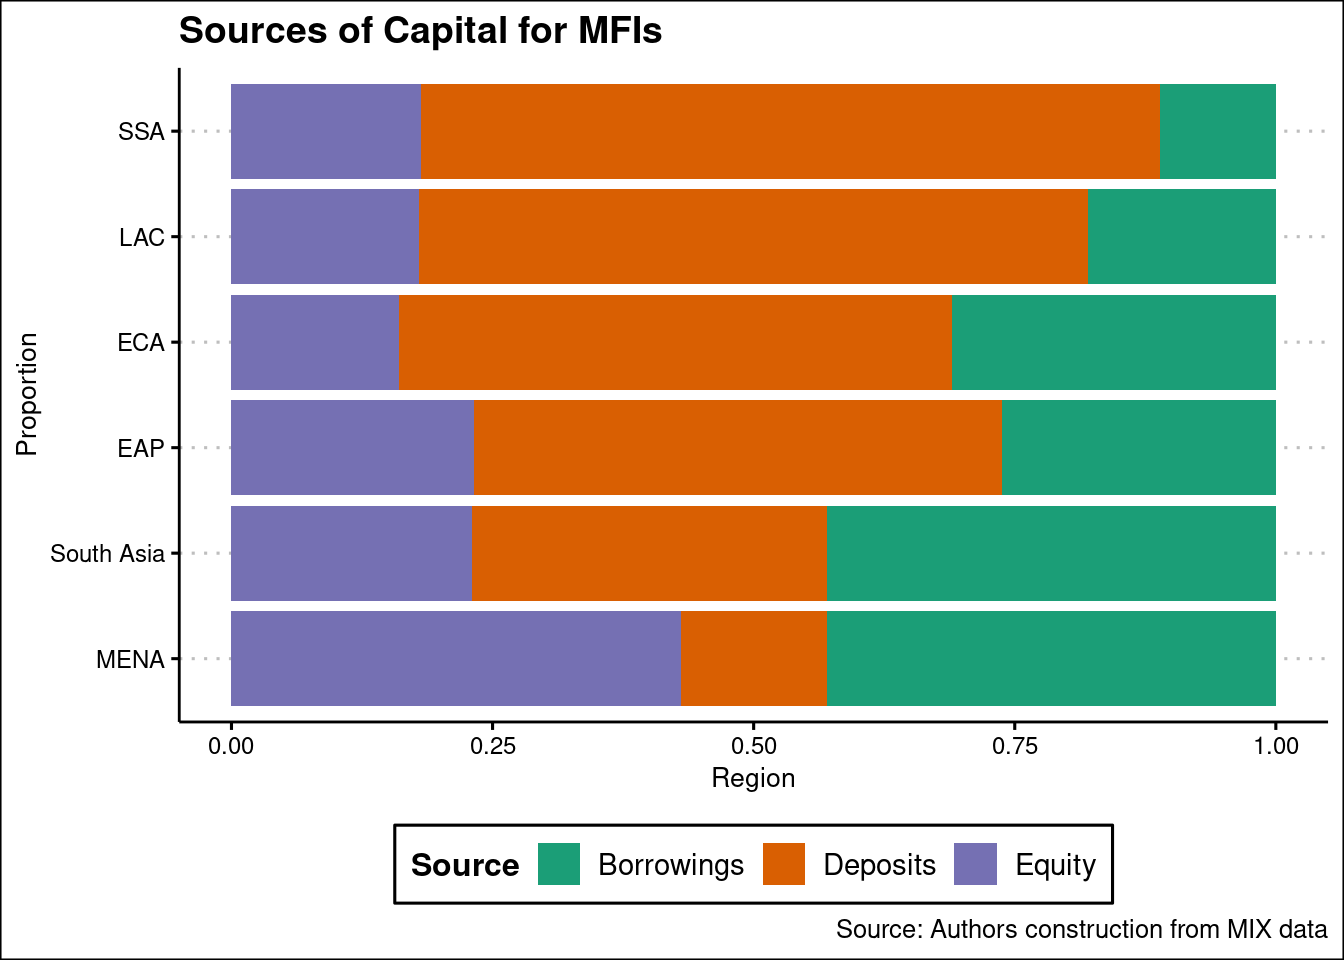
\includegraphics{_main_files/figure-latex/unnamed-chunk-5-1.pdf}
\caption{\label{fig:unnamed-chunk-5}Funding structure of MFIs Across the Globe by Region (2015)}
\end{figure}

Although the transformation of NGOs has its merits, most MFIs have still not transformed\autocite{d2017ngos}. Therefore, the key outputs of this study are the motives behind some MFIs transforming while other MFIs retain the NGO model. The current literature has been overly concerned with the transformed MFIs and has not addressed this issue. Even among the transformed MFIs, researchers have not uncovered the drivers of the decision by MFIs to change and the necessary preconditions for transformation. The existing research takes for granted that MFIs transform to be sustainable. Given the benefits of transformation touted in the numerous studies, then most MFIs should have already converted.

Moreover, as \textcite{morduch2019challenges} argues, if there is no trade-off between financial performance and social performance of transformed MFIs, NGOs would not exist. However, this is not the case. Therefore, it appears that some additional factors influence the decision by MFI to either transform or retain the NGO model. As noted, there is no conclusive evidence on the effects of MFI transformation on their performance. These contradicting results could be because of numerous unknown reasons. It is in order, therefore, to establish the factors that influence the sustainability and outreach of transformed MFIs. Similarly, establishing the factors that moderate the relationship between capital structure on the one hand and the financial performance and social performance of MFIs in Africa is a novel contribution to the research.

Recent literature also suggests that the performance of MFIs is dependent on the broader macroeconomic conditions as well \textcite{ahlin2011does}, and is country-specific \autocite{d2017ngos}. Thus, in the analysis of the institutional transformation of MFIs, cross-country and regional differences must be factored in. However, most studies have not considered the cross country and regional variations. Failure to consider regional disparities means that the extant research fails to capture local contextual peculiarities.

These regional differences motivate the choice of MFIs in Africa as the unit of analysis. By focusing on Africa, the study isolates the regional and country heterogeneity of the effects of transformation. This issue could have affected the results of research based on pooled global datasets. Thus, the output of the study are unique to Africa and therefore more actionable. To sum up this section, the study significantly extends the existing literature on MFI transformation. The following section outlines the purpose statement.

\hypertarget{purpose-statement}{%
\section{Purpose Statement}\label{purpose-statement}}

\noindent This research evaluates the transformation of MFIs in Africa and how this transformation impacts the financial and social performance of MFIs and financial inclusion on the continent.

\hypertarget{research-questions}{%
\section{Research Questions}\label{research-questions}}

\noindent The study specifically seeks answers to the following research questions.

\begin{enumerate}
\def\labelenumi{\arabic{enumi}.}
\tightlist
\item
  Why do some MFIs in Africa transform into the commercial model while others retain the NGO Model?
\item
  To what extent has the institutional transformation of MFIs in Africa affected financial inclusion?
\item
  After transformation, what factors explain the joint level of sustainability and outreach by MFIs in Africa?
\item
  What are the drivers of financial efficiency, social efficiency and socio-financial efficiency of MFIs in Africa?
\item
  What are the factors that influence the choice of financing sources by transformed MFIs in Africa?
\end{enumerate}

\hypertarget{significance-of-the-study}{%
\section{Significance of the Study}\label{significance-of-the-study}}

\noindent In pursuing the stated objectives, this study fills a theoretical deficiency in the capital structure of quasi-commercial organisations that have a social dimension of value. The context of shareholder and debt holder importance was the foundation of capital structure and agency theories. Arguments from this genesis have not factored in corporations with extra dimensions of value, such as achieving social goals. As a case in point, \texttt{Modigliani\ and\ Miller} capital structure theory may not be entirely applicable to MFIs where value also has a social facet. In the Modigliani and Miller capital structure theory, the value of a firm is the sum of equity and debt components in the capital structure of a corporation. The value of a company is an increasing function of the debt proportion of capital structure up to the point where the costs of financial distress outweigh the benefits of the interest tax shield. The empirical output has implications on policy direction relating to MFIs in Africa.

The study also has a variety of policy implications. These policy implications are related to the research objectives. For instance, what are the factors that drive MFIs to transform or fail to transform? The answer to this question would inform the crafting of supportive policies if transformation is indeed desirable. Similarly, uncovering the drivers of financial inclusion, outreach, and sustainability of MFIs after the conversion would inform policy-making supporting financial inclusion. Establishing the determinants of financing sources would allow policy-making to ease fundraising by MFIs. If the drive for institutional transformation is to achieve the desired effects, then the change in the MFI funding structures must not compromise social objectives. If the conversion of MFIs negatively affects social performance, there would be no way to justify the transformation of MFIs. The change of MFIs should improve their sustainability, but not to the detriment of social performance.

Also, if the transition results in a decline in social performance, then the transformation could be treated as the transition point of transformed MFIs into the mainstream banking system \autocite{kent2013bankers}. Therefore, it is crucial to investigate the outcomes of the change to inform the design of a framework that would not expose the poor and financially excluded to the same level of exclusion by the financial system that MFIs ought to address. Doing this would be equivalent to allowing MFIs to use the underprivileged as a ladder to climb into the mainstream system and abandoning them shortly after, which raises ethical questions. Similarly, identifying factors that influence the choice of financing structures has implications for the design of policies aimed at the capital market. For the same reasons, identifying factors that influence the social performance of transformed MFIs is also helpful, not just for policy design but also for managerial decision making.

Finally, the efficiency of MFIs is a significant determinant of both the financial and social performance of MFIs. According to the efficiency theory, the positive relationship between concentration and profitability is indicative of the tendency of firms that are efficient to be successful and hence dominant in their industries \autocite{lipczynski2005industrial}. Efficiency gains could result from economies of scale and cost-saving schemes initiated by the management. Enhanced efficiency by MFIs is, therefore, desirable. However, the efficiency of MFIs should encompass both financial and social dimensions. The entry of commercial sources of capital may affect both the financial and social efficiency of MFIs in line with agency theory. Therefore, it is vital to establish the relationship between capital structure and efficiency to inform both the management and stakeholders of the dynamics in the MFI sector regarding effectiveness in the new era of commercial funding.

\hypertarget{key-findings-of-the-research}{%
\section{Key Findings of the Research}\label{key-findings-of-the-research}}

The research examined the transformation of MFIs in Africa. In this section, I summarize the findings for each of the research questions.

\begin{enumerate}
\def\labelenumi{\arabic{enumi}.}
\tightlist
\item
  \emph{Why do some MFIs in Africa transform into the commercial model while others retain the NGO Model?}
\end{enumerate}

In addressing this research question, I applied logit, probit and multinomial logit models to evaluate the factors that drive NGO-type MFIs to convert to commercial profit-oriented MFIs. The results show that at the firm level, age and size influence transformation. Legal tradition, institutional quality, and stock market development are significant factors at the country level. Specifically, larger and older MFIs are less likely to be NGOs. These results suggest that as MFIs mature, they tend to convert to the commercial model either due to pressure from donors or the decision by management to pursue the double bottom line as they get more financially sustainable and as donor support subsides. MFIs in civil law countries are also less likely to be NGOs, while those in countries that follow other legal traditions are more likely to adopt the commercial model. Again, Institutional quality raises the chances of MFI conversion to the commercial model. Institutional quality captures a wide range of governance measures that enhance contract enforcement and property rights. Hence, countries with stronger institutions tend to attract more private investments and hence the higher rate at which MFIs adopt the commercial model. Stock market capitalisation and private credit to GDP have a negative relationship with transformation. The development of capital markets corresponds to better access to financial services, a pre-condition for financial inclusion. Hence, MFIs in countries with well-developed financial markets will likely be competing against established financial intermediaries for the existing market. The competition limits the financial viability of MFIs. Hence, MFIs in these markets will likely remain NGOs that serve small population in the fringes of the market.

\begin{enumerate}
\def\labelenumi{\arabic{enumi}.}
\setcounter{enumi}{1}
\tightlist
\item
  \emph{To what extent has the institutional transformation of MFIs in Africa affected financial inclusion?}
\end{enumerate}

In this analysis, I used the fixed effects and random effects models to examine how the transformation of microfinance institutions to the profit-oriented model has affected financial inclusion in Africa. I used three indicators of financial inclusion. To the proxy depth of MFI outreach, I used the per cent of female borrowers and average loan balance per borrower. Gross loans to total assets proxied the breadth of outreach. The primary independent variable was the legal form of MFIs: NGOs, NBFIs, commercial banks, cooperatives and rural banks. The control variables were age, region, operating expense to assets ratio, donations to assets ratio, capital to assets ratio, asset structure, MFI size (logarithm of assets), education and profit margin. Our results show that the change from the NGO model to the commercial models could negatively affect the depth of financial outreach, especially given that NGOs characteristically have better outreach to women and advance smaller denomination loans on average than for-profit MFIs. Also, NGOs have higher median gross loans to assets ratio than other legal forms of MFIs except for credit unions/cooperatives. Overall, the results indicate the potential mission drift, where MFIs that convert to the for-profit model focus more on financial sustainability to the detriment of outreach to the unbanked.

\begin{enumerate}
\def\labelenumi{\arabic{enumi}.}
\setcounter{enumi}{2}
\tightlist
\item
  \emph{What are the drivers of financial efficiency, social efficiency and socio-financial efficiency of MFIs in Africa?}
\end{enumerate}

In this objective, I examined the drivers and levels of financial efficiency, social efficiency, and socio-financial efficiency of microfinance institutions (MFIs) in Africa for 2000-2019. I estimated MFI financial efficiency, social efficiency, and joint financial and social efficiency (socio-efficiency) of MFIs in Africa using the output-oriented Data Envelopment Analysis (DEA). The inputs to the DEA model were equity and liabilities and operating expenses to assets ratio. The social performance outputs in the DEA model were the per cent of female borrowers and the average loan balance per borrower, noting that a lower average loan balance corresponds to deeper outreach. Operational self-sufficiency, a ratio of revenue to operating expenses, was the corresponding financial output measure. I then bootstrapped the efficiency scores. These scores were the dependent variables in the subsequent fixed and random effects regressions. Broadly, our results show a trend of declining financial efficiency by MFIs but no discernible trend in social and socio-financial efficiency. However, NGOs have markedly better social efficiency and socio-financial efficiency scores than other legal forms of MFIs. Surprisingly, only cooperatives and rural banks consistently outperform NGOs financially. The proxies for financial sector development, stock market capitalization to GDP and private credit to GDP, have a negative relationship with social and socio-financial efficiency. Financial efficiency has an inverse relationship with both the size and asset structure of MFIs. These results suggest that the commercialization of MFIs does not necessarily improve their financial sustainability.

\begin{enumerate}
\def\labelenumi{\arabic{enumi}.}
\setcounter{enumi}{3}
\tightlist
\item
  \emph{After transformation, what factors explain the joint level of sustainability and outreach by MFIs in Africa?}
\end{enumerate}

Drawing from the classification matrix by \textcite{chattopadhyay2017applicability} I examined the extent to which MFIs in Africa meet their dual objectives and the factors that drive the attainment of financial and social goals. I captured social goals using the per cent of female borrowers, while the operational self-sufficiency (OSS) captured financial performance. The code zero captured MFIs with a proportion of female borrowers greater or equal to 0.5, and an OSS of at least one. MFIs that did not meet any of these thresholds took a code of one. The other two categories (2 and 3) captured MFIs that achieved one goal and failed in the other. I applied a multinomial logit model. The results show that most MFIs in Africa attain the dual objectives, at 35.88\% compared to 14.76\% that fail in both missions. 23.85\% fail socially but succeed financially, and 25.55\% succeed socially while failing financially. In total, 61.43\% of MFIs attain their social goals. 40.31\% fail financially. However, these results vary across the legal status of an MFI. Rural banks and NGOs are more likely to achieve the dual goals than banks, NBFIs and credit unions. Accordingly, the legal status of an MFI is the most significant driver of the extent of the achievement of the dual goals. NGOs have the highest likelihood of achieving both financial and social goals. This result highlights the risk of mission drift should MFIs convert to the for-profit model. Larger MFIs have a higher chance of meeting financial and social goals. Likewise, larger firms are more likely to succeed socially while failing financially, meaning that larger firms emphasise social impact. Age raises the probability that an MFI will fail financially and socially, as does stock market capitalisation to GDP that proxies capital markets development. Lastly, MFIs in countries following civil law and other legal traditions are more likely to meet at least one of the objectives, unlike MFIs in common law countries.

\begin{enumerate}
\def\labelenumi{\arabic{enumi}.}
\setcounter{enumi}{4}
\tightlist
\item
  \emph{What are the factors that influence the choice of financing sources by transformed MFIs in Africa?}
\end{enumerate}

This research item examined the sources of finance for MFIs in Africa and their associated drivers. The indicators of financing sources were debt-equity ratio (leverage) and capital to assets ratio (equity), deposits to assets ratio (deposits), and donations to assets ratio (donations). We used fixed and random effects models with each of the financing sources as the dependent variables. The significant determinants of financing at the firm level are size, age, legal status, and profitability consistent with theory. For example, asset structure varies inversely with leverage. At the country level, institutional quality (KKM) varies inversely with deposits and donations. Interestingly, coefficients of financial development are not significant across all financial structure proxies, going against stylised facts on the macro-level drivers of firms' financing structure. The results suggest that firm-level factors are more relevant in determining the financing structure of MFIs.

\hypertarget{outline-of-the-study}{%
\section{Outline of the Study}\label{outline-of-the-study}}

\noindent The remainder of the work is organised into five standalone chapters of coherent, identifiable aspects of the economics of microfinance in the African context. The proceeding paragraphs highlights each of the chapters.

\textbf{Chapter Two}: This chapter explores the factors behind the transformation of MFIs in Africa from NGOs to commercial, profit-seeking entities that rely more on commercial rather than donor funding. Much of the extant research has looked into the potential effects of the transformation. However, few seek the answer as to why MFIs choose or abstain from converting in the first place. The answer to this question would benefit policy makers in dealing with sustainable financial inclusion in Africa and beyond. The analysis rests on the institutional theory of the causes of change in organizations \autocite{scott2005institutional,powell2012new}, noting that MFIs have been under increasing pressure to be financially sustainable \autocite{d2013unsubsidized}.

\textbf{In chapter three}: In this chapter, I examine the way the transformation of MFIs from NGOs to commercial, profit-seeking enterprises has affected financial inclusion in Africa using the fixed and random-effects models. The study draws from the agency and capital structure theories given that transformed MFIs rely less on donations and subsidies and more on capital markets for funding. Commercial funders could push managers to emphasize financial performance at the expense of social goals \autocite{sarma2011ngo}. Considering this, the essay examines how the shift has affected lending to women, average loan sizes and gross loans. The study fills a gap in the literature given that much of the existing literature examines the effects of transformation using global datasets, which could mask regional heterogeneity as \textcite{d2017ngos} suggests.

\textbf{Chapter four}: Chapter four assesses levels of financial efficiency, social efficiency, and joint social and financial efficiency (socio-financial efficiency) of MFIs in Africa. The chapter also evaluates the factors that drive these efficiencies. The analysis is in light of the transformation of MFIs from NGOs to commercial entities where agency conflicts could make MFIs less inclined to avail financial services to the financially excluded in favour of profits \autocite{serrano2014microfinance}. I apply the data envelopment analysis (DEA) approach to quantify the extent that MFIs in Africa translate their assets into financial and social outcomes, which is a novel contribution to financial inclusion in Africa.

\textbf{Chapter five}: Chapter 5 examines the factors that drive the simultaneous achievement of financial and social goals by MFIs in Africa. In this section, I use the multinomial logit model to examine the extent to which MFIs simultaneously achieve both their financial and social goals. I construct the dependent variable using the matrix developed by \textcite{chattopadhyay2017applicability} as described in section 1.8 above. The output from this section complement those in chapter 4 but using a different methodology for robustness.

\textbf{Chapter six}: Chapter 6 examines the funding sources by MFIs in Africa, including the factors determining the sources of financing. The mainstream capital structure theory does not address hybrid organisations with a dual mission, such as MFIs. The results would be useful at informing decisions about financing alternatives for MFIs that would best suit their hybrid nature, more so to meet their social goals while remaining financially sustainable.

\textbf{Conclusion}: Finally, the study concludes by summarising findings, offering policy recommendations, and pointing out possible directions for future research.

\begin{savequote}
``All is changed, save the river and the hill-- Even they are changed.
Only the burning sun and the quiet stars are the same. And we--we, the
memories, stand here in awe, Our eyes closed with the weariness of
tears-- In immeasurable weariness.''
\qauthor{--- Edgar Lee Masters.}\end{savequote}



\hypertarget{cites-and-refs}{%
\chapter{Transformation of Microfinance Institutions in Africa}\label{cites-and-refs}}

\chaptermark{Transformation of MFIs in Africa}

\minitoc 

\begin{center}

\textbf{ABSTRACT}

\end{center}

We examine the factors that drive non-governmental organisation type of microfinance institutions to convert to the commercial, profit-oriented model. Using data from the World Bank and the International Monetary Fund (IMF), we ran logit, probit, and multinomial logit regressions, with NGOs as the base outcome. At the firm level, age and size influence transformation, whereas legal tradition, institutional quality, and stock market development are significant factors at the country level. More specifically, older firms are less likely to be NGOs, as are MFIs in civil law countries. Larger MFIs and MFIs located in countries with ``other'' legal traditions are more likely to follow the commercial model. We also found that institutional quality increases the likelihood of conversion, while stock market size has a negative relationship with transformation. These models are statistically significant, and their associated results remain robust to removing outliers and other checks.

\vspace{10mm}

\textbf{Key Words}: Microfinance, Transformation, NGO, Commercial, Africa.

\vspace{5mm}

\textbf{JEL Classification}: G210, G230

\newpage

\hypertarget{background}{%
\section{Background}\label{background}}

The modern micro-finance (MF) industry draws its popularity from the promise of providing appropriate and affordable financial services to the population under-served by mainstream financial intermediaries \autocite{morduch1999microfinance,morduch2000microfinance}. The motivation for reaching out to the unbanked draws from researchers and development practitioners' view that financial inclusion leads to welfare improvements. As an example, some scholars associate access to finance with more business start-ups, higher savings rates, improved health, less child mortality, and higher education attainment by the poor, although some scholars downplay these findings \autocite{klapper2015role,o2017systematic,shahriar2017lender}. Much of the initial efforts to provide financial services to the unbanked rested on Microfinance. Microfinance refers to either the practice of delivering appropriate and affordable financial facilities to the financially excluded or the providers of such micro and small denomination financial services \autocite{ledgerwood2006transforming} \footnote{The quote at the beginning of the chapter is from the poem \emph{Edith Conant} by Edgar Lee Masters in \textcite{masters2007spoon}}.

Pioneer Microfinance Institutions (MFIs), like Grameen Bank, primarily operated as Non-Governmental Organisations (NGOs), following the welfare approach, where the profitability of the institution played a second role to availing financial services to the poor \autocite{chahine2010social,d2017ngos}. However, the paradigm shift is towards the financial systems approach where MFIs operate under commercial principles, leading to charges of ``financialisation'' of poverty \autocite{mader2015financialization}, with the relatively higher interest rates charged to the clients equated to a ``poverty penalty'' \autocite{chen2017microfinance}. Some scholars and practitioners argue that MFIs following the profit-oriented commercial model are subject to ``mission drift'' though more financially sustainable''. Mission drift refers to situations where MFIs lessens their commitment to availing financial services to the financially excluded to pursue profits \autocite{jia2016commercialization,mia2017mission}.

However, given the social mission inherent in MF, MFIs following the financial systems approach risk their legitimacy in society and local and international donor community, a significant source of funding even for commercial MFIs \autocite{nason2018behavioral}. For these reasons, some researchers and development practitioners vouch for the welfare approach, where MFIs focus primarily on the mission to reach the financially excluded without emphasising profits. Most MFIs following the welfare approach are non-governmental organisations (NGOs). Though not subject to mission drift, the NGO model is over-reliant on volatile local and international donor funds and government subsidies \autocite{garmaise2013cheap,d2017aid}. Additionally, NGOs may crowd out the efficient, commercial-oriented microfinance providers \autocite{kota2007microfinance}, which may hurt aggregate welfare in the long run.

The win-win school attempts to reconcile the commercial model and welfare approach to microfinance. Adherents of the win-win school postulate that it is possible to achieve both financial sustainability (that is, turn a profit) and, at the same time, reach the financially excluded \autocite{kodongo2013individual}. As a case in point, some researchers argue that MFIs could strive to generate profits by offering financial services to the relatively well-off at market rates. The MFIs could then use the returns to subsidise the provision of financial services to the poor under a form of price discrimination, leading to ``mission expansion'' as opposed to mission drift \autocite{mersland2010microfinance}.

Globally, the shift from the pure welfare approach of MF provision is gaining ground. Most of the transformed MFIs operate at some point on the continuum between the NGO, welfare model and the commercial, profit-oriented approach \autocite{armendariz2013subsidy,d2013unsubsidized,hishigsuren2006transformation}. It all started in 1992 in Bolivia when Prodem, an NGO, converted to a commercial bank, Bancosol \autocite{fernando2004micro,creedy2018types}. Since then, many MFIs worldwide have converted from NGOs to commercial firms seeking to make profits.

This article explores the factors that drive the transformation of MFIs from NGOs to for-profit firms in Africa. To this end, we use a panel dataset of 705 MFIs in Africa from the MIX pooled database, with additional data from the World Bank like the World Development Indicators (WDI), the Worldwide Governance Index (WGI), and the Global Financial Development Database (GFDD). We focus on Africa, given the relatively low levels of financial inclusion on the continent \autocite{demirguc2018global}and the shortcomings inherent in combining data from different regions that may yield results that are not actionable. As \textcite{d2017ngos} and \textcite{wang2015ownership} suggest, the nature and performance of MFIs are country-specific. Hence, research focusing on particular regions, countries or even firms could better inform policymaking.

This article contributes to the literature in two main ways. First, the study sheds light on the drivers of the transformation of microfinance institutions in Africa. Much of the literature has not examined this phenomenon, focusing, instead, on the shift's consequences and how MFIs can balance financial and social missions \autocite{d2013unsubsidized,forkusam2014does,mia2017mission}. We believe that our analysis could form a reasonable starting point for analysing the transformation of MFIs in other regions or countries. Second, we detail the linkages between the drivers of micro-finance institutions' transformation, showing how they interact to change the likelihood of conversion. We highlight the pitfalls that bedevil analysis of pooled data from heterogeneous sources, which may mask crucial differences or similarities between the analysis units.

The rest of the article is structured as follows. Section 2.3 presents the theoretical underpinnings and empirical findings related to the study. Subsequently, in section 2.3.1, we summarise the findings of this study before delving into the analysis method and attendant results in sections 2.4 and 2.5, respectively. Section 2.6 concludes.

\hypertarget{related-literature}{%
\section{Related Literature}\label{related-literature}}

Much of the early literature on the institutional change of MFIs dealt with the theoretical, philosophical, and historical basis for transforming MFIs from NGOs to commercial firms and the potential impacts of such conversion \autocite{campion1999institutional,christen2001commercialization,gutierrez201920,zaby2019science}. Views of scholars on the transformation of MFIs drew from the institutional theory. The theory seeks to explain persistence and convergence in organisations, including change and de-institutionalisation within firms \autocite{scott2004institutional}. For MFIs, the transformation has picked pace with the dominance of neoliberalism after the cold war \autocite{ostry2017}.

The institutional theory holds that the institutional environment is more influential in developing formal structures in organisations than market pressures \autocite{maggio1991}. Coercion is one form of pressure from the institutional environment that makes organisations adopt institutional structures and practices. Institutional theorists note that stakeholders could force firms to adopt specific organisational structures and practices without critical scrutiny to gain legitimacy in the institutional environment \autocite{scott2004institutional,martinez2017coercive}.

With this hindsight, \textcite{bateman2010doesn} traces the pressure to convert MFIs from NGOs to the commercial model to the rise of neo-liberalism and the insistence that firms be financially self-sufficient instead of relying on government subsidies and, in the case of MFIs, donor funds. The wave of economic liberalisation and privatisation commenced in the early 1990s due to neo-liberalism \autocite{silva1998neoliberalism}. Researchers point to pressure from financiers of MF such as USAID and the World Bank as a significant driver for the decision for MFIs to transform \autocite{ostry2017}.

However, given that MFIs have a social mission, the transition to a profit-oriented positioning is bound to conflict with the social objectives and threaten the MF industry's legitimacy \autocite{ramus2017,nason2018behavioral}. Specifically, the quest to satisfy both financial goals and the social mission is likely to conflict, which may cause ``mission drift'' \autocite{mersland2010microfinance,mia2017mission}, where MFIs give greater priority to profitability than outreach to the unbanked.

Nonetheless, the push from donors to transform MFIs seems to contradict the slow pace of the transformation. NGOs still form a substantial proportion of MFIs in Africa, accounting for 32\%, second only to Non-Bank Financial Institutions (NBFIs) at 40\% \autocite{market2017global}. A question arises regarding the factors behind the persistence of certain organisational forms of MFI provision in Africa and globally. \textcite{pashkova2016business} tackled this question. They found that the cooperative model is prevalent in economies with civil law systems, low inflation levels, and high economic growth rates.

In contrast, NGO type MFIs feature in countries with high inflation rates and low economic growth levels, meaning that NGOs help the poor cope during challenging economic times. The commercial banking model features most in economies with common law legal systems. However, the study by Pashkova, et al.~does not explicitly address the transformation question, factors that determine the transformation of MFIs from NGOs to a commercial model, which we explicitly address in this article.

The capacity of the capital markets and their antecedents may raise the propensity for the transformation of MFIs. MFIs in countries with well-developed capital markets can efficiently or more readily issue debt and equity instruments and raise public deposits \autocite{allen2013resolving,allen2014african}. Available literature points to legal tradition, governance, and education, as drivers of financial development in a country \autocite{rajan1998financial,baltagi2009financial}. By extension, these variables drive economic growth by the financial development-economic growth nexus literature \autocite{claessens2003financial}. The size of an MFI in terms of assets base, structure, and tangibility could enhance its capital acquisition capacity in line with the trade-off theory of capital structure \autocite{barclay2005capital,gwatidzo2009corporate,ojah2016effects}.

\textcite{ledgerwood2006transforming} attribute the financing structure, hence the organisational form of an MFI, to the institutional life cycle. For instance, in the early stages, most MFIs operate as NGOs relying on donations and concessionary funds, given that commercial funders deem them too risky. Later, they use government subsidies and equity funding from NGOs and public investors to supplement their funding. In the final consolidation phase, most MFIs rely on debt, using foreign donors as guarantees. Deposits also play a prominent role in this consolidation phase as MFIs increasingly adopt the commercial model.

Thus, the age of an MFI may have a bearing on both the capital structure and organisational structure. Regulatory provisions relating to the ways MFIs can raise capital and historical legacies on saving and lending \autocite{bayai2016financing} may explain the remaining firm, country and regional disparities. The agency conflict that follows the introduction of debt and equity brings to the fore the potential conflict between optimising financial returns and sticking to the social mission of MFIs, the second central strand of research on MFI conversion \autocite{nurmakhanova2015trade,bayai2016financing,abdulai2017trade,awaworyi2018sustainability}.

Quality of institutions features prominently in explaining the investment climate in a country. Researchers have primarily explained away the ``Lucas Paradox'' using the differences in, among others, the institutions, especially the capacity to enter into and enforce contracts and guarantees against state appropriation of private property - property rights \autocite{azemar2013has,goktan2015explanation}. MFI transformation connotes the entry of private, profit-oriented capital that seeks returns and favours countries with refined institutions. Moreover, researchers have variously cited the quality of institutions as drivers of the ease with which firms, MFIs included, can access private funds by fostering a well developed financial ecosystem \autocite{huang2010political,kaidi2019financial}. In this case, the financial system would consist of equity and debt markets where private investors could buy stakes in or lend funds to the MFIs that seek to go commercial. The following section highlights the results of the study.

\hypertarget{summary-of-results}{%
\subsection{Summary of Results}\label{summary-of-results}}

The output from the data analysis shows that at the country level, it is legal tradition, stock markets development, and governance (institutional quality) that relate significantly to the likelihood of the transformation of MFIs. At the firm level, the age and size of the MFI raise the probability of conversion. There is also a robust time trend towards the commercialisation of MFIs which points to the growing acceptance of microfinance's profit orientation. Regional differences are also evident with North Africa represented by NGOs in the sample data, probably due to religious constraints. GDP growth rate and education levels are not significant determinants of the probability of transformation. However, like the stock market to GDP, private credit to GDP has a negative coefficient, suggesting sensibly that the availability of larger financial markets does not support MFIs' model conversion.

Precisely, the probability of an MFI transforming declines with the increase in age, with older MFIs more likely to follow the NGO model than younger MFIs. In contrast, bigger MFIs have a higher likelihood of transforming to the commercial model, while smaller MFIs retain the NGO status. Also, MFIs in common law countries have a higher chance of changing than civil law countries. However, MFIs located in countries with other legal traditions (that is, not civil or common law traditions - see Appendix 6) that have the highest probability of going commercial. Stock market development relates negatively with the likelihood of transformation of MFIs, likely because people in countries with well developed financial markets are more likely served by the mainstream financial system, relying less on microfinance. However, only stock market development is a significant driver of the financial development indicators, with private credit having a negative but insignificant effect of transformation. As expected, governance/ institutional quality positively relates to the chance of a conversion. Regionally, the sample data has only NGOs for North Africa, reflecting religious aversion to for-profit microfinance operating in majority Muslim countries. Importantly, there is a potent time trend towards the commercialisation of MFIs which points to a triumph of the commercial approach to microfinance over the welfare model. GDP growth rate shows mixed results but is insignificant. In the next section, we describe the methodology applied in the study.

\hypertarget{method}{%
\section{Method}\label{method}}

The article uses three empirical estimation approaches, the binary logit and probit models and the multinomial logit model, given that our dependent variable is discrete and error terms may not be normally distributed \autocite{cramer2002origins}. For the logit and probit models, MFIs following the NGO model take a code of zero and NBFIs, credit unions/ cooperatives, and rural banks forms taking a code of one. NGOs still take a zero-code for the multinomial logit model, with commercial banks, NBFIs, credit unions, and Rural Banks taking codes of one, two, three, and four, respectively. The multinomial logit model will help uncover factors that drive the choice of a particular legal form by NGOs adopting the commercial model. NGOs converting to the commercial model can turn to commercial banks, credit unions, NBFIs, or rural banks. The following section lays out and describes the models, variables, and data sources.

\hypertarget{the-model-variables-description-and-data-sources}{%
\subsection{The Model, Variables Description and Data Sources}\label{the-model-variables-description-and-data-sources}}

We use the model below to run both logit and probit regressions on a panel dataset of 705 MFIs in Africa. Assuming the error term \(\epsilon\) follows a logistic distribution \autocite{czepiel2002maximum}, we have,

\begin{equation}
y_{it} = log(\frac{p_{it}}{(1-p_{it})} ) = \alpha + x_{it} + \varepsilon_{it}
\end{equation}

where,

\begin{equation}
p_{it}  =  \frac{1}{1 +  e^{- z_{it} } } 
\end{equation}

and

\begin{equation}
1 + p_{it}  =  \frac{1}{1 +  e^{z_{it} } }, for z_{it} = f(x_{it})
\end{equation}

In the model, \(y_{it}\) is the current legal status of the MFI, the dependent variable which is a dummy with zero, representing NGOs as the base outcome. The other legal forms of MFIs take a code of one. The symbol \(x_{it}\) represents a vector of independent variables: age, size, capital market development, legal tradition, GDP growth rate, and institutional quality. Additionally, we include year dummies to cater for the trends towards commercialisation.

The multinomial logit model extends the binary logit model to more than two unordered levels (discrete choices). The data at hand meets the requirements for running a multinomial logit model as the dependent variable (the legal status of each MFI) has one outcome for each case. Also, the independent variables do not faultlessly predict the dependent variable \autocite{petrucci2009primer}. Suppose we have a dependent variable \(y\) consisting of \(K\) choices for \(K>=2\). Further, let the independent variables be \(x_1, x_2,………. x_n\), we can specify the multinomial logit model as follows.

\begin{equation}
log(\frac{prob(k/X)}{prob(K/X)}) =   \beta_{0}^{k}  x_{0}  + \beta_{1}^{k}  x_{1} +  \cdots + \beta_{p}^{k}  x_{p}, for k = 1 \cdots K-1
\end{equation}

\(y\) is the dependent variable, in this case, one of NGO, commercial bank, NBFI, credit union or rural bank and \(x\) is a vector of independent variables.

If \(K>2\), then we have a multinomial logit with \(K-1\) set of equations. Where \(K=2\), the model is the binary logit model denoted in equation one (1) where we have one equation. Note that we have arbitrarily assigned the last category (K) as the reference in this case. Any other group can serve as a reference and hence not be part of the equations set.

One of the significant drawbacks of the multinomial logit is the violation of the assumption of the independence of irrelevant alternatives (IIA). \textcite{cheng2007testing} ) illustrate this assumption using the blue bus- red bus example. If the choice between car transport and a red bus, and given that the probability of choosing a bus is \(0.8\), and \(0.2\) for a car, then the bus's odds over car transport is 4. Suppose we introduce a third alternative, the blue bus. If the probabilities of choosing a red bus, blue bus, and car transport are \(0.6\), \(0.25\), \(0.15\), respectively, the assumption holds since the odds of selecting a red bus over a car are still \(4\). If the odds are different from \(4\), then the model violates the IIA, and the multinomial model is not fit for the data. In our case, we plausibly see the assumption holding because the legal status of an individual MFI is independent of the legal status of other MFIs. Table 2.1 (next page) describes the variables in detail.

\begin{table}

\caption{\label{tab:unnamed-chunk-13}Description of Variables}
\centering
\fontsize{9}{11}\selectfont
\begin{tabu} to \linewidth {>{\raggedright}X}
\toprule
Variable\_Description\\
\midrule
1. Current Legal Status (Dependent Variable): This is the dependent variable. For logit and probit models, we create a dummy variable with the MFIs following the NGO Model getting a code of zero, and one in the case of non-bank financial institutions (NBFIs), rural banks, and credit unions/ cooperatives. We assign codes of zero to four for the multinomial logit model for NGOs, Banks, NBFIs, Cooperatives and Rural Banks, respectively. The data are available from the Microfinance Information Exchange, MIX (See source in note 1 below).\\
\\
2.  Age: The period in which the MFI has been in operation. MFIs fall into one of three groups: new (1-4 years), young (4-8 years), and mature (over 8 years). The data are available from MIX.\\
\\
3. Legal Tradition (Legal): The indicator is a dummy variable with common law countries coded 0, civil law countries 1, and 2 otherwise as per the classification by Oto-Peralías and Romero-Ávila (2014). Appendix 6 shows the classification of countries into respective legal traditions\\
\addlinespace
\\
4. Size (Assets): We proxy the size of MFI with the natural logarithm of total assets, again using MIX data.\\
\\
5. Governance/ Institutional Quality (KKM): We take the first principal component of the WGI developed by Daniel Kaufmann, Aart Kraay and Massimo Mastruzzi (KKM) that is available on the World Bank's Worldwide Governance Indicators, WGI (See source in note 3 below).\\
\\
\addlinespace
6. Private Credit to GDP (pcrdbgdp): We capture the total amount of credit advanced to the private sector by financial intermediaries as a proxy for capital markets development concerning the banking sector following Ito and Kawai (2018). The data source is the Global Financial Development Database (GFDD) of the World Bank (See note 4).\\
\\
7. Stock market capitalisation to GDP (stmktcap): We capture the  extent of stock market development using the ratio of stock market capitalisation to GDP to proxy the extent to which firms can raise equity capital. Although Africa's equity markets are thin, some relatively large stock markets like South Africa, Egypt, Nigeria, Kenya, and Ghana exist. The data are from the GFDD.\\
\\
8. GDP annual growth rate (gdp\_growth\_annual): This is the year on year growth in output adjusted for inflation and sourced from the World Development Indicators (WDI) (See note 2).\\
\addlinespace
\\
9. Education (EDUC): The indicator is a ratio of the gross enrolment in secondary school to the gross primary school enrolment as defined in the literature (Allen et al., 2013, 2014). The data are from the WDI.\\
\\
\bottomrule
\multicolumn{1}{l}{\rule{0pt}{1em}Source: Authors' construction from the literature}\\
\multicolumn{1}{l}{\rule{0pt}{1em}\textit{Notes}}\\
\multicolumn{1}{l}{\rule{0pt}{1em}\textsuperscript{1} MIX Database on www.themix.org and https://datacatalog.worldbank.org/dataset/mix-market}\\
\multicolumn{1}{l}{\rule{0pt}{1em}\textsuperscript{2} WDI on https://databank.worldbank.org/source/world-development-indicators.}\\
\multicolumn{1}{l}{\rule{0pt}{1em}\textsuperscript{3} WGI/ KKM on https://databank.worldbank.org/source/worldwide-governance-indicators.}\\
\multicolumn{1}{l}{\rule{0pt}{1em}\textsuperscript{4} GFDD on https://www.worldbank.org/en/publication/gfdr/data/global-financial-development-database}\\
\end{tabu}
\end{table}

\hypertarget{data-analysis-and-results}{%
\section{Data Analysis and Results}\label{data-analysis-and-results}}

\hypertarget{exploratory-data-analysis}{%
\subsection{Exploratory Data Analysis}\label{exploratory-data-analysis}}

In this section, we visualise the data and then describe the variables in the model.

\hypertarget{data-visualisation}{%
\subsubsection{Data visualisation}\label{data-visualisation}}

Figure 2.1 below shows the summary statistics and scatter plots for the independent numeric variables. The summaries show a high correlation between education on the one hand and private bond market capitalisation to GDP, stock market capitalisation to GDP, and private credit to GDP on the other at around 0.5. As literature shows, higher education levels coincide with greater participation of individuals in capital markets as financial inclusion levels rise \autocite{allen2013resolving,allen2014african,ito2018quantity}. The stock market capitalisation to GDP and private bond market capitalisation to GDP correlates vastly, at 0.73. Typically, debt markets mature first, followed by stock markets, and their development levels are highly correlated \autocite{levine1999stock}. Other variables that show a high correlation include private credit to GDP on the one hand and private bond market capitalisation to GDP, and stock market capitalisation to GDP at 0.32 and 0.47. Institutional quality (KKM) also correlates with education, private credit to GDP and private bond market capitalisation \autocite{yartey2008determinants}.

With this hindsight, we drop education and private bond market capitalisation from the model. Note that much of the private credit to GDP ratio's variation already reflects the stock market's GDP ratio. Also, education reflects in general capital market development as documented in the literature \autocite{allen2013resolving,allen2014african}. We also note that North Africa has only NGOs in the model, perhaps due to faith \autocite{allen2013resolving,allen2014african,hassan2018religious}. Hence, we exclude the region in the model. There could be country-specific effects that we capture using the quality of governance (KKM) \autocite{kunvcivc2014institutional} and the annual GDP growth rate \autocite{butkiewicz2006institutional}.

Figure 2.2 shows that mature MFIs dominate the dataset across all legal forms and particularly dominant among rural banks, NGOs, and cooperatives. Turning to the prevalence of MFIs by legal status, cooperatives dominate civil law countries. Simultaneously, NGOs, NBFIs, commercial banks and rural banks dominate common law countries, which researchers have documented \autocite{pashkova2016business}. For other legal traditions, NBFIs and cooperatives dominate. As noted, North Africa has only NGOs in the dataset, which could indicate the religious constraints towards interest charging financial intermediaries \autocite{hassan2018religious}. Finally, while commercial banks and NBFIs show a higher asset base, NGOs and credit unions are not large. Commercial banks assets could be more extensive due to statutory minimum capital requirement resulting from their desire to optimise economies of scale \autocite{aiyar2016does}.

Turning to Figure 2.3, country-level governance matter more for commercial MFIs- commercial banks and NBFIs, compared to NGOs and rural banks in line with the link in the literature between investment, governance, and property rights \autocite{claessens2003financial}. Commercial banks, rural banks, and NGOs dominate countries with higher stock market development levels, while NBFIs and cooperatives trail, noting that cooperatives may be relatively less inclined to obtain funding from stock markets \autocite{porter1987economic}. The result could indicate the importance of equity capital for commercial banks and NGOs, while NBFIs tend to rely more on private equity and debt. Indeed, the data shows NBFIs dominate in countries where private credit to GDP is highest, followed by cooperatives and NGOs, while commercial banks and rural banks come last. Lastly, commercial banks, NBFIs and rural banks tend to dominate countries with higher GDP growth rates. Higher GDP growth implies higher profitability that allows commercial MFIs to thrive. Low GDP growth means that the not-for-profit NGOs and member-oriented cooperatives tend to succeed as a cushion to the vulnerable in society and fill the void left by the commercial MFIs.

\newpage

\begin{landscape}

\begin{figure}
\centering
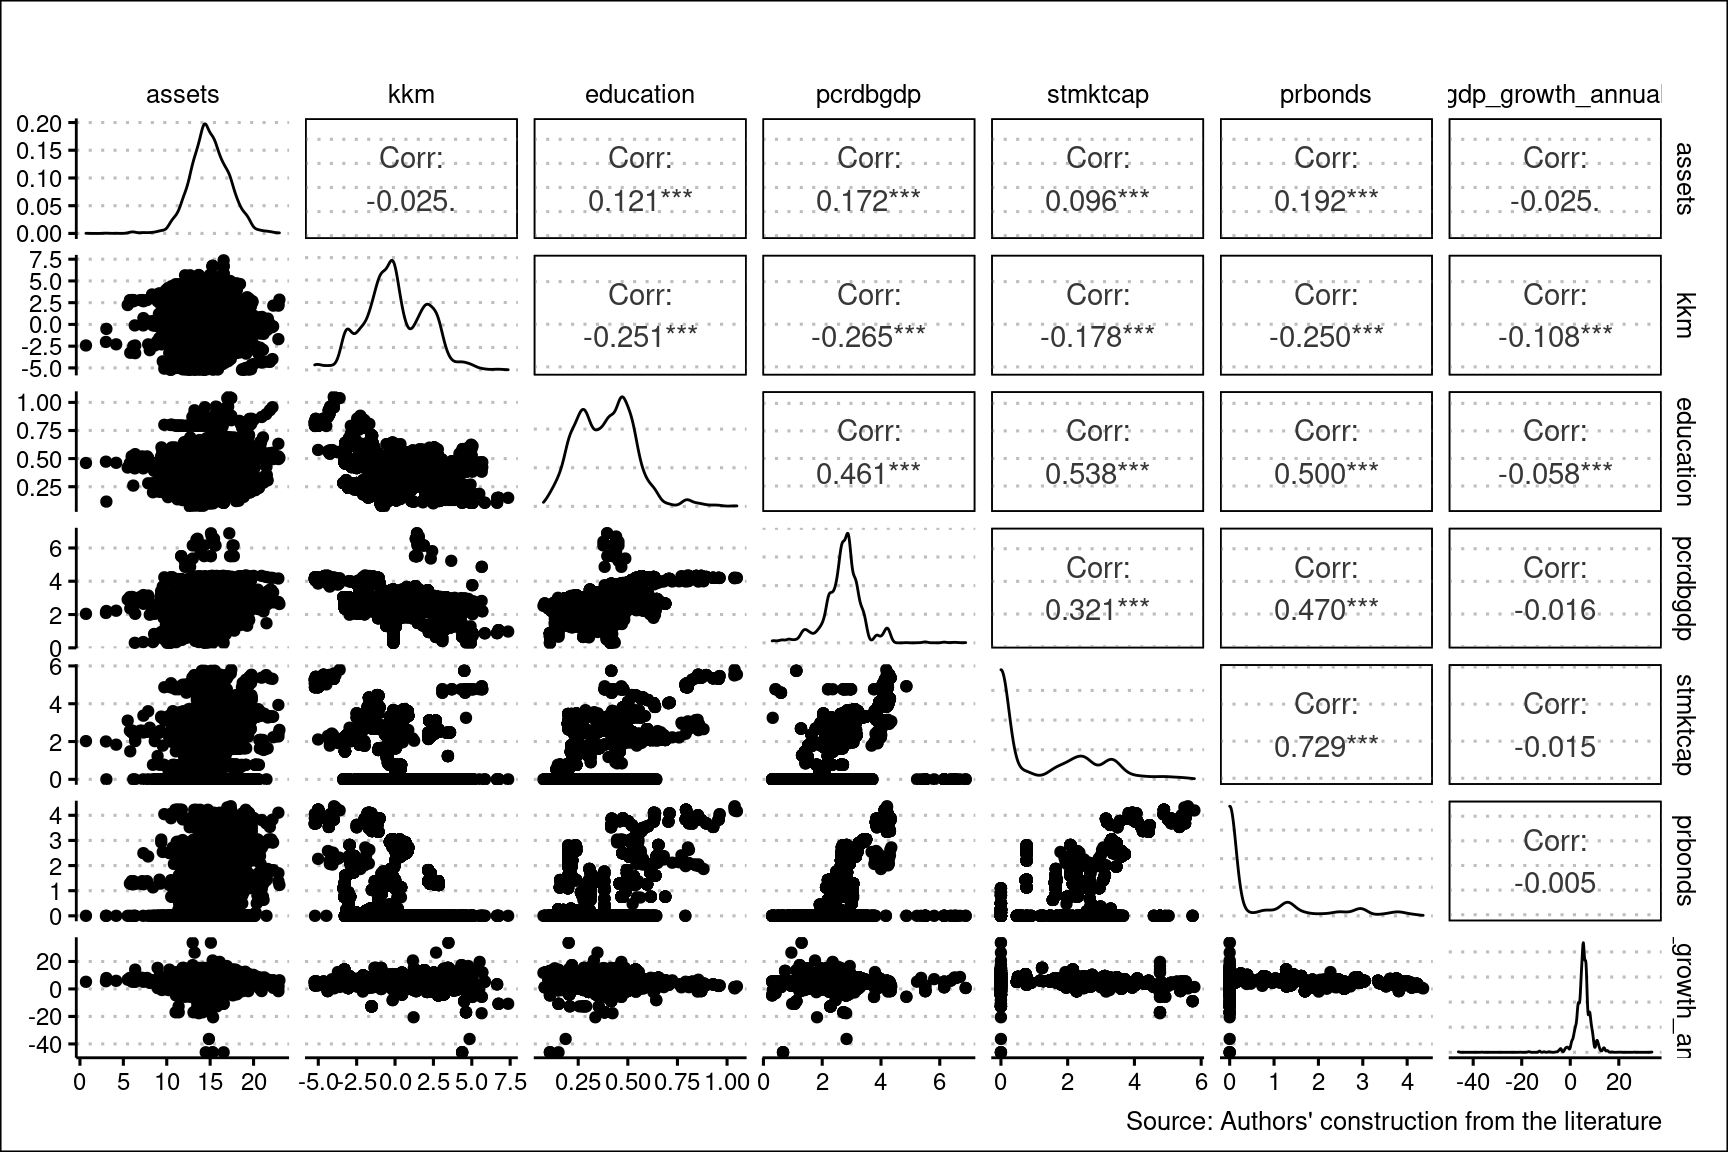
\includegraphics{_main_files/figure-latex/unnamed-chunk-14-1.pdf}
\caption{\label{fig:unnamed-chunk-14}Correlations Between Independent Variables}
\end{figure}

\begin{figure}
\centering
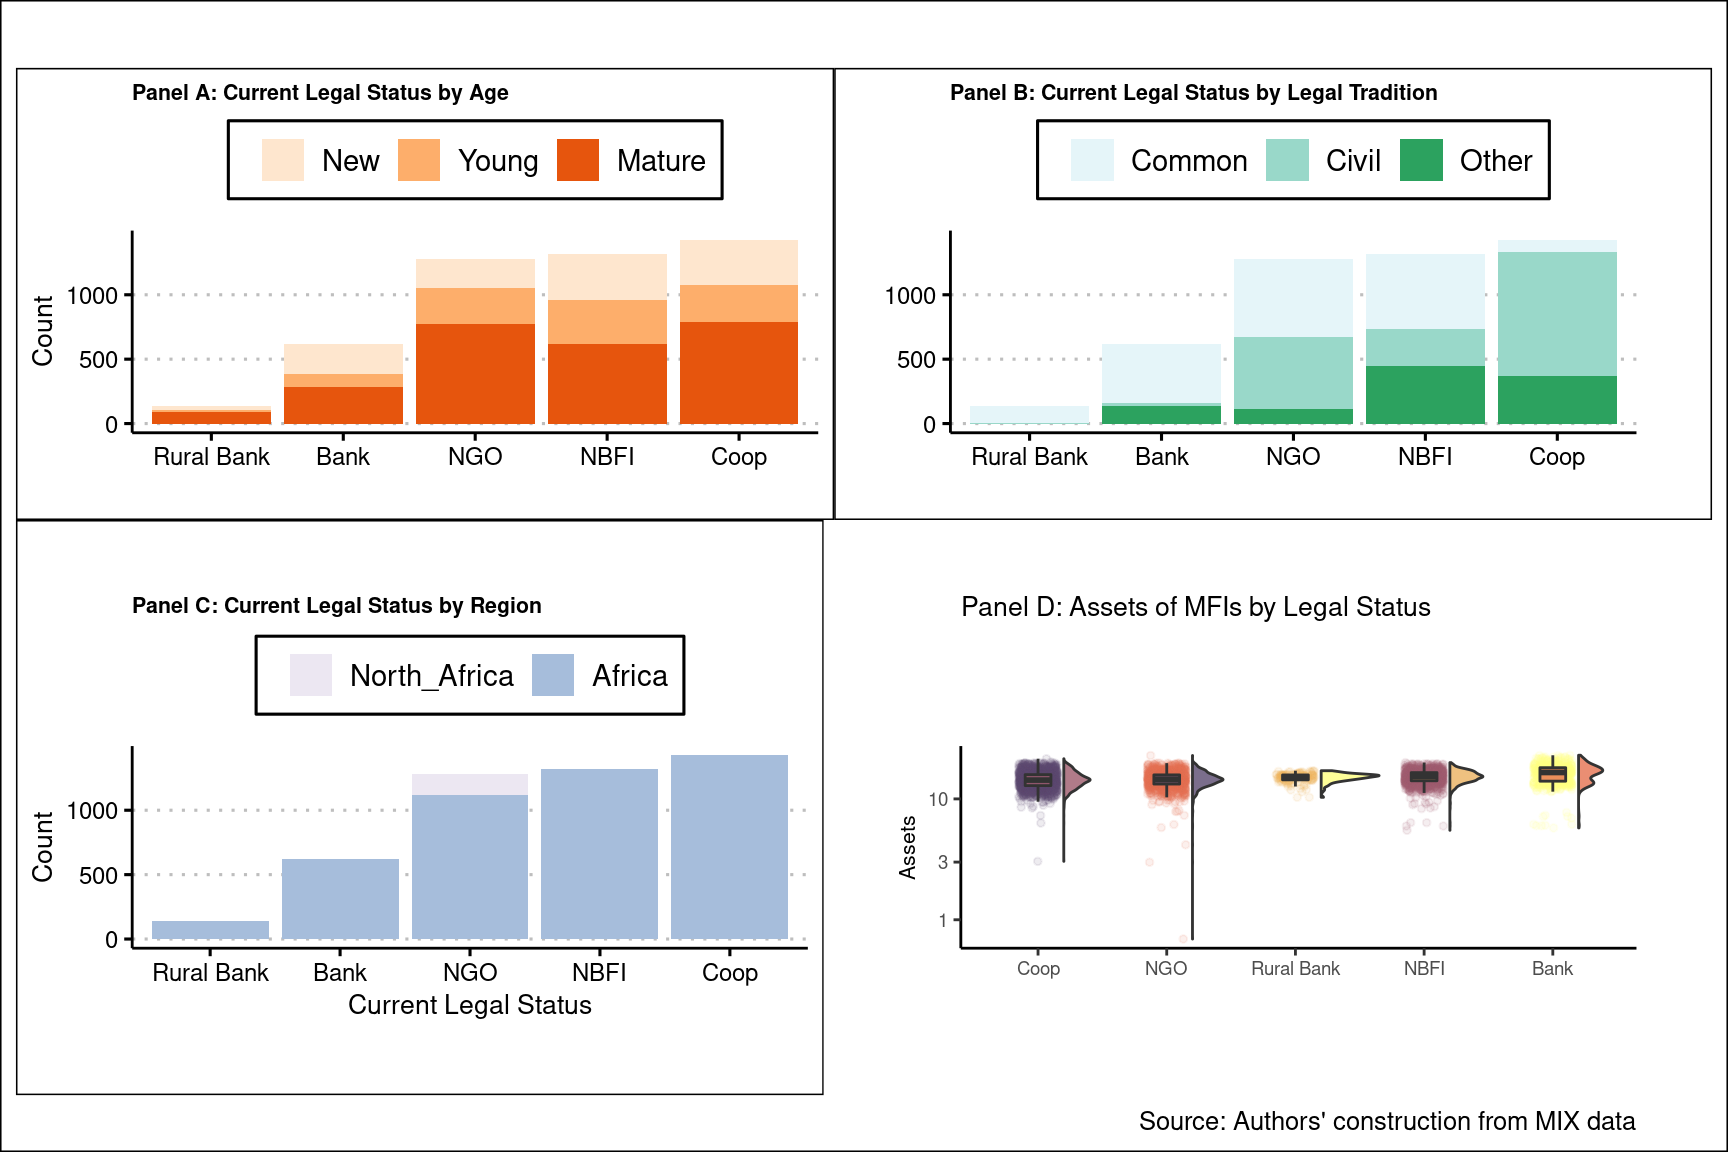
\includegraphics{_main_files/figure-latex/unnamed-chunk-19-1.pdf}
\caption{\label{fig:unnamed-chunk-19}Distribution and Asset Base of MFIs in Africa by Legal Status}
\end{figure}

\begin{figure}
\centering
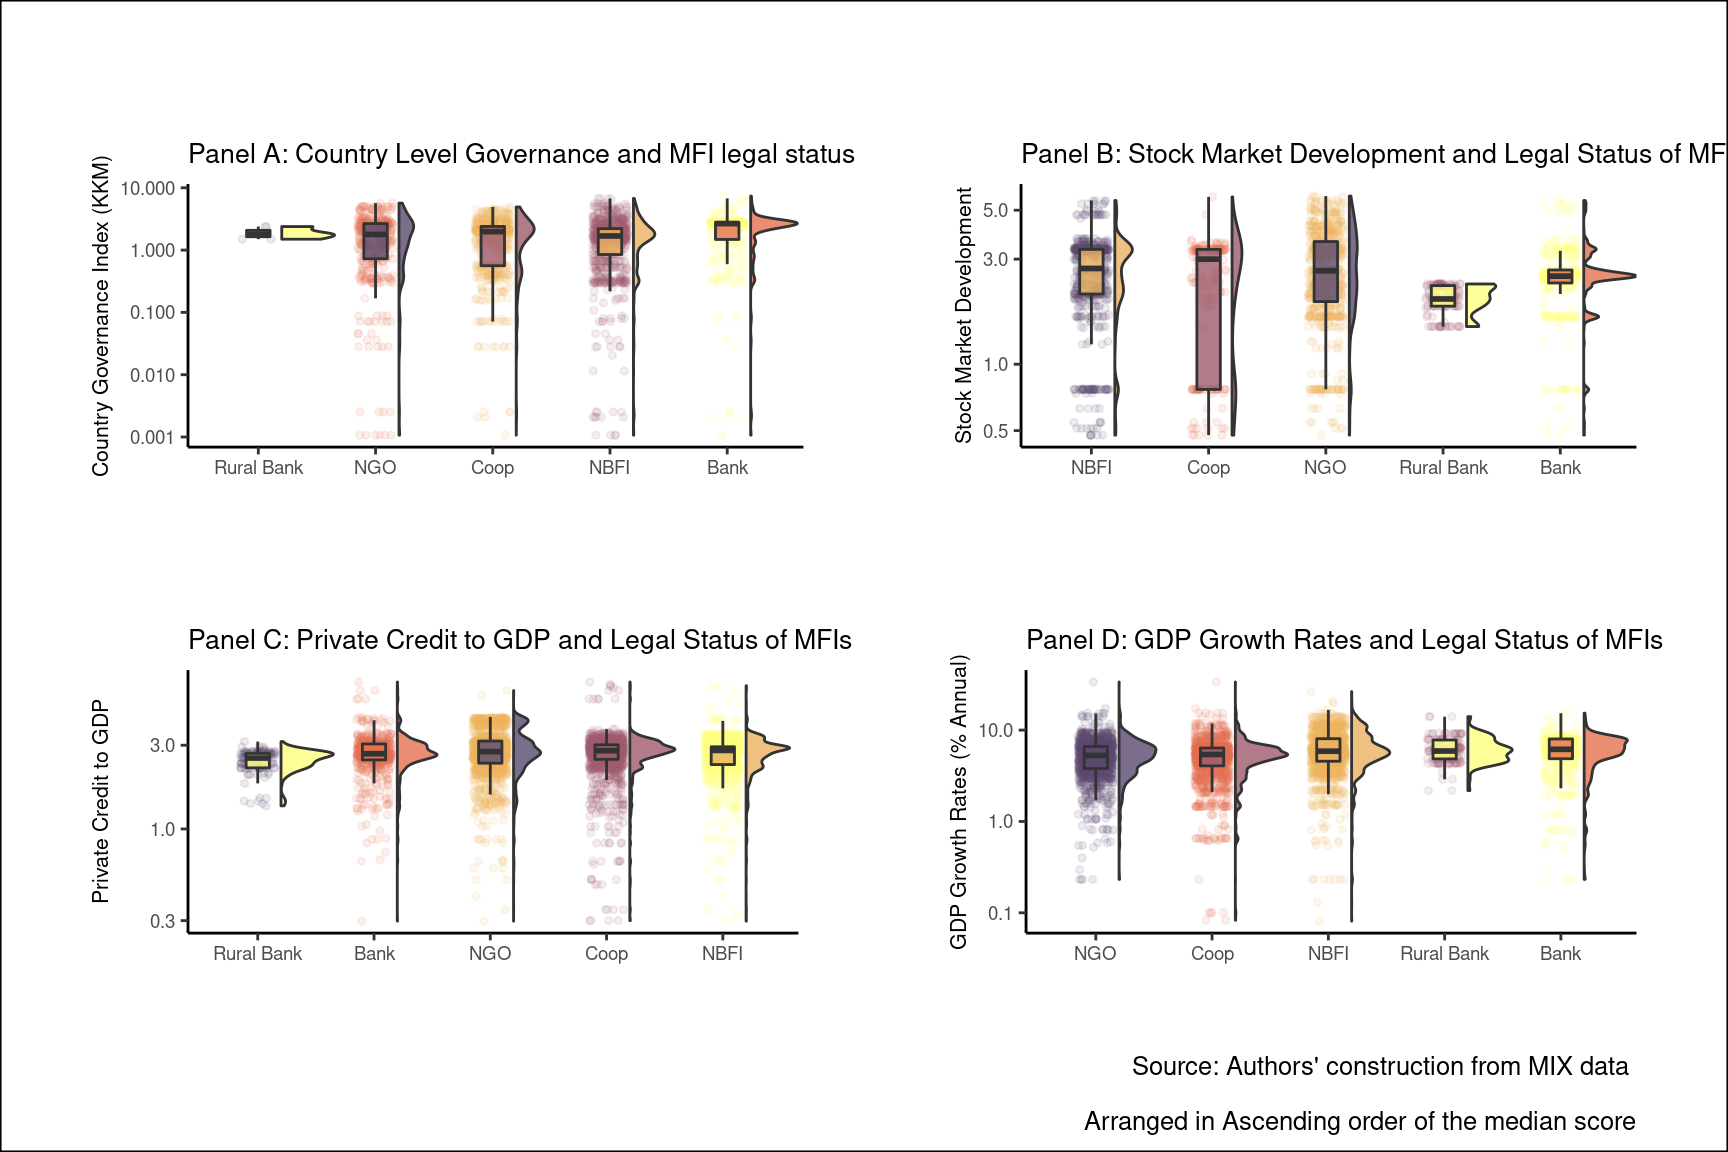
\includegraphics{_main_files/figure-latex/unnamed-chunk-20-1.pdf}
\caption{\label{fig:unnamed-chunk-20}Governance, Capital Market Development and Legal Status of MFIs in Africa}
\end{figure}

\end{landscape}

\newpage

\hypertarget{summary-statistics}{%
\subsubsection{Summary Statistics}\label{summary-statistics}}

Categorical variables summarised in Table 2.2 have no missing values. There are 1,280 NGOs against 3502 MFIs that are either commercial banks (619), NBFIs (1318), cooperatives (1427), or rural banks (138). As noted, even with the transformation of MFIs, NGOs still form a substantial number of MFIs, with the country to country variations \autocite{d2017ngos}. While 2558 MFIs are mature, 1200 are new, and 1024 are young. The result may indicate a slowdown in the establishment of new MFIs as donations become more unreliable. 1877 MFIs are from common law countries, with Civil law countries accounting for 1849, while 1056 come from other legal traditions. It is notable, as shown in Appendix 6, that most countries in Africa are either common law (18) or civil law(19), with relatively fewer nations in the `other' legal traditions category (11) \autocite{oto2014distribution}. It is also worth noting that North Africa accounts for only 166 observations in the data against 4616 observations in the sample dataset. Table 2.3 shows the summary statistics for the numeric variables where assets, governance (KKM), and GDP growth rates account for the highest variation.

Table 2.4 and Table 2.5 shows that NGOs, NBFIs, and commercial banks dominate common law countries. In civil law countries, it is cooperatives, NGOs, and NFIs that are most prevalent. In other legal traditions, it is NBFIs and credit unions that dominate. The result could indicate that the relatively well-developed capital markets in common law countries allow private, for-profit MFIs to thrive while not displacing NGOs. It means that NGOs in common law countries mainly serve niche markets where commercial MFIs find it uneconomical to reach. The relatively weak capital markets in civil law countries mean that cooperatives are central, with NGOs playing a significant role. Commercial MFIs like commercial banks and cooperatives' presence is low due to capital constraints. Turning to age in Table 6, most of the mature MFIs in the sample data are cooperatives, NGOs, and commercial banks in that order, while most of the new MFIs are NBFIs, cooperatives and commercial banks respectively. The results could indicate the increasing acceptance of the commercial model with newer MFIs going commercial. Table 2.7 shows the correlation between age and size, with larger MFIs more likely to be older.

\begin{table}

\caption{\label{tab:unnamed-chunk-21}Summary statistics for categorical variables}
\centering
\fontsize{9}{11}\selectfont
\begin{tabu} to \linewidth {>{\raggedright}X>{\raggedright}X}
\toprule
Variable & Counts\\
\midrule
Current legal status dummy & Others: 3502, NGO: 1280\\
Current legal status & Cooperative: 1427, NBFI: 1318, NGO: 1280, Bank: 619\\
Age & Mature: 2558, New: 1200, Young: 1024\\
Legal\_tradition & Common: 1877, Civil: 1849, Others: 1056\\
Region & Sub-Saharan Africa: 4616, North Africa: 166\\
\bottomrule
\multicolumn{2}{l}{\rule{0pt}{1em}Source: Authors' construction from MIX data}\\
\end{tabu}
\end{table}

\begin{table}

\caption{\label{tab:unnamed-chunk-22}Summary statistics for numeric variables}
\centering
\fontsize{9}{11}\selectfont
\begin{tabu} to \linewidth {>{\raggedright}X>{\raggedleft}X>{\raggedleft}X>{\raggedleft}X>{\raggedleft}X>{\raggedleft}X>{\raggedleft}X>{\raggedleft}X>{\raggedleft}X}
\toprule
Variable & N & Mean & SD & Min & Q1 & Median & Q3 & Max\\
\midrule
assets & 4782 & 14.946 & 2.262 & 0.693 & 13.540 & 14.858 & 16.416 & 22.98\\
kkm & 4782 & 0.003 & 2.006 & -5.233 & -1.304 & -0.114 & 1.628 & 7.37\\
education & 4782 & 0.387 & 0.144 & 0.075 & 0.273 & 0.386 & 0.487 & 1.05\\
pcrdbgdp & 4782 & 2.719 & 0.685 & 0.298 & 2.386 & 2.758 & 3.052 & 6.88\\
stmktcap & 4782 & 1.141 & 1.473 & 0.000 & 0.000 & 0.000 & 2.428 & 5.80\\
\addlinespace
prbonds & 4782 & 0.632 & 1.093 & 0.000 & 0.000 & 0.000 & 1.130 & 4.36\\
gdp\_growth\_annual & 4782 & 5.310 & 3.590 & -46.082 & 4.000 & 5.420 & 6.723 & 33.63\\
\bottomrule
\multicolumn{9}{l}{\rule{0pt}{1em}Source: Authors' construction from MIX data}\\
\end{tabu}
\end{table}

\begin{table}

\caption{\label{tab:unnamed-chunk-23}Legal Status of MFIs in Africa Disaggregated by Legal Tradition}
\centering
\fontsize{9}{11}\selectfont
\begin{tabu} to \linewidth {>{\raggedright}X>{\raggedleft}X>{\raggedleft}X>{\raggedleft}X>{\raggedleft}X>{\raggedleft}X}
\toprule
  & NGO & Bank & NBFI & Coop & Rural Bank\\
\midrule
Common & 0.323 & 0.246 & 0.310 & 0.048 & 0.073\\
Civil & 0.304 & 0.014 & 0.158 & 0.524 & 0.001\\
Other & 0.106 & 0.126 & 0.420 & 0.348 & 0.000\\
\bottomrule
\multicolumn{6}{l}{\rule{0pt}{1em}Source: Authors' construction from MIX data}\\
\multicolumn{6}{l}{\rule{0pt}{1em}\textit{Note: }}\\
\multicolumn{6}{l}{\rule{0pt}{1em}\textsuperscript{1} Horizontals total to 100}\\
\end{tabu}
\end{table}

\newpage

\hypertarget{results-of-the-regression-model}{%
\subsection{Results of the Regression Model}\label{results-of-the-regression-model}}

Table 2.11 shows the output from both the logit and probit regression analysis. We ran the analysis using the entire dataset, then filter MFIs with three or more years and five or more years of data and rerun the regression (as indicated in the bottom panel of the regression tables). We also include a time dummy, although these results are not in the regression tables. However, there is also a robust positive time trend towards commercialisation of MFIs, indicating relatively fewer NGO type MFIs over time as more MFIs opt for the commercial model. The trend is indicative of the gains that the sustainability school has made. However, NGOs still form a substantial proportion of MFIs. In this section, we examine each variable and its relative contribution to the transformation of MFIs. Note that we use the logit model in column 1 of Table 2.9 to interpret the discussion results. However, the interpretation is also applicable to the other models presented in Table 2.9.

\begin{table}

\caption{\label{tab:unnamed-chunk-24}Breakdown of Legal Status of MFIs by Legal Traditions, Percent}
\centering
\fontsize{9}{11}\selectfont
\begin{tabu} to \linewidth {>{\raggedright}X>{\raggedleft}X>{\raggedleft}X>{\raggedleft}X>{\raggedleft}X>{\raggedleft}X}
\toprule
legal\_tradition & NGO & Bank & NBFI & Coop & Rural Bank\\
\midrule
Common & 47.34 & 74.47 & 44.2 & 6.38 & 99.275\\
Civil & 43.91 & 4.04 & 22.2 & 67.91 & 0.725\\
Other & 8.75 & 21.49 & 33.7 & 25.72 & -\\
\bottomrule
\multicolumn{6}{l}{\rule{0pt}{1em}Source: Authors' construction from MIX data}\\
\multicolumn{6}{l}{\rule{0pt}{1em}\textit{Note: }}\\
\multicolumn{6}{l}{\rule{0pt}{1em}\textsuperscript{1} Verticals total to 100}\\
\end{tabu}
\end{table}

\hypertarget{age}{%
\subsubsection{Age}\label{age}}

New MFIs are more likely to adopt a commercial model than either young or mature ones, given the coefficients' negative sign. The observation may reflect the increasing acceptance of the financial systems approach to microfinance, making it harder for new entrants to attract donor funding \autocite{d2017ngos}. We postulate that older MFIs, being the pioneers and hence already well-acquainted with donors, find it easier to raise funds through donations and elicit state subsidies \autocite{d2013unsubsidized,mia2017mission}. Established MFIs have a historical relationship with donors. They are likely to attract funds, more so from donors that favour the welfare approach to microfinance, to reach out to the financially excluded first before pursuing profits. The results are in line with those in Table 6, which shows the distribution of MFI legal status disaggregated by age. While only 18\% of NGOs are new, 27.3\% are young, while about 30\% are mature, an upward trend. By comparison, the other legal status either decline or are relatively constant.

\begin{table}

\caption{\label{tab:unnamed-chunk-25}Legal Status of MFIs in Africa Disaggregated by Age}
\centering
\fontsize{9}{11}\selectfont
\begin{tabu} to \linewidth {>{\raggedright}X>{\raggedleft}X>{\raggedleft}X>{\raggedleft}X>{\raggedleft}X>{\raggedleft}X}
\toprule
  & NGO & Bank & NBFI & Coop & Rural Bank\\
\midrule
New & 0.188 & 0.193 & 0.297 & 0.295 & 0.027\\
Young & 0.273 & 0.099 & 0.334 & 0.275 & 0.019\\
Mature & 0.303 & 0.112 & 0.242 & 0.309 & 0.034\\
\bottomrule
\multicolumn{6}{l}{\rule{0pt}{1em}Source: Authors' construction from MIX data}\\
\end{tabu}
\end{table}

The coefficients of the logit model show that young MFIs (4-8 years) are 0.474 as likely to be in the commercial category than the new MFIs (0-4 years), ceteris paribus. This result means that new MFIs are likely to be commercial while older MFIs are most likely NGOs. \footnote{Relative risk ratios allow for easier interpretation of the logit models. To compute the ratio, we exponentiate the coefficients. For instance, the coefficient for young MFIs is -0.747, so the relative risk ratio is \(e^{-0.747}\), which gives 0.474. In other words, the odds of having the commercial model of microfinance is 1 - 0.474 = 0.526 in the sample dataset.}, we find that keeping all the other variables constant, young MFIs roughly one half less likely to be commercial than new MFIs. Likewise, mature MFIs are a third as likely to be commercial compared to new MFIs \footnote{Again, we exponentiate the coefficient -1.2 to get \(e^{-1.2} = 0.301\)}. The finding is also consistent with the intense time effect towards commercialisation which points to the increased acceptance of the commercial model of MFIs. The probit model also shows similar results.

Having started their operations before the neo-liberal tradition took hold, older MFIs have created goodwill with donors that enable them to solicit donations and subsidies easily. Mature MFIs could also have evolved business models to be financially sustainable without converting to the commercial model. For instance, mature MFIs tend to have a broader asset base meaning they have a more diverse customer base (see Table 6). Besides, they may have emphasised the social mission in their vision, mission, and organisational cultures to such an extent that both the MFI and the donor community find it hard to pull back \autocite{ramus2017,berbegal2019impact}.

\begin{table}

\caption{\label{tab:unnamed-chunk-26}Size (Assets) of MFIs in Africa Disaggregated by Age}
\centering
\fontsize{9}{11}\selectfont
\begin{tabu} to \linewidth {>{\raggedright}X>{\raggedleft}X>{\raggedleft}X>{\raggedleft}X>{\raggedleft}X}
\toprule
Age & Min\_size & Mean\_size & Median\_size & Max\_size\\
\midrule
New & 0.693 & 13.5 & 13.5 & 23.0\\
Young & 5.796 & 14.5 & 14.4 & 19.8\\
Mature & 6.361 & 15.8 & 15.7 & 22.9\\
\bottomrule
\multicolumn{5}{l}{\rule{0pt}{1em}Source: Authors' construction from MIX data}\\
\end{tabu}
\end{table}

Younger MFIs, on the other hand, cropped up when the paradigm shift to the institutional approach was taking shape. It means, therefore, that donors were reluctant to extend funds to such organisations. Hence, the MFIs had to supplement the little donor funding and government subsidies by raising funds from the capital markets. The thinking is consistent with the literature that shows the extent to which donor funding is volatile and especially sensitive to geopolitical realignments \autocite{garmaise2013cheap,d2017aid} and business cycles \autocite{wagner2013vulnerability}.

\hypertarget{legal-tradition}{%
\subsubsection{Legal Tradition}\label{legal-tradition}}

As noted, we have grouped countries in the sample data into their respective legal traditions following \textcite{oto2014distribution}. MFIs in civil law countries have a lower chance of transformation compared to those from common law countries \footnote{Appendix 6 shows a breakdown of the legal traditions in Africa}. However, MFIs in countries under ``other'' legal traditions have the highest likelihood of adopting the commercial model. The result is in line with the literature that shows the law's central place in finance \autocite{la2013law}. Specifically, holding all other variables constant, MFIs in civil law countries are 0.656 (\(e^{-0.421}\)) as likely as those in common law countries to follow the commercial model, meaning that most of them remain NGOs, following the not-for-profit, welfare approach. The odds of MFIs in civil law countries being commercial is 0.344 (\(1 - 0.656\)). On the contrary, MFIs in countries that follow other legal traditions are twice (\(e^{0.744}\)) as likely to be commercial instead of NGOs, with the odds being 1.1 (\(2.1 - 1.1\)).

Table 2.4 show the breakdown of MFI legal forms by the country's legal tradition. The Table shows the dominance of NGOs (32.3\%), commercial banks (24.6\%) and NBFIs (31\%) in common law countries. Cooperatives (52.4\%), NGOs (30.4\%), and NBFIs (15.8\%) dominate civil law countries, while NBFIs (42\%), cooperatives (34.8\%), and banks (12.6\%) are more common in other legal traditions. There are very few banks (1.4\%) and NBFIs (15.8\%) in civil law countries. Given the low levels of financial development in many civil law countries, there is a commercially viable gap for profit-oriented MFIs to fill. The gap raises the odds of MFI transformation happening more frequently in civil law countries than in countries following common law and other legal traditions.

On the contrary, the prevalence of commercial MFIs in common law countries could hold due to the higher levels of capital market development, reflecting the relative ease of acquiring funds \autocite{schnyder2018twenty}. The relative ease of acquiring capital from stock and bond markets could make it less likely that NGOs would prevail, making the commercial model more likely. The substantial number of NGOs in common law countries would fill the gap left by commercial MFIs due to the infeasibility of serving some clients, for instance, due to geographic remoteness or extreme poverty. There is little literature in law and finance that examines other legal traditions, such as Portuguese/ Spanish traditions as in Mozambique, Angola, Equatorial Guinea, and countries with unique traditions like Ethiopia that was never a colony. The results for the ``other'' legal practices in Africa's setting warrant further analysis. Table 2.5 confirms these results, showing, for instance, that 47.34\% of NGOs are in common law countries, 43.91 in civil law countries and the rest in other legal traditions. Common law countries have the bulk of banks (74.47\%) and NBFIs (44.2\%). Rural banks are almost entirely a common law phenomenon.

\hypertarget{size-log-of-total-assets}{%
\subsubsection{Size (Log of Total Assets)}\label{size-log-of-total-assets}}

All else being constant, larger MFIs in terms of assets are more likely to adopt the commercial model than the relatively smaller MFIs with fewer assets. Perhaps large MFIs can sustain their operations independent of donations and subsidies \autocite{d2013unsubsidized}. They have a higher capacity to attract money from the capital markets, given their strong assets base (as collateral) and track record. Everything else remaining the same, a unit increase in the asset base of an MFI raises the probability of transformation by 1.27 (\(e^{0.240}\)), with the odds of being in the commercial model being 0.27 (\(1.27 - 1\)).

Abundant literature in Africa and beyond, such as \textcite{gwatidzo2009corporate} and \textcite{kodongo2015capital}, show that the size of an MFI is an essential determinant of firms' capital structures, the mix of long term sources of funds. In this case, larger firms could easily avail collateral for funds and tend to be more open in providing information that financial intermediaries require to assess creditworthiness. On the other hand, small firms are informationally opaque \autocite{beck2014sme,kersten2017small}. Small firms, for example, may not afford to generate audited financial reports. Moreover, larger firms are likely to be mature with a solid business record, creating goodwill among the providers of funds \autocite{beck2008finance}. The size of MFIs could also reflect the extent of property rights protection that is harder to enforce in countries with weak governance \autocite{johnson2002property,claessens2003financial}. A fragile institutional environment makes it difficult for firms to grow due, in part, to poor access to capital and the high costs of formalising business \autocite{hansen2004reconsidering}. Next, we examine country-level governance / institutional quality.

\hypertarget{country-level-governance-institutional-quality-kkm}{%
\subsubsection{Country Level Governance/ Institutional Quality (KKM)}\label{country-level-governance-institutional-quality-kkm}}

We capture governance or institutional quality by taking the first principal component of the KKM Worldwide Governance Indicators (WGI) indices \autocite{kraay2010worldwide}. Governance (KKM Index) positively relates to the odds of transforming. All else remaining the same, when the governance index in a country rises by one unit, MFIs in the given country are 1.1 (\(e^{0.095}\)) times more likely to be in the commercial model than NGOs, meaning that the odds rise by \(0.1\) (\(1.1 - 1\)). The results probably hold due to the importance of property rights in raising confidence among private investors who finance the operations of transformed MFIs (Allen et al., 2013, 2014). Where governance and property rights are weak, most MFIs would likely remain NGOs for longer as investors are reluctant to finance private ventures in line with \textcite{johnson2002property} and \textcite{claessens2003financial}.

Literature shows a positive link between country-level institutional quality and the establishment, growth of private firms \autocite{sobel2008testing}. As captured in the KKM index, institutional quality captures factors that relate directly to the ease of doing business, contract enforcement effectiveness, and the extent of property rights. Where institutional quality is high, we expect private firms to take root, mainly commercial MFIs, primarily commercial banks and NBFIs. On the other hand, where institutional quality is low, NGOs and not-for-profit oriented MFIs may be more prevalent \autocite{kuzey2021link}. Indeed, The results on governance could partly explain the prevalence of NGOs in North Africa in the sample dataset, together with religion. Table 2.8 shows that North Africa fares poorly compared to Sub-Saharan Africa in most governance metrics. Interestingly, Table 2.9 shows that commercial banks and NBFIs are more prevalent in countries with higher institutional quality.

\begin{table}

\caption{\label{tab:unnamed-chunk-27}Summary Statistics on Governance in Africa}
\centering
\fontsize{9}{11}\selectfont
\begin{tabu} to \linewidth {>{\raggedright}X>{\raggedleft}X>{\raggedleft}X>{\raggedleft}X>{\raggedleft}X}
\toprule
Region & Min & Mean & Median & Max\\
\midrule
North Africa & -3.01 & -1.61 & -1.506 & -1.01\\
Sub-Saharan Africa & -5.23 & 0.06 & -0.114 & 7.37\\
\bottomrule
\multicolumn{5}{l}{\rule{0pt}{1em}Source: Authors' construction from MIX data}\\
\end{tabu}
\end{table}

\begin{table}

\caption{\label{tab:unnamed-chunk-28}Institutional Quality (KKM) and Legal Status of MFIs in Africa}
\centering
\fontsize{9}{11}\selectfont
\begin{tabu} to \linewidth {>{\raggedright}X>{\raggedleft}X>{\raggedleft}X>{\raggedleft}X>{\raggedleft}X}
\toprule
currentlegalstatus & Min & Mean & Median & Max\\
\midrule
NGO & -5.23 & -0.494 & -0.758 & 5.68\\
Bank & -5.23 & 0.929 & 1.208 & 7.37\\
NBFI & -5.17 & 0.510 & 0.350 & 6.74\\
Coop & -3.36 & -0.166 & -0.270 & 4.92\\
Rural Bank & -3.31 & -2.652 & -3.183 & 2.38\\
\bottomrule
\multicolumn{5}{l}{\rule{0pt}{1em}Source: Authors' construction from MIX data}\\
\end{tabu}
\end{table}

\hypertarget{private-credit-to-gdp}{%
\subsubsection{Private Credit to GDP}\label{private-credit-to-gdp}}

The private credit to GDP inversely relates to the prevalence of commercial models of microfinance, with the relationship primarily insignificant. In this case, private credit refers to an aspect of capital markets development, mainly in the banking sector. It is puzzling that a well-developed credit market does not appear to enhance the prevalence of for-profit MFI models. The results could suggest a weak linkage between MFIs and private capital markets, more so credit from financial intermediaries. Indeed, MFIs exist to serve markets where mainstream intermediaries neglect, meaning the low presence of mainstream banks means a higher prevalence of MFIs to fill the void \autocite{de2007economics}. Where significant, a unit increase in private credit to GDP corresponds to a 0.894 times lower chance that an MFI will be commercial, profit-oriented (\(e^{-0.112}\)), which corresponds to an odds of -0.114.

As noted, MFIs, especially the NGO type, exist to fill a financing gap that results from the failure of credit markets to reach the financially excluded, that is, the poor, rural dwellers and women savers and borrowers. If mainstream credit markets are functional, then there is no case for the existence of commercial MFIs, because mainstream banks would fill the gap adequately, leaving no business case for commercial MFIs to exist. However, as no credit market is fully efficient, then NGOs would exist to serve niche markets where financial sustainability is unattainable due to a combination of high costs and low revenues \autocite{de2007economics}. On the other hand, if capital markets are not well developed, there exists a market gap that commercial MFIs could exploit to make a profit \autocite{d2013unsubsidized,armendariz2013subsidy}.

\hypertarget{stock-market-capitalisation-to-gdp}{%
\subsubsection{Stock market capitalisation to GDP}\label{stock-market-capitalisation-to-gdp}}

Stock market capitalisation to GDP has a significant negative relationship with the prevalence of commercial MFIs. Precisely, a unit increase of stock market capitalisation corresponds to a 0.721 odds of an MFI adopting the for-profit model. Like private credit to GDP, stock market capitalisation to GDP proxies the level of stock market development, an essential source of long-term finance for corporations, presumably including MFIs. The equity could be from the public or private equity market, which the stock market would proxy reasonably well. In the case of MFIs in the sample dataset, the capital to assets ratio, the ratio of equity capital to assets, shows the importance of equity in financing microfinance. Notably, equity is of greater importance to NGOs than commercial MFIs (see Table 2.10), with NBFIs and commercial banks following in that order. If NGOs are the dominant participants in equity markets, there are lower chances that a well-developed stock market corresponds to more commercial MFIs. The same argument follows that if stock markets are well developed, private and, public credit markets are also well-developed \autocite{schnyder2018twenty}. With well-developed capital markets, financial exclusion incidences are fewer, leaving no vacuum that commercial MFIs could profitably exploit. In such instances, NGOs following the not-for-profit welfare model best serve the few cases of financial exclusion.

\begin{table}

\caption{\label{tab:unnamed-chunk-29}Capital Asset Ratio by MFI Legal Status in Africa}
\centering
\fontsize{9}{11}\selectfont
\begin{tabu} to \linewidth {>{\raggedright}X>{\raggedleft}X>{\raggedleft}X}
\toprule
Legal Status & Mean & Median\\
\midrule
Bank & 0.306 & 0.239\\
Credit Union/ Cooperative & 0.196 & 0.208\\
NBFI & 0.388 & 0.324\\
NGO & 0.418 & 0.381\\
Rural Bank & 0.176 & 0.137\\
\bottomrule
\multicolumn{3}{l}{\rule{0pt}{1em}Source: Authors' construction from MIX data}\\
\end{tabu}
\end{table}

\hypertarget{gdp-annual-growth-rate}{%
\subsubsection{GDP Annual Growth Rate}\label{gdp-annual-growth-rate}}

The GDP growth rate is not a significant driver of transformation. Where significant, some of the coefficients are positive, while others are negative. The implication is that the macro-environment may not be a substantial driver of MFIs decisions. Most MFIs in developing countries serve the informal sector's financially excluded population with low linkage to the formal economy \autocite{ghosh2013microfinance}.

\hypertarget{time-effects}{%
\subsubsection{Time Effects}\label{time-effects}}

The regression model also incorporates year effects, although not reported in the regression results tables. There is a strong trend towards commercialisation, with the commercial model increasingly dominating Africa's MFI landscape. All the year dummies are significant in all the models, the lowest level of significance being 10\%. Numerous researchers have noted the trend towards the commercial model. Hence, the abundant research seeks to examine the potential effects of the transformation on financial inclusion targets- the financially excluded \autocite{d2017ngos}. Some scholars claim that the trend may harm financial inclusion. \autocite{meagher2006microfinance,hartarska2007regulated}. Others hold the opposing view \autocite{duvendack2015mis}. It appears that the financial sustainability school that seeks commercialisation has the upper hand in Africa, at least in the last two decades.

\hypertarget{regional-divide}{%
\subsubsection{Regional Divide}\label{regional-divide}}

It is notable that for the sample data, all the MFIs operating in North Africa are NGOs, while the rest of Africa has a MIX of all forms of MFIs \footnote{Countries in North Africa in the sample data are Morocco and Tunisia}. Religion may be at play in this case, where interest-based for-profit lending is incompatible with the Muslim faith that dominates North Africa \autocite{hassan2018religious}. Also, as noted, North Africa fares worse in governance (KKM) than sub-Saharan Africa, leading to a flawed property rights regime that discourages private investment \autocite{johnson2002property,claessens2003financial}.

\newpage

\begin{landscape}

\begin{table}[!htbp] \centering 
  \caption{Logit and Probit Models (Standard Errors in Brackets)} 
  \label{} 
\footnotesize 
\begin{tabular}{@{\extracolsep{5pt}}lcccccccc} 
\\[-1.8ex]\hline 
\hline \\[-1.8ex] 
 & \multicolumn{8}{c}{\textit{Dependent variable:}} \\ 
\cline{2-9} 
\\[-1.8ex] & \multicolumn{8}{c}{Dummy: Current Legal Status} \\ 
\\[-1.8ex] & \textit{logistic} & \textit{probit} & \textit{logistic} & \textit{probit} & \textit{logistic} & \textit{probit} & \textit{logistic} & \textit{probit} \\ 
\\[-1.8ex] & (1) & (2) & (3) & (4) & (5) & (6) & (7) & (8)\\ 
\hline \\[-1.8ex] 
 ageYoung & $-$0.747$^{***}$ & $-$0.421$^{***}$ & $-$0.418$^{***}$ & $-$0.240$^{***}$ & $-$0.452$^{***}$ & $-$0.264$^{***}$ & $-$0.766$^{***}$ & $-$0.431$^{***}$ \\ 
  & (0.114) & (0.065) & (0.132) & (0.076) & (0.157) & (0.091) & (0.112) & (0.064) \\ 
  & & & & & & & & \\ 
 ageMature & $-$1.200$^{***}$ & $-$0.691$^{***}$ & $-$0.898$^{***}$ & $-$0.522$^{***}$ & $-$0.944$^{***}$ & $-$0.551$^{***}$ & $-$1.150$^{***}$ & $-$0.662$^{***}$ \\ 
  & (0.106) & (0.060) & (0.122) & (0.071) & (0.145) & (0.084) & (0.104) & (0.059) \\ 
  & & & & & & & & \\ 
 legal\_traditionCivil & $-$0.421$^{***}$ & $-$0.239$^{***}$ & $-$0.515$^{***}$ & $-$0.313$^{***}$ & $-$0.545$^{***}$ & $-$0.338$^{***}$ & $-$0.518$^{***}$ & $-$0.289$^{***}$ \\ 
  & (0.117) & (0.068) & (0.127) & (0.074) & (0.140) & (0.082) & (0.114) & (0.066) \\ 
  & & & & & & & & \\ 
 legal\_traditionOther & 0.744$^{***}$ & 0.387$^{***}$ & 0.790$^{***}$ & 0.416$^{***}$ & 0.870$^{***}$ & 0.466$^{***}$ & 0.743$^{***}$ & 0.387$^{***}$ \\ 
  & (0.132) & (0.073) & (0.149) & (0.084) & (0.167) & (0.094) & (0.130) & (0.072) \\ 
  & & & & & & & & \\ 
 assets & 0.240$^{***}$ & 0.142$^{***}$ & 0.355$^{***}$ & 0.214$^{***}$ & 0.450$^{***}$ & 0.270$^{***}$ & 0.242$^{***}$ & 0.144$^{***}$ \\ 
  & (0.019) & (0.011) & (0.024) & (0.014) & (0.029) & (0.016) & (0.018) & (0.011) \\ 
  & & & & & & & & \\ 
 kkm & 0.095$^{***}$ & 0.057$^{***}$ & 0.102$^{***}$ & 0.063$^{***}$ & 0.139$^{***}$ & 0.087$^{***}$ & 0.115$^{***}$ & 0.067$^{***}$ \\ 
  & (0.019) & (0.011) & (0.023) & (0.013) & (0.025) & (0.015) & (0.019) & (0.011) \\ 
  & & & & & & & & \\ 
 pcrdbgdp & $-$0.112 & $-$0.049 & $-$0.127 & $-$0.047 & $-$0.221$^{**}$ & $-$0.097$^{*}$ & 0.055 & 0.036 \\ 
  & (0.076) & (0.042) & (0.083) & (0.047) & (0.090) & (0.051) & (0.070) & (0.039) \\ 
  & & & & & & & & \\ 
 stmktcap & $-$0.327$^{***}$ & $-$0.190$^{***}$ & $-$0.369$^{***}$ & $-$0.225$^{***}$ & $-$0.398$^{***}$ & $-$0.246$^{***}$ & $-$0.359$^{***}$ & $-$0.206$^{***}$ \\ 
  & (0.038) & (0.022) & (0.042) & (0.024) & (0.047) & (0.027) & (0.037) & (0.021) \\ 
  & & & & & & & & \\ 
 gdp\_growth\_annual & 0.016 & 0.012$^{*}$ & $-$0.004 & $-$0.0004 & $-$0.025$^{*}$ & $-$0.013 & 0.024$^{**}$ & 0.015$^{**}$ \\ 
  & (0.011) & (0.006) & (0.013) & (0.008) & (0.014) & (0.008) & (0.011) & (0.006) \\ 
  & & & & & & & & \\ 
\hline \\[-1.8ex] 
Year Effects & Yes & Yes & Yes & Yes & Yes & Yes & No & No \\ 
Deviance & 677*** & 664*** & 651*** & 648*** & 660*** & 659*** & 619*** & 607*** \\ 
Data & Full & Full & >3yrs & >3yrs & >5yrs & >5yrs & Full & Full \\ 
Observations & 4,782 & 4,782 & 3,840 & 3,840 & 3,165 & 3,165 & 4,782 & 4,782 \\ 
Log Likelihood & $-$2,439.000 & $-$2,446.000 & $-$2,004.000 & $-$2,005.000 & $-$1,633.000 & $-$1,633.000 & $-$2,469.000 & $-$2,475.000 \\ 
Akaike Inf. Crit. & 4,939.000 & 4,952.000 & 4,068.000 & 4,071.000 & 3,325.000 & 3,326.000 & 4,957.000 & 4,969.000 \\ 
\hline 
\hline \\[-1.8ex] 
\textit{Note:}  & \multicolumn{8}{l}{$^{*}$p$<$0.1; $^{**}$p$<$0.05; $^{***}$p$<$0.01} \\ 
\end{tabular} 
\end{table}

\end{landscape}

\newpage

\hypertarget{multinomial-logit-model}{%
\subsection{Multinomial Logit Model}\label{multinomial-logit-model}}

We extend the analysis to the multinomial logit model. To reiterate, the multinomial logit model will help uncover factors that drive the choice of a particular legal form by NGOs adopting the commercial model. We present the results of the model in the tables of Appendix 2 through to Appendix 5. As in the binary models, the results confirm the factors that drive the conversion of MFIs from NGOs to commercial models. We base our discussion on the results in Appendix 2, which easily generalises to the other appendices. The results show that as the MFI transitions from being new to young, it is less likely to be a bank, NBFI, credit union, or rural bank due to the coefficients' negative sign. Hence, older firms are more likely to be NGOs in line with the logit model for reasons expounded in the logit model's output.

Similarly, compared to NGOs, mature MFIs are less likely to be commercial banks, NBFIs, cooperatives or rural banks. The results align with the logit model showing that most commercial MFIs are more likely new or young, while NGOs are more likely mature. Again, start-up MFIs are more inclined to the commercial model than the established MFIs.

Relative to common law countries, MFIs in civil law countries are less likely to be commercial banks, NBFIs, and rural banks and are more likely to be NGOs. However, in civil law countries, MFIs are more likely to be cooperatives than NGOs. Likewise, relative to common law countries, MFIs in other legal traditions are less likely to be commercial banks and rural banks than NGOs and more likely to be credit unions or NBFIs than NGOs. The results illustrate the link between legal tradition and the legal status of MFIs, with NGOs dominating common law countries whilst cooperatives prevail in other legal traditions, including civil law tradition. As noted, the better-developed capital markets in common law countries leave little room for commercial MFIs to thrive. On the contrary, the under-served populace in civil law countries presents ample business opportunities for profit-oriented MFIs \autocite{d2013unsubsidized,mia2017mission}.

The results show that as an MFI size increases, the likelihood of shifting from the NGO model to the commercial model rises. However, as firms grow in size, they are less likely to adopt the cooperative model, although the relationship is not significant. MFIs mainly shift from NGOs to commercial banks, rural banks, and NBFIs, but rarely to cooperatives or rural banks. The results highlight the uniqueness of cooperatives and rural banking as microfinance models that serve niche markets. Strictly speaking, cooperatives are quasi-commercial entities. Their mode of operation differs from the other MFIs in terms of clientele and possible geographic reach, reducing size. Similarly, rural banks serve marginalised rural dwellers and are more prevalent in common law countries. Noting that most large MFIs are also mature, it follows that the edge granted by maturity also accrues to larger MFIs \autocite{beck2014sme,kersten2017small}.

Also, as country-level institutional quality rises, MFIs are more likely to be commercial banks and NBFIs, and less likely cooperatives and rural banks relative to NGOs. Cooperatives and rural banks are less sensitive to institutional quality matters courtesy of their unique markets, even more so than NGOs \autocite{sobel2008testing}. As noted earlier, the commercial, for-profit model could only thrive best in countries where institutional quality is high. However, cooperatives and rural banks in Africa serve unique markets. Rural banks primarily focused on informal rural economies that may have a weak linkage to the formal economy, making governance and institutional quality less relevant.

By way of both stock market to GDP and private credit to GDP, capital market development follows a similar pattern. As in the logit model, MFIs in countries scoring high in private credit to GDP and stock market capitalisation to GDP are less likely to go commercial and more likely to be NGOs. We have argued before that well developed financial market implies a smaller customer base for MFIs and hence the result. The result also concurs with the observation about legal tradition. Because capital markets in civil law countries are less developed, the void tends to be profitably filled by commercial MFIs.In common law countries, capital markets leave few profitable opportunities which NGOs serve \autocite{d2013unsubsidized,armendariz2013subsidy}.

Finally, high GDP growth rates increase the likelihood that an MFI will be a commercial bank, NBFI, or rural bank than NGOs but less likely to be a cooperative or rural bank. As is the case with institutional quality, the economic environment matters most for commercial MFIs that target profit. However, NGOs, cooperatives and rural banks may better serve communities undergoing adverse economic experiences \autocite{ghosh2013microfinance}. Cooperatives obtain capital from members and are obligated to attend to the members regardless of economic uncertainties. NGOs and rural banks specifically target marginalised people. Economic downturns are more likely to raise the level of exclusion and make these forms of MFIs even more relevant \autocite{schnyder2018twenty}.

\hypertarget{overall-model-fit}{%
\subsection{Overall Model Fit}\label{overall-model-fit}}

To assess the overall model fit, we generate the \texttt{confusion\ matrix} and statistics in Table 2.12 and figure 4, respectively. For this purpose, we use the models developed by using the whole dataset- Table 2.11 for the logit model and Appendix 2 for the multinomial logit model.

\hypertarget{logit-model}{%
\subsubsection{Logit Model}\label{logit-model}}

Overall, the models are highly significant (at 1\% significance levels, see Table 2.11), meaning that they explain why MFIs tend to adopt a given model better than guessing the most prevalent outcome- that every MFI in the sample is not an NGO. In the first row of Table 2.12, we see that the logit model predicted correctly that 304 NGOs were NGOs. The model also accurately predicts that an MFI belongs to other legal forms (Bank, NBFI, Coop, Rural Bank) when they belong to these forms. However, the model fails by predicting 976 cases of MFIs as other legal forms when they are NGOs. Similarly, the model wrongly classifies 126 cases of MFIs of other legal forms as NGOs.

Overall, the logit model accurately predicts the legal status of an MFI 77\% of the time \footnote{The accuracy is computed as (304 + 3376)/(304 + 976 + 126 + 3376) = 0.77}. The prediction is within the confidence interval captured by the entries \texttt{AccuracyLower} and \texttt{AccuracyUpper}. If we were to guess that every MFI in the dataset follows the commercial model (that is, not an NGO), we would be accurate 73.2\% of the time (referred to as the No Information Rate (NIR) in the \texttt{confusion\ matrix}) \autocite{cavalin2018confusion}. The p-value shows that the accuracy is not due to chance with over 99\% confidence, meaning that the accuracy is significantly greater than the NIR \autocite{kleinbaum2002logistic}.

The model has low \texttt{sensitivity}, though, at 23.75\%. In this case, sensitivity is a model's ability to accurately predict that an MFI is an NGO when it is an NGO \autocite{marom2010using}. The low \texttt{sensitivity} could, in part, be due to the low \texttt{prevalence} of NGOs in the dataset (at 26.77\%) relative to the commercial forms of MFIs (73.23\%). However, the model has very high \texttt{specificity} at 96.4\%. Specificity is the capacity of the model to predict that an MFI follows the commercial model (NOT an NGO) when it is following the commercial model (is NOT an NGO) \autocite{zeng2020confusion}. Hence, it appears that commercial MFIs have distinct characters that easily allow the model to distinguish them from NGOs. The other metric of interest is the \texttt{balanced\ accuracy} that averages \texttt{sensitivity} and \texttt{specificity} at 60\% \autocite{gorzalczany2016multi}. Overall, the model does better than guessing that every MFI in the sample dataset follows the commercial model (or is NOT an NGO) \autocite{hosmer2013applied}.

Figure 2.4 shows a visualization of the confusion matrix and the receiver operating characteristics (ROC) curve. Again these visualizations show that the model does well in \texttt{specificity}. The ROC curve plots \texttt{sensitivity} against \(1 - specificity\). For an ideal model, the ROC curve would pass through the point (0,1), which is the top left corner of the curve. A model with a ROC curve being a straight line passing through the origin (the dotted line) does no better than guessing. In this case, the ROC curve shows that the model has significant explanatory power. A related metric the area under the ROC curve called the \texttt{area\ under\ the\ curve\ (AUC)} shown in Table 2.13. AUC is the area between the ROC curve and the x-axis, with higher values of AUC corresponding to a better model. An AUC of 0.5 connotes a model that discriminates the units of analysis no better than guessing and is equivalent to the straight line passing through the origin \autocite{mandrekar2010receiver}. The AUC, in this case, is 0.726 out of a possible maximum of one.

\begin{table}

\caption{\label{tab:unnamed-chunk-34}Confusion Matrix and Statistics for the Logit Model}
\centering
\fontsize{9}{11}\selectfont
\begin{tabu} to \linewidth {>{\raggedright}X>{\raggedright}X>{\raggedleft}X}
\toprule
.metric & .estimator & .estimate\\
\midrule
accuracy & binary & 0.770\\
kap & binary & 0.255\\
sens & binary & 0.238\\
spec & binary & 0.964\\
ppv & binary & 0.707\\
\addlinespace
npv & binary & 0.776\\
mcc & binary & 0.312\\
j\_index & binary & 0.202\\
bal\_accuracy & binary & 0.601\\
detection\_prevalence & binary & 0.090\\
\addlinespace
precision & binary & 0.707\\
recall & binary & 0.238\\
f\_meas & binary & 0.356\\
\bottomrule
\multicolumn{3}{l}{\rule{0pt}{1em}Source: Authors' construction}\\
\multicolumn{3}{l}{\rule{0pt}{1em}\textit{Notes: }}\\
\multicolumn{3}{l}{\rule{0pt}{1em}\textsuperscript{1} Accuracy > NoInformationRate is significant at 1\% confidence level, p = 0.0000}\\
\end{tabu}
\end{table}

\newpage
\begin{landscape}

\begin{table}

\caption{\label{tab:unnamed-chunk-35}ROC Area Under Curve (ROC AUC)}
\centering
\fontsize{9}{11}\selectfont
\begin{tabu} to \linewidth {>{\raggedright}X>{\raggedright}X>{\raggedleft}X}
\toprule
.metric & .estimator & .estimate\\
\midrule
roc\_auc & binary & 0.726\\
\bottomrule
\multicolumn{3}{l}{\rule{0pt}{1em}Source: Authors' construction}\\
\end{tabu}
\end{table}

\begin{figure}
\centering
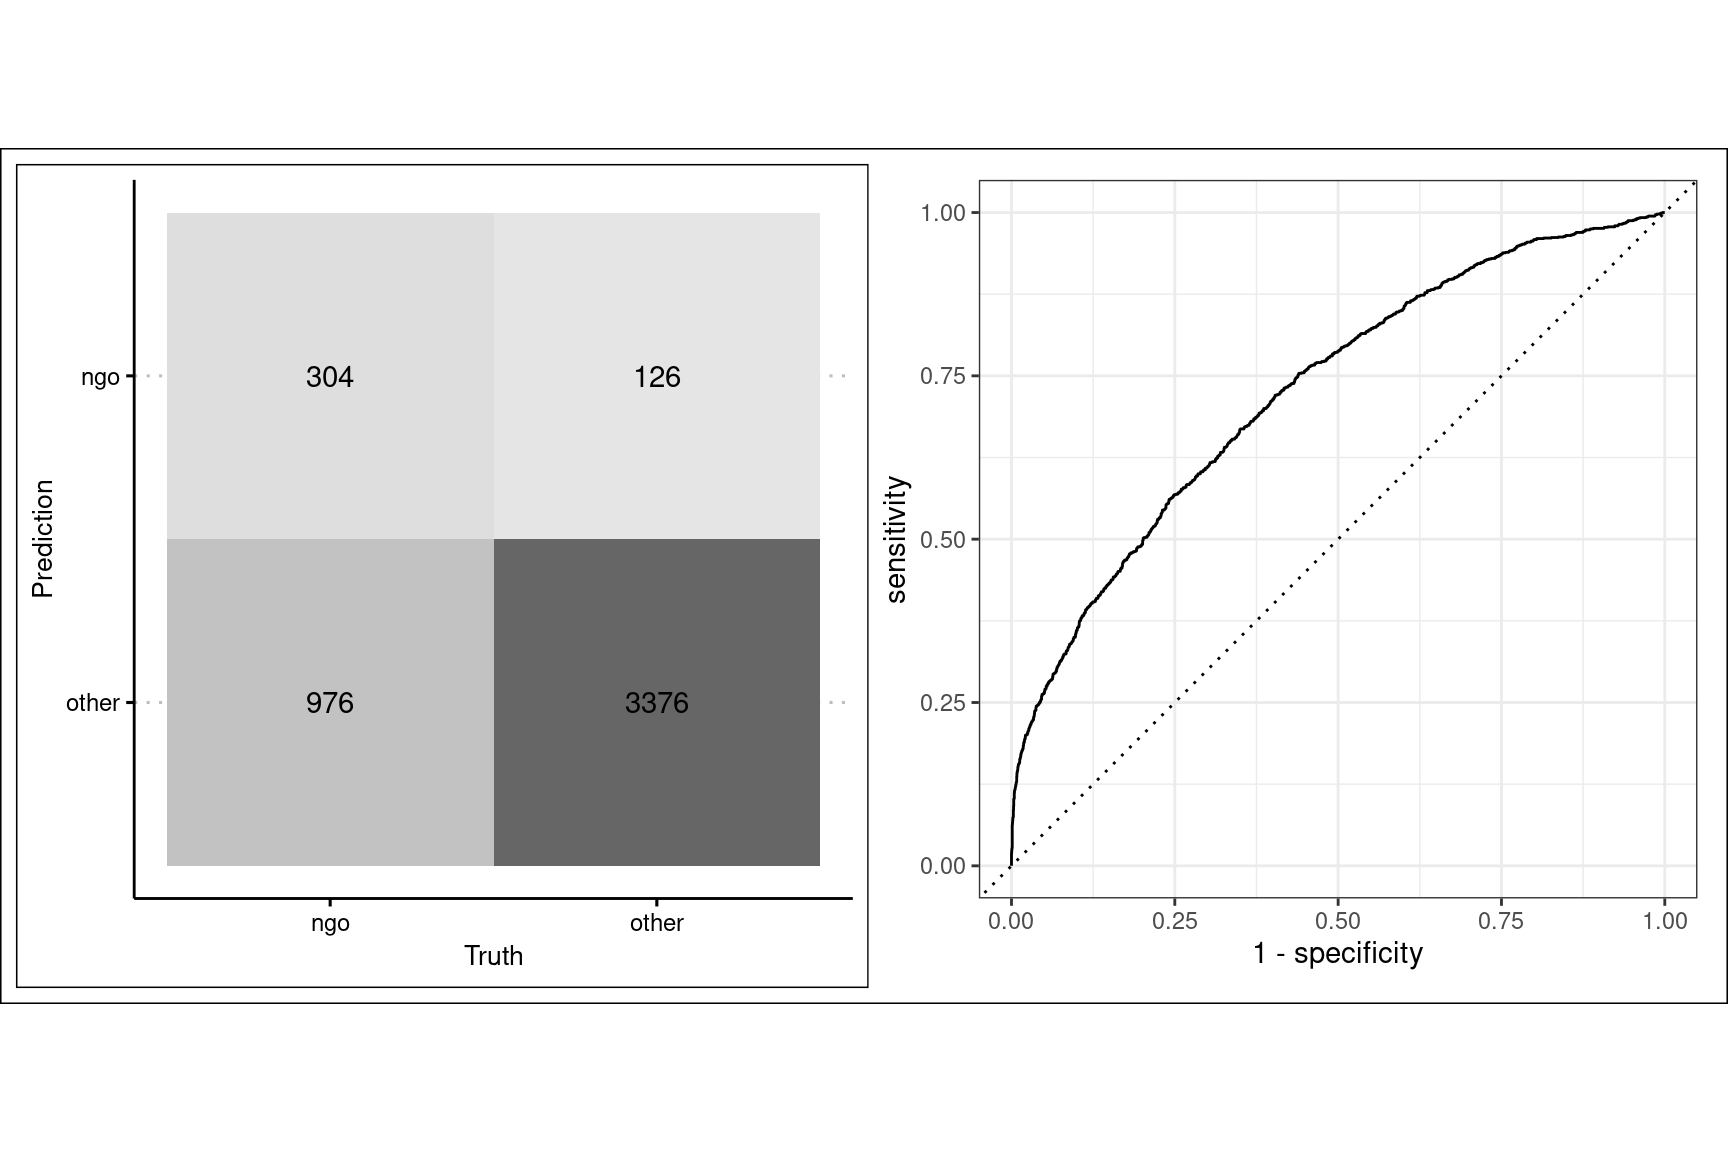
\includegraphics{_main_files/figure-latex/unnamed-chunk-35-1.pdf}
\caption{\label{fig:unnamed-chunk-35}Confusion Matrix (left) and ROC Curve}
\end{figure}

\newpage
\end{landscape}

\newpage

\hypertarget{multinomial-logit-model-1}{%
\subsubsection{Multinomial Logit Model}\label{multinomial-logit-model-1}}

The variables that are significant drivers of the transformation of MFIs under the logit and probit models are also significant in the multinomial logit model. We also generate the \texttt{confusion\ matrix} using the \texttt{multinomial\ logit} with the complete data (Table 2.14). The matrix shows that the overall \texttt{accuracy} is 56.5\%. Note that the overall accuracy is one value for the entire model, the \texttt{No\ Information\ Rate\ (NIR)}. Overall \texttt{accuracy}, in this case, is the ability to accurately predict that an MFI is an NGO when it is an NGO, a commercial bank when it is a commercial bank, and so on. If we were to guess that every MFI in the model is the cooperative - the most prevalent legal form- we would be right 39.3\% of the time, the NIR. The p-value shows that the overall \texttt{accuracy} metric is significantly different from the \texttt{NIR}. Although the multinomial logit model has a markedly lower accuracy than the logit model, it has a far more demanding task of distinguishing five legal forms of MFIs instead of 2 for the logit model \autocite{kwak2002multinomial}.

The model's \texttt{sensitivity} varies from a low of 47.1\% for NBFI to a high of 61.8\% for NGOs. The \texttt{specificity} is relatively high, ranging from 80.1\% for NBFIs to 99.22\% for rural banks \autocite{ginting2019hate}. NGOs have a \texttt{specificity} of 81.4\%, meaning that the model can predict that an MFI is not an NGO when it is not an NGO 81.4\% of the time. For rural banks, the model can correctly predict over 99\% of the time that an MFI is not a rural bank when it is not a rural bank. The \texttt{balanced\ accuracy} is also reasonably high, with the lowest being NBFIs at 63.9\% and the highest at 79.26\% for rural banks \autocite{hedeker2003mixed}.

\begin{table}

\caption{\label{tab:unnamed-chunk-36}Confusion Matrix and Statistics for the Multinomial Logit Model}
\centering
\fontsize{9}{11}\selectfont
\begin{tabular}[t]{llllll}
\toprule
  & NGO & Bank & NBFI & Coop & Rural Bank\\
\midrule
Accuracy & 0.565 & - & - & - & -\\
NoInformationRate & 0.393 & - & - & - & -\\
Kappa & 0.414 & - & - & - & -\\
sensitivity & 0.618 & 0.6154 & 0.478 & 0.584 & 0.5930\\
specificity & 0.814 & 0.9298 & 0.801 & 0.886 & 0.9922\\
\addlinespace
PosPredValue & 0.437 & 0.5170 & 0.474 & 0.768 & 0.7391\\
NegPredValue & 0.901 & 0.9520 & 0.803 & 0.767 & 0.9849\\
Prevalence & 0.189 & 0.1087 & 0.274 & 0.393 & 0.0360\\
DetectionRate & 0.117 & 0.0669 & 0.131 & 0.229 & 0.0213\\
DetectionPrevalence & 0.268 & 0.1294 & 0.276 & 0.298 & 0.0289\\
\addlinespace
BalancedAccuracy & 0.716 & 0.7726 & 0.639 & 0.735 & 0.7926\\
\bottomrule
\multicolumn{6}{l}{\rule{0pt}{1em}Source: Authors' construction}\\
\multicolumn{6}{l}{\rule{0pt}{1em}\textit{Notes: }}\\
\multicolumn{6}{l}{\rule{0pt}{1em}\textsuperscript{1} Accuracy, No information rate and Kappa are the same accross the legal forms of MFIs}\\
\multicolumn{6}{l}{\rule{0pt}{1em}\textsuperscript{2} Accuracy > NoInformationRate is significant at 1\% confidence level, p = 0.0000}\\
\end{tabular}
\end{table}

\newpage

\hypertarget{regression-diagnostics}{%
\subsection{Regression Diagnostics}\label{regression-diagnostics}}

This section examines three issues that arise in logit models: extreme values, multicollinearity, and linearity, respectively.

\hypertarget{extreme-values}{%
\subsubsection{Extreme values}\label{extreme-values}}

Figure 2.4 below shows that the data indeed has influential values. For robustness, we winsorise the data, removing the top 10\% and the bottom 10\%. Still, the results remain robust, as regression results in Table 2.14 show. It is notable that apart from the change in coefficients' value, the signs remain the same, meaning that influential observations (outliers) are not significant.

\begin{table}[!htbp] \centering 
  \caption{Regression Results - Logit and Probit Models for Winsorized Data} 
  \label{} 
\footnotesize 
\begin{tabular}{@{\extracolsep{5pt}}lcccc} 
\\[-1.8ex]\hline 
\hline \\[-1.8ex] 
 & \multicolumn{4}{c}{\textit{Dependent variable:}} \\ 
\cline{2-5} 
\\[-1.8ex] & \multicolumn{4}{c}{Dummy: Current Legal Status (Standard Errors in Brackets)} \\ 
\\[-1.8ex] & \textit{logistic} & \textit{probit} & \textit{logistic} & \textit{probit} \\ 
\\[-1.8ex] & (1) & (2) & (3) & (4)\\ 
\hline \\[-1.8ex] 
 ageYoung & $-$0.887$^{***}$ & $-$0.514$^{***}$ & $-$0.890$^{***}$ & $-$0.515$^{***}$ \\ 
  & (0.119) & (0.068) & (0.117) & (0.067) \\ 
  & & & & \\ 
 ageMature & $-$1.350$^{***}$ & $-$0.787$^{***}$ & $-$1.270$^{***}$ & $-$0.743$^{***}$ \\ 
  & (0.111) & (0.063) & (0.109) & (0.062) \\ 
  & & & & \\ 
 legal\_traditionCivil & $-$0.221$^{*}$ & $-$0.113 & $-$0.374$^{***}$ & $-$0.196$^{***}$ \\ 
  & (0.130) & (0.076) & (0.124) & (0.072) \\ 
  & & & & \\ 
 legal\_traditionOther & 0.913$^{***}$ & 0.500$^{***}$ & 0.893$^{***}$ & 0.486$^{***}$ \\ 
  & (0.146) & (0.081) & (0.142) & (0.079) \\ 
  & & & & \\ 
 assets & 0.272$^{***}$ & 0.161$^{***}$ & 0.273$^{***}$ & 0.164$^{***}$ \\ 
  & (0.021) & (0.012) & (0.020) & (0.012) \\ 
  & & & & \\ 
 kkm & 0.081$^{***}$ & 0.050$^{***}$ & 0.111$^{***}$ & 0.068$^{***}$ \\ 
  & (0.021) & (0.012) & (0.020) & (0.012) \\ 
  & & & & \\ 
 pcrdbgdp & $-$0.330$^{***}$ & $-$0.187$^{***}$ & $-$0.075 & $-$0.048 \\ 
  & (0.098) & (0.056) & (0.086) & (0.050) \\ 
  & & & & \\ 
 stmktcap & $-$0.269$^{***}$ & $-$0.152$^{***}$ & $-$0.326$^{***}$ & $-$0.183$^{***}$ \\ 
  & (0.044) & (0.025) & (0.041) & (0.024) \\ 
  & & & & \\ 
 gdp\_growth\_annual & 0.026 & 0.018$^{*}$ & 0.037$^{**}$ & 0.024$^{**}$ \\ 
  & (0.018) & (0.010) & (0.017) & (0.010) \\ 
  & & & & \\ 
 Constant & $-$2.140$^{***}$ & $-$1.310$^{***}$ & $-$1.690$^{***}$ & $-$1.050$^{***}$ \\ 
  & (0.485) & (0.288) & (0.325) & (0.191) \\ 
  & & & & \\ 
\hline \\[-1.8ex] 
Year Effects & Yes & Yes & No & No \\ 
Deviance & 664*** & 657*** & 602*** & 595*** \\ 
df & 29 & 29 & 9 & 9 \\ 
Data & Winsorized & Winsorized & Winsorized & Winsorized \\ 
Observations & 4,474 & 4,474 & 4,474 & 4,474 \\ 
Log Likelihood & $-$2,282.000 & $-$2,285.000 & $-$2,314.000 & $-$2,318.000 \\ 
Akaike Inf. Crit. & 4,623.000 & 4,631.000 & 4,648.000 & 4,655.000 \\ 
\hline 
\hline \\[-1.8ex] 
\textit{Note:}  & \multicolumn{4}{l}{$^{*}$p$<$0.1; $^{**}$p$<$0.05; $^{***}$p$<$0.01} \\ 
\end{tabular} 
\end{table}

\begin{landscape}

\begin{figure}
\centering
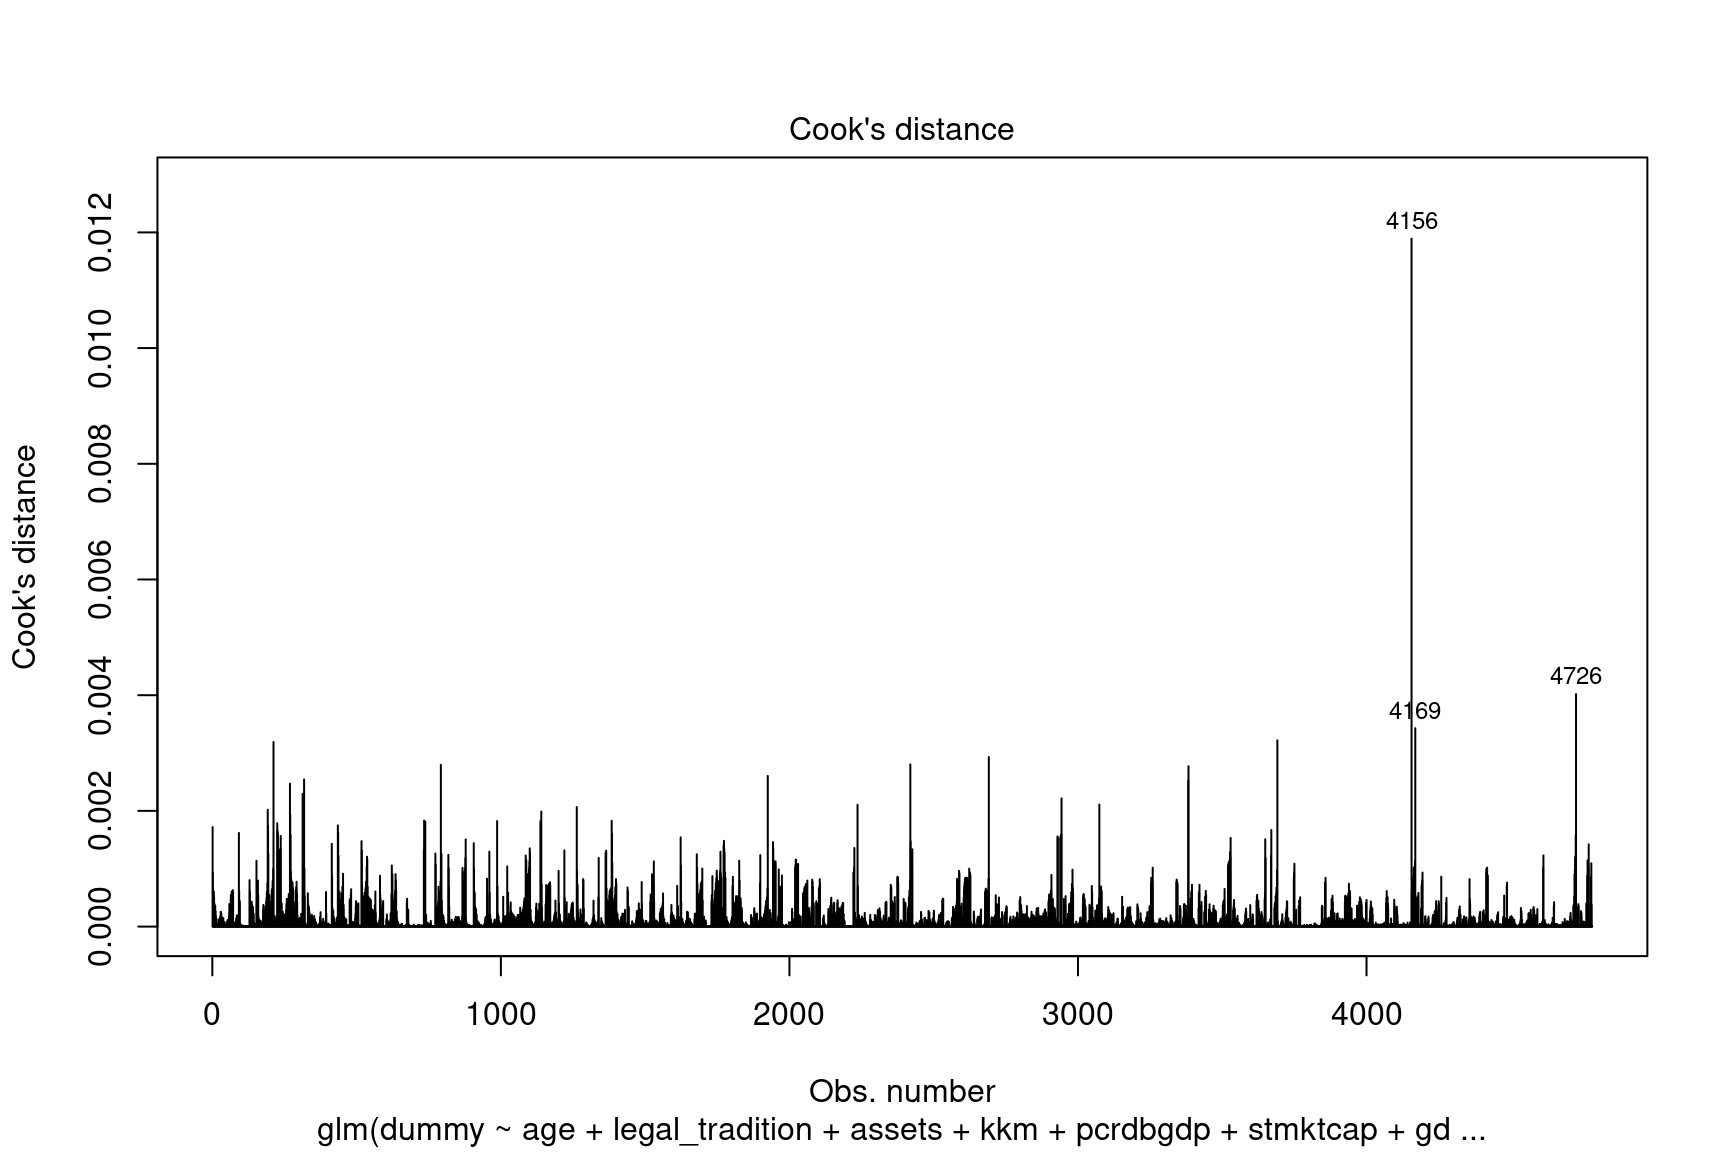
\includegraphics{_main_files/figure-latex/unnamed-chunk-40-1.pdf}
\caption{\label{fig:unnamed-chunk-40}Visualisation of Outliers}
\end{figure}

\end{landscape}

\hypertarget{multicollinearity}{%
\subsubsection{Multicollinearity}\label{multicollinearity}}

The problem of multicollinearity among independent variables leads to unstable coefficients. In the baseline model, however, multicollinearity is not a significant issue because, as per Table 2.15, in all cases, the variance inflation factors(VIFs) are below the 5 (sometimes 10) threshold that several researchers recommend \autocite{gujarati2012econometrics}. Table 2.15 shows the VIFs for each variable.

\begin{table}

\caption{\label{tab:unnamed-chunk-41}Variance Inflation Factors for Logit Model}
\centering
\fontsize{9}{11}\selectfont
\begin{tabu} to \linewidth {>{\raggedright}X>{\raggedleft}X>{\raggedleft}X>{\raggedleft}X}
\toprule
  & GVIF & Df & GVIF\textasciicircum{}(1/(2*Df))\\
\midrule
age & 1.41 & 2 & 1.09\\
legal\_tradition & 2.57 & 2 & 1.27\\
assets & 1.49 & 1 & 1.22\\
kkm & 1.16 & 1 & 1.08\\
pcrdbgdp & 2.01 & 1 & 1.42\\
\addlinespace
stmktcap & 2.72 & 1 & 1.65\\
gdp\_growth\_annual & 1.15 & 1 & 1.07\\
factor(year) & 1.59 & 20 & 1.01\\
\bottomrule
\multicolumn{4}{l}{\rule{0pt}{1em}Source: Authors' construction}\\
\end{tabu}
\end{table}

\hypertarget{linearity-assumptions}{%
\subsubsection{Linearity assumptions}\label{linearity-assumptions}}

Here, we check the linear relationship between independent numeric variables and the logit of the outcome by visually inspecting the scatter plot between each predictor and the logit values. As Figure 2.5 below shows, most variables could reasonably fit a linear model, though not perfectly \autocite{cheng2007testing}. The fitted line uses the Locally Weighted Scatterplot Smoothing (LOESS) method, hence the perceived non-linearity.

\begin{landscape}

\begin{figure}
\centering
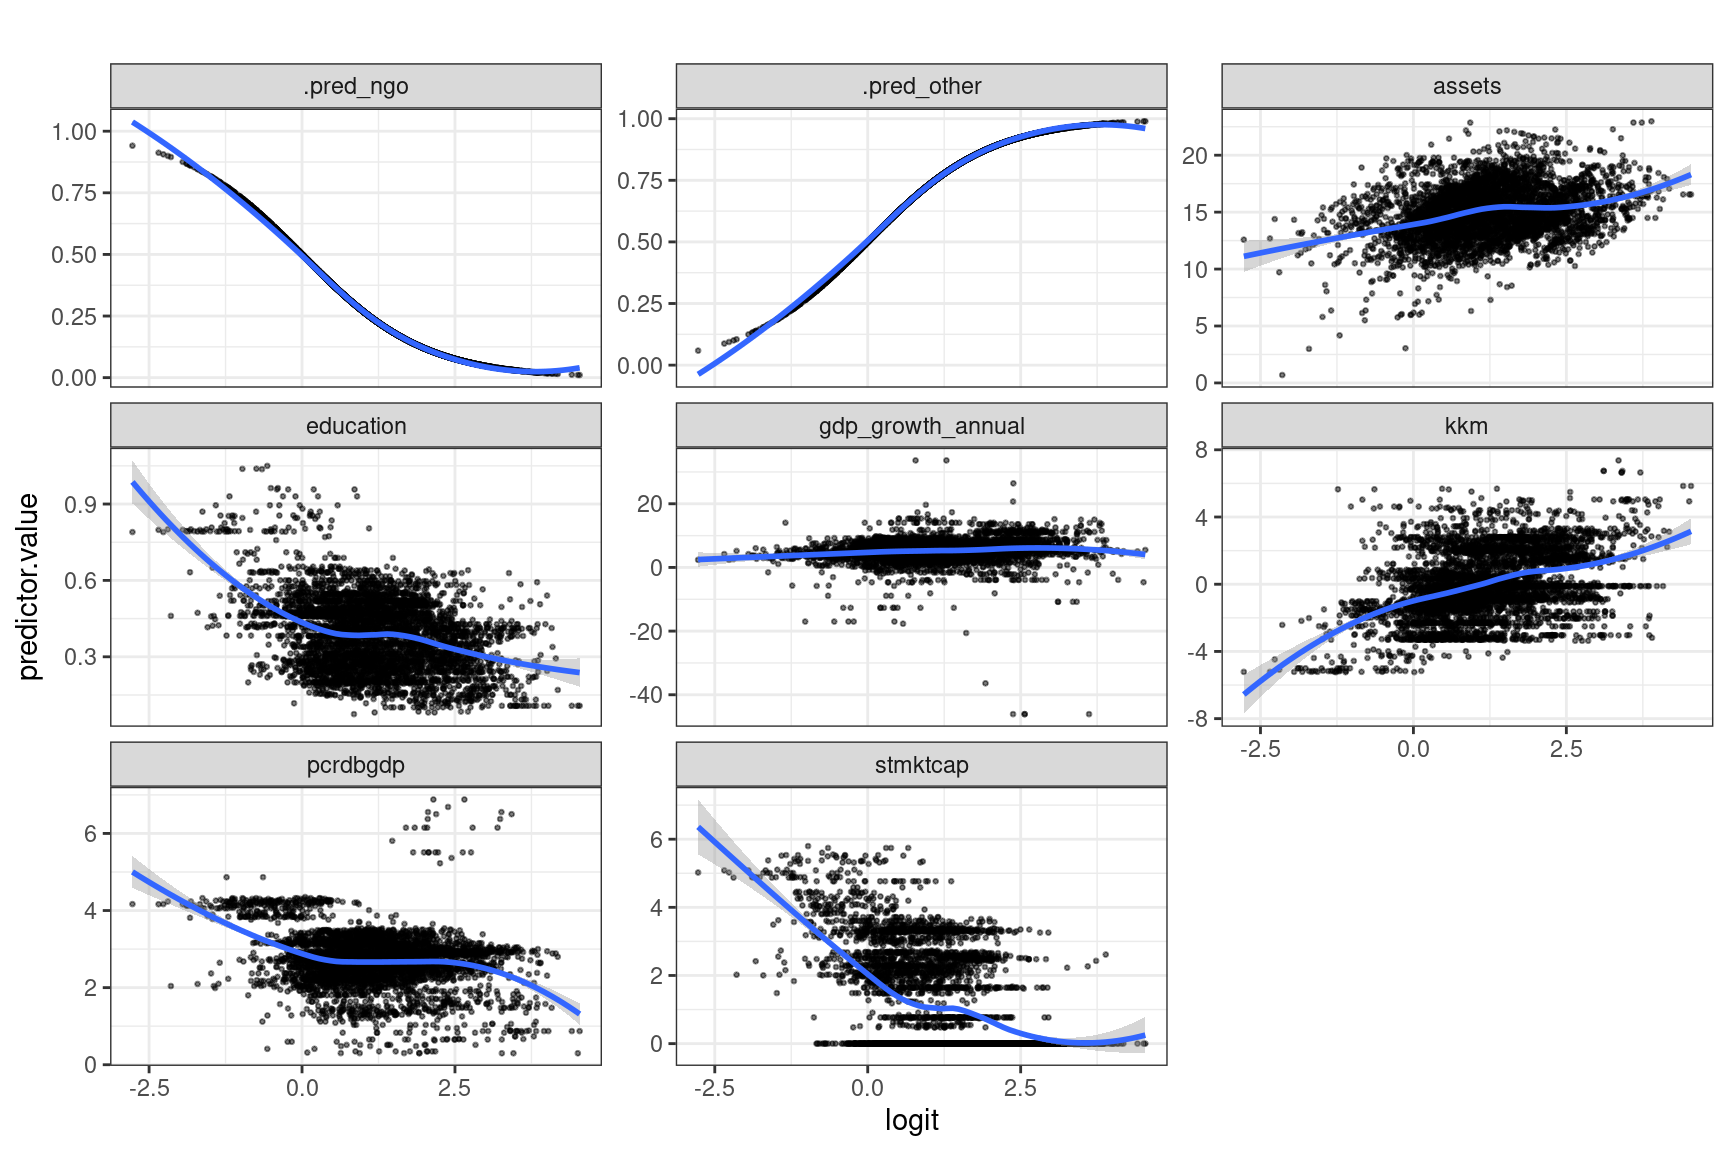
\includegraphics{_main_files/figure-latex/unnamed-chunk-42-1.pdf}
\caption{\label{fig:unnamed-chunk-42}Linearity of Independent Variables}
\end{figure}

\end{landscape}

\hypertarget{other-robustness-checks}{%
\subsection{Other Robustness Checks}\label{other-robustness-checks}}

In many cases, it is unlikely that a credit union starts as an NGO, given that they primarily serve clients with a similar professional base and geographic background. For this reason, we run a regression, excluding cooperatives, with the results displayed in Appendix 1. The results remain robust in this case, noting that signs of the coefficients do not change.

\hypertarget{conclusion}{%
\section{Conclusion}\label{conclusion}}

This article examined the factors that drive the transformation of MFIs from the NGO, not-for-profit model to the commercial, for-profit model, focusing on Africa. The analysis shows that at the MFI level, there are three critical factors; age, legal tradition, and size matter. At the aggregate level, it is the country institutional quality and stock market capitalisation that matter. Specifically, older firms are most likely to follow the not-for-profit model, while newer firms are most likely commercial. We expect that older firms are better at attracting donations and subsidies and hence still follow the earlier tradition of microfinance as a welfare tool to aid the financially excluded \autocite{d2017ngos}. For legal tradition, MFIs in civil law countries are the least likely to follow the commercial model relative to those in common law countries. The results align with the finance and law literature, where civil law countries have weaker capital markets. Hence, MFIs have a market void to fill profitably, unlike in common law countries where mainstream markets already fill much of the gap, leaving relatively fewer profit opportunities \autocite{la2013law,schnyder2018twenty}. MFIs in countries following other legal traditions other than common law and civil law are most likely to follow the commercial model.

Turning to size, larger firms tend to adopt the commercial model compared to relatively younger firms. We expect that larger firms are better at attracting commercial capital courtesy of the goodwill and the collateral to pledge when seeking funds publicly. Institutional quality relates positively to adopting the commercial model at the country level, while stock market capitalisation has the opposite effect. Institutional quality affects the ease of contracting, contract enforcement, and property rights \autocite{claessens2003financial}. Private credit to GDP and GDP growth rates are not significant drivers of the conversion of MFIs. However, the coefficients' signs indicate that private credit to GDP, like the stock market to GDP ratio, is inversely related to transformation probability. At the same time, GDP growth shows mixed effects, with significant positive coefficients.

\newpage

\hypertarget{appendices}{%
\section{Appendices}\label{appendices}}

\hypertarget{appendix-1-binary-models-excl.-cooperatives}{%
\subsection{Appendix 1: Binary Models (Excl. Cooperatives)}\label{appendix-1-binary-models-excl.-cooperatives}}

\begin{table}[!htbp] \centering 
  \caption{Models Excluding Cooperatives (Standard Errors in Brackets)} 
  \label{} 
\footnotesize 
\begin{tabular}{@{\extracolsep{5pt}}lcc} 
\\[-1.8ex]\hline 
\hline \\[-1.8ex] 
 & \multicolumn{2}{c}{\textit{Dependent variable:}} \\ 
\cline{2-3} 
\\[-1.8ex] & \multicolumn{2}{c}{Dummy: Current Legal Status} \\ 
\\[-1.8ex] & \textit{logistic} & \textit{probit} \\ 
\\[-1.8ex] & (1) & (2)\\ 
\hline \\[-1.8ex] 
 ageYoung & $-$0.747$^{***}$ & $-$0.421$^{***}$ \\ 
  & (0.114) & (0.065) \\ 
  & & \\ 
 ageMature & $-$1.200$^{***}$ & $-$0.691$^{***}$ \\ 
  & (0.106) & (0.060) \\ 
  & & \\ 
 legal\_traditionCivil & $-$0.421$^{***}$ & $-$0.239$^{***}$ \\ 
  & (0.117) & (0.068) \\ 
  & & \\ 
 legal\_traditionOther & 0.744$^{***}$ & 0.387$^{***}$ \\ 
  & (0.132) & (0.073) \\ 
  & & \\ 
 assets & 0.240$^{***}$ & 0.142$^{***}$ \\ 
  & (0.019) & (0.011) \\ 
  & & \\ 
 kkm & 0.095$^{***}$ & 0.057$^{***}$ \\ 
  & (0.019) & (0.011) \\ 
  & & \\ 
 pcrdbgdp & $-$0.112 & $-$0.049 \\ 
  & (0.076) & (0.042) \\ 
  & & \\ 
 stmktcap & $-$0.327$^{***}$ & $-$0.190$^{***}$ \\ 
  & (0.038) & (0.022) \\ 
  & & \\ 
 gdp\_growth\_annual & 0.016 & 0.012$^{*}$ \\ 
  & (0.011) & (0.006) \\ 
  & & \\ 
 Constant & $-$2.030$^{***}$ & $-$1.260$^{***}$ \\ 
  & (0.446) & (0.266) \\ 
  & & \\ 
\hline \\[-1.8ex] 
Year Effects & Yes & Yes \\ 
Deviance & 664*** & 657*** \\ 
df & 29 & 29 \\ 
Data & No Credit Unions & No Credit Unions \\ 
Observations & 4,782 & 4,782 \\ 
Log Likelihood & $-$2,439.000 & $-$2,446.000 \\ 
Akaike Inf. Crit. & 4,939.000 & 4,952.000 \\ 
\hline 
\hline \\[-1.8ex] 
\textit{Note:}  & \multicolumn{2}{l}{$^{*}$p$<$0.1; $^{**}$p$<$0.05; $^{***}$p$<$0.01} \\ 
\end{tabular} 
\end{table}

\newpage

\hypertarget{appendix-2-multinomial-logit-model--full-dataset}{%
\subsection{Appendix 2: Multinomial Logit Model- Full Dataset}\label{appendix-2-multinomial-logit-model--full-dataset}}

\begin{table}[!htbp] \centering 
  \caption{Multinomial Logit Model- Full Data (Standard Errors in Brackets)} 
  \label{} 
\footnotesize 
\begin{tabular}{@{\extracolsep{5pt}}lcccc} 
\\[-1.8ex]\hline 
\hline \\[-1.8ex] 
 & \multicolumn{4}{c}{\textit{Dependent variable:}} \\ 
\cline{2-5} 
\\[-1.8ex] & Dummy: Current Legal Status & NBFI & Coop & Rural Bank \\ 
\\[-1.8ex] & (1) & (2) & (3) & (4)\\ 
\hline \\[-1.8ex] 
 ageYoung & $-$1.640$^{***}$ & $-$0.621$^{***}$ & $-$0.543$^{***}$ & $-$0.973$^{***}$ \\ 
  & (0.184) & (0.133) & (0.139) & (0.374) \\ 
  & & & & \\ 
 ageMature & $-$2.650$^{***}$ & $-$1.460$^{***}$ & $-$0.630$^{***}$ & $-$0.840$^{***}$ \\ 
  & (0.174) & (0.128) & (0.128) & (0.294) \\ 
  & & & & \\ 
 legal\_traditionCivil & $-$3.750$^{***}$ & $-$1.190$^{***}$ & 1.890$^{***}$ & $-$5.130$^{***}$ \\ 
  & (0.266) & (0.143) & (0.167) & (1.070) \\ 
  & & & & \\ 
 legal\_traditionOther & $-$0.377$^{*}$ & 0.715$^{***}$ & 2.400$^{***}$ & $-$5.880$^{***}$ \\ 
  & (0.199) & (0.149) & (0.177) & (1.750) \\ 
  & & & & \\ 
 assets & 0.798$^{***}$ & 0.360$^{***}$ & $-$0.007 & 0.420$^{***}$ \\ 
  & (0.038) & (0.026) & (0.024) & (0.070) \\ 
  & & & & \\ 
 kkm & 0.450$^{***}$ & 0.250$^{***}$ & $-$0.066$^{**}$ & $-$1.480$^{***}$ \\ 
  & (0.034) & (0.024) & (0.026) & (0.185) \\ 
  & & & & \\ 
 pcrdbgdp & $-$0.008 & $-$0.048 & $-$0.250$^{***}$ & $-$2.640$^{***}$ \\ 
  & (0.109) & (0.085) & (0.091) & (0.624) \\ 
  & & & & \\ 
 stmktcap & $-$0.266$^{***}$ & $-$0.217$^{***}$ & $-$0.364$^{***}$ & $-$1.300$^{***}$ \\ 
  & (0.061) & (0.045) & (0.049) & (0.314) \\ 
  & & & & \\ 
 gdp\_growth\_annual & 0.043$^{**}$ & 0.054$^{***}$ & $-$0.005 & 0.019 \\ 
  & (0.018) & (0.014) & (0.013) & (0.079) \\ 
  & & & & \\ 
 Constant & $-$11.400$^{***}$ & $-$4.580$^{***}$ & $-$1.250$^{**}$ & $-$3.840 \\ 
  & (0.973) & (0.577) & (0.594) & (3.310) \\ 
  & & & & \\ 
\hline \\[-1.8ex] 
Year Effects & Yes & Yes & Yes & Yes \\ 
Data & Full & Full & Full & Full \\ 
Akaike Inf. Crit. & 10,124.000 & 10,124.000 & 10,124.000 & 10,124.000 \\ 
\hline 
\hline \\[-1.8ex] 
\textit{Note:}  & \multicolumn{4}{l}{$^{*}$p$<$0.1; $^{**}$p$<$0.05; $^{***}$p$<$0.01} \\ 
\end{tabular} 
\end{table}

\newpage

\hypertarget{appendix-3-multinomial-logit-model--full-data-excluding-credit-unions-cooperatives}{%
\subsection{Appendix 3: Multinomial Logit Model- Full Data Excluding Credit Unions/ Cooperatives}\label{appendix-3-multinomial-logit-model--full-data-excluding-credit-unions-cooperatives}}

\begin{table}[!htbp] \centering 
  \caption{Multinomial Logit Model- Full Data Without Cooperatives (Standard Errors in Brackets)} 
  \label{} 
\footnotesize 
\begin{tabular}{@{\extracolsep{5pt}}lcccc} 
\\[-1.8ex]\hline 
\hline \\[-1.8ex] 
 & \multicolumn{4}{c}{\textit{Dependent variable:}} \\ 
\cline{2-5} 
\\[-1.8ex] & Dummy: Current Legal Status & NBFI & Coop & Rural Bank \\ 
\\[-1.8ex] & (1) & (2) & (3) & (4)\\ 
\hline \\[-1.8ex] 
 ageYoung & $-$1.640$^{***}$ & $-$0.621$^{***}$ & $-$0.543$^{***}$ & $-$0.973$^{***}$ \\ 
  & (0.184) & (0.133) & (0.139) & (0.374) \\ 
  & & & & \\ 
 ageMature & $-$2.650$^{***}$ & $-$1.460$^{***}$ & $-$0.630$^{***}$ & $-$0.840$^{***}$ \\ 
  & (0.174) & (0.128) & (0.128) & (0.294) \\ 
  & & & & \\ 
 legal\_traditionCivil & $-$3.750$^{***}$ & $-$1.190$^{***}$ & 1.890$^{***}$ & $-$5.130$^{***}$ \\ 
  & (0.266) & (0.143) & (0.167) & (1.070) \\ 
  & & & & \\ 
 legal\_traditionOther & $-$0.377$^{*}$ & 0.715$^{***}$ & 2.400$^{***}$ & $-$5.880$^{***}$ \\ 
  & (0.199) & (0.149) & (0.177) & (1.750) \\ 
  & & & & \\ 
 assets & 0.798$^{***}$ & 0.360$^{***}$ & $-$0.007 & 0.420$^{***}$ \\ 
  & (0.038) & (0.026) & (0.024) & (0.070) \\ 
  & & & & \\ 
 kkm & 0.450$^{***}$ & 0.250$^{***}$ & $-$0.066$^{**}$ & $-$1.480$^{***}$ \\ 
  & (0.034) & (0.024) & (0.026) & (0.185) \\ 
  & & & & \\ 
 pcrdbgdp & $-$0.008 & $-$0.048 & $-$0.250$^{***}$ & $-$2.640$^{***}$ \\ 
  & (0.109) & (0.085) & (0.091) & (0.624) \\ 
  & & & & \\ 
 stmktcap & $-$0.266$^{***}$ & $-$0.217$^{***}$ & $-$0.364$^{***}$ & $-$1.300$^{***}$ \\ 
  & (0.061) & (0.045) & (0.049) & (0.314) \\ 
  & & & & \\ 
 gdp\_growth\_annual & 0.043$^{**}$ & 0.054$^{***}$ & $-$0.005 & 0.019 \\ 
  & (0.018) & (0.014) & (0.013) & (0.079) \\ 
  & & & & \\ 
 Constant & $-$11.400$^{***}$ & $-$4.580$^{***}$ & $-$1.250$^{**}$ & $-$3.840 \\ 
  & (0.973) & (0.577) & (0.594) & (3.310) \\ 
  & & & & \\ 
\hline \\[-1.8ex] 
Year Effects & Yes & Yes & Yes & Yes \\ 
Data & Full & Full & Full & Full \\ 
Akaike Inf. Crit. & 10,124.000 & 10,124.000 & 10,124.000 & 10,124.000 \\ 
\hline 
\hline \\[-1.8ex] 
\textit{Note:}  & \multicolumn{4}{l}{$^{*}$p$<$0.1; $^{**}$p$<$0.05; $^{***}$p$<$0.01} \\ 
\end{tabular} 
\end{table}

\newpage

\hypertarget{appendix-4-multinomial-logit-model-with-full-dataset-but-no-year-effects}{%
\subsection{Appendix 4: Multinomial Logit Model With Full Dataset But No Year Effects}\label{appendix-4-multinomial-logit-model-with-full-dataset-but-no-year-effects}}

\begin{table}[!htbp] \centering 
  \caption{Multinomial Logit Model- Full Data Without Year Effects (Standard Errors in Brackets)} 
  \label{} 
\footnotesize 
\begin{tabular}{@{\extracolsep{5pt}}lcccc} 
\\[-1.8ex]\hline 
\hline \\[-1.8ex] 
 & \multicolumn{4}{c}{\textit{Dependent variable:}} \\ 
\cline{2-5} 
\\[-1.8ex] & Dummy: Current Legal Status & NBFI & Coop & Rural Bank \\ 
\\[-1.8ex] & (1) & (2) & (3) & (4)\\ 
\hline \\[-1.8ex] 
 ageYoung & $-$1.740$^{***}$ & $-$0.619$^{***}$ & $-$0.543$^{***}$ & $-$1.120$^{***}$ \\ 
  & (0.181) & (0.132) & (0.136) & (0.359) \\ 
  & & & & \\ 
 ageMature & $-$2.620$^{***}$ & $-$1.400$^{***}$ & $-$0.539$^{***}$ & $-$0.822$^{***}$ \\ 
  & (0.170) & (0.126) & (0.125) & (0.284) \\ 
  & & & & \\ 
 legal\_traditionCivil & $-$3.830$^{***}$ & $-$1.290$^{***}$ & 1.700$^{***}$ & $-$5.380$^{***}$ \\ 
  & (0.264) & (0.140) & (0.163) & (1.110) \\ 
  & & & & \\ 
 legal\_traditionOther & $-$0.359$^{*}$ & 0.720$^{***}$ & 2.390$^{***}$ & $-$11.000$^{***}$ \\ 
  & (0.195) & (0.146) & (0.175) & (0.0004) \\ 
  & & & & \\ 
 assets & 0.787$^{***}$ & 0.373$^{***}$ & $-$0.006 & 0.346$^{***}$ \\ 
  & (0.036) & (0.025) & (0.023) & (0.061) \\ 
  & & & & \\ 
 kkm & 0.471$^{***}$ & 0.260$^{***}$ & $-$0.044$^{*}$ & $-$1.420$^{***}$ \\ 
  & (0.033) & (0.024) & (0.025) & (0.138) \\ 
  & & & & \\ 
 pcrdbgdp & 0.156 & 0.081 & 0.001 & $-$2.300$^{***}$ \\ 
  & (0.102) & (0.080) & (0.082) & (0.371) \\ 
  & & & & \\ 
 stmktcap & $-$0.269$^{***}$ & $-$0.248$^{***}$ & $-$0.431$^{***}$ & $-$1.110$^{***}$ \\ 
  & (0.060) & (0.044) & (0.047) & (0.239) \\ 
  & & & & \\ 
 gdp\_growth\_annual & 0.057$^{***}$ & 0.061$^{***}$ & $-$0.0003 & $-$0.027 \\ 
  & (0.016) & (0.013) & (0.012) & (0.039) \\ 
  & & & & \\ 
 Constant & $-$10.700$^{***}$ & $-$4.540$^{***}$ & $-$0.470 & $-$0.495 \\ 
  & (0.558) & (0.371) & (0.349) & (1.010) \\ 
  & & & & \\ 
\hline \\[-1.8ex] 
Year Effects & Yes & No & No & No \\ 
Data & No Coop & No Coop & No Coop & No Coop \\ 
Akaike Inf. Crit. & 10,187.000 & 10,187.000 & 10,187.000 & 10,187.000 \\ 
\hline 
\hline \\[-1.8ex] 
\textit{Note:}  & \multicolumn{4}{l}{$^{*}$p$<$0.1; $^{**}$p$<$0.05; $^{***}$p$<$0.01} \\ 
\end{tabular} 
\end{table}

\newpage

\hypertarget{appendix-5-multinomial-logit-model--full-data-excluding-credit-unions-cooperatives-and-year-effects}{%
\subsection{Appendix 5: Multinomial Logit Model- Full Data Excluding Credit Unions/ Cooperatives and Year Effects}\label{appendix-5-multinomial-logit-model--full-data-excluding-credit-unions-cooperatives-and-year-effects}}

\begin{table}[!htbp] \centering 
  \caption{Multinomial Logit Model- Full Data Excluding Cooperatives and Year Effects (Standard Errors in Brackets)} 
  \label{} 
\footnotesize 
\begin{tabular}{@{\extracolsep{5pt}}lcccc} 
\\[-1.8ex]\hline 
\hline \\[-1.8ex] 
 & \multicolumn{4}{c}{\textit{Dependent variable:}} \\ 
\cline{2-5} 
\\[-1.8ex] & Dummy: Current Legal Status & NBFI & Coop & Rural Bank \\ 
\\[-1.8ex] & (1) & (2) & (3) & (4)\\ 
\hline \\[-1.8ex] 
 ageYoung & $-$1.740$^{***}$ & $-$0.619$^{***}$ & $-$0.543$^{***}$ & $-$1.120$^{***}$ \\ 
  & (0.181) & (0.132) & (0.136) & (0.359) \\ 
  & & & & \\ 
 ageMature & $-$2.620$^{***}$ & $-$1.400$^{***}$ & $-$0.539$^{***}$ & $-$0.822$^{***}$ \\ 
  & (0.170) & (0.126) & (0.125) & (0.284) \\ 
  & & & & \\ 
 legal\_traditionCivil & $-$3.830$^{***}$ & $-$1.290$^{***}$ & 1.700$^{***}$ & $-$5.380$^{***}$ \\ 
  & (0.264) & (0.140) & (0.163) & (1.110) \\ 
  & & & & \\ 
 legal\_traditionOther & $-$0.359$^{*}$ & 0.720$^{***}$ & 2.390$^{***}$ & $-$11.000$^{***}$ \\ 
  & (0.195) & (0.146) & (0.175) & (0.0004) \\ 
  & & & & \\ 
 assets & 0.787$^{***}$ & 0.373$^{***}$ & $-$0.006 & 0.346$^{***}$ \\ 
  & (0.036) & (0.025) & (0.023) & (0.061) \\ 
  & & & & \\ 
 kkm & 0.471$^{***}$ & 0.260$^{***}$ & $-$0.044$^{*}$ & $-$1.420$^{***}$ \\ 
  & (0.033) & (0.024) & (0.025) & (0.138) \\ 
  & & & & \\ 
 pcrdbgdp & 0.156 & 0.081 & 0.001 & $-$2.300$^{***}$ \\ 
  & (0.102) & (0.080) & (0.082) & (0.371) \\ 
  & & & & \\ 
 stmktcap & $-$0.269$^{***}$ & $-$0.248$^{***}$ & $-$0.431$^{***}$ & $-$1.110$^{***}$ \\ 
  & (0.060) & (0.044) & (0.047) & (0.239) \\ 
  & & & & \\ 
 gdp\_growth\_annual & 0.057$^{***}$ & 0.061$^{***}$ & $-$0.0003 & $-$0.027 \\ 
  & (0.016) & (0.013) & (0.012) & (0.039) \\ 
  & & & & \\ 
 Constant & $-$10.700$^{***}$ & $-$4.540$^{***}$ & $-$0.470 & $-$0.495 \\ 
  & (0.558) & (0.371) & (0.349) & (1.010) \\ 
  & & & & \\ 
\hline \\[-1.8ex] 
Year Effects & No & No & No & No \\ 
Data & Full & Full & Full & Full \\ 
Akaike Inf. Crit. & 10,187.000 & 10,187.000 & 10,187.000 & 10,187.000 \\ 
\hline 
\hline \\[-1.8ex] 
\textit{Note:}  & \multicolumn{4}{l}{$^{*}$p$<$0.1; $^{**}$p$<$0.05; $^{***}$p$<$0.01} \\ 
\end{tabular} 
\end{table}

\newpage

\hypertarget{appendix-6-legal-traditions-in-africa}{%
\subsection{Appendix 6: Legal Traditions in Africa}\label{appendix-6-legal-traditions-in-africa}}

\begin{table}
\caption{\label{tab:unnamed-chunk-48}Legal Traditions in Africa}

\centering
\begin{tabular}[t]{l}
\toprule
Common\_Law\\
\midrule
Botswana\\
Gambia, The\\
Ghana\\
Kenya\\
Lesotho\\
\addlinespace
Liberia\\
Malawi\\
Namibia\\
Nigeria\\
Sierra Leone\\
\addlinespace
South Africa\\
South Sudan\\
Sudan\\
Eswatini\\
Tanzania\\
\addlinespace
Uganda\\
Zambia\\
Zimbabwe\\
\bottomrule
\end{tabular}
\centering
\begin{tabular}[t]{l}
\toprule
Civil\_Law\\
\midrule
Algeria\\
Benin\\
Burkina Faso\\
Cameroon\\
Central African Republic\\
\addlinespace
Chad\\
Comoros\\
Congo, Rep.\\
Cote d'Ivoire\\
Gabon\\
\addlinespace
Guinea\\
Madagascar\\
Mali\\
Mauritania\\
Morocco\\
\addlinespace
Niger\\
Senegal\\
Togo\\
Tunisia\\
\bottomrule
\end{tabular}
\centering
\begin{tabular}[t]{l}
\toprule
Other\_Law\\
\midrule
Equatorial Guinea\\
Angola\\
Burundi\\
Cape Verde\\
Congo, Dem. Rep.\\
\addlinespace
Egypt, Arab Republic of\\
Ethiopia\\
Eritrea\\
Guinea-Bissau\\
Mozambique\\
\addlinespace
Rwanda\\
\bottomrule
\end{tabular}
\end{table}

\begin{savequote}
``No end to poverty without financial inclusion.''
\qauthor{--- The World Bank.}\end{savequote}



\hypertarget{transformation-of-microfinance-institutions-and-its-effects-on-financial-inclusion-in-africa}{%
\chapter{Transformation of Microfinance Institutions and its Effects on Financial Inclusion in Africa}\label{transformation-of-microfinance-institutions-and-its-effects-on-financial-inclusion-in-africa}}

\chaptermark{MFI Transformation and Financial Inclusion}

\minitoc 

\newpage

\begin{center}

\textbf{ABSTRACT}

\end{center}

\begin{quote}
The shift away from the not-for-profit, non-governmental organisations microfinance institutions (NGO-MFIs) model has seen the rise of commercial MFIs in forms such as commercial banks, credit unions, and rural banks. The shift arose partly due to neo-liberalism and the need for MFIs to reach the financially excluded more sustainably than had hitherto been the case. Therefore, this article examines how the shift has affected financial inclusion in Africa, utilising data from the Microfinance Information Exchange (MIX). Our results show that the transformation from the NGO model to the commercial models could negatively affect the depth of financial outreach, especially given that NGOs characteristically have better outreach to women and advance smaller denomination loans on average. We also find that NGOs have higher median gross loans than other legal forms of MFIs except cooperatives, although commercial banks have the highest average gross loans. These results remain robust upon removing outliers and controlling for factors that affect the ability of MFIs to offer financial services to the poor.
\end{quote}

\vspace{10mm}

\textbf{Key Words}: Microfinance, Transformation, Financial Inclusion, Africa

\vspace{5mm}

\textbf{JEL Classification}: G210, G230

\newpage

\newpage

\hypertarget{background-1}{%
\section{Background}\label{background-1}}

In 1992, PRODEM, a micro-finance institution (MFI) in Bolivia, converted from a non-governmental organisation (NGO) to a commercial bank, BANCOSOL. In fact, in the immediate past three decades, numerous NGO MFIs across the globe have adopted the commercial forms of microfinance (Table 3.1). In this article, we examine how the conversion of MFIs to the commercial model affects financial inclusion in terms of the depth and breadth of outreach to the financially excluded. Depth refers to the extent of the traditional financially excluded clients reached by MFIs. If an MFI serves more financially excluded people like women and the poor, it has deeper outreach \^{}{[}The quotation at the start of the chapter is available at \textcite{financialtimesinclusion}.

On the other hand, breadth refers to the sheer number of clients reached regardless of their level of financial exclusion. Thus, an MFI that offers more loans to many people has more breadth of outreach. In other words, we explore how the transformation of MFIs typically drives their average loan balance per borrower, the proportion of women borrowers and gross loans. The former two metrics capture depth while the latter proxies breadth.

The study focuses on Africa, a continent that is the epicentre of financial exclusion despite remarkable economic progress of the last three decades \autocite{beck2014sme,allen2011african}. Evaluating the effects of transformation by using global metrics is likely to mask regional heterogeneity, given that these effects could manifest differently in varying settings \autocite{d2017ngos,d2013unsubsidized} \footnote{The MIX Market database is available on this link \url{https://datacatalog.worldbank.org/dataset/mix-market}.}.

Most pioneer microfinance institutions adopted a not-for-profit model \autocite{dichter1996questioning}, operating mainly as non-governmental organisations (NGOs). However, the dominance of neo-liberalism in organising production has seen many donors scale back and push MFIs to strive for financial sustainability \autocite{bateman2010doesn}. The arguments for the commercial approach to running microfinance activities revolve around sustainability. The financial sustainability school posits that MFIs can best serve the financially excluded when they have a degree of financial self-sufficiency \autocite{kodongo2013individual}. For instance, profit-oriented MFIs could offer financial services to the relatively well-off at market rates and use the proceeds (profits) to subsidise services to the poor more than relying on donations and subsidies alone. Hence, MFIs pursuing the for-profit model may experience mission expansion \autocite{mersland2010microfinance,louis2013financial}. Also, donor funds are volatile and subject to political and economic conditions \autocite{garmaise2013cheap,d2017aid}. In this respect, a substantial body of research finds that the transformation of microfinance institutions enhances outreach to the financially excluded \autocite{frank2008stemming,gutierrez2009social,mersland2010microfinance,quayes2012depth,mia2017mission,d2013unsubsidized}.

The proponents of MFI transformation point to the concerning possibility of mission drift. Mission drift happens when MFIs focus less on providing financial services to the financially excluded in favour of making profits. Some researchers have found this to be the case \autocite{louis2013financial,bos2015practice,d2013unsubsidized,hartarska2012governance}. Two theories can be said to underpin the MFI transformation phenomenon. The first is the agency theory on the conflicts between providers of capital and managers. In a quest to minimise agency conflicts, managers may consciously or sub-consciously place less emphasis on the social mission of MFIs, reaching out to the financially excluded. Instead, managers may more overtly focus on pursuing financial returns for shareholders and debt-holders, thus causing mission drift. The theory presumes that the motivation for all fund providers is financial returns, which is not always the case.

The second one, the institutional theory, examines the rise, persistence and decline of institutional structures over time. The central question here is; What drives the adoption and fall of certain institutional norms \autocite{powell2012new}? In this respect, some institutionalists claim that prevailing institutional culture is more potent than market forces in driving the adoption or rejection of emergent institutional structures. Institutionalists posit that one of the drivers is coercion. In the case of MFIs, some donors have put implicit or explicit pressure on financial sustainability.

Additionally, the adoption of institutional norms in most cases arises out of the need to fit into the institutional environment. The desire to be compliant may explain the prevalence of NGOs not-for-profit type MFIs in the early years of the microfinance paradigm and the trend towards the transformation of MFIs to commercial entities that is now ongoing. Notably, institutional theory sheds light on the dilemmas managers face when institutional norms change \autocite{thornton2015institutional}. For instance, how can managers of MFIs reconcile financial sustainability with the original priority of outreach to the financially excluded?

\begin{table}

\caption{\label{tab:unnamed-chunk-51}Sample of Transformed MFIs}
\centering
\fontsize{9}{11}\selectfont
\begin{tabular}[t]{llll}
\toprule
Institution & Country & Year & Converted\_to\\
\midrule
Finansol & Colombia & 1993 & Commercial Finance Company\\
OIBM & Malawi & 2002 & NBFI\\
PRIDE & Tanzania & 2009 & NBFI\\
Kenya Women Finance Trust & Kenya & 2010 & NBFI\\
Faulu & Kenya & 2010 & NBFI\\
\addlinespace
OI-SASL & Ghana & 2013 & NBFI\\
\bottomrule
\multicolumn{4}{l}{\rule{0pt}{1em}Source: Authors' construction from the literature}\\
\multicolumn{4}{l}{\rule{0pt}{1em}\textit{Note: }}\\
\multicolumn{4}{l}{\rule{0pt}{1em}\textsuperscript{1} This is a snapshot of the many MFIs that have converted over the years accross the globe}\\
\end{tabular}
\end{table}

As noted earlier, research outcomes on the effects of the transformation of microfinance institutions are mixed. \textcite{morduch2019challenges} argue that if commercial MFIs could sustainably achieve financial sustainability while also reaching the poor, NGOs would not exist. In that context, therefore, the most critical question relates to how the transformation of MFIs would affect their core mission of providing financial services to the financially excluded. The issue is vital due to the legitimacy that MFIs derive from serving the financially excluded. Besides, financial inclusion is central to alleviating poverty and achieving inclusive growth, an essential dimension of financial development. In this article, we use data from the Microfinance Information Exchange (MIX) to evaluate the ways that the transformation of MFIs affects financial inclusion in Africa.

We capture the extent of financial inclusion in Africa by using three metrics:

\begin{itemize}
\tightlist
\item
  The percentage of female borrowers.
\item
  Average loan balance per borrower.
\item
  The ratio of the gross loan portfolio to total assets of each MFI \autocite{d2017ngos}.
\end{itemize}

The first two metrics proxy the depth of outreach, with more significant outreach to women indicating deeper outreach, given that women form a substantial proportion of the financially excluded population in Africa \autocite{ayyagari2013financing}. A higher average loan balance per borrower, on the other hand, corresponds to a lower depth of outreach to any group of the financially excluded. The presumption is that financially excluded people usually borrow in smaller denominations that have drawn reservations from some researchers who argue poor people could progressively demand bigger loans as they get better off. Also, MFIs regularly use progressive lending where people who successfully pay off loans qualify for larger loan amounts. Finally, gross loans to assets capture the breadth of outreach, with higher ratios indicating more breadth.

We have organised the rest of the article as follows. Section 1.1 highlights the results of the study. In section 2, we review the background literature on MFI transformation. In section 3, we describe the methodology and, in section 4, we present and discuss the results and close with concluding remarks in section 5.

\hypertarget{summary-of-results-1}{%
\subsection{Summary of Results}\label{summary-of-results-1}}

Overall, we find that the conversion away from the NGO, not-for-profit model in Africa is harmful to financial inclusion's depth and breadth. NGO-type MFIs consistently outperform the commercial-oriented MFIs regarding the outreach to women borrowers. Additionally, NGO-type MFIs have the lowest average loan balance per borrower, indicating that they reach out to the poorest and, presumably, more financially excluded people. Turning to the ratio of gross loans to assets, NGO-type MFIs come second to credit unions/ cooperatives, thus indicating that breadth and depth of outreach are not necessarily mutually exclusive. Further examination of the trend suggests that profit-oriented MFIs reflect a measure of mission drift.

On the one hand, serving poor, financially excluded people is costly, which hurts the profitability of MFIs. On the other hand, profit orientation implies commercial capital, interest expense on debt capital and dividends on equity capital. If it is hard to reconcile these two objectives, we are inclined to back the literature that opposes the commercialisation of MFIs. As we shall see later, it seems odd that NGO-type MFIs lend more gross loans (breadth) than most commercial-oriented MFIs, though it turns out that both cooperatives and NGO-type MFIs hold the lowest volume of assets relative to other legal types. Furthermore, the other important drivers of financial inclusion are the age of MFI, operating expense to assets ratio, donations to assets ratio, capital to assets ratio, asset structure, size, education and profit margin. In the next section, we highlight the methodology and then go to the details of the results.

\hypertarget{theory-and-empirical-literature}{%
\section{Theory and Empirical Literature}\label{theory-and-empirical-literature}}

The extent to which the transformation of MFIs affects financial inclusion has been the subject of substantial research. However, there is a lack of consensus on the outcomes about its effects. Theories underlying aspects of the transformation of MFIs are the agency theory \autocite{jensen1976theory} and institutional theory \autocite{powell2012new}. Agency theory, in this case, implies that injection of commercial capital, a consequence of transformation, is likely to motivate managers to target financial return at the expense of social return to satisfy shareholders and debt-holders, the conventional providers of commercial capital. From this perspective, transformation implies that mission drift is inevitable. Indeed, \textcite{morduch2019challenges} argue that if mission drift is not an issue in microfinance, then the NGOs MFI model would not exist, meaning that NGOs (not-for-profit) MFIs exist to fill a gap left by commercial MFIs.

The institutionalists weigh how specific organisational structures dominate and ultimately decline and get discarded \autocite{powell2012new}. Institutionalists note that in certain situations, people adopt given structures without critical scrutiny to fit into the prevailing institutional environment merely. This argument could partly explain the prevalence of NGO MFI models at the early stages of microfinance evolution and the current rise of MFI commercialisation. However, the pressure to change takes several forms, with the most notable one being coercive pressure, where stakeholders put forth overt or covert pressure for MFIs to convert. In the case of MFIs, the pressure to adopt a commercial model came with the rise of neo-liberal thought around production and its funding \autocite{bateman2010doesn}, with major donors like USAID signalling their expectation that MFIs should become more financially sustainable going forward \autocite{d2013unsubsidized}. The problem for MFIs that transform is how best to balance between social goals of reaching the poor and the commercial goals that come with commercial capital and the attendant decline of donor funding.

\textcite{thornton2002rise} and \textcite{thornton2015institutional} note that ``the meaning and legitimacy of various sources of organisational identity, strategy and structure are shaped by a prevailing institutional logic''. The management of transformed MFIs can identify with microfinance as a social pursuit by emphasising social goals over profits. Alternatively, they may view microfinance as a financial venture by placing profits over social outreach. The former corresponds to the welfare model of microfinance, which posits that the social mission of microfinance is incompatible with the profit motive. The latter is the financial sustainability model, which views financial returns as a precondition for the sustainable pursuit of financial services goals of reaching the financially excluded. A third model, the win-win approach, attempts to reconcile the welfare and sustainability approach by proposing that financial and social performance are not always substituting but complementary. Different researchers have availed evidence in support of either school, as described next.

As noted, support for MFI transformation rests on two primary grounds. First, donations are subject to social, economic, and political conditions \autocite{garmaise2013cheap,armendariz2013subsidy,d2017aid}. Consequently, some researchers argue that microfinance can only be sustainable if MFIs have a level of financial self-sufficiency. In this regard, these scholars note that MFIs could advance financial services to the financially well-off and use the proceeds (profits) to reach more financially excluded people at subsidised rates, which would then lead to ``mission expansion'' as opposed to ``mission drift''. \textcite{frank2008stemming} provides empirical support for these arguments noting that transformed MFIs score higher in terms of client outreach and the number of female clients reached, although the proportion of female clients reached declines. They also find that transformed MFIs record higher growth in gross loan portfolio with better product diversification.

Similarly, \textcite{d2017ngos} finds that transformed MFIs charge a lower interest rate to micro-borrowers. \textcite{louis2013financial}, using self-organising maps and k-means clustering, find a positive relationship between financial sustainability and social performance to imply that steps to enhance financial sustainability are good. Other researchers that have found a positive link between financial and social efficiency include \textcite{gutierrez2009social}, \textcite{mersland2010microfinance}, and \textcite{quayes2012depth}.

In contrast to the above findings, several researchers have found transformation to be harmful in terms of outreach to the financially excluded. For instance, \textcite{d2017ngos} find that although transformed MFIs charge lower interest and experience a drop in operating expenses, their average loan sizes increase, indicative of mission drift. \textcite{mia2017mission} also find a trade-off between depth of outreach and the profit motive of MFIs in Bangladesh using both static and dynamic panel data methods. \textcite{d2013unsubsidized} notes that MFIs with little or no subsidies exhibit more significant mission drift. In our case, NGOs have the highest donations, implying that they may show greater social inclination. For instance, firms in Africa and Asia compensate for low subsidies by charging higher interest rates, while Latin America serves fewer women. In Europe and Central Asia, the tendency is to serve fewer indigent clients. \textcite{bos2015practice} also notes that MFIs that stay close to their original mission are the most socially efficient, while those that attempt to pursue a double bottom line are relatively inefficient. Further, they note that not all MFIs suffer mission drift the same way, arguing that MFIs with high input-output efficiency may not experience mission drift at all.

Besides, \textcite{campion1999institutional} argue that the presence or absence of mission drift in a transformed MFI is a corporate governance issue and an outcome of the challenges of the scaling up of MF services. They argue that good corporate governance allows the management to balance between financial performance and outreach. It means that MFIs could address mission drift problems through proper corporate governance regardless of whether an MFI is an NGO or commercial-type entity. Moreover, \textcite{marti2016financial} argue that different social groups such as employees, management, and MFI clients are likely to have different views, including varying definitions of social welfare. Thus, the presence or absence of mission drift may not arise from deliberate management decisions but instead from conflicting viewpoints on the meaning of social welfare between stakeholders. Given the conflicting evidence and varying views regarding mission drift in MFIs, the arguments by \textcite{morduch1999microfinance} and \textcite{morduch2000microfinance} that the microfinance industry should accommodate different legal forms of MFIs to serve different clients' needs appear to be valid.

\hypertarget{method-1}{%
\section{Method}\label{method-1}}

We run fixed and random effects models based on the results of the Hausmann Tests (see Appendix 1). The design of fixed effects models allows for the study of the causes of changes within an entity. It accomplishes this by controlling for all time-invariant differences between the individuals, so the estimated coefficients of the fixed-effects models cannot be biased because of omitted time-invariant characteristics, such as culture \autocite{torres2007panel}. On the other hand, Random effect models assist in controlling for unobserved heterogeneity when the heterogeneity is constant over time and uncorrelated with the explanatory variables. Following \textcite{roberts2013endogeneity}, we fit the following model.

\begin{equation}
y_{it} = \hat{a} + \hat{b}x_{it} + \mu_{it}
\end{equation}

In this case, \(y_{it}\) is the independent variable; interchangeably represented by per cent of female borrowers, average loan balance per borrower, and gross loan portfolio to total assets. The first two metrics capture financial depth, while gross loans capture the breadth of outreach.

Also, \(x_{it}\) is a matrix of independent variables. The variable of interest in our case is the current legal form of the MFI, which enters the model as a dummy representing NGOs, NBFIs, commercial banks, rural banks and credit unions/ cooperatives \autocite{ayyagari2013financing}. The other control variables include age dummy, a dummy for region, operating expenses to assets ratio, donations to assets ratio, equity capital to assets ratio, asset structure, size (logarithm of total assets), education, and profit margin all of which are derived from the literature \autocite{ayyagari2013financing,d2017ngos,d2013unsubsidized}.

Finally, \(\mu_{it}\) is the error term that we assume has zero mean conditional on \(x_{it}\).

Further,

\begin{equation}
\mu_{it} = c_{i} + \varepsilon_{it}
\end{equation}

In the equation, \(c_{i}\) captures the aggregate effects of the unobserved, time-invariant explanatory variables for \(y_{it}\).

In the case where \(c_{i}\) and \(x_{it}\) are correlated, then \(c_{i}\) is a fixed effect, otherwise, it is a random effect. Note that the existence of fixed effects implies the presence of endogeneity. For random effects, on the other hand, endogeneity is not a concern. However, the random-effects model affects the computation of standard errors \autocite{roberts2013endogeneity}. To eliminate the fixed effect prone to endogeneity, we run the within estimator model \autocite{clark2015should}. We present the results from the estimation of the empirical model in the next section.

\hypertarget{results}{%
\section{Results}\label{results}}

In this section, we begin by visualizing the study variables followed by summary statistics of the variables. We then run and discuss the results of the regression model.

\hypertarget{exploratory-data-analysis-1}{%
\subsection{Exploratory Data Analysis}\label{exploratory-data-analysis-1}}

In this section, we explore the data by visualizing the pertinent variables and computing their summary statistics.

\hypertarget{data-visualization}{%
\subsubsection{Data Visualization}\label{data-visualization}}

Figure 3.1 shows the correlation matrix and a graphical view of the relationships between the numeric variables. The highest level of correlation is between operating expense to assets ratio and donations to assets ratio, meaning that MFIs that receive more donations spend relatively more, which is suitable for financial inclusion. On the other hand, the relatively low correlations between the variables suggest that multicollinearity is not likely to be a significant concern for the regression analysis that we embark on later in the article. The main diagonal shows the distribution of the individual variables. In this case, there is high skewness exhibited by the donations to assets ratio, average loan balance per borrower and gross loans to assets ratio. It means that relatively few firms account for a considerable chunk of the donations received, in this case among NGOs, cooperatives and NBFIs. The highest correlation exists between the operating expenses to assets ratio and donations to assets ratio, meaning that donor-funded MFIs have more operating costs probably because they are less constrained by profit/ interest seeking shareholders and debt holders. This observation may imply that if it is expensive to administer and monitor small loans, then the profit-oriented model is not suitable for financial inclusion as it constrains spending. The summary statistics in Tables 3.2, 3.3, and 3.4 that follow highlight the discussed issues but offer a more comprehensive array of statistical measures, including the mean, standard deviation and quantiles.

\newpage
\begin{landscape}

\begin{figure}
\centering
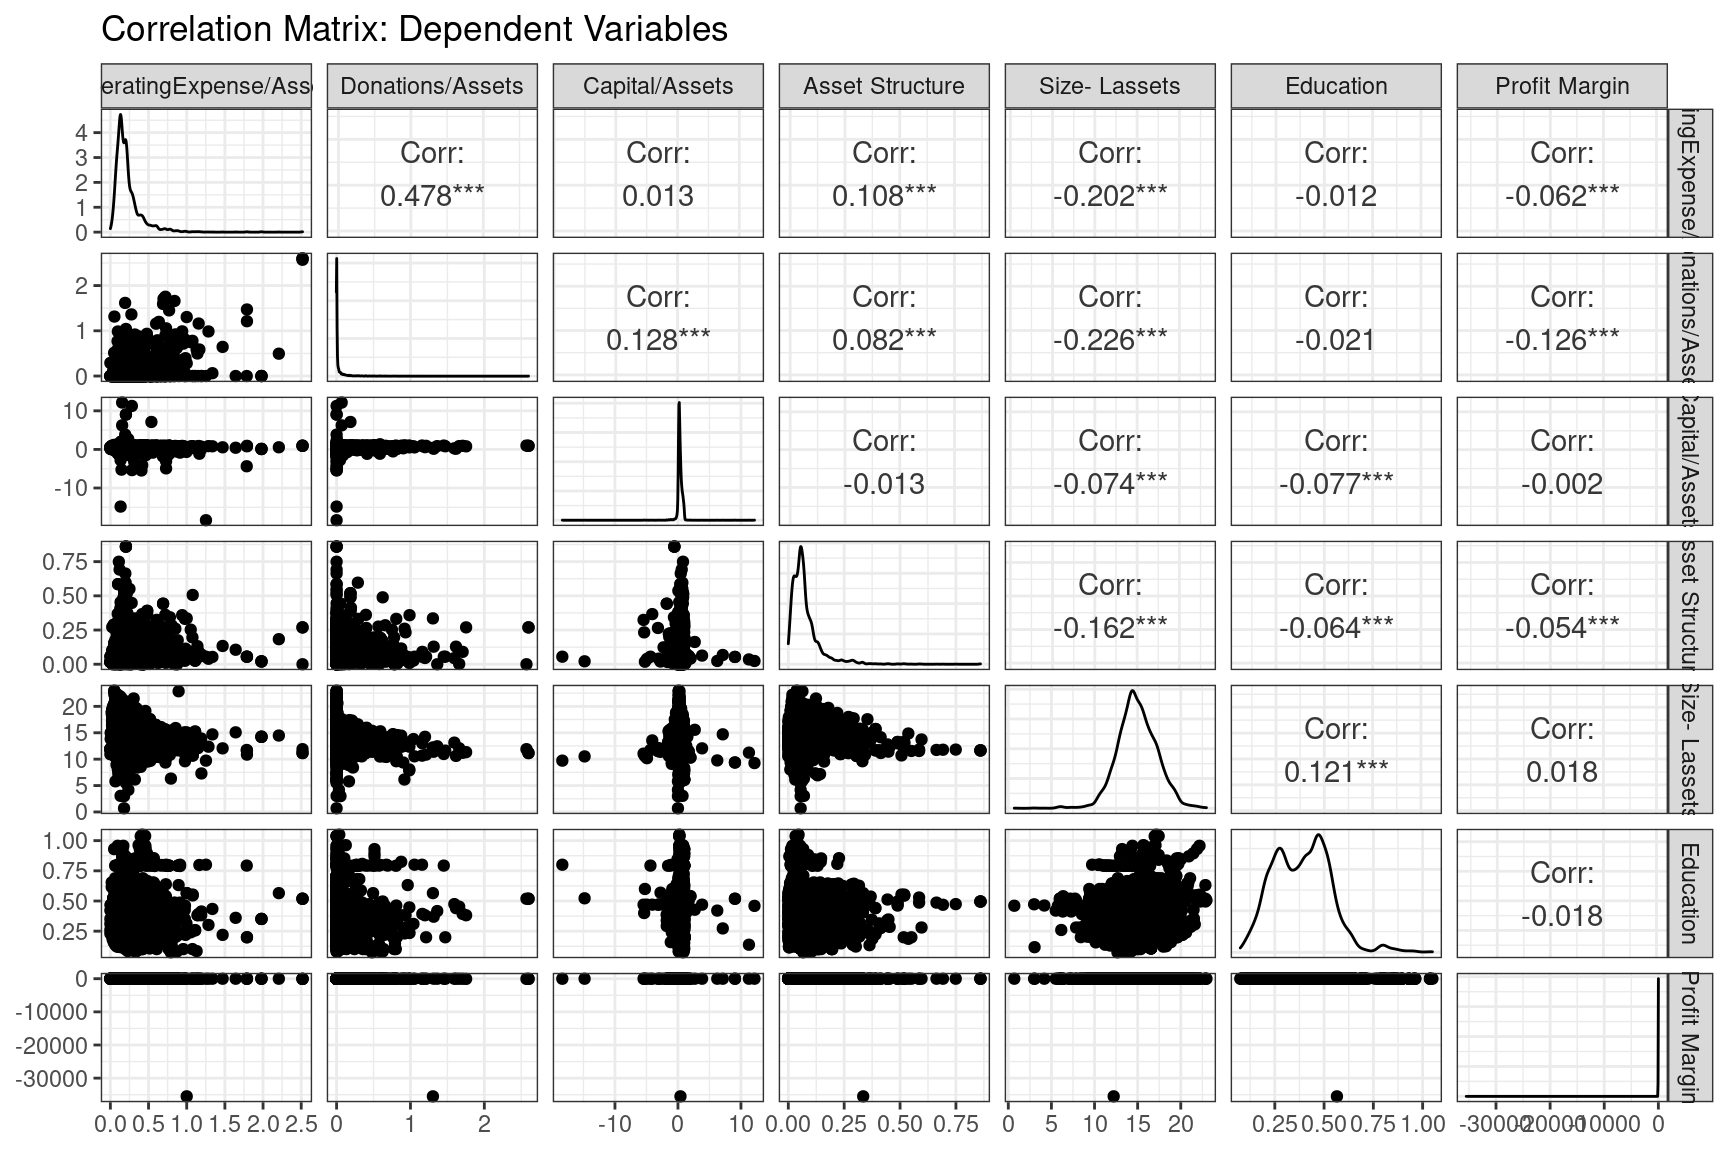
\includegraphics{_main_files/figure-latex/plots2-1.pdf}
\caption{\label{fig:plots2}Correlation Matrix for Independent Variables}
\end{figure}

\end{landscape}

Next, we visualise each of the numeric variables against the current legal forms (status) of MFIs. We use the median of the variables to stand for the variables. Figure 3.2 (Panel A) shows that mature MFIs form the bulk of MFIs in the sample. Among mature MFIs, NGOs and cooperatives are the majority, indicating their relatively longer operational cycle than NBFIs, banks, and rural banks. As expected, NGOs receive the highest share of donations, followed by credit unions and NBFIs, while commercial banks receive the least donations (Figure 3.2- Panel B). The result relating to NGOs is not surprising given they are rooted in the welfare model of microfinance. Most donors are likely to channel their funds to MFIs that place social performance over profits. When commercial capital almost entirely replaces donations, outreach to the poor may likely be affected \autocite{roberts2013profit}, given that managers may emphasise impressing shareholders and debt-holders in line with the agency theory. As noted by \textcite{d2013unsubsidized}, MFIs with little or no subsidies exhibit more significant mission drift. Hence, outreach to the poor would suffer even more where the capital providers do not have a sense of the hybrid nature of microfinance. Therefore, the rise of blended finance where commercial capital funds social causes may partly mitigate this scenario \autocite{attridge2019blended}.

Donations do not prevent NGOs and NBFIs from raising capital as they have the highest capital to assets ratio- which primarily reflects equity injections (Figure 3.2: Panel C). Commercial banks, credit unions and rural banks follow in that order. The observation is surprising given that NGOs and NBFIs still exhibit a high level of social performance even with a relatively high capital to assets feature. Therefore, it could imply that the profit vs social orientation of an MFI could be driven not just by the needs of the providers of funds but also by the internal governance, mission, and strategic direction of an MFI \autocite{campion1999institutional}. In this respect, an MFI's social mission could outweigh the needs of capital providers. Also, the equity capital NGOs may attract may be preferential in terms of expected returns, as with blended finance \autocite{rode2019blended}. In this case, donors could provide dedicated capital that does not pressure management to make high interest or dividends payments, allowing MFIs to remain predominantly on the social mission path \autocite{lopatta2016microfinance}. \footnote{Apart from credit unions/cooperatives and rural banks, we use acronyms for other legal forms of MFIs. NGO stands for non-governmental organisations, while NBFI connotes non-bank financial institutions. The term bank represents microfinance-oriented commercial banks.}

Appendix 10 and 11 show the visualisation for the debt to equity ratio and deposits to assets ratio. While NGOs attract more equity capital, rural banks, commercial banks, and credit unions rely more on debt, especially deposits form of debt, to finance their operations. The analysis shows that while all MFIs are raising capital, the sources are different for commercial MFIs vis-a-vis NGOs. While NGOs are inclined to using more equity, commercial MFIs appear to rely more on debt. Debt capital gives rise to fixed obligations that may exacerbate mission drift, and hence the conversion of NGOs to commercial entities could be harmful to social outreach. However, the relative inability to garner deposits maybe detrimental to NGOs' ability to access cheap, less restrictive capital.

Lastly, for asset structure (tangibility), the ratio of non-current assets to total assets, credit unions lead followed by commercial banks, NGOs, NBFIs, and rural banks. Asset structure captures the extent to which MFIs invest in physical infrastructure relative to the total asset base. Credit unions tend to serve a narrow geographic region and traditionally put up brick and mortar branches to serve their customers \autocite{mckillop2011credit}. Like credit unions, commercial banks tended to have more branches, having taken root before the advent of fintech, reducing the need for physical branches. NGOs, NBFIs, and rural banks have the lowest rates of asset tangibility, especially those of more recent origins, and using rural agents to meet customers rather than set up an expansive network of branches \autocite{kent2013bankers}.

Figure 3.3 (Panel A) shows that NGOs exhibit the highest median operating expense to assets ratio followed by NBFIs while credit unions trail. As we see later in the analysis, operating expenses positively relate to the depth of outreach- per cent of female borrowers and breadth of outreach in terms of gross loans to assets. Therefore, NGOs will do better in social outreach as they incur more costs to reach out to the financially excluded. Indeed, literature shows that outreach to the poor is expensive partly due to the dis-economies of scale in serving the poor, financially excluded clients \autocite{mia2017mission}. One of the efficiency enhancement opportunities from the transformation of MFIs to the for-profit approach to microfinance services delivery is that managers could trim operating expenses to increase profits hurting financial inclusion.

Turning to profitability in Figure 3.3 (Panel B), we find that rural and commercial banks post the highest median profits, while NBFIs and NGOs trail (Figure 3.3- Panel B). This result probably partially illustrates the emphasis on social performance over financial performance by the management. NGOs and NBFIs are more likely to favour the social goal. When we take this result together with the observation that NGOs tend to have more operating expenses, we conclude that the desire by managers of commercial banks and other for-profit MFIs to mitigate agency conflicts leads to less operating expenses, more profitability and, hence, lower outreach to the financially excluded \autocite{jensen1976theory}.

Overall, the pattern indicates that while NGOs spend the most in operating expenses to reach the financially excluded, these efforts come at the cost of profitability. In contrast, profit-oriented MFIs are keen to manage expenses that improve profitability, presumably at the expense of outreach to the financially excluded. It is worth noting that NGOs have a relatively low asset base and hold relatively fewer non-current assets to total assets. The observation could mean that NGOs do not invest heavily in brick and mortar branches or serve a relatively limited geographic range. Finally, NGOs have the highest capital (equity) to asset ratio despite the push towards commercial capital. Much could be from investors, who put forth dedicated equity capital because they are keen on social performance and not profits \autocite{mia2017mission}.

We now turn to Figure 3.4. The first graph (Figure 3.4- Panel A) shows that commercial banks have the most prominent asset size (total assets), while NGOs and cooperatives have the smallest in that order. Banks tend to have a much broader geographic presence and hence attract more clients, which means more assets accumulation. Again, capital adequacy requirements by central banks have implications on the assets that banks hold. Furthermore, commercial banks are generally dominant in many developing countries meaning that they have a long operating history which implies a bigger size \autocite{levine2002bank}. Figure 3.4 panel B shows that NGOs and NBFIs serve proportionately more women borrowers, indicating their outreach depth. Given that much of the donor funds accrues to NGOs, the conversion to the for-profit model would be detrimental to financial inclusion if coupled with a reduction in donor funding.

Commercial banks and credit unions have the highest average loan balance per borrower (depth of outreach), while NBFIs and NGOs come last in that order (Figure 3.4- Panel C). As an indicator of outreach to the poor, the average loan balance per borrower is better when lower, indicating that more impoverished people get access to financial services. Again, it appears that profit-orientation by commercial banks may cause MFIs to reach less financially excluded people in favour of making profits. For credit unions, the observation could arise due to the limited geographic range of operations where they serve people with a common interest like the type of occupation, meaning that their members may not be suffering from financial exclusion in the first place \autocite{armendariz2013subsidy}.

NGOs have the highest median gross loans to total assets ratio, surprising given their relatively smaller size. On the other hand, banks and rural banks, respectively, have the lowest gross loans to assets, meaning they are less efficient in converting their assets into credit (Figure 3.4- Panel D). Again, it shows, at least in the case of Africa, that the breadth and depth of financial outreach are not always mutually exclusive. In this case, NGOs can reach the most impoverished borrowers, going by the per cent of female borrowers and average loan balance per borrower, while at the same time seemingly reaching a broad customer base as indicated by the gross loans to assets. So far, the bulk of MFIs population leans towards the welfare orientation where profitability overtly seems incompatible with outreach to the financially excluded \autocite{lopatta2016microfinance}.

\newpage
\begin{landscape}

\begin{figure}
\centering
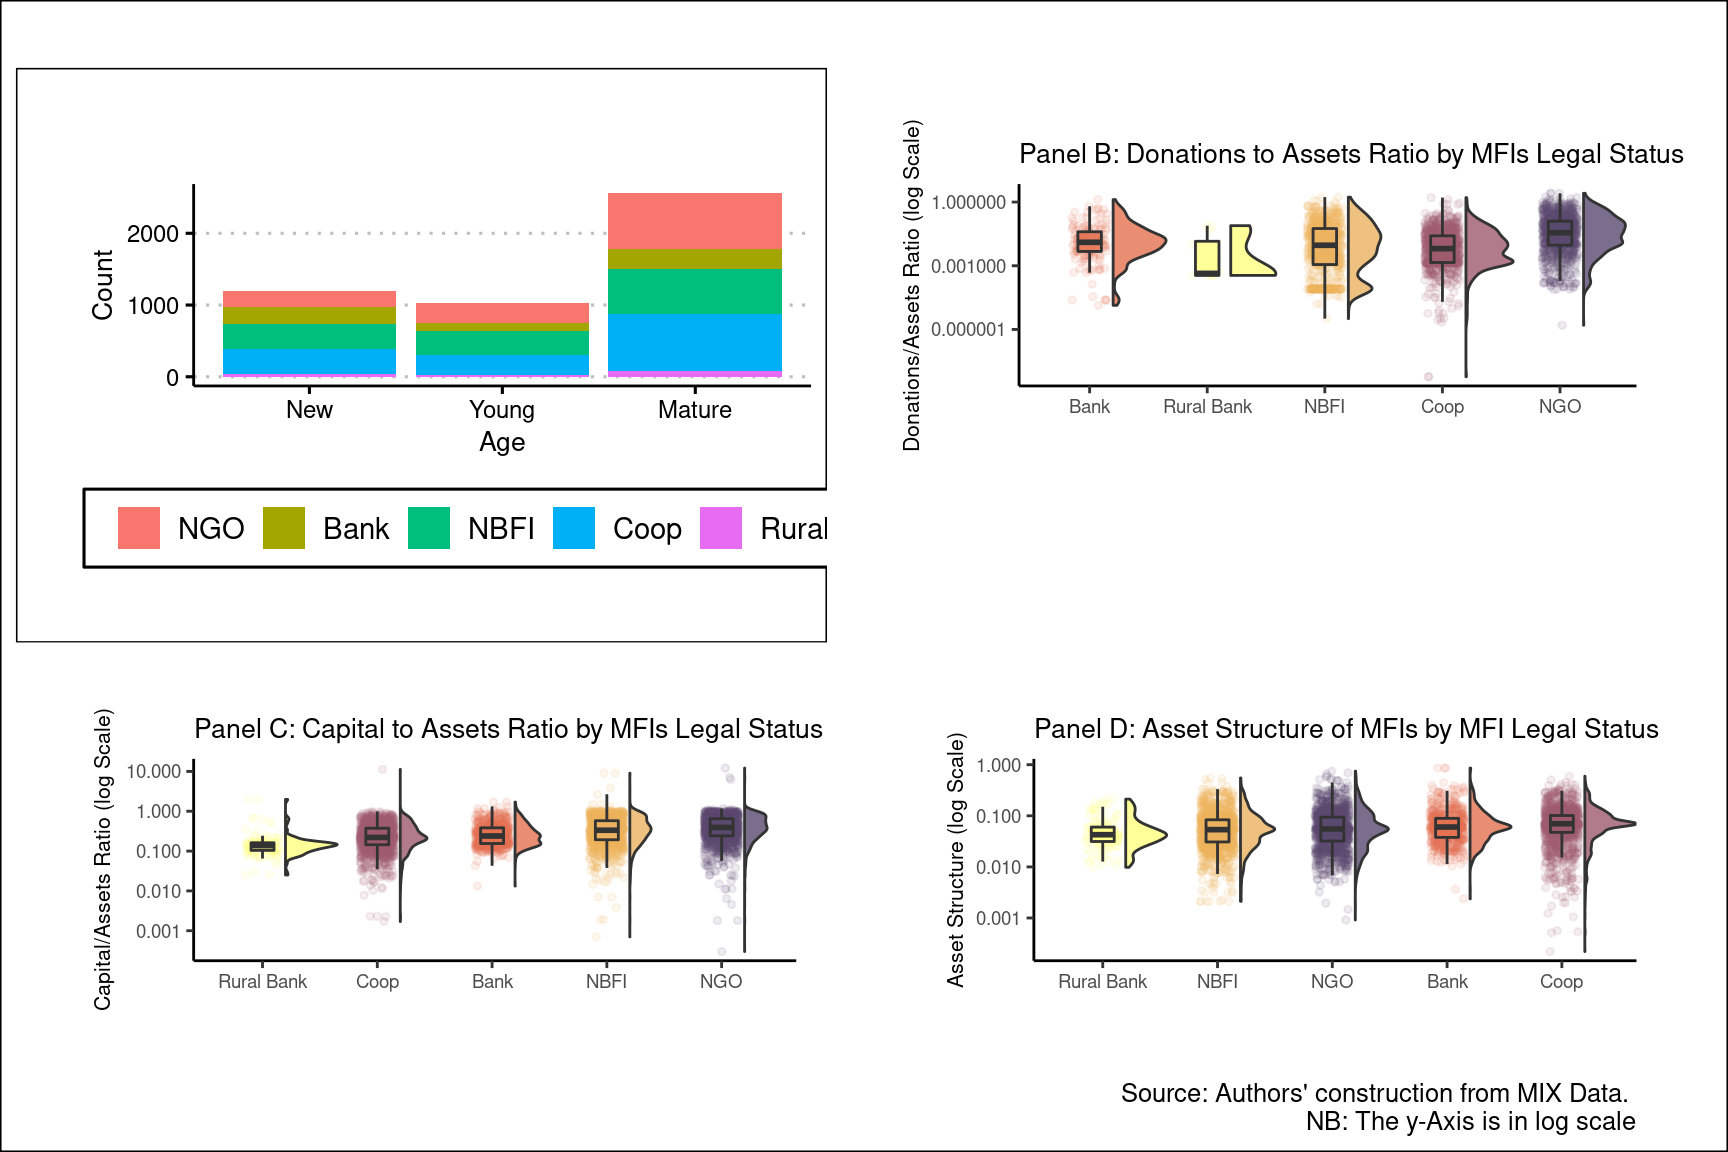
\includegraphics{_main_files/figure-latex/unnamed-chunk-62-1.pdf}
\caption{\label{fig:unnamed-chunk-62}Operating Expense, Donations, Capital and Asset Structure of MFIs by Legal Status}
\end{figure}

\newpage

\begin{figure}
\centering
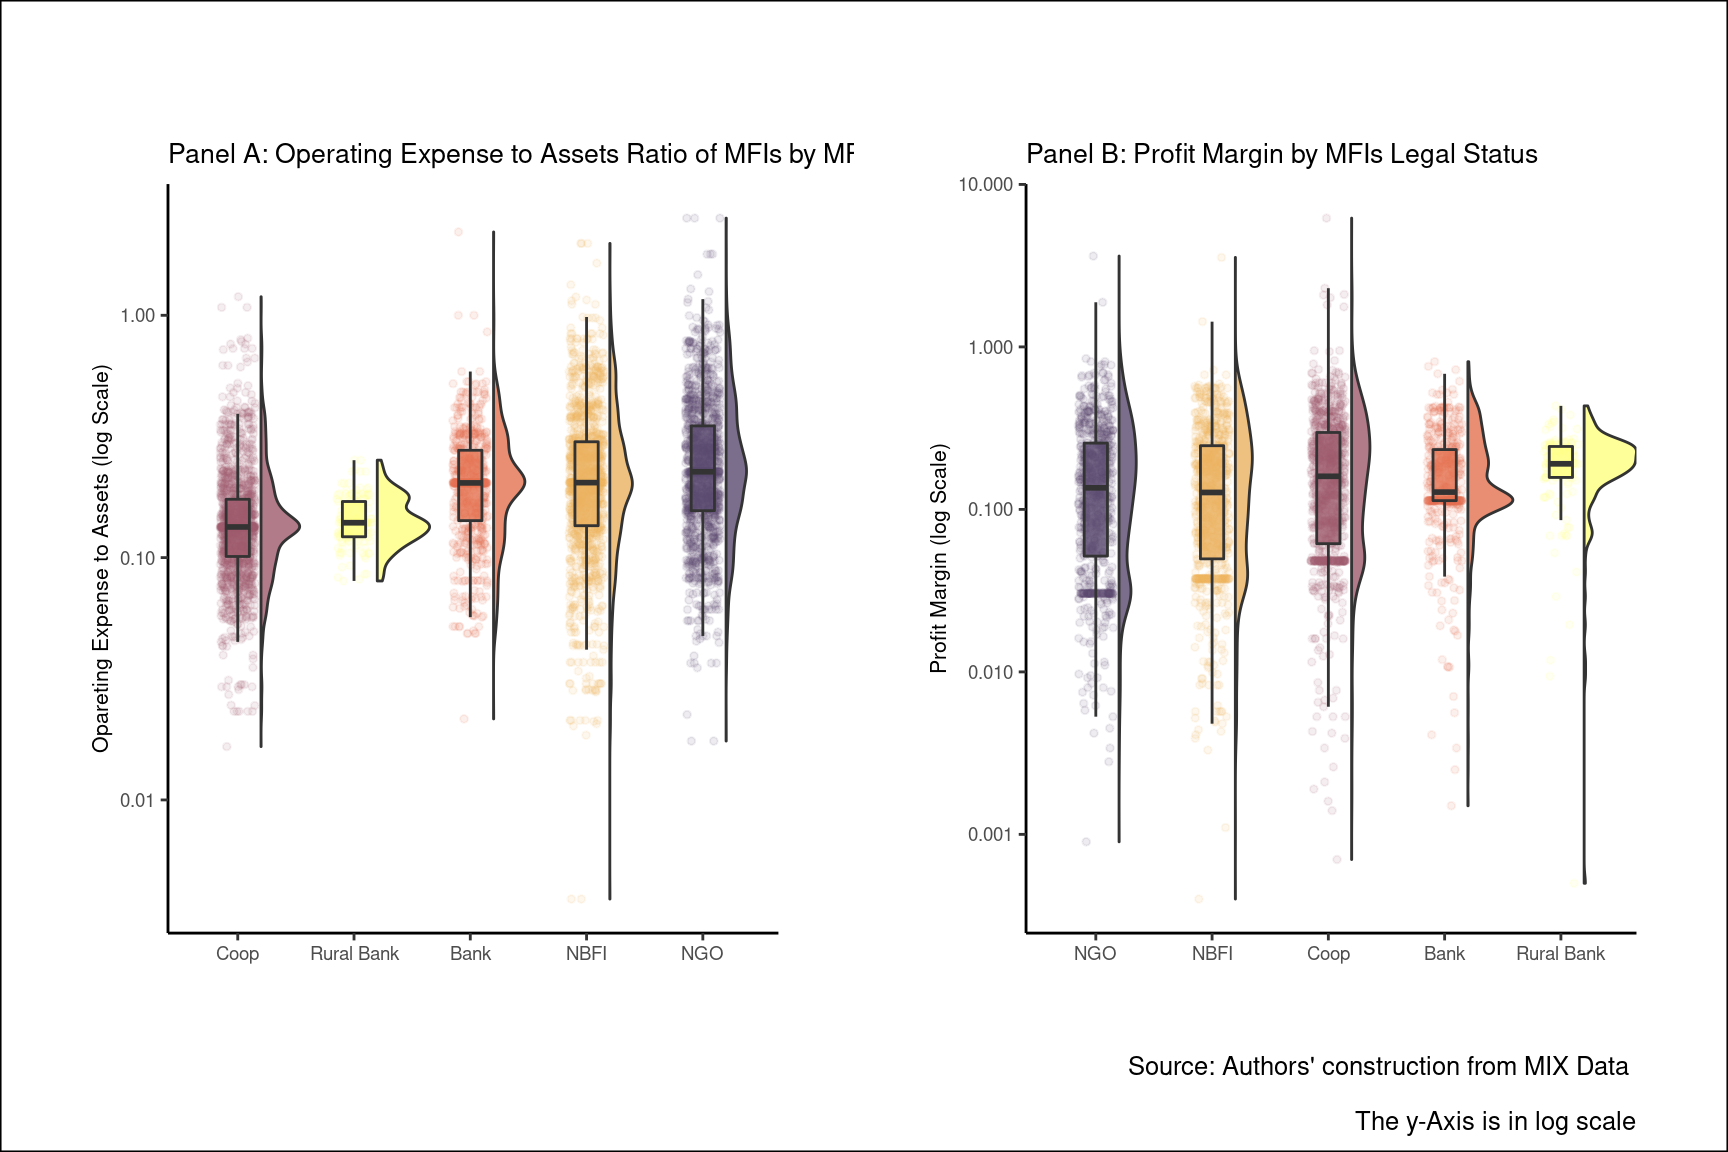
\includegraphics{_main_files/figure-latex/unnamed-chunk-63-1.pdf}
\caption{\label{fig:unnamed-chunk-63}Asset Structure, Profit Margin, Donations, Capital to Assets Ratio by Current Legal Status}
\end{figure}

\end{landscape}

\newpage
\begin{landscape}

\begin{figure}
\centering
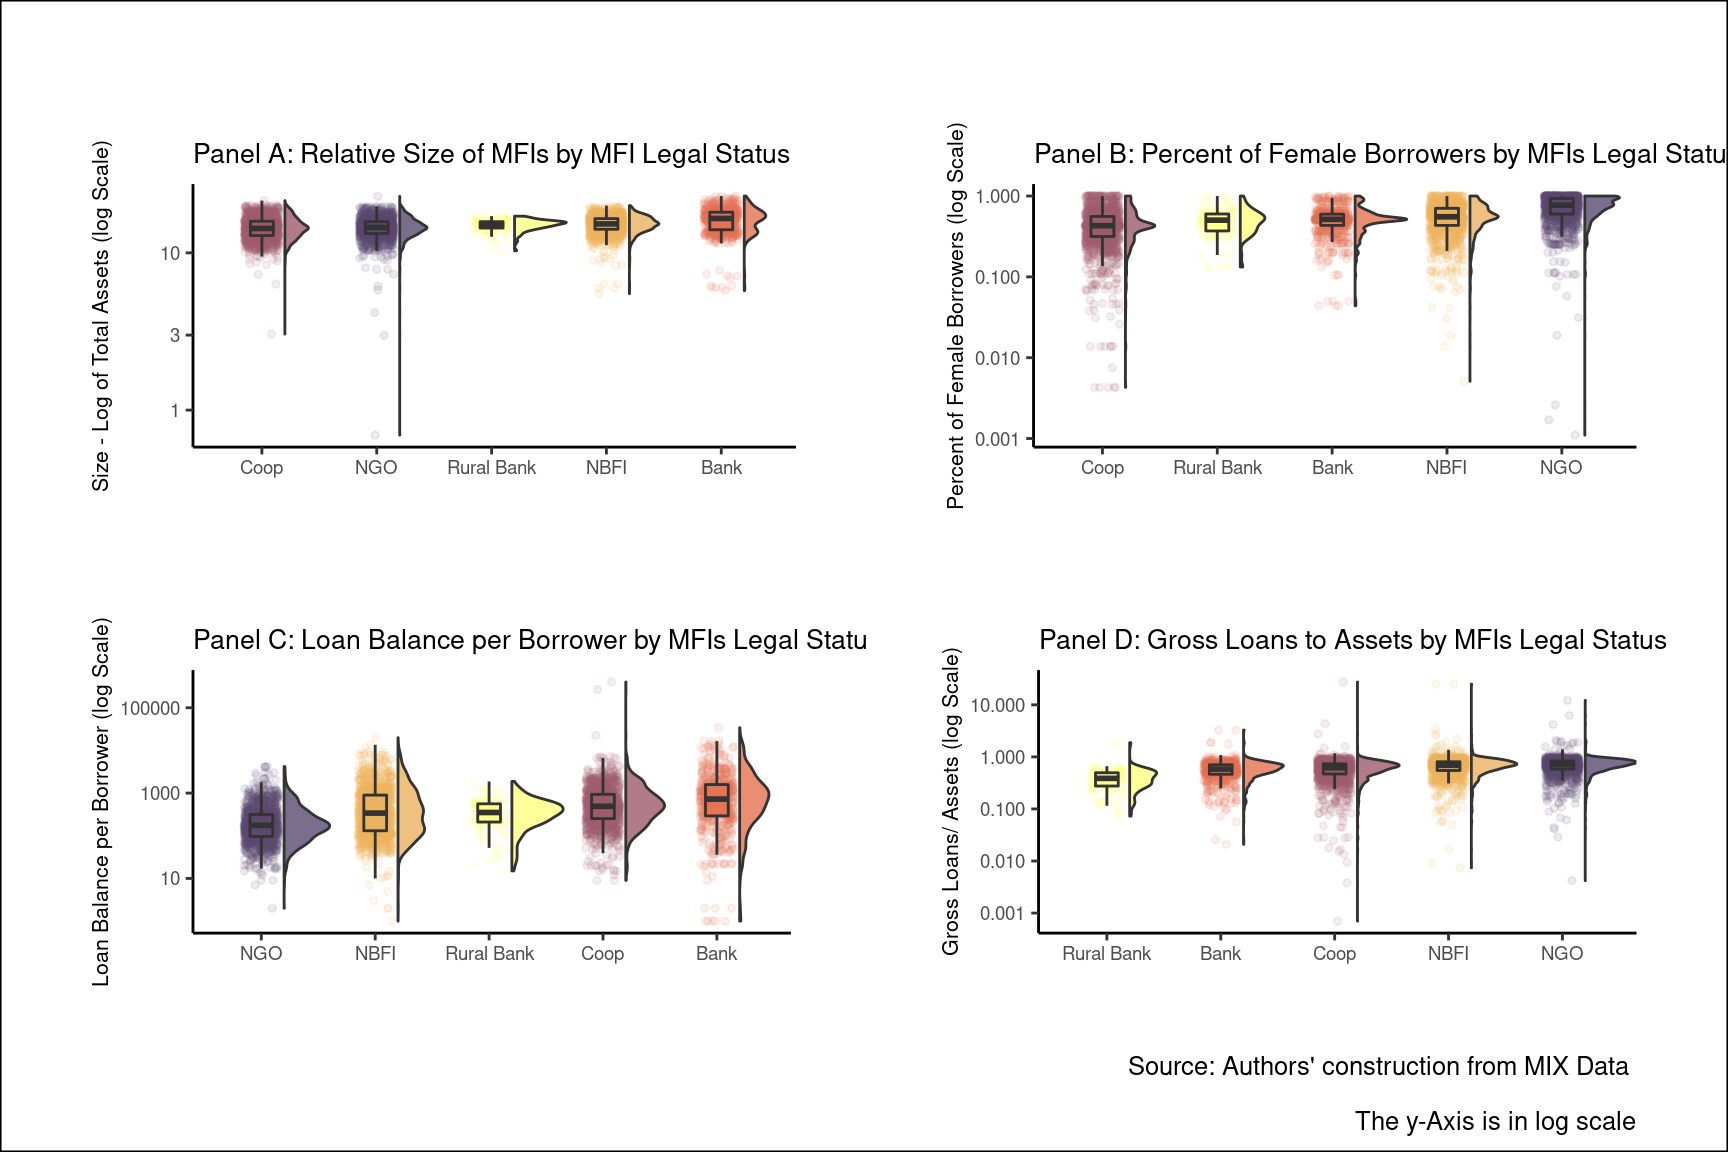
\includegraphics{_main_files/figure-latex/unnamed-chunk-64-1.pdf}
\caption{\label{fig:unnamed-chunk-64}Size, Profit Margin, Average Loan Balance per Borrower and Gross of MFIs by Legal Status}
\end{figure}

\end{landscape}
\newpage

\hypertarget{trends-in-dependent-and-independent-variables}{%
\subsubsection{Trends in Dependent and Independent Variables}\label{trends-in-dependent-and-independent-variables}}

Figure 3.4 below maps the trends, over time, for donations, capital, profits and operating expense to assets ratio, respectively. Figure 3.5 (\emph{Panel A}) shows that the median donations to assets ratio have been downward for 1999-2019. The observation confirms the neo-liberal shift in the MFI paradigm where donors expect MFIs to be more financially self-sustainable. The trend is expected in light of the abundance of literature on the conversion of MFIs from NGOs and subsequent drop in donor funding \autocite{d2017ngos}. As donations dry up, we expect the debt and equity capital components to fill the void.

Surprisingly, the capital to assets ratio, which captures the extent of the equity capital injection, is also on a downward trend despite the drive towards the commercialization of MFIs (\emph{Figure 3.5, Panel B}). The observation could be due to a rise in the total asset base of MFIs, as they scale up, with equity capital being a relatively smaller external capital component than debt. \emph{Appendix 8} shows a steady increase in the debt/equity ratio, which means that most MFIs, like commercial banks, use debt (including deposits) to finance their operations. In this respect, debt gives rise to fixed obligations which could hurt profitability during economic downturns.

MFI profitability in Figure 3.5 (\emph{Panel C}) shows that the median profitability for MFIs is meager and almost invariant over time, except *for a significant dip in mean profitability around 2008-2009 during the global financial crisis period. The result is consistent with the empirical regularity that shows microfinance as a low margin business, largely reflecting the primacy of social mission in microfinance \autocite{hartarska2012governance}. An important observation is that there are no distinctive profitability changes even as more MFIs adopt the commercial model. This observation means that either the commercialization was not very successful in generating profits or that the extent to which MFIs were able to make profits post-transformation is particularly peculiar to each MFI or to each of the legal forms of MFIs.

Lastly, for Figure 3.5 (\emph{Panel D}), the operating expenses to assets ratio remains approximately constant except for a dip in the 1999-2001 period. As the regressions show in a later section, the operating expense to assets ratio relates positively to outreach depth and breadth. In this case, the drop in the ratio between 1999 and 2001 could have worsened financial inclusion outcomes. However, the operating expenses to assets ratio have levelled off; thus, it could be indicating a sustained commitment to outreach even in the face of the desire to make profits.

Next, we turn to Figure 3.6, which shows a rise in MFI size, average loan balance per borrower, and gross loans to total assets, while the per cent of female borrowers is on a downward trend. The rise in the average loan's balance per borrower and the accompanying drop in the proportion of female borrowers indicates a consistent decline in the outreach of MFIs to the financially excluded, as MFIs rely less on donations and more on commercial capital. It further shows the effects of the neo-liberal, for-profit paradigm, which may be hurting the social performance of MFIs, precisely the depth of outreach. However, it appears the breadth of outreach is getting better with time as MFIs give more loans. Taken together, it implies that MFIs provide larger loans to less financially excluded people in a bid to make ample financial return to allow for financial sustainability and payment of dividends and interest to investors.

Appendices 12-14 show the breakdown, by legal forms of MFIs, of the trends for per cent of female borrowers, average loan balance per borrower and gross loans to assets. The movement is generally downwards for women borrowers except under the commercial banking legal forms, which have low outreach to women, but that is relatively constant after the initial spike in the early 2000s. The trends indicate a weakening depth of outreach. For average loan balance per borrower, NGOs and rural banks remain relatively constant. At the same time, other legal forms have rising average loan size trends, which indicates worsening outreach by banks, credit unions, and NBFIs. Lastly, gross loans are rising except for rural banks, showing a better breadth of outreach over time.

\begin{landscape}
\newpage

\hypertarget{descriptive-statistics-trends-over-2000-2020}{%
\subsection{Descriptive Statistics: Trends Over 2000-2020}\label{descriptive-statistics-trends-over-2000-2020}}

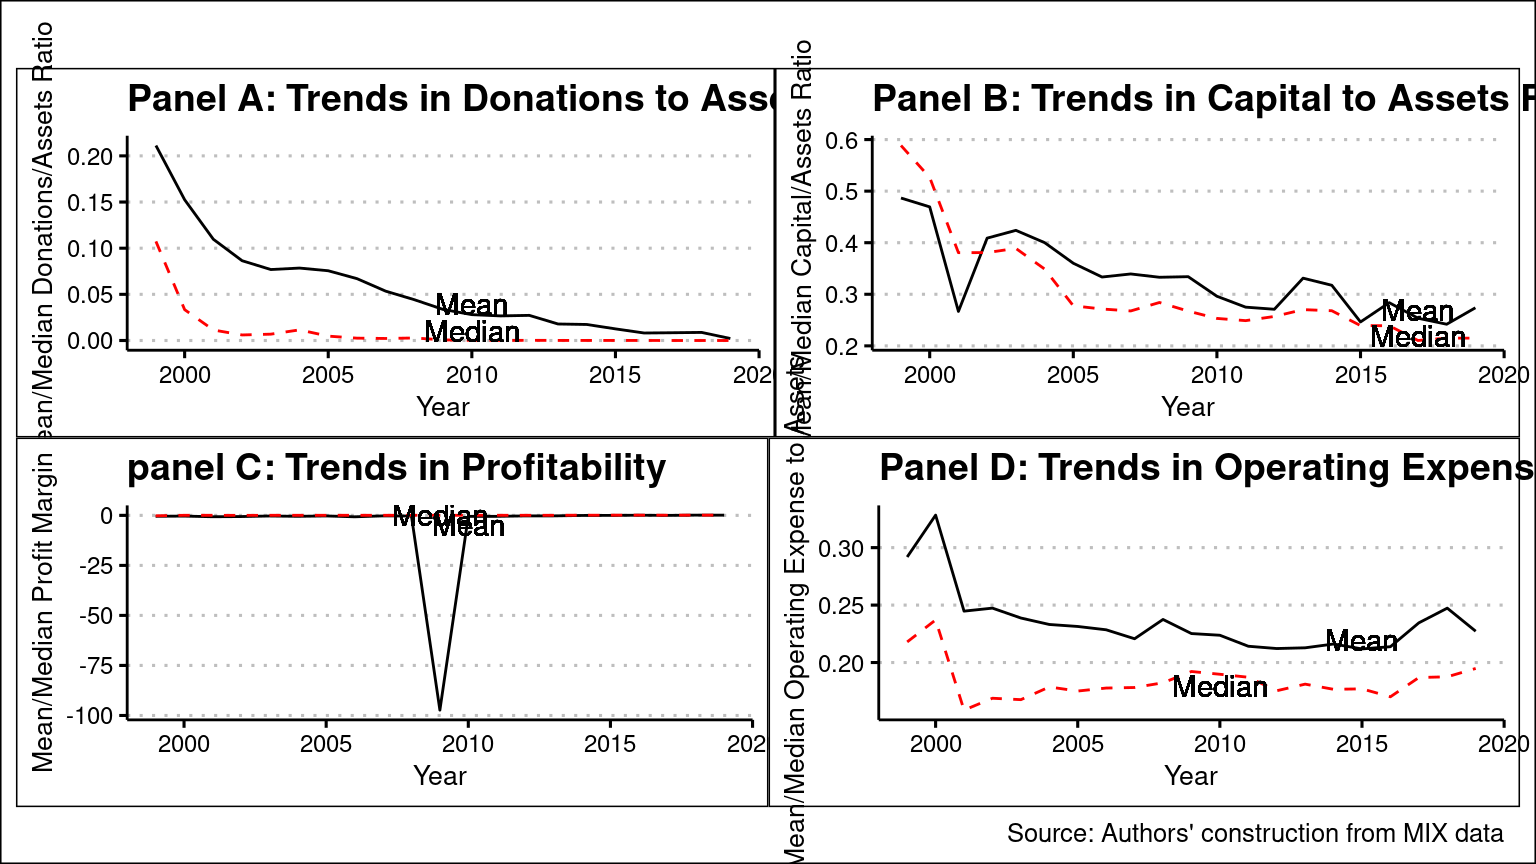
\includegraphics{_main_files/figure-latex/unnamed-chunk-66-1.pdf}

\newpage

\begin{figure}
\centering
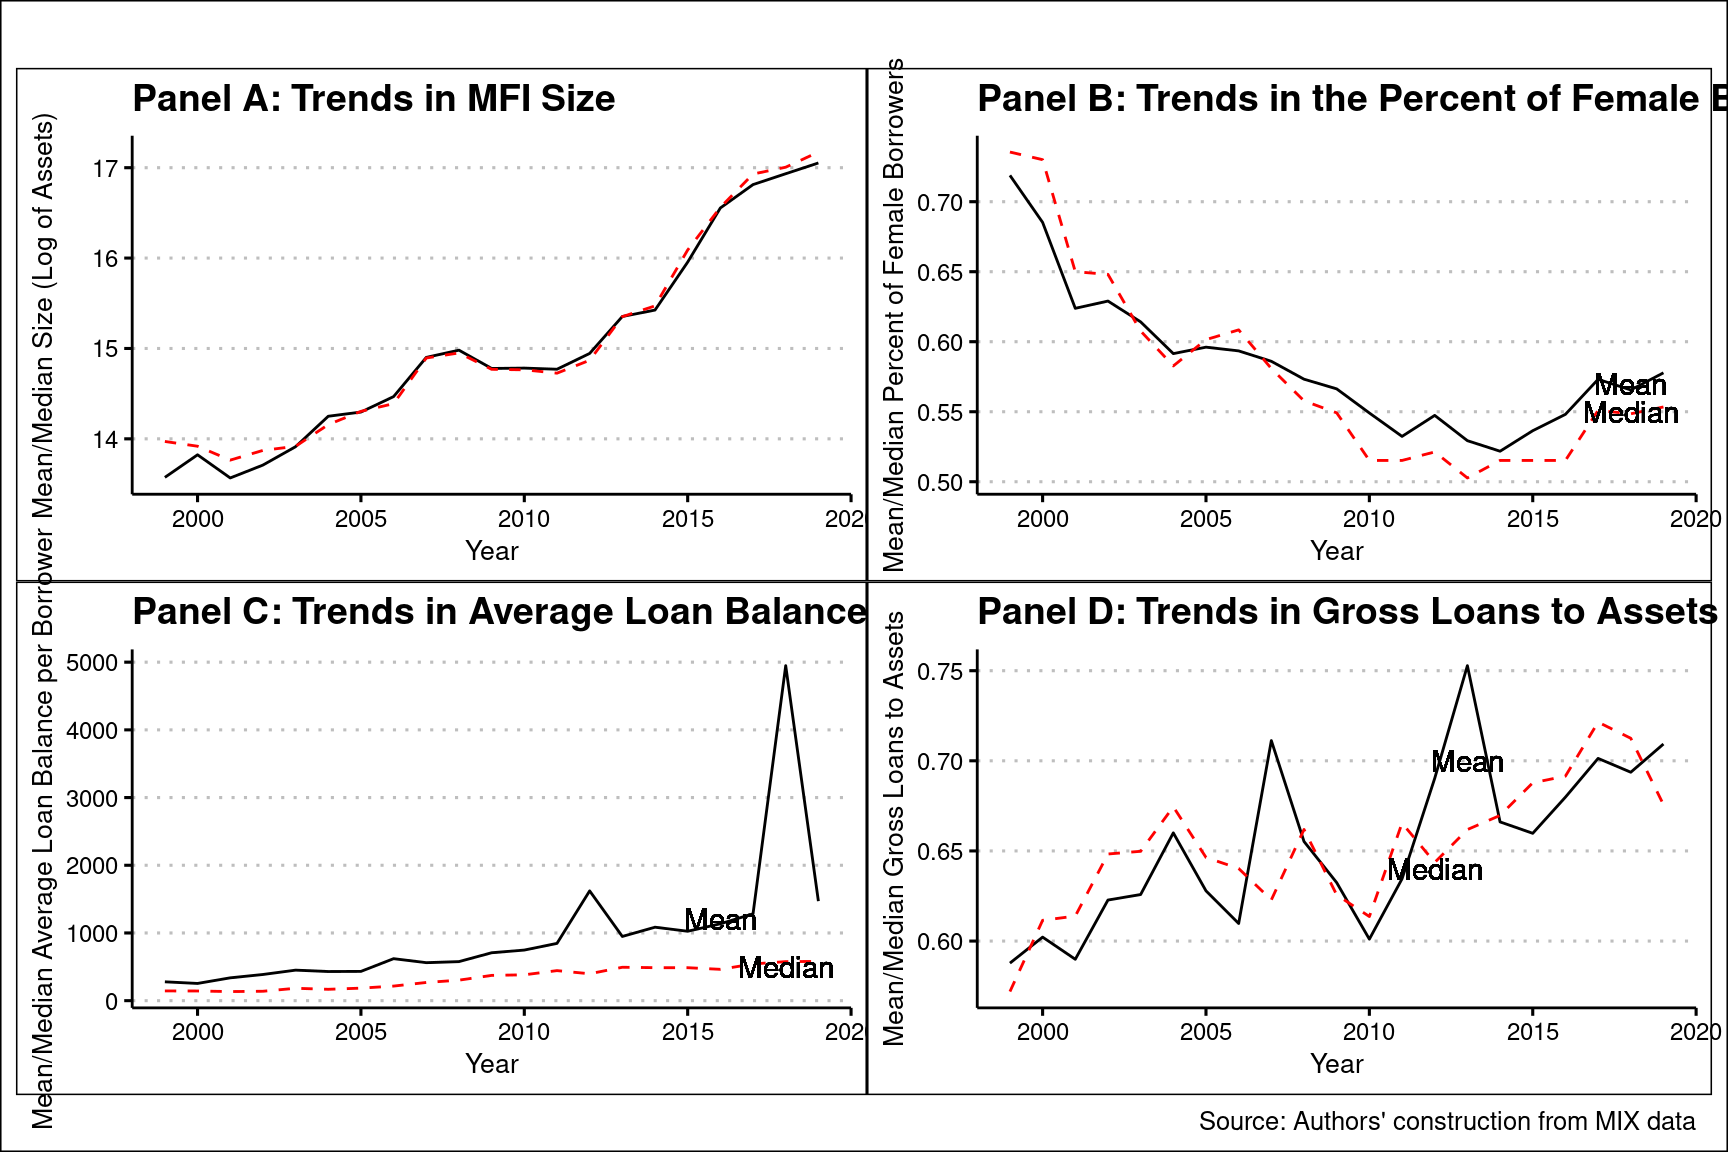
\includegraphics{_main_files/figure-latex/unnamed-chunk-67-1.pdf}
\caption{\label{fig:unnamed-chunk-67}Trends in MFI Size, Female Borrowers, Average Loan Balances, and Gross Loans}
\end{figure}

\end{landscape}

\hypertarget{summary-statistics-1}{%
\subsection{Summary Statistics}\label{summary-statistics-1}}

Tables 3.2 and 3.3 show the summary statistics of the variables applied in the regression analysis later on. The summary indicates that there is not a wide variation in the composition of the legal forms of MFIs, with banks (619) and rural banks (138) having the least number of entities in the sample dataset. Turning to age, mature MFIs dominate in the sample dataset, followed by new MFIs (0-4 years) and young MFIs (4-8 years). Table 3.3 shows a summary of the three dependent variables. We have visualized and discussed the breakdown of these variables by MFI legal status in Figure 3.4.

\begin{table}

\caption{\label{tab:unnamed-chunk-68}Summary Statistics for Categorical Independent Variables}
\centering
\fontsize{9}{11}\selectfont
\begin{tabu} to \linewidth {>{\raggedright}X>{\raggedright}X}
\toprule
Variable & Counts\\
\midrule
Current Legal Status & Credit Unions: 1427, NBFI: 1315, NGO: 1250, Bank: 619\\
Age & Mature: 2558, New: 1200, Young: 1024\\
\bottomrule
\multicolumn{2}{l}{\rule{0pt}{1em}Source: Authors' construction from the MIX data}\\
\multicolumn{2}{l}{\rule{0pt}{1em}\textit{Note: }}\\
\multicolumn{2}{l}{\rule{0pt}{1em}\textsuperscript{1} Legal status include NGO, Non-Bank Financial Institutions (NBFIs), Credit Unions, and Banks}\\
\multicolumn{2}{l}{\rule{0pt}{1em}\textsuperscript{2} Age has mature MFIs older than 8 years, young ones (4 - 8 years), and new ones that are 4 years or less}\\
\end{tabu}
\end{table}

\begin{table}

\caption{\label{tab:unnamed-chunk-69}Summary Statistics for Numeric Dependent Variables}
\centering
\fontsize{9}{11}\selectfont
\begin{tabular}[t]{lrrrrr}
\toprule
Variable & Mean & SD & Q1 & Median & Q3\\
\midrule
percent\_of\_female\_borrowers & 0.569 & 0.237 & 0.421 & 0.550 & 0.748\\
average\_loan\_balance\_per\_borrower & 895.001 & 7332.114 & 142.000 & 335.000 & 776.500\\
gross\_loan\_portfolio\_to\_total\_assets & 0.655 & 0.712 & 0.504 & 0.654 & 0.777\\
\bottomrule
\multicolumn{6}{l}{\rule{0pt}{1em}Source: Authors' construction from the MIX data}\\
\multicolumn{6}{l}{\rule{0pt}{1em}\textit{Note: }}\\
\multicolumn{6}{l}{\rule{0pt}{1em}\textsuperscript{1} The summary statistics are disaggregated by MFI legal status}\\
\end{tabular}
\end{table}

\begin{table}

\caption{\label{tab:unnamed-chunk-70}Summary Statistics for Continous Independent Variables}
\centering
\fontsize{10}{12}\selectfont
\begin{tabular}[t]{lrrrrrrr}
\toprule
Variable & Mean & SD & Min & Q1 & Median & Q3 & Max\\
\midrule
operating\_expense\_assets & 0.227 & 0.185 & 0.000 & 0.124 & 0.181 & 0.269 & 2.52\\
donations\_assets\_ratio & 0.043 & 0.147 & -0.003 & 0.000 & 0.001 & 0.019 & 2.60\\
capital\_asset\_ratio & 0.321 & 0.602 & -18.353 & 0.153 & 0.273 & 0.478 & 12.15\\
asset\_structure & 0.076 & 0.069 & 0.000 & 0.035 & 0.060 & 0.092 & 0.86\\
assets & 14.946 & 2.262 & 0.693 & 13.540 & 14.858 & 16.416 & 22.98\\
\addlinespace
education & 0.387 & 0.144 & 0.075 & 0.273 & 0.386 & 0.487 & 1.05\\
profit\_margin & -7.739 & 513.299 & -35495.625 & -0.181 & 0.048 & 0.189 & 6.20\\
\bottomrule
\multicolumn{8}{l}{\rule{0pt}{1em}Source: Authors' construction from the MIX data}\\
\multicolumn{8}{l}{\rule{0pt}{1em}\textit{Note: }}\\
\multicolumn{8}{l}{\rule{0pt}{1em}\textsuperscript{1} The summary statistics are disaggregated by MFI legal status}\\
\end{tabular}
\end{table}

\newpage

\hypertarget{regression-analysis}{%
\subsection{Regression Analysis}\label{regression-analysis}}

This section describes the results of the deeper data analysis, that is, regression models in Table 3.5 and 3.6, and Appendix 1 taken alongside the results of the exploratory data analysis. Table 3.5 shows the output for the fixed effects model (see results of the Hausmann test in Appendix 2) \footnote{The link to the WDI database is \url{https://databank.worldbank.org/source/world-development-indicators}.}. Table 3.6 presents the results of the random effects and the pooled OLS models. We describe the impact of transformation on each dependent variable: the MFI outreach proxies of per cent of women borrowers, average loan balance per borrower, and gross loans to assets. We are working with an unbalanced panel dataset; we run three regressions for each outcome variable. First, we run the regression using the entire dataset, then rerun the regression using data for MFIs with at least three years (panels) of data. Lastly, we run another regression for MFIs with at least five years of data \footnote{The link to the GFDD is \url{https://www.worldbank.org/en/publication/gfdr/data/global-financial-development-database}.}. Table 3.5 shows the results of the fixed-effects model, while Table 3.6 presents the random effects and pooled OLS models. The discussion that follows mainly draws from the fixed and random-effects models.

\hypertarget{percent-of-women-borrowers}{%
\subsubsection{Percent of Women Borrowers}\label{percent-of-women-borrowers}}

The legal status of an MFI is a significant driver of outreach to women, with NGOs faring better (see Table 3.6). Note that NGOs are the base outcome in current legal status, while banks, NBFIs, cooperatives/credit unions, and rural banks are the alternative outcomes. The basis for picking NGOs as the base outcome stems from the trend of NGOs converting to the commercial model, the core of this article. Other positive outreach drivers include education, operating expenses to assets ratio, profit margin, and capital-to-assets ratio. North Africa fares worse in MFI outreach than Sub-Sahara Africa despite being represented entirely by NGOs in the sample, showing the importance of considering regional disparities. Table 3.6 of the random effects and pooled OLS model shows that NGOs outperform other legal forms of MFIs in reaching out to women. The result implies that the transformation of MFIs can negatively impact financial inclusion efforts as commercial MFIs are less keen to reach the financially excluded, which contradicts some previous research \autocite{ledgerwood1998microfinance,ledgerwood2006transforming,hartarska2012governance,bos2015practice}. Again, the results highlight the potential regional disparities even within Africa, which may question the inferences made using global datasets.

The results gain more credence when examining the operating expenses to assets ratio (Table 3.5 and 6). There is a positive and significant relationship between operating expense to assets ratio on the one hand and per cent of women borrowers on the other. It means that an MFI has to spend more to reach financially excluded clients, which means lesser profits at a given level of revenue. As expected, the conversion of MFIs from NGOs to the commercial model could reduce operating expenses in the quest for profits in line with the profit incentive arising from the agency theory \autocite{eisenhardt1989agency}. Hence, it arguably follows that pursuit of profit is bad for financial inclusion by causing mission drift in line with prior research \autocite{wagenaar2012institutional,roberts2013profit,lopatta2016microfinance,mia2017mission}. Except in the unlikely scenario where MFIs generate profits by raising revenue without lowering costs, Africa's MFIs and regulators should rethink the case for the transformation of MFIs into the commercial model \autocite{sun2021globalization}.

Indeed, profitability has a positive relationship, albeit insignificant on women borrowers' per cent (see Table 3.5 and 3.6). With this hindsight, it would appear like the viable explanation for the profitability-operating expense-financial inclusion issue is that for commercial MFIs, it is to reduce operating expenses in the short run if that translates into higher profits. Higher profitability allows the MFIs to reach more financially excluded clients while cross-subsidising them in the medium to long term. \textcite{d2017ngos} note that for transformed MFIs, profits tend to drop in the short term but not necessarily in the long term. The drop in profitability is driven by transformed MFIs charging lower interest rates, a contentious issue in micro-finance. Therefore, it would be worth examining the dynamics between profitability, operating expense, and financial inclusion for MFIs over a more extended period.

The significant control variables are education (Table 3.5 and 3.6) and region (table 3.6). Education varies positively with outreach to women, as does region. MFIs in Northern Africa have lower outreach to women than an otherwise similar MFI in Sub-Saharan Africa. These results could be due to religious beliefs or practices that discount financial inclusion outcomes for women or a conscious shift to the Islamic model against charging interest on capital \autocite{hassan2018religious}. This observation is despite North Africa being represented only by NGOs in the sample. Our previous findings show that NGOs have higher outreach to women than other legal forms of MFIs. The implication is that cultural and religious inclinations play a more significant role in driving financial inclusion than the operating model of MFIs in North Africa. Education also appears to play a key role in financial inclusion by empowering women to join the formal labour market and equipping women with financial literacy that allows for better financial decision making \autocite{zins2016determinants,chikalipah2017determines}.

These observed relationships hold even when we winsorise the data (see \emph{Appendix 1}). The only exception is the capital to assets ratio and profit margin, which have a significant positive relationship with outreach to women. These results suggest that larger firms are more likely to experience mission drift after conversion. However, even after winsorising the data, NGOs still do better at financing women in line with research from the welfare approach to microfinance \autocite{kodongo2013individual}. To sum this up, MFIs would best achieve the quest to improve outreach to women by targeting NGOs with capital funding, especially with the rise of blended finance, commercial capital for social projects, ceteris paribus. Some other variables in the model are not significant but are worth mentioning. For instance, older firms have lower levels of outreach to women, which could imply that firms lose focus on financial inclusion as they mature and get financially independent. Next, we examine the effects on another measure of the depth of outreach, the average loan balance per borrower.

\hypertarget{average-loan-balance-per-borrower}{%
\subsubsection{Average Loan Balance per Borrower}\label{average-loan-balance-per-borrower}}

Like the per cent of female borrowers, the average loan balance per borrower captures how deep an MFI goes to reach the financially excluded, who typically would demand smaller denominations of loans. Thus, the smaller the average loan balance, the deeper the outreach. The major criticism of the average loan balance per borrower as an indicator of financial inclusion is that a larger average loan balance could result from progressive lending or arise as clients become better off \autocite{abeysekera2014sustainability}. Again, researchers could be wrongly proclaiming mission drift for MFIs operating in countries that have relatively fewer indigent clients \autocite{armendariz2013subsidy}. Notably, the presence of a few vast loans granted to some clients could tilt the average loan balance upwards \autocite{market2014global}. Despite these shortcomings, the metric of average loan size is helpful because it is easily quantifiable, and the relevant data inputs are readily available. \footnote{The link to the GFDD is \url{https://www.worldbank.org/en/publication/gfdr/data/global-financial-development-database}.}.

The key observation in the description of this result is that NGOs consistently offer smaller average loan sizes than other legal forms of MFIs. However, the effect is only significant for credit unions/ cooperatives. Consistent with the outreach to women, the observation would suggest that NGOs reach the financially excluded better than do commercial MFIs. It would then imply that the conversion of MFIs from NGOs to other legal forms is harmful to financial inclusion, as the welfare school argues. In fact, \textcite{d2017ngos} and \textcite{mia2017mission}, using a global dataset of MFIs, find that average loan balances go up after transformation, which is consistent with our finding. Accordingly, \textcite{peck2001commercialization} argue that commercial logic has, over time, displaced the welfare approach in addressing financial exclusion.

Furthermore, older MFIs have a lower average loan balance per borrower relative to newer ones. The relationship could hold as older firms tend to reach out to more financially excluded clients given their stable financial base, operational experience, and linkage to donors who emphasise social performance \autocite{bos2015practice}. However, the larger the MFI's asset base, the higher the average loan balance, meaning that it is older but relatively smaller firms that better focus on their mission. Overall, it would imply that the growth of an MFI's asset size comes at the expense of outreach to the financially excluded \autocite{armendariz2013subsidy}.

Moreover, the capital to asset ratio has a positive relationship with the average loan balance, while profit margin relates negatively with the average loan size. For capital, the observation would imply that entry of commercial capital negatively influences the extent of financial inclusion, given that poorer people tend to demand smaller loans \autocite{mersland2010microfinance}. As noted, however, some forms of commercial (dedicated) capital could allow MFIs to reach more financially excluded customers. It appears that the nature of capital injection - pure commercial versus preferential commercial capital may have a bearing on the extent to which an MFI focuses on profit generation relative to social outreach \autocite{d2013unsubsidized}.

As noted in the case of female borrowers, profitability is good for financial inclusion. While short-run profitability may hurt financial inclusion, it appears profitability helps extend financial inclusion in the medium to long term \autocite{louis2013financial,quayes2012depth}, which is in line with the win-win school of microfinance \autocite{kodongo2013individual}. Hence, it would be helpful to examine the inter-temporal dynamics between capital and profitability and the breadth and depth of outreach of microfinance institutions in Africa.

The insignificant drivers of average loan balance per borrower include region, operating expense to assets ratio, donations to assets ratio, asset structure, and education. That said, the relationship between operating expense ratio, donations to assets ratio and average loan size is positive, pointing to a negative but insignificant effect of these factors on financial inclusion \autocite{d2017ngos}. For education, the sign is negative, meaning that education has a positive but insignificant impact on financial inclusion, an observation consistent with education's impact on the per cent of female borrowers in section 4.4.1. Asset structure exhibits mixed results. These results here remain robust even after removing extreme values (see \emph{Appendix 1}). The next section examines the breadth of outreach captured by using gross loans to assets ratio.

\begin{landscape}

\begin{table}[!htbp] \centering 
  \caption{Output of Fixed Effects Model of MFI Outreach} 
  \label{} 
\tiny 
\begin{tabular}{@{\extracolsep{5pt}}lccccccccc} 
\\[-1.8ex]\hline 
\hline \\[-1.8ex] 
 & \multicolumn{9}{c}{Dependent Variables} \\ 
\cline{2-10} 
\\[-1.8ex] & \multicolumn{9}{c}{Social Performance} \\ 
 & FemaleClients & FemaleClients & FemaleClients & AverageLoan & AverageLoan & AverageLoan & GrossLoans & GrossLoans & GrossLoans \\ 
\\[-1.8ex] & (1) & (2) & (3) & (4) & (5) & (6) & (7) & (8) & (9)\\ 
\hline \\[-1.8ex] 
 Age: Young & $-$0.00001 & $-$0.001 & $-$0.007 & $-$147.000 & $-$159.000 & $-$1,163.000$^{***}$ & 0.134$^{***}$ & 0.138$^{***}$ & 0.128$^{***}$ \\ 
  & (0.009) & (0.010) & (0.011) & (384.000) & (399.000) & (313.000) & (0.024) & (0.025) & (0.028) \\ 
  & & & & & & & & & \\ 
 Age: Mature & $-$0.002 & $-$0.003 & $-$0.009 & $-$755.000 & $-$780.000 & $-$1,607.000$^{***}$ & 0.168$^{***}$ & 0.172$^{***}$ & 0.174$^{***}$ \\ 
  & (0.015) & (0.015) & (0.017) & (586.000) & (606.000) & (530.000) & (0.031) & (0.032) & (0.039) \\ 
  & & & & & & & & & \\ 
 Operating Expense & 0.045$^{*}$ & 0.045$^{*}$ & 0.074$^{**}$ & 584.000 & 605.000 & 1,395.000 & 0.282$^{***}$ & 0.283$^{***}$ & 0.304$^{***}$ \\ 
  & (0.026) & (0.027) & (0.032) & (1,560.000) & (1,606.000) & (1,680.000) & (0.078) & (0.081) & (0.089) \\ 
  & & & & & & & & & \\ 
 Donations/Assets & $-$0.009 & $-$0.008 & 0.0005 & 1,706.000 & 1,731.000 & 1,507.000 & $-$0.290$^{***}$ & $-$0.296$^{***}$ & $-$0.313$^{***}$ \\ 
  & (0.024) & (0.025) & (0.030) & (1,144.000) & (1,185.000) & (1,102.000) & (0.085) & (0.089) & (0.088) \\ 
  & & & & & & & & & \\ 
 Capital/Assets & 0.001 & 0.001 & 0.001 & 203.000 & 202.000 & 952.000$^{***}$ & 0.652$^{***}$ & 0.654$^{***}$ & 1.170$^{***}$ \\ 
  & (0.005) & (0.005) & (0.009) & (163.000) & (170.000) & (300.000) & (0.030) & (0.031) & (0.044) \\ 
  & & & & & & & & & \\ 
 Asset Structure & 0.028 & 0.036 & 0.069 & $-$1,028.000 & $-$1,119.000 & $-$2,649.000 & $-$0.507$^{***}$ & $-$0.516$^{**}$ & $-$0.921$^{***}$ \\ 
  & (0.060) & (0.064) & (0.081) & (4,101.000) & (4,384.000) & (4,229.000) & (0.197) & (0.209) & (0.245) \\ 
  & & & & & & & & & \\ 
 Size(Lassets) & $-$0.066 & $-$0.057 & 0.154$^{*}$ & 21,753.000$^{***}$ & 22,088.000$^{***}$ & 37,681.000$^{***}$ & $-$0.825$^{***}$ & $-$0.865$^{***}$ & $-$0.345 \\ 
  & (0.053) & (0.054) & (0.083) & (2,824.000) & (2,927.000) & (4,565.000) & (0.143) & (0.149) & (0.212) \\ 
  & & & & & & & & & \\ 
 Education & 0.161$^{**}$ & 0.164$^{**}$ & 0.180$^{**}$ & $-$4,894.000 & $-$4,791.000 & $-$2,566.000 & $-$0.096 & $-$0.096 & $-$0.024 \\ 
  & (0.078) & (0.079) & (0.087) & (3,353.000) & (3,459.000) & (3,237.000) & (0.140) & (0.146) & (0.196) \\ 
  & & & & & & & & & \\ 
 Profit Margin & 0.00000 & 0.00000 & 0.002 & $-$0.092 & $-$0.094 & $-$113.000$^{***}$ & $-$0.00001 & $-$0.00001 & 0.011$^{***}$ \\ 
  & (0.00000) & (0.00000) & (0.001) & (0.124) & (0.131) & (33.500) & (0.00001) & (0.00001) & (0.003) \\ 
  & & & & & & & & & \\ 
\hline \\[-1.8ex] 
F & 4.230*** & 4.210*** & 4.130*** & 8.200*** & 7.980*** & 7.840*** & 108.395*** & 106.966*** & 101.779*** \\ 
DF & 3240 & 3210 & 2950 & 3380 & 3340 & 3030 & 3497 & 3405 & 3056 \\ 
Data & Full & >=3 Years & >=5 Years & Full & >=3 Years & >=5 Years & Full & >=3 Years & >=5 Years \\ 
Observations & 4,782 & 4,335 & 3,460 & 4,476 & 4,172 & 3,399 & 4,678 & 4,277 & 3,434 \\ 
R$^{2}$ & 0.035 & 0.035 & 0.041 & 0.030 & 0.031 & 0.055 & 0.310 & 0.312 & 0.489 \\ 
Adjusted R$^{2}$ & $-$0.195 & $-$0.132 & $-$0.078 & $-$0.177 & $-$0.133 & $-$0.061 & 0.152 & 0.194 & 0.426 \\ 
\hline 
\hline \\[-1.8ex] 
\textit{Note:}  & \multicolumn{9}{r}{$^{*}$p$<$0.1; $^{**}$p$<$0.05; $^{***}$p$<$0.01} \\ 
\end{tabular} 
\end{table}

\end{landscape}

\begin{landscape}

\begin{table}[!htbp] \centering 
  \caption{Output of Random Effects and Pooled OLS Models of MFI Outreach} 
  \label{} 
\tiny 
\begin{tabular}{@{\extracolsep{5pt}}lcccccc} 
\\[-1.8ex]\hline 
\hline \\[-1.8ex] 
 & \multicolumn{6}{c}{Dependent Variables} \\ 
\cline{2-7} 
\\[-1.8ex] & \multicolumn{6}{c}{Social Performance} \\ 
 & FemaleClients-Random & FemaleClients-Pooled & AverageLoan- Random & AverageLoan- Pooled & GrossLoans- Random & GrossLoans- Pooled \\ 
\\[-1.8ex] & (1) & (2) & (3) & (4) & (5) & (6)\\ 
\hline \\[-1.8ex] 
 Legal: Bank & $-$0.216$^{***}$ & $-$0.201$^{***}$ & 891.000$^{*}$ & 891.000$^{*}$ & $-$0.039 & $-$0.072 \\ 
  & (0.027) & (0.029) & (468.000) & (468.000) & (0.066) & (0.046) \\ 
  & & & & & & \\ 
 Legal: NBFI & $-$0.162$^{***}$ & $-$0.171$^{***}$ & 271.000 & 271.000 & 0.096$^{*}$ & 0.003 \\ 
  & (0.023) & (0.023) & (339.000) & (339.000) & (0.058) & (0.038) \\ 
  & & & & & & \\ 
 Legal: Coop & $-$0.264$^{***}$ & $-$0.246$^{***}$ & 999.000$^{***}$ & 999.000$^{***}$ & 0.066 & 0.034 \\ 
  & (0.021) & (0.022) & (339.000) & (339.000) & (0.057) & (0.039) \\ 
  & & & & & & \\ 
 Legal: Rural Bank & $-$0.212$^{***}$ & $-$0.215$^{***}$ & 109.000 & 109.000 & $-$0.151 & $-$0.215$^{***}$ \\ 
  & (0.042) & (0.039) & (482.000) & (482.000) & (0.106) & (0.072) \\ 
  & & & & & & \\ 
 Age: Young & $-$0.001 & $-$0.0004 & 192.000 & 192.000 & 0.104$^{***}$ & 0.067$^{**}$ \\ 
  & (0.009) & (0.012) & (293.000) & (293.000) & (0.025) & (0.032) \\ 
  & & & & & & \\ 
 Age: Mature & $-$0.004 & $-$0.015 & $-$253.000 & $-$253.000 & 0.126$^{***}$ & 0.063$^{*}$ \\ 
  & (0.012) & (0.016) & (299.000) & (299.000) & (0.030) & (0.032) \\ 
  & & & & & & \\ 
 Region: SSA & 0.092$^{***}$ & 0.085 & 218.000 & 218.000 & $-$0.081 & $-$0.032 \\ 
  & (0.029) & (0.056) & (646.000) & (646.000) & (0.108) & (0.082) \\ 
  & & & & & & \\ 
 Operating Expense & 0.074$^{***}$ & 0.211$^{***}$ & 224.000 & 224.000 & 0.291$^{***}$ & 0.239$^{***}$ \\ 
  & (0.024) & (0.039) & (909.000) & (909.000) & (0.069) & (0.070) \\ 
  & & & & & & \\ 
 Donations/Assets & $-$0.005 & $-$0.007 & $-$157.000 & $-$157.000 & $-$0.369$^{***}$ & $-$0.550$^{***}$ \\ 
  & (0.024) & (0.038) & (570.000) & (570.000) & (0.082) & (0.085) \\ 
  & & & & & & \\ 
 Capital/Assets & 0.006 & 0.034$^{***}$ & $-$92.400 & $-$92.400 & 0.621$^{***}$ & 0.579$^{***}$ \\ 
  & (0.004) & (0.007) & (148.000) & (148.000) & (0.026) & (0.026) \\ 
  & & & & & & \\ 
 Asset Structure & 0.011 & $-$0.079 & $-$398.000 & $-$398.000 & $-$0.661$^{***}$ & $-$0.763$^{***}$ \\ 
  & (0.054) & (0.090) & (1,961.000) & (1,961.000) & (0.174) & (0.172) \\ 
  & & & & & & \\ 
 Size(Lassets) & $-$0.062$^{*}$ & $-$0.074 & 2,460.000$^{***}$ & 2,460.000$^{***}$ & $-$0.571$^{***}$ & $-$0.250$^{***}$ \\ 
  & (0.037) & (0.047) & (662.000) & (662.000) & (0.090) & (0.083) \\ 
  & & & & & & \\ 
 Education & 0.122$^{**}$ & 0.105$^{*}$ & 265.000 & 265.000 & 0.251$^{**}$ & 0.284$^{***}$ \\ 
  & (0.051) & (0.057) & (880.000) & (880.000) & (0.118) & (0.100) \\ 
  & & & & & & \\ 
 Profit Margin & $-$0.00000 & $-$0.00000 & 0.011 & 0.011 & $-$0.00001 & $-$0.00002$^{*}$ \\ 
  & (0.00000) & (0.00001) & (0.037) & (0.037) & (0.00001) & (0.00001) \\ 
  & & & & & & \\ 
\hline \\[-1.8ex] 
F & 27.3*** & 38.1*** & 89.4*** & 2.63*** & 3017*** & 71.5*** \\ 
Data & Full & Full & >=3 Years & >=3 Years & >=5 Years & >=5 Years \\ 
Observations & 4,782 & 4,782 & 4,476 & 4,476 & 4,678 & 4,678 \\ 
R$^{2}$ & 0.208 & 0.268 & 0.017 & 0.017 & 0.294 & 0.256 \\ 
Adjusted R$^{2}$ & 0.202 & 0.263 & 0.009 & 0.009 & 0.289 & 0.251 \\ 
\hline 
\hline \\[-1.8ex] 
\textit{Note:}  & \multicolumn{6}{r}{$^{*}$p$<$0.1; $^{**}$p$<$0.05; $^{***}$p$<$0.01} \\ 
\end{tabular} 
\end{table}

\end{landscape}

\hypertarget{gross-loans-to-assets-ratio}{%
\subsubsection{Gross Loans to Assets Ratio}\label{gross-loans-to-assets-ratio}}

Gross loans capture the breadth of outreach, the number of people reached and the volume of credit that an MFI disburses. While MFIs should enhance their depth of outreach by reaching female borrowers and micro-borrowers, the sheer scale of such lending also matters \autocite{d2013unsubsidized}. In the best-case scenario, we should have an MFI that reaches the most financially excluded borrowers and offers a higher gross volume of loans, meaning that it reaches more of the financially excluded. The gross loans to assets ratio exhibit a stronger relationship with the independent variables, with a coefficient of determination (adjusted R-Squared) of 0.467. The significant variables are MFI legal form, age, operating expenses to assets, donations to assets, capital-asset ratio, asset structure, size, and profit margin.

Although the legal form of an MFI is marginally significant in driving gross loans, NGOs have the greatest gross loans portfolios than all other legal forms except credit unions/ cooperatives and NBFIs. Hence, although NGOs exhibit more depth, it is not at the expense of breadth. Cooperatives have the highest gross loans, which may reflect their closed nature of serving a limited geographic region or people with common interests who opt to pool savings for their use \autocite{mckillop2011credit}. NBFIs, unlike NGOs, have the advantage of having access to commercial equity and other capital, which, as we see later, positively drives the breadth of outreach in terms of gross loans.

As expected, older firms have more gross loans to assets given their long presence in the market, implying a more significant market share. Size is weakly negatively related to gross loans. These results mean that larger firms have weaker intermediation. The operating expenses to assets ratio positively relate to gross loans. MFIs with a higher spending capacity give out more loans, probably due to their greater market share \autocite{gutierrez2007microfinance}. Capital to assets ratio and profit margin also positively relate to gross loans. In this respect, it appears that MFIs would best achieve broader outreach through commercial organizations that aim to maximize profits. Also, to broaden outreach, equity capital plays a positive role, meaning that commercialization could aid the expansion of gross loans to support the win-win approach to microfinance \autocite{kodongo2013individual}.

On the other hand, there is an inverse relationship between donations and gross loans to assets. In this case, it appears that donors may not be keen on breadth but rather emphasize depth, which research shows is best done through not-for-profit MFIs like NGOs \autocite{d2017ngos,bos2015practice}. MFIs that are more dependent on donations are most likely to be small and young and, hence, the low gross loans to assets. Again, asset structure has a significant negative relationship with gross loans. In this case, MFIs that tie a lot of their resources in physical assets have less breadth of outreach, which is a case for the adoption of information technology in place of brick and mortar branches \autocite{d2017aid}.

A final important aspect of this section is how gross loans to assets relate to measures of depth of outreach. Appendix 6 captures the relationship. While gross loans correlate negatively but weakly with the average loan balance per borrower, there is a substantial positive correlation between gross loans and female borrowers. But examining the scatter plots shows that outliers drive the little correlation between these variables. The positive correlation between per cent of women borrowers and the average loan balance per borrower support the claim that smaller loans indicate deeper outreach \autocite{ayyagari2013financing}. Hence MFIs can pursue both financial inclusion depth and breadth without trade-offs. However, it is not clear at what point the breadth of outreach may negatively affect the depth of outreach, especially in Africa.

\hypertarget{robustness-checks}{%
\subsubsection{Robustness Checks}\label{robustness-checks}}

Our robustness checks encompass three matters. First, the study employs three financial metrics to capture financial inclusion - per cent of women borrowers, average loan balance per borrower, and gross loans to assets ratio. The use of multiple metrics allows for triangulation, given that measuring the extent of financial inclusion is contested with different scholars favouring different metrics. The second aspect relates to outliers which could affect the regression estimates. To control for outliers, we run regressions using winsorized data. Precisely, we remove the top 10\% and the bottom 10\% of the data and run the random effects, fixed effects and pooled OLS. Outliers can bias results when there are extremely large or small values of variables than the typical observation. Overall, the results remain robust to extreme values. Lastly, we correct the standard errors by presenting panel corrected standard errors (PCSE) to cater to serial correlation and cross-sectional dependence, which is a common issue in panel data (see Appendix 5). Under cross-sectional dependence and serial correlation, the observed standard errors are different from the actual standard errors, thereby overestimating or underestimating the model's precision \autocite{pesaran2021general}.

\hypertarget{conclusion-1}{%
\section{Conclusion}\label{conclusion-1}}

MFI provides financial services to the financially excluded, including women, rural dwellers, people living in remote locations, and the poor. A paradigm shift from the NGO not-for-profit model of microfinance to the commercial, for-profit model stresses financial sustainability over and above outreach to the financially excluded. In this article, we have examined microfinance institutions' transformation in Africa and its potential effects on financial inclusion. We found that NGOs perform best in measures of financial depth, represented by the per cent of women borrowers and average loan balance per borrower. Surprisingly, NGOs do well in financial breadth, exhibiting higher median gross loans to assets ratio than other legal forms, including commercial banks. These results suggest that transformation could adversely affect financial inclusion in Africa if allowed to occur without appropriate guides and support.

Furthermore, the capital to assets ratio positively drives all aspects of financial inclusion but is only statistically significant for gross loans. Hence, microfinance institutions, including those not NGOs, could fare well in financial inclusion if affordable and dedicated external capital is available. Interestingly, profitability is positively related to gross loans, although MFI does not need to transform. Operating expenses also positively drive depth and breadth of outreach. Therefore, targeted tax breaks could, for instance, allow MFIs to incur costs of reaching the financially excluded clients without a severe dent in profitability. Donations negatively impact the breadth of outreach while education and regional location are only important in terms of depth, that is, the per cent of female borrowers. Asset structure, donations, and size of an MFI negatively relate to gross loans. Therefore, the transformation of MFIs in Africa needs an appropriate framework to mitigate possible mission drift.

\hypertarget{appendices-1}{%
\section{Appendices}\label{appendices-1}}

\hypertarget{appendix-1-regression-analysis--winsorized-data}{%
\subsection{Appendix 1: Regression Analysis- Winsorized Data}\label{appendix-1-regression-analysis--winsorized-data}}

\begin{landscape}
\newpage

\begin{table}[!htbp] \centering 
  \caption{Regression Analysis Using Winsorized Data} 
  \label{} 
\tiny 
\begin{tabular}{@{\extracolsep{5pt}}lccccccccc} 
\\[-1.8ex]\hline 
\hline \\[-1.8ex] 
 & \multicolumn{9}{c}{Dependent Variables} \\ 
\cline{2-10} 
\\[-1.8ex] & \multicolumn{9}{c}{Social Performance} \\ 
 & FemaleClients & FemaleClients & FemaleClients & AverageLoan & AverageLoan & AverageLoan & GrossLoans & GrossLoans & GrossLoans \\ 
\\[-1.8ex] & (1) & (2) & (3) & (4) & (5) & (6) & (7) & (8) & (9)\\ 
\hline \\[-1.8ex] 
 Legal: Bank & $-$0.223$^{***}$ &  & $-$0.192$^{***}$ & 368.000$^{***}$ &  & 337.000$^{***}$ & $-$0.129$^{***}$ &  & $-$0.129$^{***}$ \\ 
  & (0.028) &  & (0.032) & (72.600) &  & (77.200) & (0.024) &  & (0.024) \\ 
  & & & & & & & & & \\ 
 Legal: NBFI & $-$0.176$^{***}$ &  & $-$0.175$^{***}$ & 233.000$^{***}$ &  & 173.000$^{***}$ & $-$0.007 &  & $-$0.018 \\ 
  & (0.024) &  & (0.026) & (58.300) &  & (59.500) & (0.020) &  & (0.019) \\ 
  & & & & & & & & & \\ 
 Legal: Coop & $-$0.254$^{***}$ & 0.090 & $-$0.219$^{***}$ & 338.000$^{***}$ & $-$99.800 & 333.000$^{***}$ & $-$0.070$^{***}$ & 0.084 & $-$0.063$^{***}$ \\ 
  & (0.022) & (0.088) & (0.026) & (56.400) & (261.000) & (60.900) & (0.019) & (0.093) & (0.020) \\ 
  & & & & & & & & & \\ 
 Legal: Rural Bank & $-$0.202$^{***}$ &  & $-$0.193$^{***}$ & 10.700 &  & $-$3.250 & $-$0.320$^{***}$ &  & $-$0.315$^{***}$ \\ 
  & (0.044) &  & (0.042) & (92.400) &  & (92.100) & (0.034) &  & (0.032) \\ 
  & & & & & & & & & \\ 
 Age: Young & $-$0.008 & $-$0.009 & $-$0.002 & $-$23.400 & $-$16.700 & $-$37.000 & 0.038$^{***}$ & 0.042$^{***}$ & 0.046$^{***}$ \\ 
  & (0.010) & (0.010) & (0.014) & (24.900) & (26.800) & (34.800) & (0.010) & (0.011) & (0.012) \\ 
  & & & & & & & & & \\ 
 Age: Mature & $-$0.010 & $-$0.010 & $-$0.013 & $-$54.500 & $-$46.800 & $-$74.200$^{*}$ & 0.032$^{***}$ & 0.037$^{**}$ & 0.027$^{*}$ \\ 
  & (0.013) & (0.015) & (0.017) & (34.700) & (41.600) & (42.200) & (0.012) & (0.015) & (0.014) \\ 
  & & & & & & & & & \\ 
 Region: SSA & 0.102$^{***}$ &  & 0.088 & 65.200 &  & 26.100 & $-$0.103$^{***}$ &  & $-$0.087$^{**}$ \\ 
  & (0.035) &  & (0.058) & (79.300) &  & (128.000) & (0.036) &  & (0.043) \\ 
  & & & & & & & & & \\ 
 Operating Expense & 0.171$^{***}$ & 0.098$^{*}$ & 0.369$^{***}$ & $-$359.000$^{***}$ & $-$320.000$^{**}$ & $-$324.000$^{*}$ & 0.219$^{***}$ & 0.280$^{***}$ & 0.177$^{***}$ \\ 
  & (0.047) & (0.053) & (0.073) & (121.000) & (145.000) & (168.000) & (0.044) & (0.054) & (0.056) \\ 
  & & & & & & & & & \\ 
 Donations/Assets & 0.392$^{***}$ & 0.433$^{***}$ & 0.525$^{**}$ & 35.100 & 319.000 & $-$2,161.000$^{***}$ & 0.103 & 0.078 & 0.111 \\ 
  & (0.145) & (0.147) & (0.253) & (347.000) & (353.000) & (557.000) & (0.141) & (0.143) & (0.204) \\ 
  & & & & & & & & & \\ 
 Capital/Assets & 0.041$^{**}$ & 0.042$^{**}$ & 0.059$^{*}$ & $-$54.100 & $-$21.200 & $-$153.000$^{**}$ & $-$0.062$^{***}$ & $-$0.088$^{***}$ & 0.012 \\ 
  & (0.020) & (0.022) & (0.032) & (51.600) & (56.200) & (75.600) & (0.019) & (0.022) & (0.025) \\ 
  & & & & & & & & & \\ 
 Asset Structure & 0.030 & 0.149 & $-$0.284$^{*}$ & $-$98.700 & $-$172.000 & 104.000 & $-$0.425$^{***}$ & $-$0.318$^{***}$ & $-$0.607$^{***}$ \\ 
  & (0.090) & (0.098) & (0.162) & (241.000) & (265.000) & (388.000) & (0.089) & (0.101) & (0.125) \\ 
  & & & & & & & & & \\ 
 Size(Lassets) & 0.016 & 0.121 & $-$0.084 & 934.000$^{***}$ & 630.000$^{***}$ & 1,117.000$^{***}$ & 0.027 & 0.098 & $-$0.009 \\ 
  & (0.057) & (0.089) & (0.069) & (146.000) & (241.000) & (166.000) & (0.049) & (0.089) & (0.054) \\ 
  & & & & & & & & & \\ 
 Education & 0.096$^{*}$ & 0.077 & 0.121$^{*}$ & 303.000$^{*}$ & 293.000 & 143.000 & $-$0.030 & $-$0.056 & $-$0.002 \\ 
  & (0.057) & (0.083) & (0.065) & (155.000) & (225.000) & (163.000) & (0.049) & (0.080) & (0.050) \\ 
  & & & & & & & & & \\ 
 Profit Margin & 0.014 & 0.013 & 0.027 & 27.800 & 38.700 & 15.100 & 0.073$^{***}$ & 0.068$^{***}$ & 0.094$^{***}$ \\ 
  & (0.010) & (0.010) & (0.018) & (27.200) & (28.300) & (43.800) & (0.010) & (0.011) & (0.015) \\ 
  & & & & & & & & & \\ 
\hline \\[-1.8ex] 
F & 4.230*** & 4.210*** & 4.130*** & 8.200*** & 7.980*** & 7.840*** & 108.395*** & 106.966*** & 101.779*** \\ 
Model & Random & Fixed & Pooled & Random & Fixed & Pooled & Random & Fixed & Pooled \\ 
Observations & 3,925 & 3,925 & 3,925 & 3,466 & 3,466 & 3,466 & 3,804 & 3,804 & 3,804 \\ 
R$^{2}$ & 0.238 & 0.036 & 0.247 & 0.220 & 0.189 & 0.253 & 0.278 & 0.106 & 0.211 \\ 
Adjusted R$^{2}$ & 0.231 & $-$0.220 & 0.240 & 0.213 & $-$0.010 & 0.246 & 0.272 & $-$0.122 & 0.204 \\ 
\hline 
\hline \\[-1.8ex] 
\textit{Note:}  & \multicolumn{9}{r}{$^{*}$p$<$0.1; $^{**}$p$<$0.05; $^{***}$p$<$0.01} \\ 
\end{tabular} 
\end{table}

\end{landscape}
\newpage

\hypertarget{appendix-2-hausmann-test-fixed-versus-random-effects}{%
\subsection{Appendix 2: Hausmann Test; Fixed versus Random Effects}\label{appendix-2-hausmann-test-fixed-versus-random-effects}}

In this section, we run the Hausmann test to choose between fixed effects and the random-effects model. Also, we check for the choice between pooled OLS and random-effects models. Finally, we present the output from the regression analysis. Table 3.8 shows the results of the Hausmann test. The test favours the fixed effects model, given that the null hypothesis is the random effects.

\begin{table}[!h]

\caption{\label{tab:unnamed-chunk-83}Results of the Hausmann Test for Fixed versus Random Effects}
\centering
\fontsize{9}{11}\selectfont
\begin{tabular}[t]{lrrrl}
\toprule
Dependent\_variable & Statistic & P.value & Parameter & Alternative\\
\midrule
Percent of Female Borrowers & 37.5 & 0 & 10 & one model is inconsistent\\
Average Loan Balance per Borrower & 62.7 & 0 & 10 & one model is inconsistent\\
Gross Loan Portfolio to Total Assets & 116.0 & 0 & 10 & one model is inconsistent\\
\bottomrule
\multicolumn{5}{l}{\rule{0pt}{1em}Source: Authors' construction}\\
\multicolumn{5}{l}{\rule{0pt}{1em}\textit{Notes: }}\\
\multicolumn{5}{l}{\rule{0pt}{1em}\textsuperscript{1} The test favours the fixed effects model}\\
\end{tabular}
\end{table}

\hypertarget{appendix-3-f-test-fixed-effects-vs-pooled-ols}{%
\subsection{Appendix 3: F-Test; Fixed Effects vs Pooled OLS}\label{appendix-3-f-test-fixed-effects-vs-pooled-ols}}

Table 3.9 below shows significant effects, and the test favours the fixed-effects model over the pooled OLS.

\begin{table}[!h]

\caption{\label{tab:unnamed-chunk-84}Results of the F test for individual effects for Fixed Effects versus Pooled OLS}
\centering
\fontsize{9}{11}\selectfont
\begin{tabular}[t]{llll}
\toprule
Dependent\_variable & statistic & Method & Alternative\\
\midrule
Percent of women borrowers & 23.0000*** & F test for individual effects & Significant effects\\
Average Loan Balance per Borrower & 1.0000*** & F test for individual effects & Significant effects\\
Gross Loans to Total Assets & 5.0000*** & F test for individual effects & Significant effects\\
\bottomrule
\multicolumn{4}{l}{\rule{0pt}{1em}Source: Authors' construction}\\
\multicolumn{4}{l}{\rule{0pt}{1em}\textit{Notes: }}\\
\multicolumn{4}{l}{\rule{0pt}{1em}\textsuperscript{1} The test favours the fixed effects model over pooled OLS}\\
\end{tabular}
\end{table}

\hypertarget{appendix-4-lm-test-random-effects-vs-pooled-ols}{%
\subsection{Appendix 4: LM Test; Random Effects vs Pooled OLS}\label{appendix-4-lm-test-random-effects-vs-pooled-ols}}

Again, Table 3.10 below shows the Langrage multiplier test results that favour the random effects model over the pooled OLS.

\begin{table}[!h]

\caption{\label{tab:unnamed-chunk-85}Results of the Langrage Multiplier Test for Random Effects versus Pooled OLS}
\centering
\fontsize{9}{11}\selectfont
\begin{tabular}[t]{lll}
\toprule
Dependent\_variable & statistic & Alternative\\
\midrule
Percent of Women Borrowers & 85.5000*** & Significant effects\\
Average Loan Balance per Borrower & 2.2400*** & Significant effects\\
Gross Loans to Total Assets & 22.3000*** & Significant effects\\
\bottomrule
\multicolumn{3}{l}{\rule{0pt}{1em}Source: Authors' construction}\\
\multicolumn{3}{l}{\rule{0pt}{1em}\textit{Notes: }}\\
\multicolumn{3}{l}{\rule{0pt}{1em}\textsuperscript{1} The test favours the fixed effects model over pooled OLS}\\
\multicolumn{3}{l}{\rule{0pt}{1em}\textsuperscript{2} Lagrange Multiplier Test - (Honda) for unbalanced panels}\\
\end{tabular}
\end{table}

\hypertarget{appendix-5-cross-sectional-dependence}{%
\subsection{Appendix 5: Cross-Sectional Dependence}\label{appendix-5-cross-sectional-dependence}}

Table 3.11 below shows that there is high cross-sectional dependence in the dataset. For this reason, we run and present the panel corrected standard errors.

\begin{table}[!h]

\caption{\label{tab:unnamed-chunk-86}Results of the PCD Test for Cross-Sectional Dependence}
\centering
\fontsize{9}{11}\selectfont
\begin{tabular}[t]{llll}
\toprule
Dependent\_variable & Model & Chisq & df\\
\midrule
Percent of women borrowers & Fixed Effects & 99564*** & 53076\\
Average loan balance per borrower & Fixed Effects & 0.0000*** & 59759\\
Gross loans to total assets & Fixed Effects & 0.0000*** & 68598\\
Percent of women borrowers & Random effects & 99764*** & 53076\\
Average loan balance per borrower & Random Effects & 0.0000*** & 59759\\
\addlinespace
Gross loans to total assets & Random effects & 0.0000*** & 68598\\
\bottomrule
\multicolumn{4}{l}{\rule{0pt}{1em}Source: Authors' construction}\\
\multicolumn{4}{l}{\rule{0pt}{1em}\textit{Notes: }}\\
\multicolumn{4}{l}{\rule{0pt}{1em}\textsuperscript{1} The test shows the existence of cross-sectional dependence}\\
\end{tabular}
\end{table}

\newpage

\begin{landscape}

\hypertarget{appendix-6-correlation-matrix-for-dependent-variables}{%
\subsection{Appendix 6: Correlation Matrix for Dependent Variables}\label{appendix-6-correlation-matrix-for-dependent-variables}}

\begin{figure}
\centering
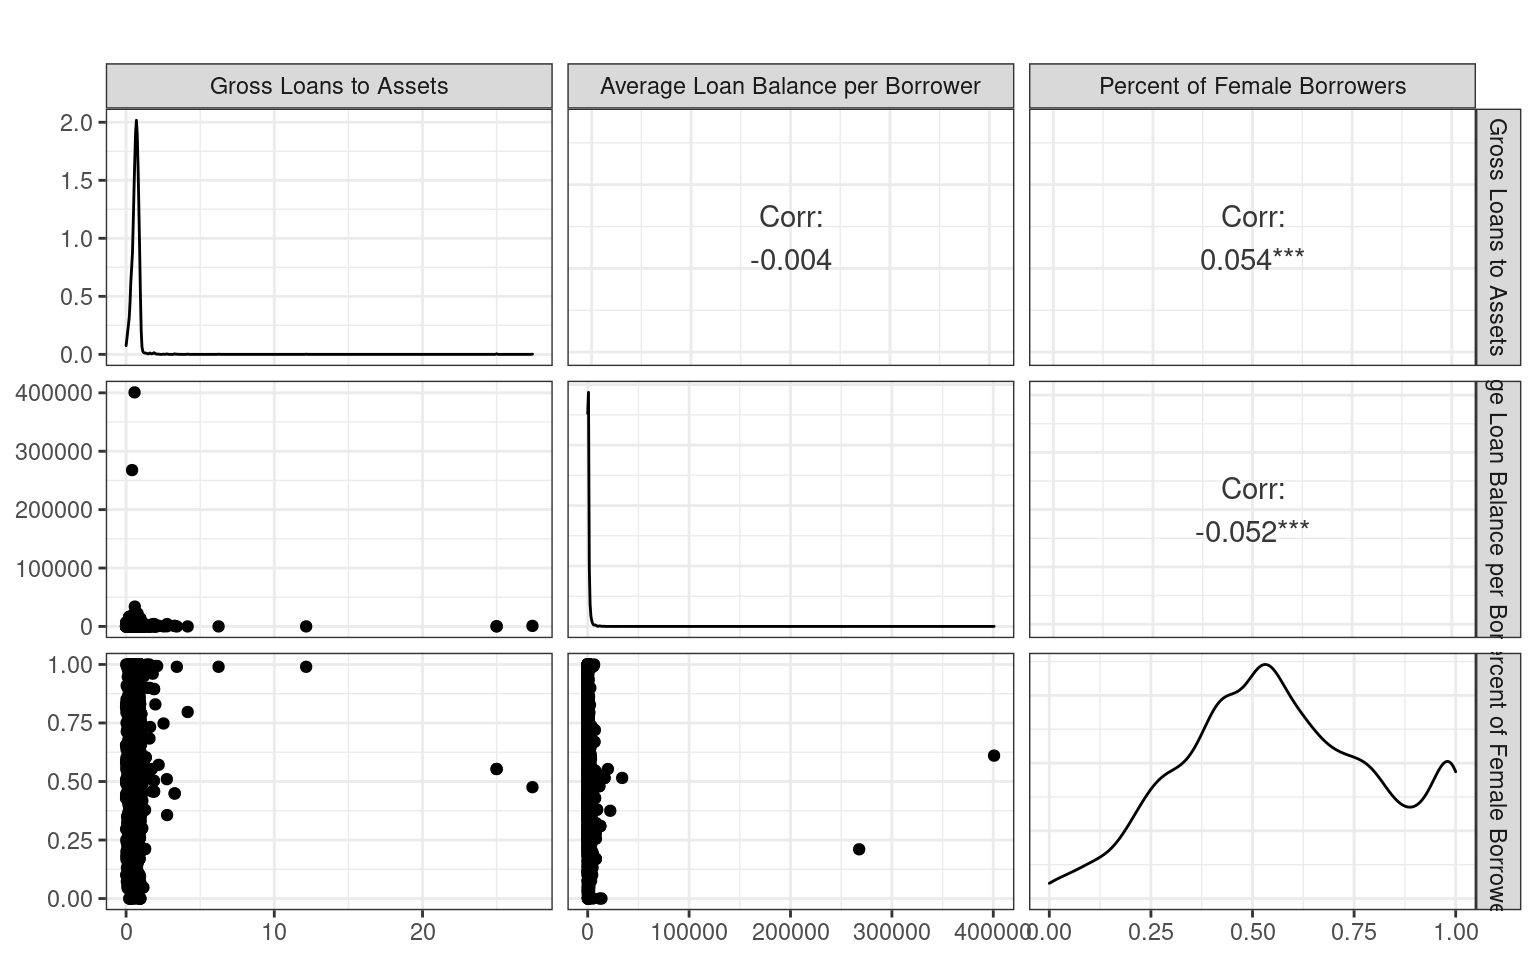
\includegraphics{_main_files/figure-latex/unnamed-chunk-87-1.pdf}
\caption{\label{fig:unnamed-chunk-87}Correlation Between Gross Loans to Assets, Average Loan Balance per Borrower, and Percent of Female Borrowers}
\end{figure}

\end{landscape}

\begin{landscape}

\newpage

\hypertarget{appendix-7-residuals-diagnostics--full-data}{%
\subsection{Appendix 7: Residuals Diagnostics- Full Data}\label{appendix-7-residuals-diagnostics--full-data}}

\begin{figure}
\centering
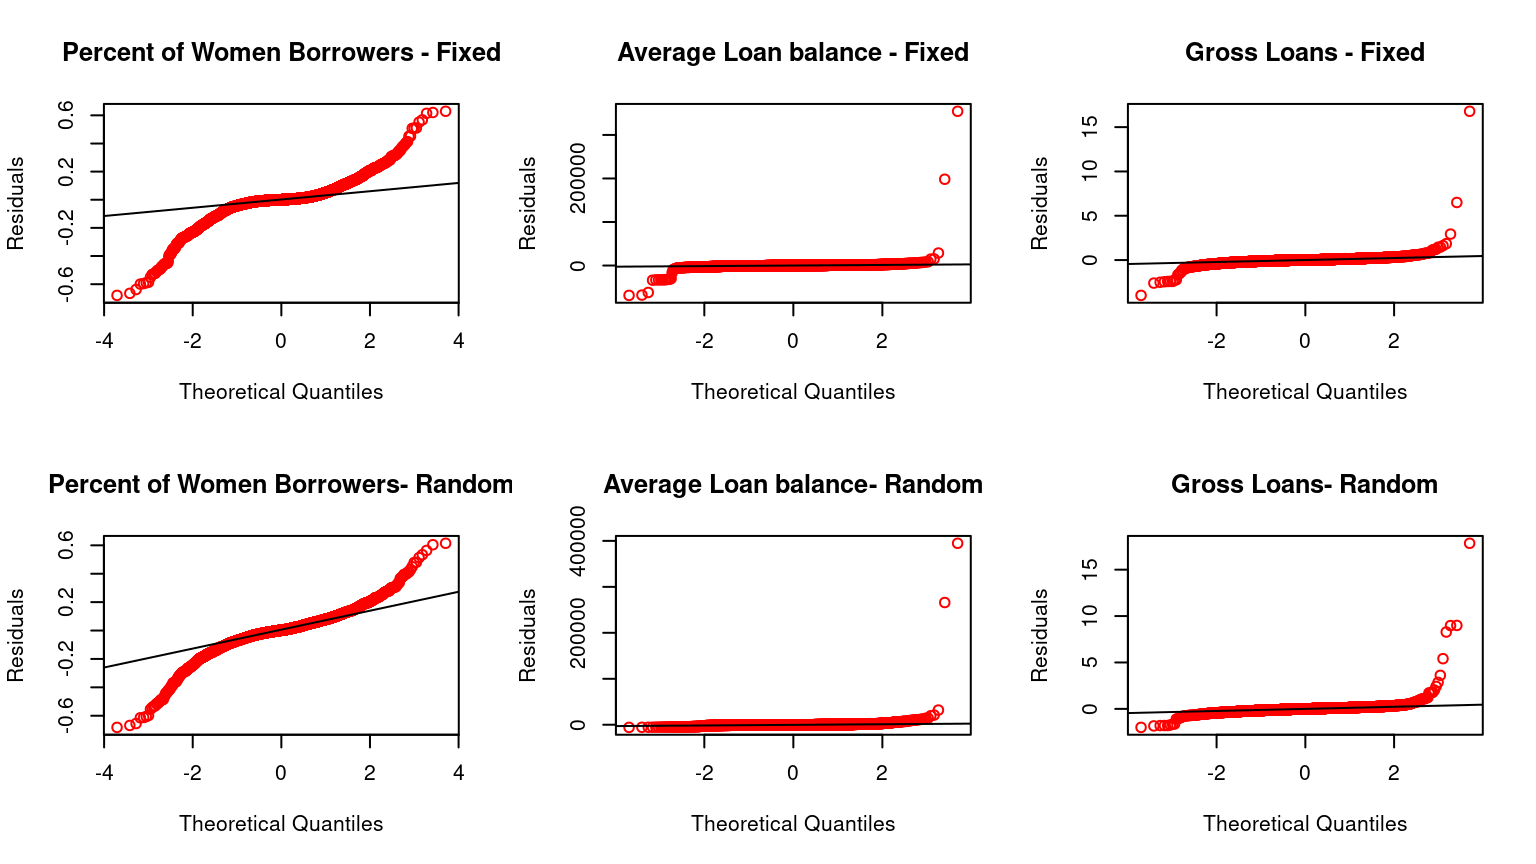
\includegraphics{_main_files/figure-latex/unnamed-chunk-88-1.pdf}
\caption{\label{fig:unnamed-chunk-88}Normal QQ Plots for the Fixed and Radom Effects Regression Models}
\end{figure}

\end{landscape}

\begin{landscape}

\newpage

\hypertarget{appendix-8-residuals-diagnostics--winsorised-data}{%
\subsection{Appendix 8: Residuals Diagnostics- Winsorised Data}\label{appendix-8-residuals-diagnostics--winsorised-data}}

\begin{figure}
\centering
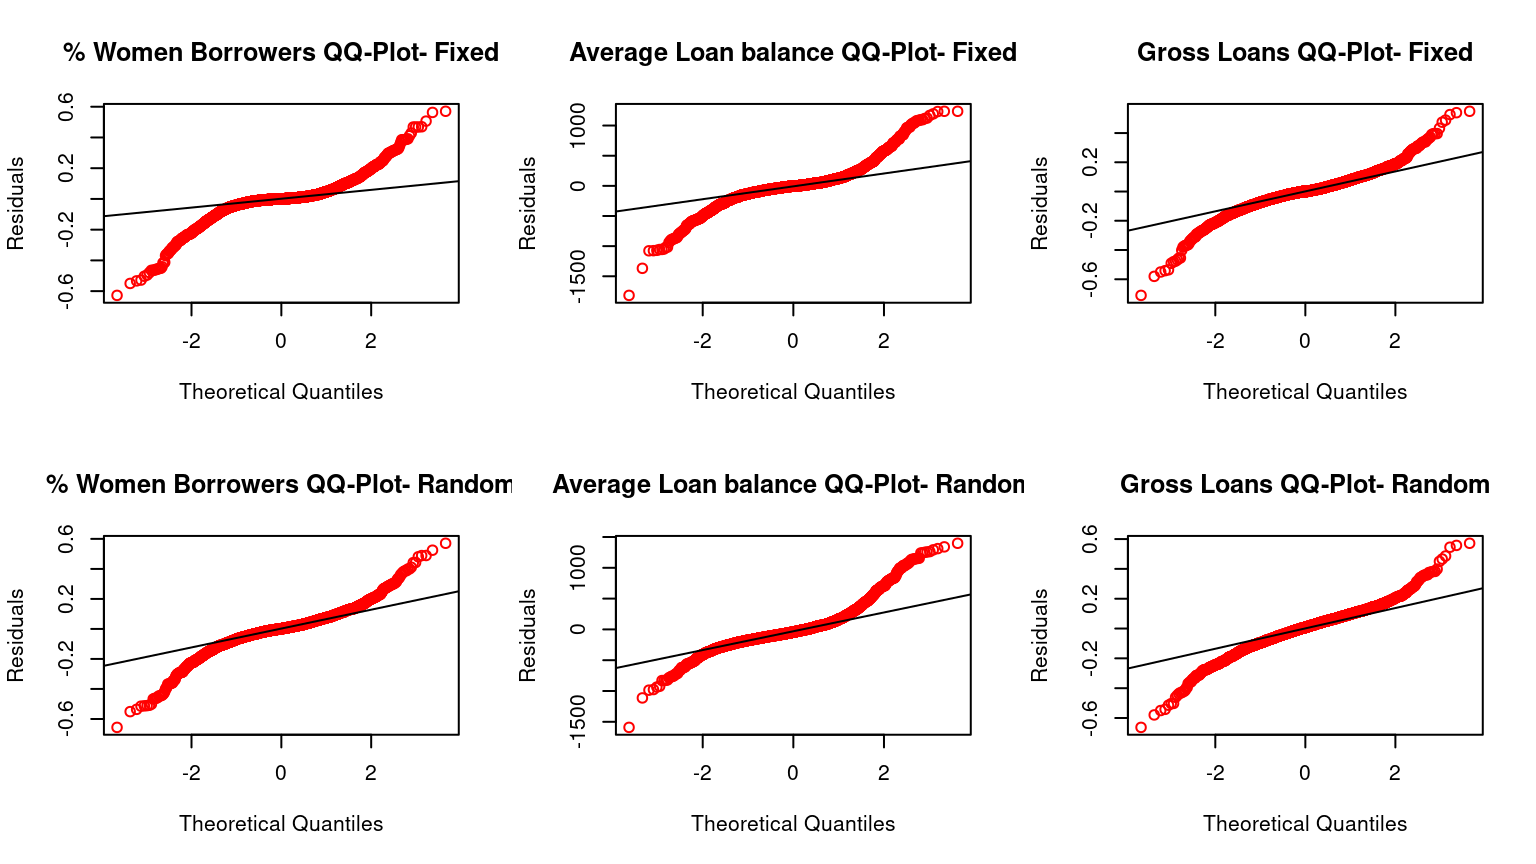
\includegraphics{_main_files/figure-latex/unnamed-chunk-89-1.pdf}
\caption{\label{fig:unnamed-chunk-89}Normal QQ Plots for Regressions Using Winsorized Data}
\end{figure}

\end{landscape}

\begin{landscape}

\newpage

\hypertarget{appendix-9-debt-to-equity-ratio-by-mfi-legal-status}{%
\subsection{Appendix 9: Debt to Equity Ratio by MFI Legal Status}\label{appendix-9-debt-to-equity-ratio-by-mfi-legal-status}}

\begin{figure}
\centering
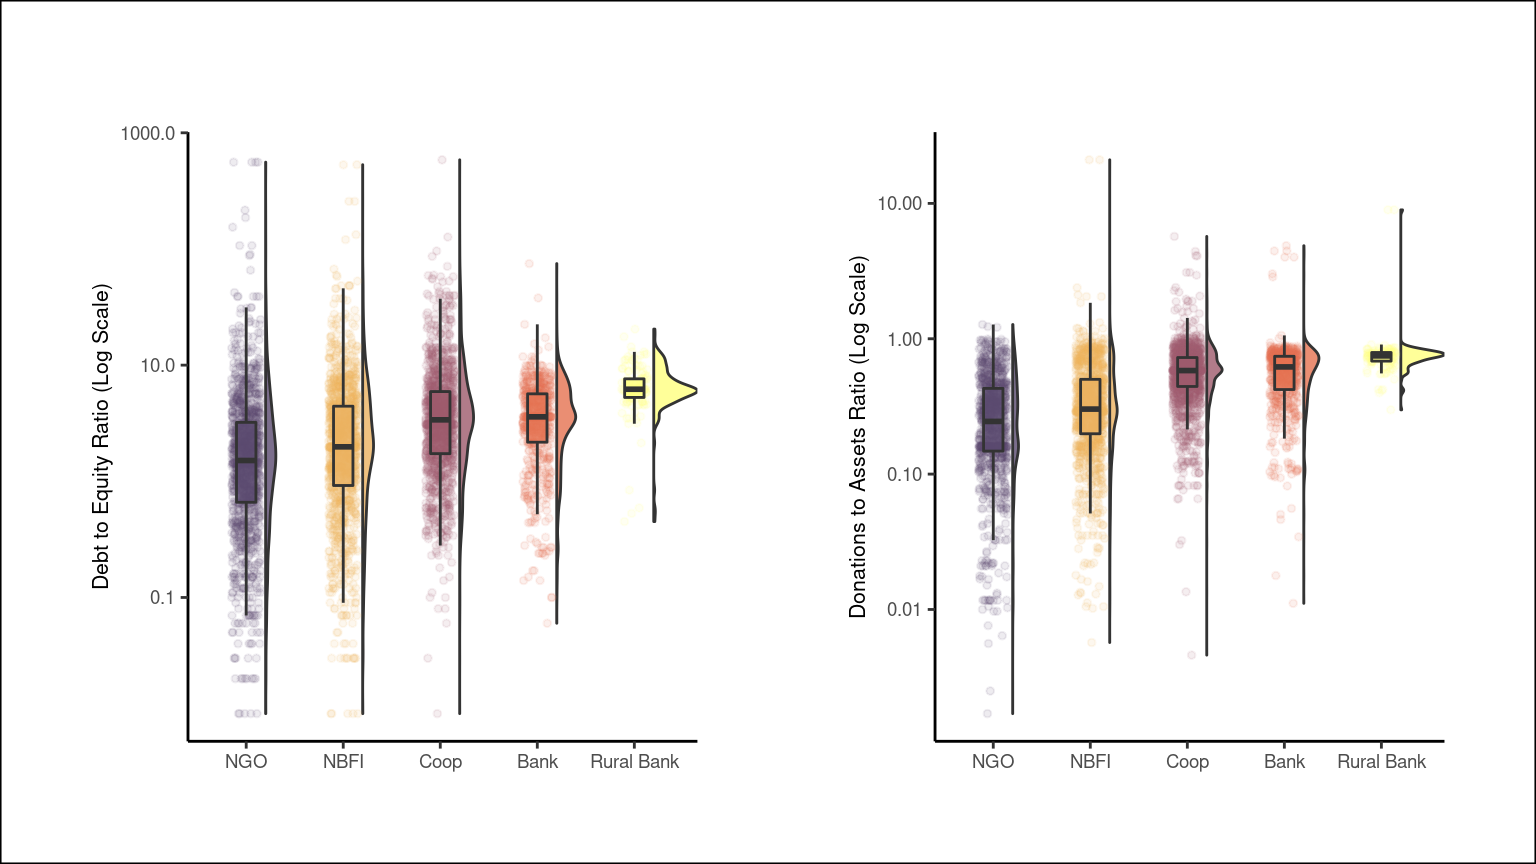
\includegraphics{_main_files/figure-latex/unnamed-chunk-90-1.pdf}
\caption{\label{fig:unnamed-chunk-90}Debt to Equity Ratio by MFI Legal Status}
\end{figure}

\end{landscape}

\begin{landscape}

\newpage

\hypertarget{appendix-10-trends-in-the-percent-of-female-borrowers}{%
\subsection{Appendix 10: Trends in the Percent of Female Borrowers}\label{appendix-10-trends-in-the-percent-of-female-borrowers}}

\begin{figure}
\centering
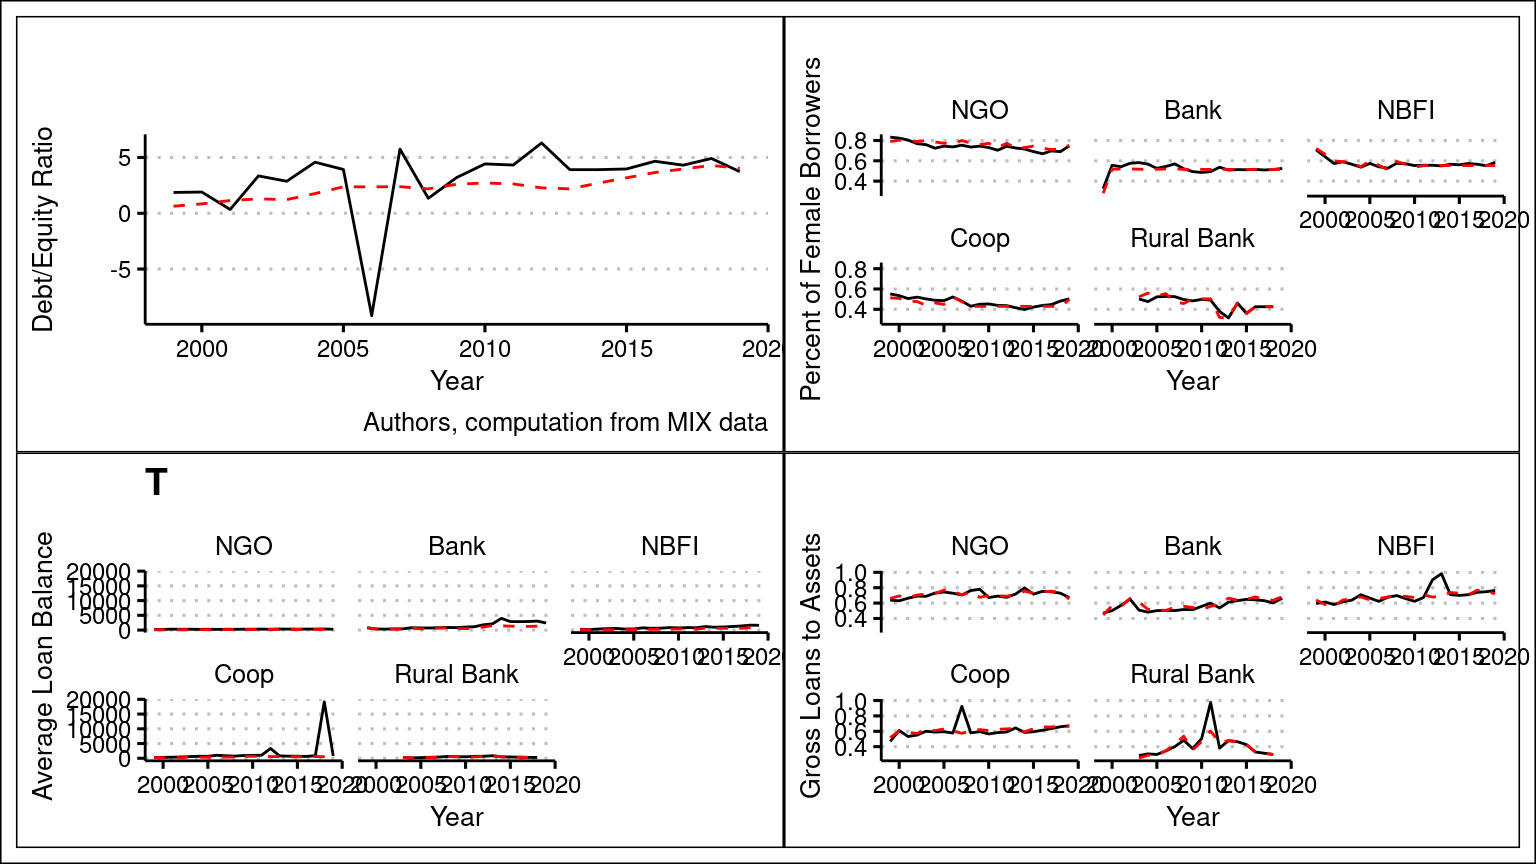
\includegraphics{_main_files/figure-latex/unnamed-chunk-91-1.pdf}
\caption{\label{fig:unnamed-chunk-91}Trends in the Percent of Female Borrowers}
\end{figure}

\end{landscape}

\hypertarget{Introduction}{%
\chapter{Efficiency of Microfinance Institutions in Africa}\label{Introduction}}

\minitoc 
\chaptermark{Efficiency of MFIs in Africa}

\newpage

\begin{center}

\textbf{ABSTRACT}

\end{center}

\begin{quote}
We use Data Envelopment Analysis (DEA) to examine the drivers, as well as levels, of financial efficiency, social efficiency, and socio-financial efficiency of microfinance institutions (MFIs) in Africa, for the period 2000-2019. Broadly, our results show a trend of declining financial efficiency but no discernible trend in both social and socio-financial efficiencies. NGO-type MFIs have markedly better social efficiency and socio-financial efficiency scores than other legal forms of MFIs. Only cooperatives and rural banks consistently outperform NGOs financially. Stock market capitalization to GDP and private credit to GDP, proxies for financial sector development, have a negative relationship with social and socio-financial efficiency and financial efficiency has an inverse relationship with both size and asset structure of MFIs. These results suggest that commercialization of MFIs does not neccesarily improve their financial sustainability. Overall, our results remain robust after excluding outliers and other checks.
\end{quote}

\vspace{10mm}

\textbf{Key Words}: Microfinance, Efficiency, Social, Financial, Performance, Africa.

\vspace{5mm}

\textbf{JEL Classification}: G210, G230

\newpage

\hypertarget{introduction}{%
\section{Introduction}\label{introduction}}

This work examines the drivers and levels of microfinance institutions (MFIs) financial and social efficiencies in Africa, considering the transformation of MFIs from not-for-profit ventures to commercial entities. Specifically, the research examines the levels and drivers of financial and social efficiencies in MFIs on the one hand. And, on the other hand, it examines the levels and drivers of the joint financial and social efficiency (socio-financial efficiency) of MFIs in Africa. MFIs have a dual mission. First, they derive legitimacy by availing financial services to the poor and other often financially excluded members of society \autocite{marconatto2016going}. To achieve this social goal, MFIs have primarily relied on private donations and government subsidies \autocite{d2017ngos}. However, with the rise of neo-liberalism \autocite{bateman2010doesn}, donors and stakeholders increasingly presume that MFIs should be financially self-sufficient, which is the second goal of MFIs \autocite{beisland2019commercialization}. Political and economic uncertainties surrounding donations and subsidies reinforce the need for MFIs to be financially independent \autocite{armendariz2011mission,garmaise2013cheap}.

If MFIs are to be financially sustainable, they should not do so by neglecting their social mission. The social mission of MFIs centres around providing appropriate and affordable financial services to the financially excluded. In Africa, the financially excluded comprises mainly women, youth and rural dwellers. When MFIs convert to the commercial model, they have to attain the financial objective of making profits and achieving financial sustainability over and above the social mission. The pursuit of financial and social goals makes MFIs hybrid organisations. It is notable, though, that purely commercial firms are also under increasing pressure to maximise social welfare primarily through corporate social responsibility (CSR) interventions and the rise of the Environmental, Social and Governance (ESG) accounting \autocite{van2016esg}, and impact investing \autocite{barber2021impact}. However, the expectation for business firms to exclusively meet social goals may not be as elevated as the expectations for social and hybrid enterprises, like MFIs. Their mission achievement is essentially predicated on fulfilling their social mandate.

In this study, we utilise Data Envelopment Analysis (DEA) to generate indices of efficiency scores for financial performance, social performance, and the joint socio-financial performance of MFIs in Africa. In examining efficiency, we focus on the extent to which MFIs optimise their output for a given level of inputs, using the output-oriented DEA approach. The alternative input-oriented approach deals with the ability of MFIs to minimise inputs for a given level of output. The choice of the output-oriented method derives from the functions of MFIs, that is, reaching out to the financially excluded sustainably. Although the optimisation of inputs is also desirable, the outputs are more relevant in this study. The DEA inputs are liabilities and equity and operating expense to assets ratio. The output metric for the financial outcome is operational self-sufficiency (OSS). Simultaneously, the average loan balance per borrower, and per cent of women borrowers, are the social performance output indicators.

This research extends existing related knowledge in three primary ways. First, the work sheds light on the determinants of the simultaneous drivers of the financial and social efficiencies of MFIs, especially in Africa, where data challenges had hitherto hindered relevant research. Secondly, as noted earlier, the paradigm shift towards the commercial approach means that MFIs should meet both financial and social objectives \autocite{d2017ngos,chahine2010social}. However, extant research on the drivers of financial and social efficiencies tends to examine each goal separately instead of viewing them as two sides of the same coin \autocite{efendic2017social,gutierrez2009social}.

What is more noteworthy is that research on the social and financial efficiency of MFIs is principally in the context of the transformation from NGOs to commercial firms and the post-conversion presence or absence of mission drift \autocite{wassie2019performance,d2017ngos,mersland2009performance,mia2017mission,ramus2017}. While some researchers find that better financial performance harms social outreach \autocite{tina2002institutional,kent2013bankers}, others find the opposite \autocite{kar2018changes,abeysekera2014sustainability}. Researchers such as \textcite{leite2019profit} find mixed outcomes, with better financial performance harming depth of outreach while improving the breadth of outreach. Therefore, by simultaneously examining both the financial and social efficiencies of MFIs, this study presents novel insights that extend the abundant literature on the financial and social performance of MFIs.

The final contribution of our work is in respect of the drivers of the social efficiency of MFIs. This contribution is paramount because it particularly informs decision making that would enhance outreach to the teeming population of the financially excluded. Researchers can, to an extent, infer the determinants of the financial performance of MFIs from insights of the numerous extant research in corporate finance. That is not the case for the social performance of MFIs and other financial institutions, for that matter. \textcite{nason2018behavioral} note that, unlike financial performance, which has specific reference points, the criterion for evaluating social performance is ambiguous. Firms must then negotiate with stakeholders on what are suitable standards for assessing social performance.

For this reason, some researchers gauge social performance by using the percentage of female borrowers, the proportion of rural borrowers, and the average loan size, all of which have their shortcomings. Much of the research in this domain dwells on the extent and causes of social failure, based on individual MFI social performance metrics without explicitly quantifying total social efficiency \autocite{lebovics2016financial,louis2013profit,louis2013financial} with the noted exception of \textcite{gutierrez2009social}. The subsequent research output based on different metrics for capturing social performance is difficult to compare.

Overall, little research investigates the socio-economic factors that enable or hinder the achievement of the dual objectives of MFIs. This absence of pertinent research is especially glaring in Africa, the continent with the lowest financial inclusion rates. For the stakeholders of MFIs, this could be a significant oversight. Therefore, the management of MFIs may not know the optimal strategies to adapt to fulfil the twin missions. The donors and venture capitalists may mistime their exit, whilst regulators could set policies that hinder rather than enhance the efficacy of MFIs in fulfilling their dual mandate. Accordingly, this research will enlighten the management of MFIs, policymakers, donors, and stakeholders on interventions necessary to enable MFIs to reach the financially excluded sustainably.

We take all formal MFIs in Africa as the population, with the sampling frame being the MFIs that submit their data to the Microfinance Information Exchange (MIX) pooled database. MIX pools data from over 2000 MFIs across the globe, representing 20\% of all formal MFIs globally, which in their assessment provide 80\% of the microcredit and incidental financial services \autocite{market2017global}. A significant issue is that a substantial number of financially excluded people often rely on informal financial services, ranging from family and friends to neighbourhood kiosks and shylocks. There is also a rise of fintech firms that use mobile phones and the internet to offer inclusive financial services. However, the data for these equally essential portions of MFIs activities is hard to capture at scale. Hence, in this study, we will rely exclusively on the MFIs listed on the MIX database.

The remainder of the research report proceeds as follows. In section 2, we review the empirical literature and describe the theoretical basis for the financial and social efficiency of MFIs. The following section provides a summary of the results of the study. Part 4 states the hypothesis and describes the empirical methods deployed in the research. Part 5 focuses on the data used in computing the efficiency scores that serve as variables in the regression. Next, Section 6 details the results and the associated robustness checks, and Section 7 concludes.

\hypertarget{theory-and-empirical-literature-1}{%
\section{Theory and Empirical Literature}\label{theory-and-empirical-literature-1}}

In \emph{Microfinance Schism}, \textcite{morduch2000microfinance} urges caution about the win-win view of microfinance. The win-win hypothesis posits that MFIs can simultaneously pursue and achieve financial sustainability and social goals without trade-offs. This perspective seeks to reconcile the welfare school of thought that views financial sustainability and social performance as incompatible and the financial sustainability perspective, which, while recognising the need for meeting social goals, emphasises financial sustainability. Morduch calls for the accommodation of multiple, hybrid MFI models on the continuum that includes those seeking profits while serving the poor and those that strictly focus on social goals like NGOs that rely on donations and subsidies. The broad array of microfinance programs, \textcite{morduch2000microfinance} argued, would then serve diverse populations and contexts instead of prioritising or rating some MF models over others \autocite{marconatto2016going}.

Nonetheless, much of the ensuing research has compared the financial sustainability model with the welfare model, with empirical support on either side \autocite{kodongo2013individual}. For instance, some research examines the extent to which different models of MFIs fare both financially and socially \autocite{abeysekera2014sustainability,bedecarrats2012combining}. Socially, ample research finds that NGO-oriented MFIs better at reaching out to the financially excluded than commercial based MFI models, that is, they are more socially efficient. However, other researchers counter that commercial oriented MFIs are better at outreach to the poor without much reliance on donations and subsidies \autocite{abeysekera2014sustainability,kar2013mission,roberts2013profit}. For instance, \textcite{dorfleitner2017microfinance}, \textcite{dorfleitner2017access}, and \textcite{bos2015practice} find that MFIs with better assets portfolio quality have a greater depth of outreach. This finding again highlights the variety of metrics used to gauge the financial and social performance of MFIs.

However, as \textcite{morduch2000microfinance} further points out, MFI social performance could depend on the segments of the population served and regional and country-level contexts. Consequently, by extension, poor and social performance definitions must expand to the different profiles and economic activities of poor people as MFIs may not effectively reach out to the ``core'' indigent. Also, the differing views on the levels of social performance could result from the diverse meanings that different stakeholders, that is, employees, managers, MFI clients, and donors, attach to the term social performance \autocite{marti2016financial}. As the metrics for social performance are ambiguous \autocite{nason2018behavioral}, it is hard to reconcile the different views of the extent to which MFIs achieve their social objectives relative to financial goals.

As a case in point, \textcite{beisland2020measuring} examine the determinants of social performance using data from social rating agencies. The researchers conclude that different rating agencies place different weights on social indicators. Nevertheless, they find financial performance, rural outreach, service quality and customer service critical determinants of MFI social performance. A related study by \textcite{hermes2018determinants} identify firm-specific and economic factors that drive the social efficiency of MFIs by conducting a meta-analysis of published papers. Key among the factors identified are age, size, institutional type, and the funding sources of an MFI, thus corroborating earlier findings by \textcite{gutierrez2009social}. However, social ratings as a measure of social performance may not be feasible in the African context, where data is challenging. Again, the importance of each indicator could vary by context. The variance motivates the need for context-specific research.

Much of the research addresses both financial performance and social performance as stand-alone without addressing the conditions under which it is possible to achieve or fail to achieve these two, respectively. \textcite{gutierrez2009social} quantified financial and social performance using the DEA efficiency estimation technique. Nonetheless, their study does not ascertain the drivers of financial efficiency, social efficiency, and combined socio-financial efficiency, as is the case in this study. Instead, these researchers examine the relationships between social performance, on the one hand, and profitability, location, age, and legal type of MFI on the other hand. This study goes beyond \textcite{gutierrez2009social} by examining the drivers of joint socio-financial efficiency and by focusing on Africa. Moreover, their data consisted of a narrower set of 89 MFIs and did not focus on a specific region for richer and potentially generalisable insights, as \textcite{d2017ngos} propose. In addition to being dated, their study also uses a notably different set of inputs and outputs data for the DEA analysis.

Hitherto, the dominant debate has been on how commercial MFIs can balance financial sustainability and social performance objectives, which attempts to mitigate the mission drift. Some researchers argue that the pursuit of financial sustainability is incompatible with outreach to the poor \autocite{cobb2016funding,mia2017mission}. The argument draws from the agency theory and its inherent profit incentive. The objectives of equity and debt holders would conflict with the strategic and costly social goal of serving the poor. It is the agency theory that forms the bedrock of arguments from the welfare school in that MFIs cannot pursue financial sustainability while at the same time reaching out to the financially excluded. These views that MFIs are likely to shift their emphasis from outreach to the poor to generate returns for the investors due to pressure from equity holders and debt servicing requirements of creditors.

\textcite{mersland2019social} also argue that restrictive covenants inherent in debt funding could push managers away from social targets to emphasise making financial returns. \textcite{armendariz2013subsidy} attribute mission drift to the need for MFIs to build up precautionary fund reserves as a cushion against uncertainties in subsidies and donations. However, other researchers like \textcite{im2015profits}, \textcite{lutzenkirchen2012microfinance}, and \textcite{quayes2012depth} argue that for transformed MFIs, mission drift cannot occur. However, \textcite{morduch2019challenges} sensibly counter this point of view by arguing that NGO MFIs would be non-existent. It is notable that NGOs that rely on donations and subsidies still form a substantial number of MFIs \autocite{armendariz2013subsidy} which to some extent validates the concern about mission drift even among funders. Despite these reservations, some works find that commercial MFIs can achieve both financial and social objectives \autocite{kodongo2013individual}. Other researchers have found that the quest for financial sustainability lowers the chances of meeting social goals \autocite{hishigsuren2006transformation}.

Further, some scholars argue that mission drift is often confused with progressive lending and cross-subsidisation \autocite{abeysekera2014sustainability}. Notable among these studies is the mission expansion thesis by \textcite{mersland2010microfinance}, which claims that financially sustainable MFIs can achieve better outreach through cross-subsidisation, that is, lending at market rates to the relatively well-off and using the proceeds to subsidise interest payments for the poor. Interestingly, \textcite{campion1999institutional} and \textcite{ramus2017} argue that mission expansion could occur not due to the commercialisation of MFIs but due to a failure of corporate governance. Hence, corporate governance could resolve mission drift without affecting the financial positioning or social orientation of an MFI.

Lastly, a closely related study by \textcite{lam2020reciprocity} finds that MFIs exhibit no evidence of mission drift. Instead, they find that financial performance is positively associated with subsequent social performance in for-profit MFIs relative to not-for-profit MFIs. Moreover, in contrast, the social performance of not-for-profit MFIs varies positively with subsequent financial performance compared to for-profit MFIs. Therefore, these authors surmise that for-profit MFIs are more efficient at translating financial performance to social goals while nonprofits are better at translating social objectives to financial goals. For nonprofits, part of the reason could be the goodwill generated by meeting social goals, which leads to more support from donors, the state, and other stakeholders. MFIs that are profit-based, however, must first generate profit to enable them to address social goals.

\hypertarget{hypotheses}{%
\section{Hypotheses}\label{hypotheses}}

While the highlighted studies examine efficiency aspects separately, this study goes further by looking into the collective social and socio-financial and performance. Hence, in addition to reviewing the drivers of financial and social efficiencies of MFIs, we hypothesise, in positive format, as follows.

\begin{itemize}
\tightlist
\item
  Hypothesis 1: MFIs that follow the commercial model exhibit better financial performance than MFIs that follow the NGO model.
\item
  Hypothesis 2: The social performance of NGO based MFIs is better than that of commercial model based MFIs.
\item
  Hypothesis 3: The joint socio-financial performance of NGO based MFIs is better than that of commercial model based MFIs.
\end{itemize}

In these hypotheses, we note that most NGOs are also shifting to the commercial model but continue to rely substantially on donor funds, government subsidies, and guarantees to access low-cost commercial funds \autocite{d2013unsubsidized}. Further, the mission of NGO-type MFIs may defer markedly from that of commercial MFIs, meaning that even when pursuing profits, they are less likely to abandon the social goals \autocites{louis2013profit}[@][]{mersland2019social}. The section that follows summarises the results of this current study.

\hypertarget{summary-of-results-2}{%
\subsection{Summary of Results}\label{summary-of-results-2}}

This section highlights the results of the data analysis on the levels and drivers of social efficiency, financial efficiency, and combined socio-financial efficiency of MFIs in Africa. The section also elucidates our hypothesised relations vis-a-vis MFI types. The inputs for the DEA analysis constitute measures for financial performance and social performance. We capture financial performance using operational self-sufficiency (OSS). For social performance, we use two metrics; the per cent of women borrowers and the average loan balance per borrower. These metrics capture the ability of MFIs to reach the most financially excluded people such as women, rural dwellers, and other people that require and would typically make do with small loans sizes. The discussion captures the individual inputs and overall DEA score that researchers have documented in the literature.

MFIs in Africa are barely financially sustainable, with marginal disparities between MFIs legal types. On a scale between zero and one, the mean and median financial efficiency scores are 0.1572 and 0.1079, respectively. The regression analysis shows that the asset structure and size of an MFI are the primary drivers of financial efficiency. Larger MFIs have lower financial efficiency scores, as do MFIs with a higher assets structure (this is the ratio of non-current assets to total assets). MFIs exhibit a high level of social efficiency, consistent with their mission of providing financial services to the financially excluded, mostly the poor. The mean and median social efficiency scores are 0.786 and 0.777, respectively. The socio-efficiency scores are equally high. NGOs have significantly higher social efficiency and socio-financial efficiency scores than other legal forms of MFIs. The key driver of social efficiency and socio-financial efficiency is the MFI legal status. Financial markets development, proxied by stock market capitalisation to GDP and private credit to GDP, relate negatively to social efficiency and socio-financial efficiency. The following section lays out the methodology.

\hypertarget{methodology-and-data}{%
\section{Methodology and Data}\label{methodology-and-data}}

The study adopts a quantitative approach with the empirical model specified next.

\hypertarget{the-empirical-model}{%
\subsection{The Empirical Model}\label{the-empirical-model}}

We primarily use the fixed and random-effects models as per the result of the Hausman test (see Appendix 1). Specifically, we estimate the following model.

\begin{equation}
Y_{it} = \beta_{0} + \beta_{1}X_{it} + \mu_{it}
\end{equation}

Further, assume that,

\begin{equation}
\mu_{it} = C_{i} + \epsilon_{it}
\end{equation}

Where \(Y_{it}\) represents the dependent variable, which takes efficiency scores derived from the data envelopment analysis (DEA) model. We compute three measures of efficiency that take turns as the dependent variables: social efficiency, financial efficiency, and socio-financial efficiency. Section 5.4.3 describes in detail the DEA model.

\(X_{it}\), on the other hand, represents the set of independent variables as described in Table 4.2 below. Further, \(c_{i}\) captures the aggregate effects of the unobserved, time-invariant explanatory variables for \(Y_{it}\) . Further, assume that \(e_{it}\) has zero mean conditional on \(X_{it}\). In the case where \(C_{i}\) and \(X_{it}\) are correlated, then \(C_{t}\) is a fixed effect; otherwise, it is a random effect. Note that the existence of fixed effects implies the presence of endogeneity. For random effects, on the other hand, endogeneity is not a concern. However, the random-effects model affects the computation of standard errors \autocite{roberts2013endogeneity}.

\hypertarget{data-data-sources-and-description-of-variables.}{%
\subsection{Data, Data Sources and Description of Variables.}\label{data-data-sources-and-description-of-variables.}}

We source our data from the Microfinance Information Exchange (MIX) pooled database \footnote{The MIX Market database is available on this link \url{https://datacatalog.worldbank.org/dataset/mix-market}.}, the World Development Indicators (WDI) \footnote{The link to the WDI database is \url{https://databank.worldbank.org/source/world-development-indicators}.}, the Global Financial Development Database (GFDD) \footnote{The link to the GFDD is \url{https://www.worldbank.org/en/publication/gfdr/data/global-financial-development-database}.}, and the Worldwide Governance Indicators (WGI) \footnote{Follow the link for more information about the WGI, \url{https://info.worldbank.org/governance/wgi/}.}. The dataset used in this article consists of 705 MFIs across Africa. While the MIX data is not a comprehensive representation of the microfinance industry in Africa, it does provide general trends in the sector \autocite{jarotschkin2013microfinance}.

\hypertarget{the-dea-model}{%
\subsection{The DEA Model}\label{the-dea-model}}

As noted earlier, the study adopts the Data Envelopment Analysis (DEA) technique to estimate both the financial and social efficiency scores for a given MFI in each period. \textcite{charnes1978measuring} and \textcite{charnes1981evaluating} formulated the traditional data envelopment analysis (DEA) by following the ideas of \textcite{farrel1957measurement}. Unlike the other measures of financial and social performance of MFIs, DEA quantifies the (inverse) agency costs without confounding factors unrelated to agency costs \autocite{berger2006capital}. A significant advantage of DEA is that it is not prone to the standard econometric problems because it is a deterministic and non-parametric enveloping technique. For instance, in running the DEA model, the researcher does not have to specify a functional form, estimate parameters, or define an error term. Importantly, DEA makes no distinction between dependent and independent variables \autocite{zhou2007non}.

DEA requires the resolution of the following linear programming model.

\begin{equation}
\frac{\sum_{r=1}^{n} u_{r}v_{r}}{\sum_{i=1}^{m} v_{i}x_{i}} \leqslant 1
\end{equation}

\begin{equation}
for, u_{r}, v_{r} \geqslant 0
\end{equation}

In this case, \(n\) is the output number while \(m\) is the input number. Also, \(u_{r}\) is the weight of n, and \(v_{i}\) is the weight of m. Hence, \(v_{i}\) and \(x_{i}\) represent the weight of m and output of \(m\), respectively. Similarly, \(u_{r}\) and \(v_{r}\) represent the weight and amount of input in that order.

When researchers run DEA assuming constant returns to scale (CRS), the resulting output represents technical efficiency (TE). Technical efficiency stands for the efficiencies due to input-output configurations and the size of operations. Under variable returns to scale, the output is pure technical efficiency (PTE). PTE is the efficiency that arises from input-output configuration while ignoring the scale of operations \autocite{staub2010evolution,ulas2015performance}. Additionally, input-oriented DEA seeks to minimise inputs for a given level of output, while in the case of output-oriented DEA, the goal is to maximise outcomes for a given level of inputs, with the choice of the orientations based on the input or output variables that managers have the most control over \autocite{huguenin2012data}.

\hypertarget{inputs-and-outputs-for-the-dea-model}{%
\subsubsection{Inputs and Outputs for the DEA Model}\label{inputs-and-outputs-for-the-dea-model}}

In this section, we first describe the inputs and outputs for the DEA efficiency model. We derive the efficiency scores from the Data Envelopment Analysis (DEA) model, where each of the MFIs is a decision-making unit (DMU) that converts multiple inputs into outputs. The efficiency scores show the relative annual configuration of inputs and outputs per MFI in the sample, as listed below. The output from the DEA forms the dependent variables. After describing the inputs and outputs for the DEA model, we describe the independent variables for the regression analysis.

\hypertarget{inputs-for-the-dea-efficiency-scores}{%
\paragraph{Inputs for the DEA efficiency scores:}\label{inputs-for-the-dea-efficiency-scores}}

Following the intermediation approach, we use the following variables as inputs.

\begin{itemize}
\item
  Liabilities and equity to total assets ratio: Liabilities and equity, an equivalent of total assets, capture all the funding sources for the MFI, including debt, equity, deposits, donations, and subsidies at the end of the reporting period. Liabilities and equity is a prominent input for DEA analysis, for instance, in studies on efficiency summarised by \textcite{fethi2010assessing}, \textcite{paradi2017data}, and \textcite{fall2018dea}.
\item
  Operating expenses to total assets ratio: This ratio captures the portion of assets per annum used to fund the operations of the MFI that directly generates the financial and social outputs described next. Staff numbers are the primary input in several DEA models. In this study, we take operating costs by subsuming the number of staff into labour cost.
\end{itemize}

\hypertarget{outputs-for-the-dea-efficiency-scores}{%
\paragraph{Outputs for the DEA efficiency scores:}\label{outputs-for-the-dea-efficiency-scores}}

We classify outputs in both financial and social terms. Social outputs proxy the extent to which MFIs avail financial services to the poor and the financially excluded. Other outputs measure financial sustainability by MFIs. Accordingly, outputs consist of the following variables;

\emph{Social Performance outputs}:

\begin{itemize}
\tightlist
\item
  Depth Measures: Percent of female borrowers and average loan size per borrower: The percentage of women borrowers as a measure of social efficiency draws from the fact that women form the bulk of the impoverished population and are financially excluded. Researchers have used the average loan size to proxy social performance as poor people will often borrow small amounts regularly to run their businesses and settle bills. In this case, the lower the average loan balance per borrower, the deeper the outreach \autocite{d2017ngos}.
\end{itemize}

\emph{Financial Performance outputs}:

\begin{itemize}
\tightlist
\item
  Operational self-sufficiency (OSS): OSS 1 captures the extent to which an MFI meets its financial objectives by generating financial returns that can cover all the expenses. MIX defines the OSS as follows;
\end{itemize}

\begin{equation}
OSS1 = \frac{Operating Revenue}{Expenses on Funding, Loan Loss Provisions, and Operations}
\end{equation}

OSS 1 has an advantage over OSS 2, which only shows the extent to which an MFI can cover its operating costs. We utilise OSS 1 in the study.

\begin{equation}
OSS2 = \frac{Operating Revenue}{Operating Expenses}
\end{equation}

Table 4.1 presents summary statistics for the DEA input and output variables.

\begin{table}

\caption{\label{tab:unnamed-chunk-109}Summary Statistics: Inputs and Outputs for the DEA Model}
\centering
\fontsize{9}{11}\selectfont
\begin{tabular}[t]{lrrrrrr}
\toprule
Variable & Mean & SD & Q1 & Median & Q3 & Max\\
\midrule
Liabilities/Equity & 44716574.639 & 330693249.176 & 584257.000 & 2617933.000 & 13218887.000 & 9538256131.00\\
Operating Expense/Assets & 0.227 & 0.185 & 0.124 & 0.181 & 0.269 & 2.52\\
Female borrowers (\%) & 0.569 & 0.237 & 0.421 & 0.550 & 0.748 & 1.00\\
Average Loan & 867.531 & 7094.479 & 150.250 & 351.000 & 724.000 & 400764.00\\
Gross Loans/Assets & 0.655 & 0.704 & 0.507 & 0.654 & 0.775 & 27.42\\
\bottomrule
\multicolumn{7}{l}{\rule{0pt}{1em}Source: Authors construction from the data}\\
\end{tabular}
\end{table}

Before running the DEA analysis, we start by transforming the inputs and outputs. We add a significantly large number to eliminate zeros and negatives \autocite{ataullah2006economic}. In line with \textcite{avkiran2006productivity}, we also mean-normalize the data. Figure 5.1 shows that there is a very low correlation between the inputs and outputs. Hence, collinearity will not adversely affect the DEA scores.

\hypertarget{independent-variables}{%
\subsection{Independent Variables}\label{independent-variables}}

Table 4.2 presents a summary of the independent variables applied in the study \footnote{See \textcite{jensen1976theory}, \textcite{titman1988determinants}, \textcite{ledgerwood1998microfinance}, \textcite{kyereboah2007determinants}, \textcite{kraay2010worldwide}, \textcite{allen2014african}, \textcite{kurshev2015firm}, \textcite{bayai2016financing}, \textcite{schnyder2018twenty}, \textcite{kimmel2018financial}, \textcite{ito2018quantity}, \textcite{market2018global}}.

\begin{table}

\caption{\label{tab:unnamed-chunk-110}Description of Independent Variables}
\centering
\fontsize{9}{11}\selectfont
\begin{tabu} to \linewidth {>{\raggedright}X}
\toprule
Variable\_Description\\
\midrule
1. Current Legal Status: The legal forms of registration of an MFI are as follows: Commercial Bank, Non-Bank Financial Institution (NBFI), Non-Governmental Organization (NGO), Credit Union/ Cooperative, or Rural Bank. The legal status may dictate the profit orientation and sources of capital for the MFIs. We hypothesize that NGOs have better social performance measures while commercial MFIs have better financial outcomes\\
\\
2.  Age: MIX classifies MFIs into three categories depending on the time that has elapsed since the MFI started operations - new (0-4 years), young (4-8 years) and mature (over eight years). The variable is hence a dummy. We hypothesise that older, and hence larger MFIs, are more likely to be more efficient given they can draw from economies of scale, hire better managers, and have a long experience in running microfinance programs.\\
\\
3. Size (Log of Total Assets): We proxy the size of MFI with the natural logarithm of total assets, again using MIX data. Assets are supported by the sum of capital and liabilities or, equivalently, the total value of resources owned or controlled by the MFI resulting from past and current activities and from which the MFI derives future benefits. We propose that larger firms should be more efficient due to economies of scale and scope.\\
\addlinespace
\\
4. Governance/ Institutional Quality (KKM): We create the country level KKM index using the first principal component of the WGI available in the World Bank databases. The index captures the institutional quality via corruption control, government effectiveness, political stability, the rule of law, and voice and accountability (Kaufmann, Kraay, \& Mastruzzi, 2011). The proposition is that MFIs located in countries with better governance are also likely to have better internal governance which translates to better financial and social performance. We use the terms institutional quality and governance interchangeably throughout the text.\\
\\
5. Private Credit to GDP: We capture the total amount of credit advanced to the private sector by financial intermediaries as a proxy for capital markets development concerning the banking sector following Ito and Kawai (2018). The data source is the Global Financial Development Database, GFDD, of the World Bank (See note 4). Private credit to GDP represents the financial resources provided to the private sector by domestic money banks as a share of GDP. Domestic money banks comprise commercial banks and other financial institutions that accept transferable deposits, such as demand deposits. The data is available in WDI. Financial sector development is central to the acquisition of both equity and debt financing. We hypothesise that a high private credit to GDP corresponds with lower financial and social outcomes for MFIs given the relatively low levels of financial exclusion in countries with well developed financial systems.\\
\\
\addlinespace
6. Stock market capitalisation to GDP: We capture the extent of stock market development using the ratio of stock market capitalisation to GDP to proxy the ease by which firms can raise equity capital. Although Africa's equity markets are thin, some relatively large stock markets like South Africa, Egypt, Nigeria, Kenya, and Ghana exist. The data are from the GFDD. We hypothesize that MFIs located in countries with better stock markets development have lower financial and social performance given the low levels of financial exclusion. It means that MFIs have to compete with mainstream financial intermediaries.\\
\\
7. Asset Structure (Tangibility): Asset structure is measured as the ratio of non-current assets to total assets of an MFI (Microfinance Information Exchange (MIX), 2019). The percentage indicates the extent of investment in physical infrastructure, a significant issue in constraining banking for the poor due to the perceived lack of scale economies to warrant the erection, for instance, of brick and mortar branches (Ledgerwood, 1998). Firms with a lower ratio are likely to release more funds for lending and hence better social and financial performance. (Titman \& Wessels, 1988; Kyereboah-Coleman, 2007a).\\
\\
\bottomrule
\multicolumn{1}{l}{\rule{0pt}{1em}\textit{Source: }}\\
\multicolumn{1}{l}{\rule{0pt}{1em}Authors' construction from the literature}\\
\multicolumn{1}{l}{\rule{0pt}{1em}\textit{Notes}}\\
\multicolumn{1}{l}{\rule{0pt}{1em}\textsuperscript{1} MIX Database on www.themix.org and https://datacatalog.worldbank.org/dataset/mix-market}\\
\multicolumn{1}{l}{\rule{0pt}{1em}\textsuperscript{2} WDI on https://databank.worldbank.org/source/world-development-indicators.}\\
\multicolumn{1}{l}{\rule{0pt}{1em}\textsuperscript{3} WGI/ KKM on https://databank.worldbank.org/source/worldwide-governance-indicators.}\\
\multicolumn{1}{l}{\rule{0pt}{1em}\textsuperscript{4} GFDD on https://www.worldbank.org/en/publication/gfdr/data/global-financial-development-database}\\
\end{tabu}
\end{table}

\begin{landscape}

\newpage

\begin{figure}
\centering
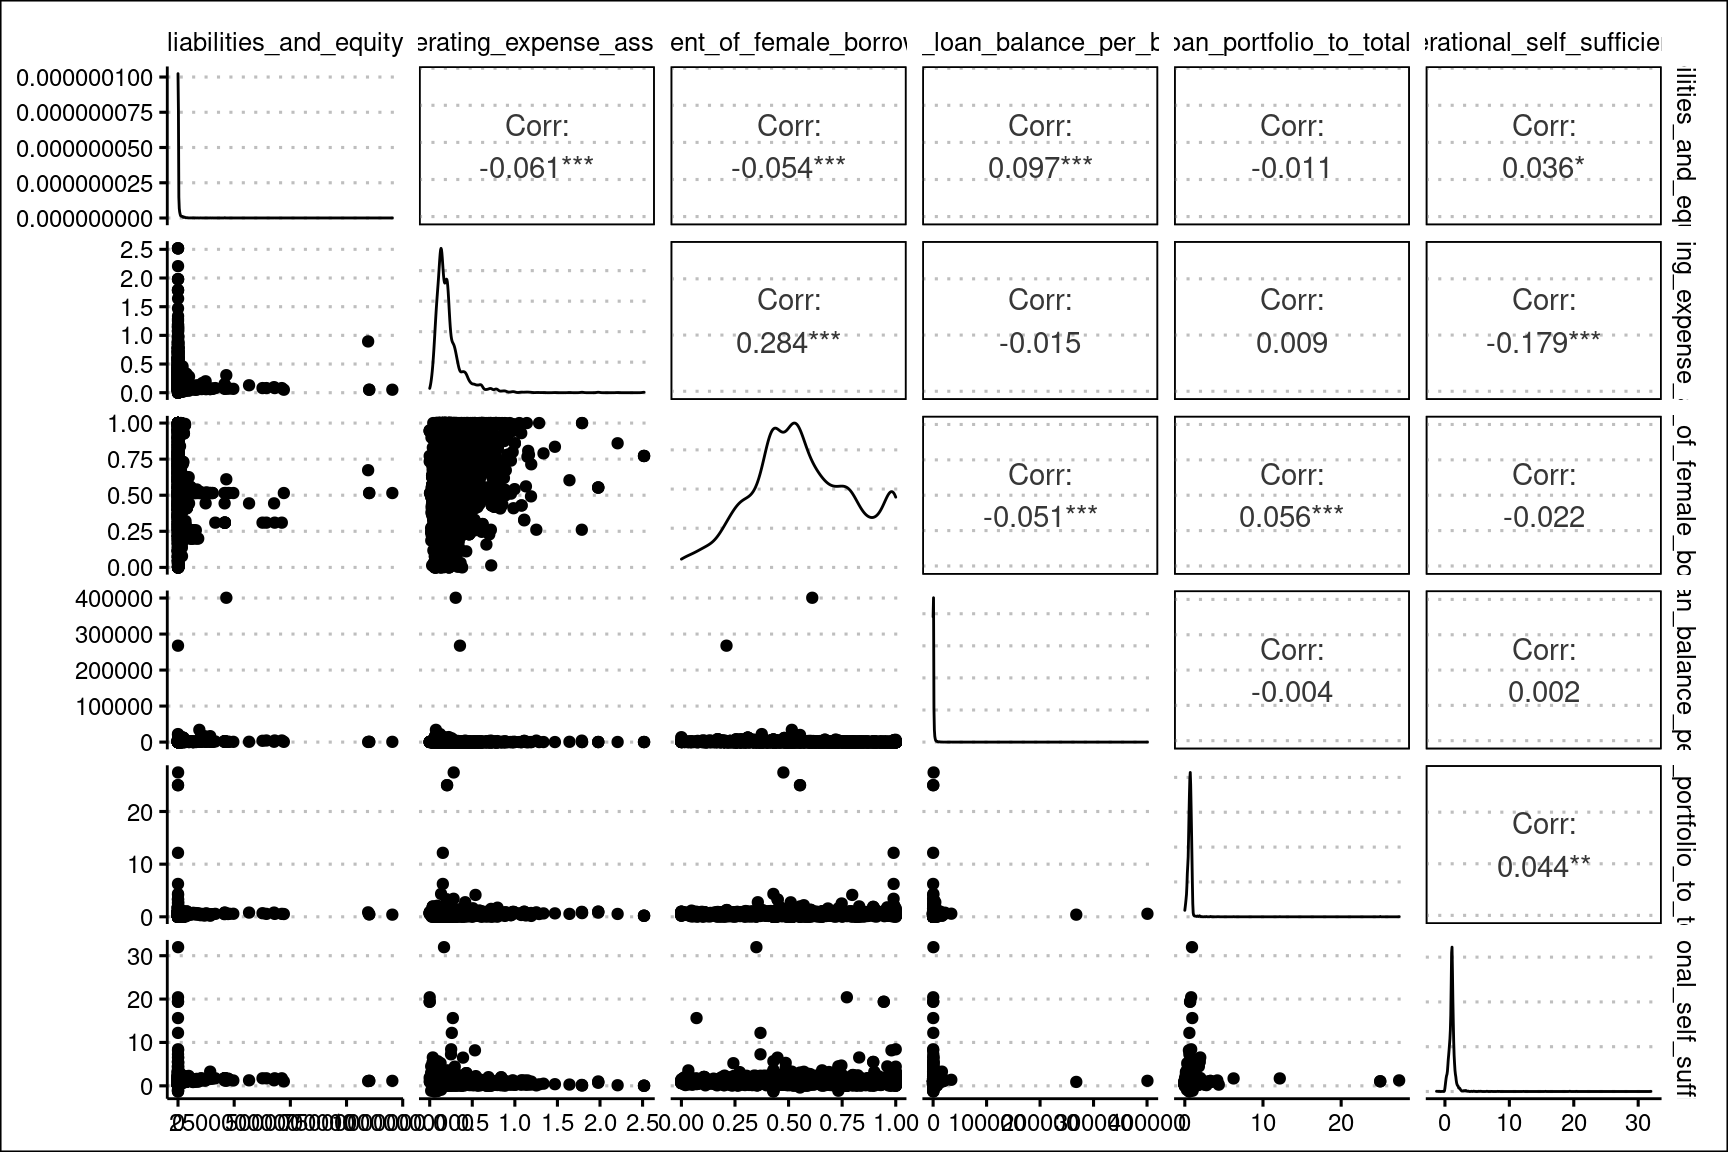
\includegraphics{_main_files/figure-latex/unnamed-chunk-111-1.pdf}
\caption{\label{fig:unnamed-chunk-111}Correlation Matrix for DEA Inputs and Outputs}
\end{figure}

\end{landscape}

\newpage

\hypertarget{results-1}{%
\section{Results}\label{results-1}}

Recall, we examine the indicators of financial and social performance by MFIs in Africa. Here, we focus on taking individual performance measures, the proportion of female borrowers, average loan balance per borrower, gross loans to assets, and operational self-sufficiency. While the examination of indicator variables does not explicitly measure efficiency (we do this in a later section using DEA), they illustrate the extent to which MFIs fare in their mission more broadly:

\begin{enumerate}
\def\labelenumi{\arabic{enumi}.}
\tightlist
\item
  Table 4.3 presents the descriptive statistics for the DEA-based efficiency scores. We visualise the data and describe the scope of financial and social performance, followed by a discussion of the DEA efficiency scores.
\item
  We discuss the levels of efficiency by MFI types based on the DEA scores.
\item
  We summarise the independent variables employed in the subsequent regression models.
\item
  We layout and describe the results of the regression model.
\end{enumerate}

\hypertarget{dea-efficiency-scores}{%
\subsubsection{DEA Efficiency Scores}\label{dea-efficiency-scores}}

Given that the model is output-oriented, the interpretation is as follows: given a set of inputs, to what extent are MFIs able to maximise output? Given that the study targets the degree of financial inclusion and financial sustainability of MFIs, the maximisation of outcomes is more relevant for this study.

\hypertarget{financial-efficiency}{%
\paragraph{Financial Efficiency}\label{financial-efficiency}}

The mean and median financial efficiency scores are 0.16 and 0.11, respectively \footnote{The DEA scores range between zero and one, with zero indicating the worst performance and one the best.}. Taken together with Figure 5.2, the results show that the financial efficiency scores skew heavily to the right. Critically, MFIs are hardly financially sustainable regardless of their legal form, despite the paradigm shift towards commercialization. This observation begs the following two questions: do commercially oriented legal forms of MFI perform better financially than NGO-type MFIs? Further, do newer MFIs that took root when donors emphasize the financial sustainability of MFIs do better financially than older MFIs?

Figure 5.2, panel C shows that only cooperatives and rural banks have higher median financial efficiency scores than NGOs. These results do not support the supposition that commercialization raises financial sustainability, given that commercial banks and NBFIs fare worse financially. The poor financial performance by banks and NBFIs can only further worsen their outreach to the financially excluded. Besides, the poor financial performance is also contrary to the ``mission expansion'' hypothesis where commercial MFIs generate profits that they then use to reach more financially excluded clients. Furthermore, Figure 5.2, panel D shows that newer MFIs have higher financial sustainability scores relative to older MFIs. These results could mean that newer MFIs focus more on financial sustainability at the expense of social goals or are better at balancing financial sustainability with social goals.

Figure 5.5, panel B shows the trends in median financial efficiency scores of MFIs for 1999-2020. Cooperatives consistently do better financially than other legal forms. Surprisingly, NGOs and rural banks follow, while NBFIs and commercial banks have the lowest median financial efficiency scores, with commercial banks showing wide variability. The results indicate that commercialization does not necessarily raise financial sustainability, especially in the absence of grants and state subsidies. What is concerning is the observation that financial efficiency is on a downward spiral, meaning that MFIs may not achieve the goal of financial sustainability of MFIs. The worsening trend in financial performance by MFIs may point to the harm that neo-liberalism, commercialization, or other unidentified macro-economic factors have on MFIs.

\begin{table}

\caption{\label{tab:unnamed-chunk-112}Summary Statistics for Efficiency Scores}
\centering
\fontsize{9}{11}\selectfont
\begin{tabular}[t]{lrrrrrrr}
\toprule
Variable & Mean & SD & Min & Q1 & Median & Q3 & Max\\
\midrule
financial Efficiency & 0.157 & 0.189 & 0.029 & 0.094 & 0.108 & 0.127 & 1\\
Social Efficiency & 0.786 & 0.119 & 0.500 & 0.713 & 0.777 & 0.875 & 1\\
Social-Financial Efficiency & 0.795 & 0.123 & 0.500 & 0.715 & 0.777 & 0.894 & 1\\
\bottomrule
\end{tabular}
\end{table}

\begin{landscape}

\newpage

\begin{figure}
\centering
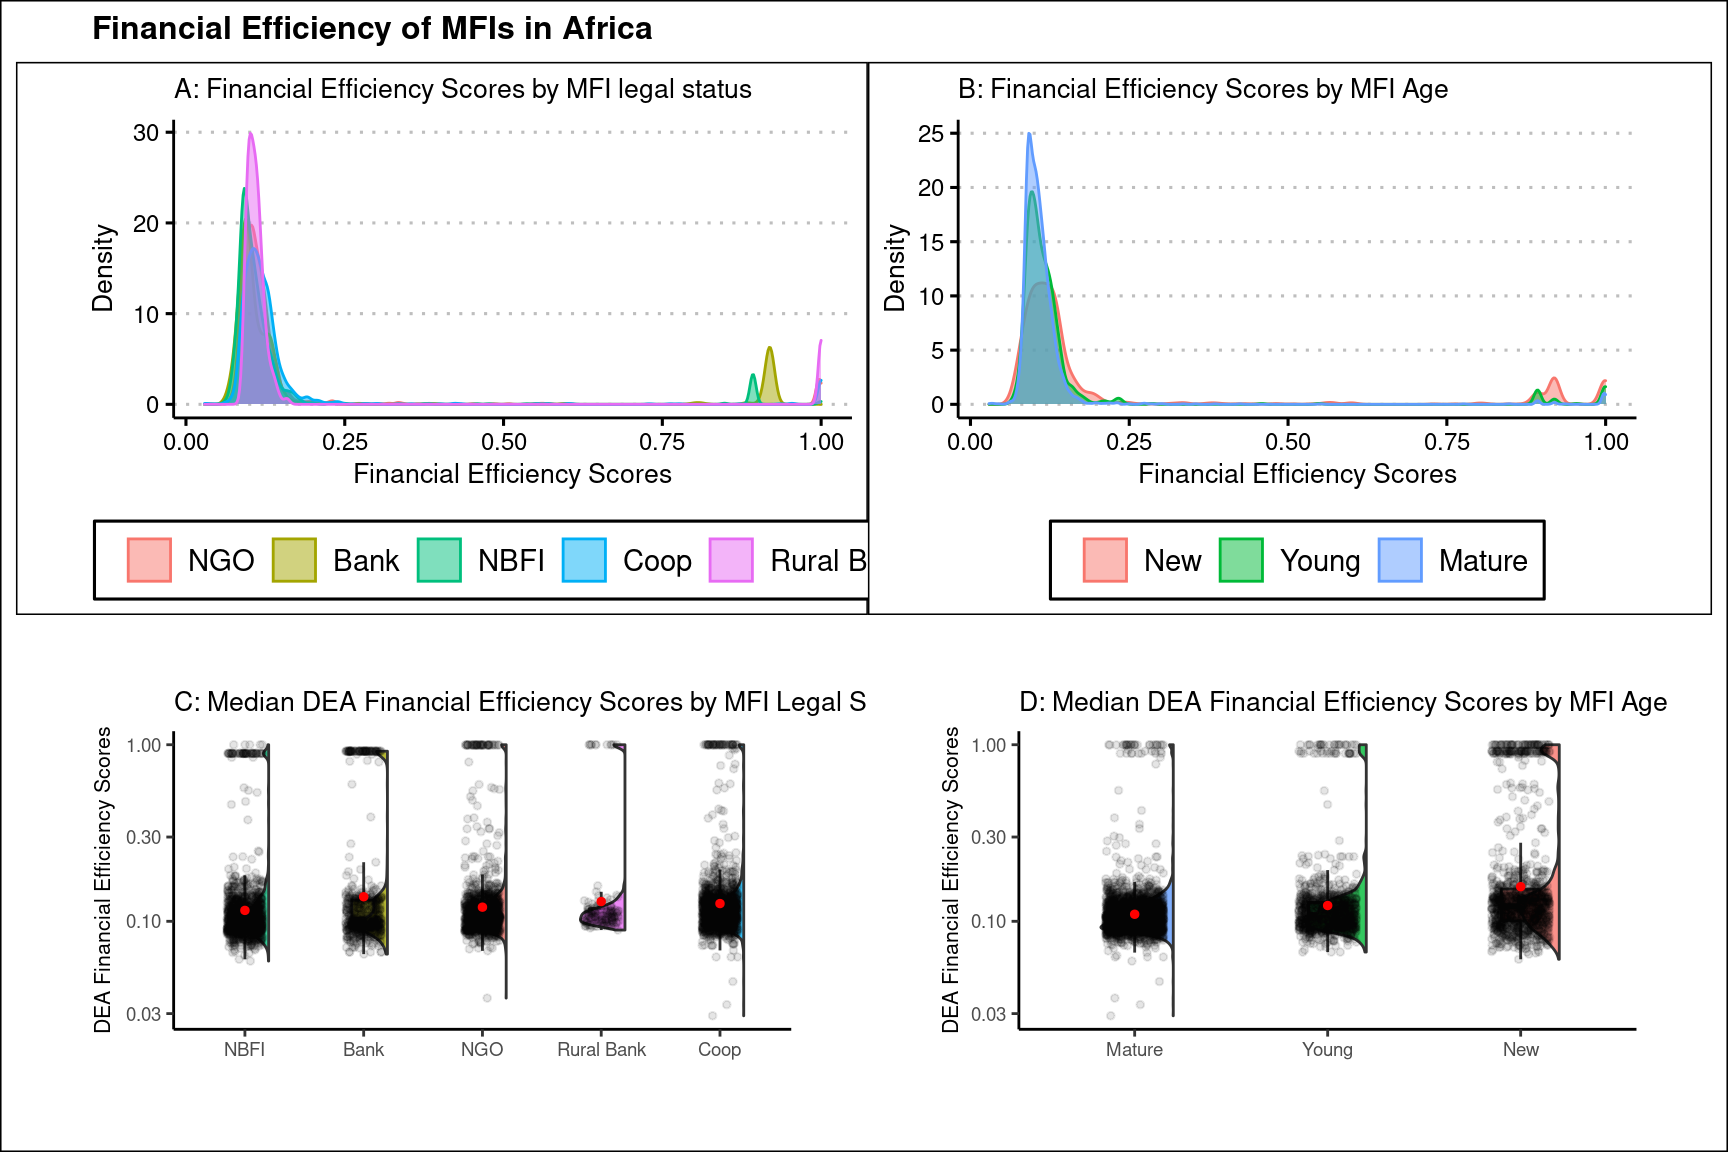
\includegraphics{_main_files/figure-latex/unnamed-chunk-113-1.pdf}
\caption{\label{fig:unnamed-chunk-113}Financial Efficiency Scores for MFIs in Africa}
\end{figure}

\end{landscape}

\newpage

\hypertarget{social-efficiency}{%
\paragraph{Social Efficiency}\label{social-efficiency}}

Overall, the social efficiency of MFIs in Africa is high, with a mean and median of 0.79 and 0.78, respectively. However, as Figures 5.3 and 5.5 show, NGOs have consistently the highest median levels of social efficiency, followed by NBFIs and other forms of MFIs. Rural banks and credit unions, respectively, are the least socially efficient. Considering the financial efficiency scores, it appears that commercialization causes mission drift. Also, both NGOs and NBFIs show a notable decline in social performance over time, which could also be an indictment of the shift towards financial sustainability \autocite{d2017ngos}.

An important observation is that younger MFIs have a higher level of social performance than mature MFIs. Earlier, we saw that younger MFIs also have better financial performance than older MFIs. The implication is that younger MFIs are better at balancing financial and social goals than mature MFIs. The explanation could be that younger MFIs have developed their business model in the face of declining donor support or the complete absence of donor funding and state subsidies. It appears that older MFIs required to shift from the donor and state subsidy reliant model to the commercial model do not perform well. Given that mature MFIs are larger and reach more financially excluded clients, the issue is, therefore, how to support mature MFIs to transition to the financial sustainability model without reducing their outreach.

\begin{landscape}

\begin{figure}
\centering
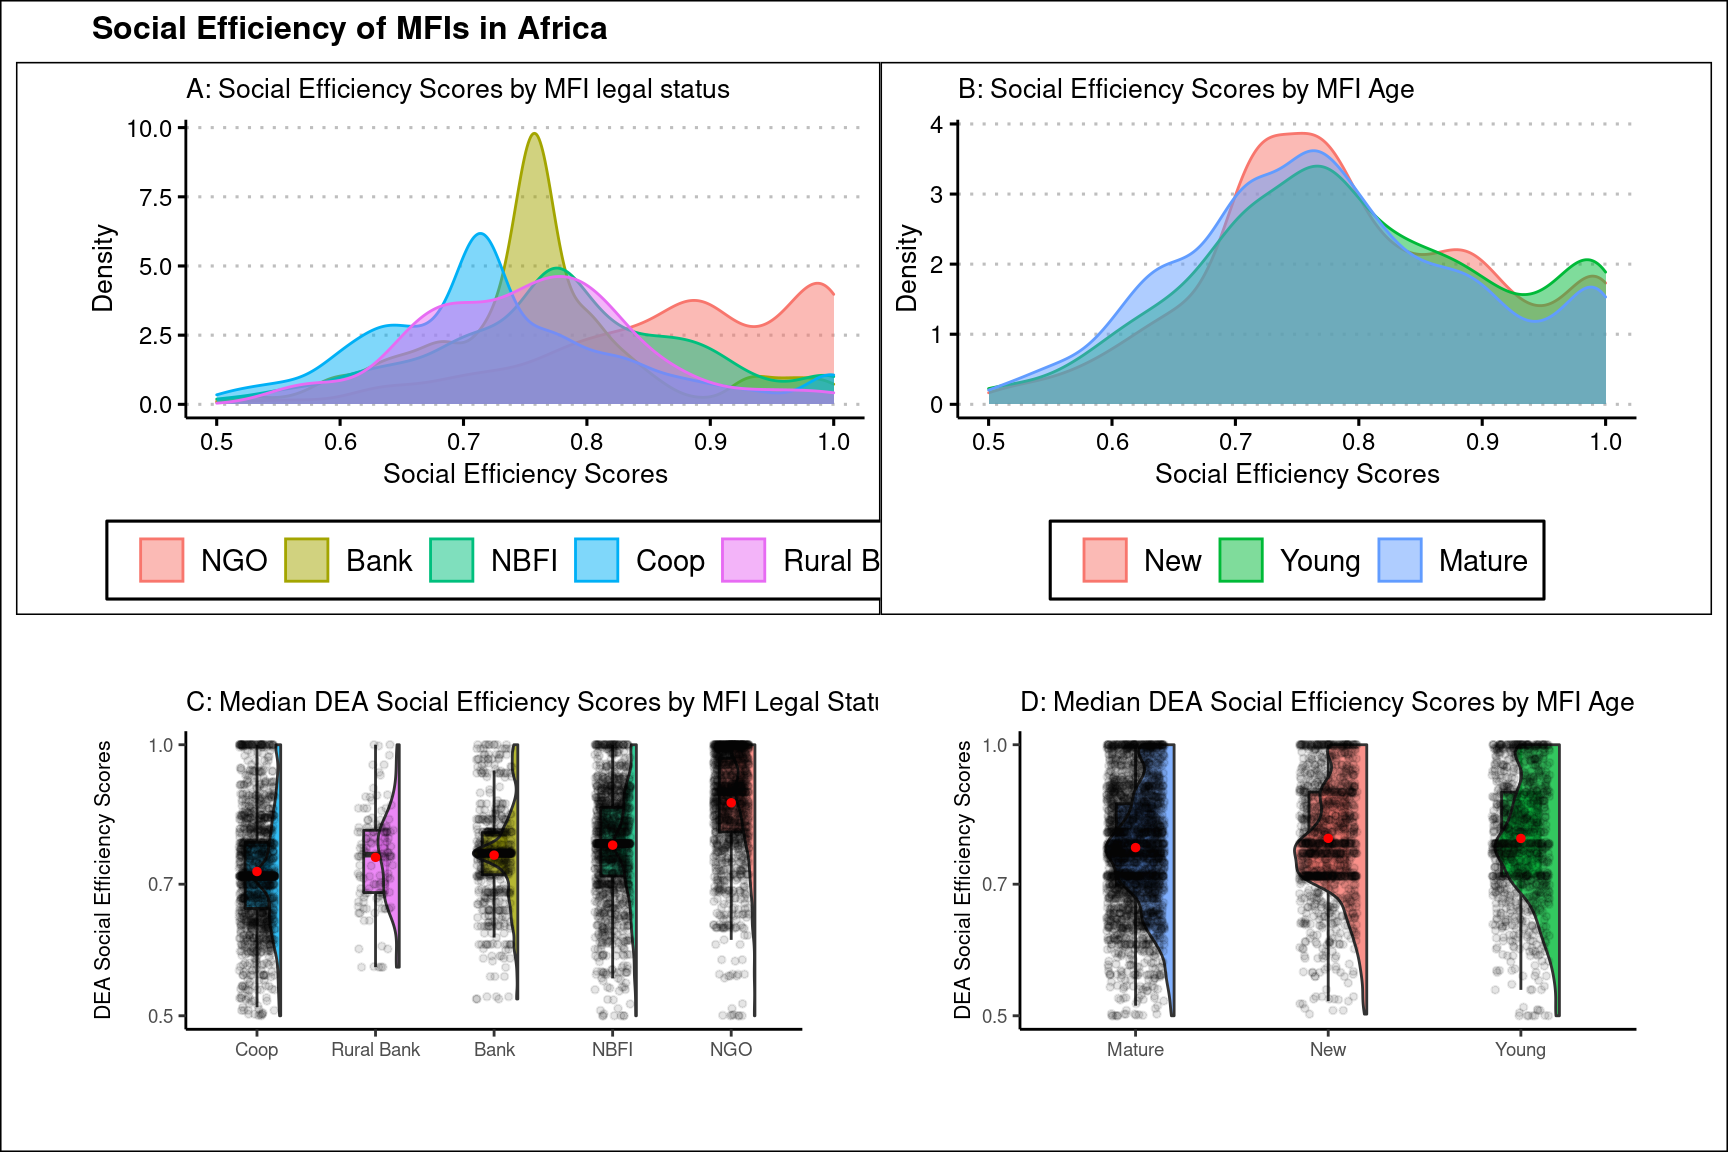
\includegraphics{_main_files/figure-latex/unnamed-chunk-114-1.pdf}
\caption{\label{fig:unnamed-chunk-114}Social Efficiency Scores for MFIs in Africa}
\end{figure}

\end{landscape}

\hypertarget{financial-and-social-socio-financial-efficiency-scores}{%
\paragraph{Financial and Social (Socio-Financial) Efficiency Scores}\label{financial-and-social-socio-financial-efficiency-scores}}

In Figure 5.4, we combine the social and financial metrics. The DEA model now captures the efficiency with which MFIs in Africa convert the inputs (liabilities and equity) into outputs (average loan balance per borrower, percentage of women borrowers, and operational self-sufficiency, OSS). The socio-financial efficiency scores are high, with a median of 0.7947 and a mean of 0.7767. Again, the median socio-financial efficiency metric is highest for NGOs, which is an oddity for we expected commercial firms to dominate if commercialization implies mission expansion (see panels A and C). These results mean that NGOs are better at balancing microfinance's financial and social goals than commercial MFIs. NBFIs, commecial banks, rural banks, and cooperatives follow in that order. These results seem like an indictment of the conversion of MFIs to the commercial model.

In Figure 5.4, panels B and D, we plot the median socio-financial efficiency of MFIs faceted by age. As in the social and financial efficiency analyses, younger MFIs fare better in socio-financial efficiency scores than do older MFIs. Again, these results imply that younger MFIs are better at balancing the social and financial goals of microfinance, as discussed before. Figure 5.4, panel D shows the trends in the socio-financial efficiency of MFIs. While the scores appear stable across time, NGOs score consistently higher. Overall, these results mean that embracing neo-liberalism may be harming social performance without helping improve financial performance.

\begin{landscape}

\newpage

\begin{figure}
\centering
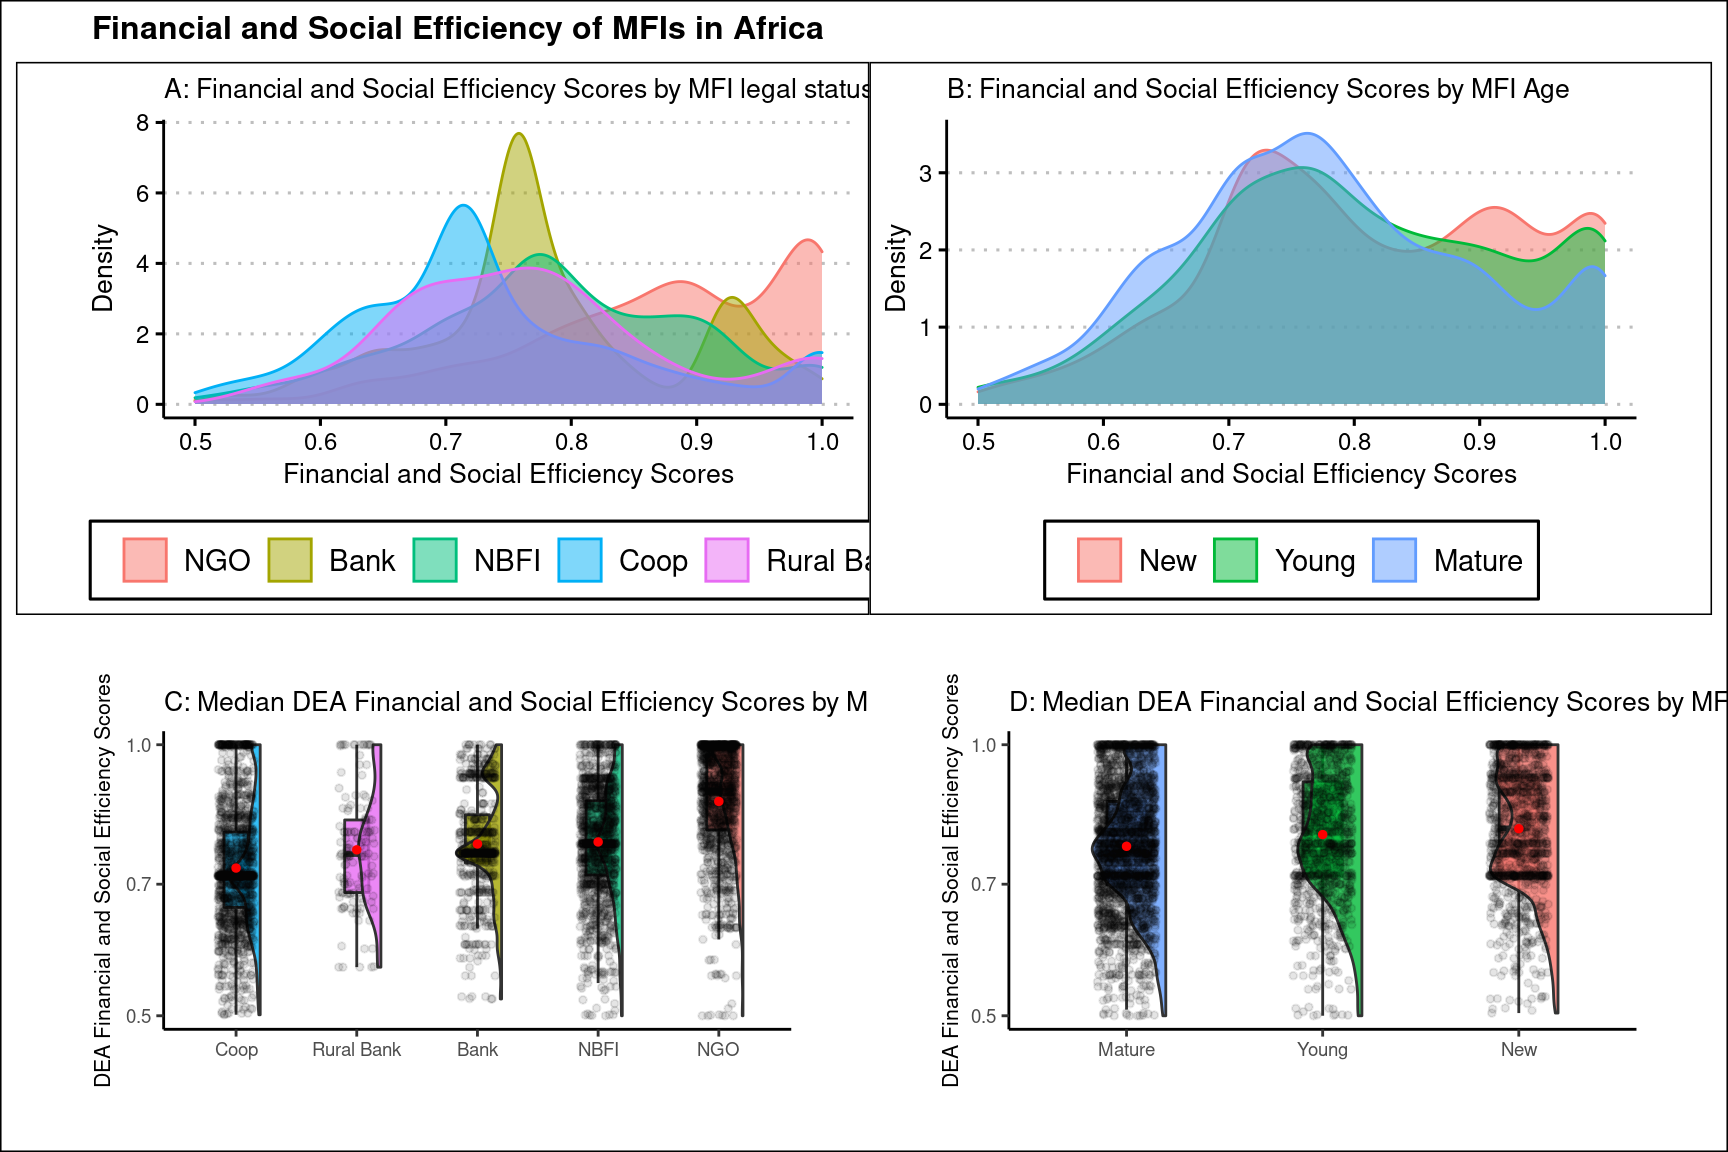
\includegraphics{_main_files/figure-latex/unnamed-chunk-115-1.pdf}
\caption{\label{fig:unnamed-chunk-115}Financial and Social Efficiency Scores for MFIs in Africa}
\end{figure}

\end{landscape}

\newpage

\begin{landscape}

\begin{figure}
\centering
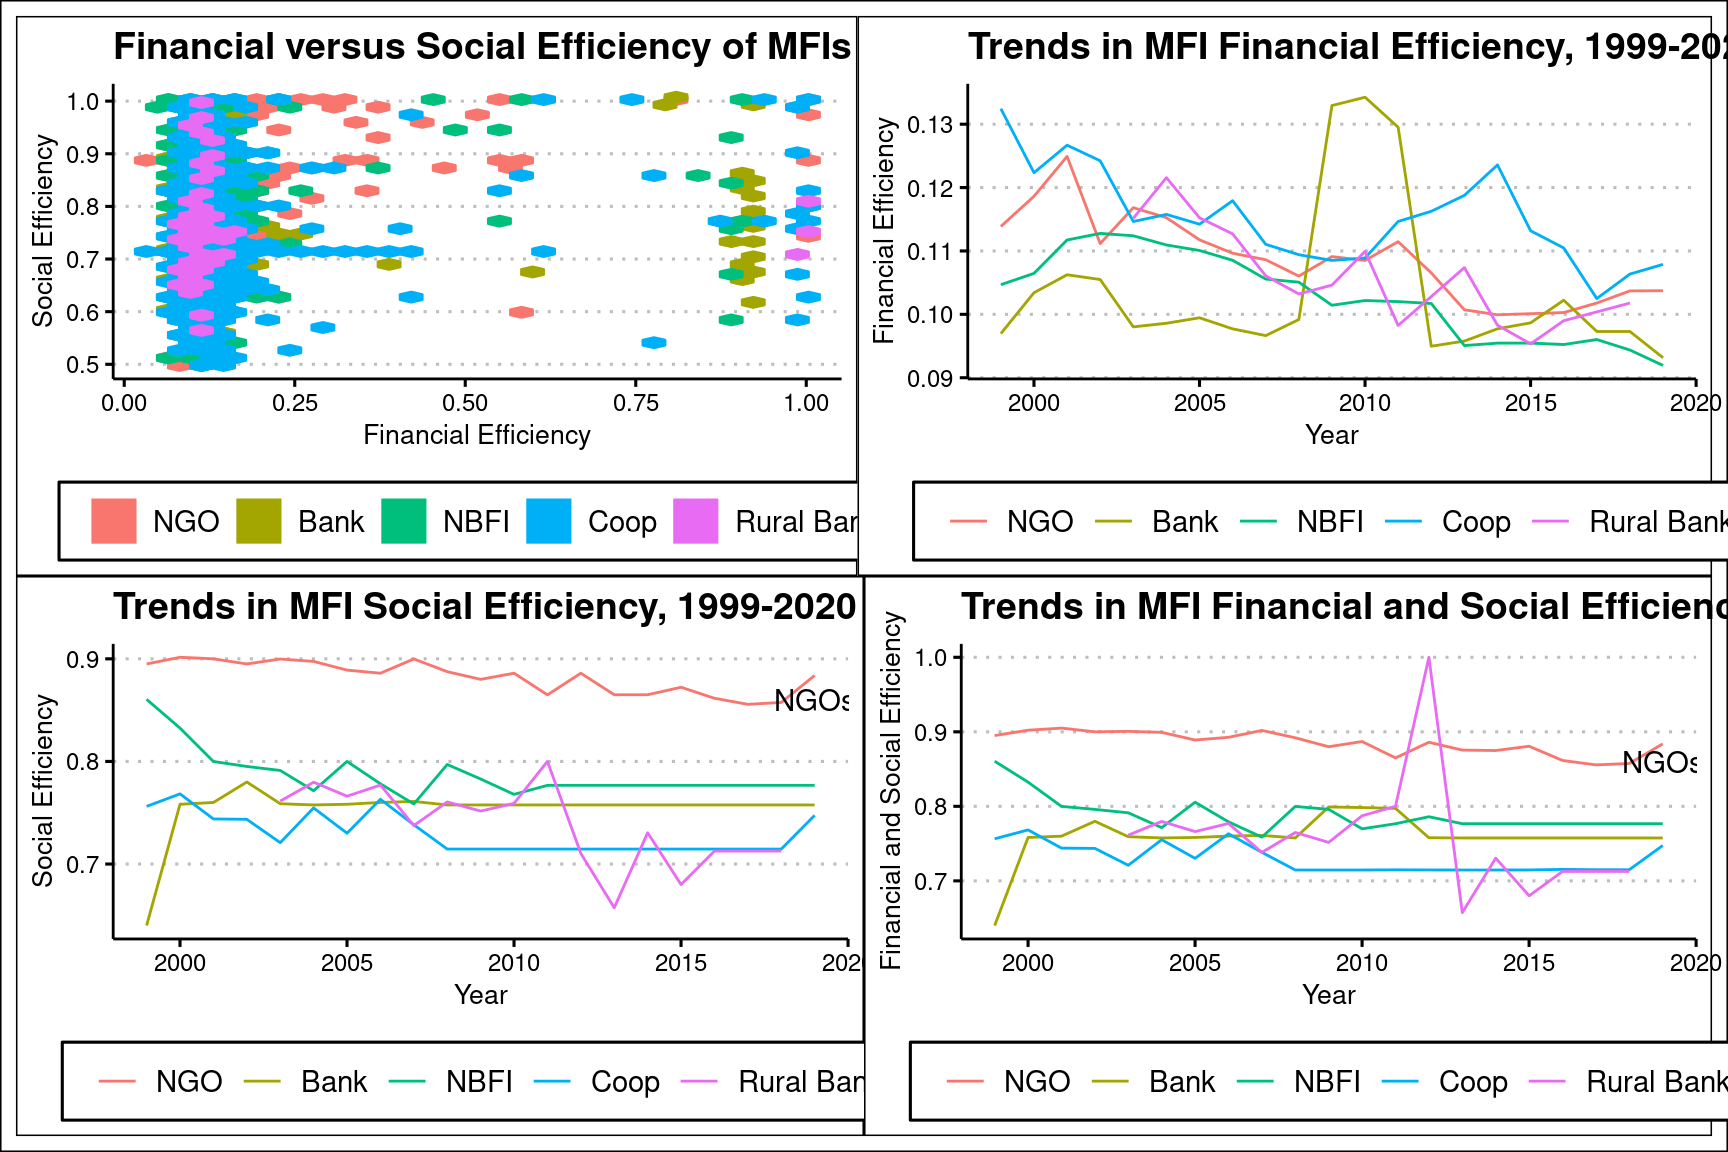
\includegraphics{_main_files/figure-latex/unnamed-chunk-116-1.pdf}
\caption{\label{fig:unnamed-chunk-116}Trends in Financial and Social Efficiency Scores}
\end{figure}

\end{landscape}

\hypertarget{the-independent-variables}{%
\subsection{The Independent Variables}\label{the-independent-variables}}

Table 4.4 shows summary statistics for the independent variables that we employ in the regression models. Profit margin has the highest variability due to a few extreme minimum observations. To proxy the size of an MFI, we take the logarithm of assets. We use all the other independent variables without transformation.

\begin{table}

\caption{\label{tab:unnamed-chunk-117}Summary Statistics: Independent Variables for Regression Model}
\centering
\fontsize{9}{11}\selectfont
\begin{tabular}[t]{lrrrrrrr}
\toprule
Variable & Mean & SD & Min & Q1 & Median & Q3 & Max\\
\midrule
Asset Structure & 0.076 & 0.069 & 0.000 & 0.035 & 0.060 & 0.092 & 0.86\\
KKM & 0.003 & 2.006 & -5.233 & -1.304 & -0.114 & 1.628 & 7.37\\
Private Credit & 2.719 & 0.685 & 0.298 & 2.386 & 2.758 & 3.052 & 6.88\\
Stock Market & 1.141 & 1.473 & 0.000 & 0.000 & 0.000 & 2.428 & 5.80\\
Profit Margin & -7.739 & 513.299 & -35495.625 & -0.181 & 0.048 & 0.189 & 6.20\\
\addlinespace
Assets & 14.946 & 2.262 & 0.693 & 13.540 & 14.858 & 16.416 & 22.98\\
\bottomrule
\multicolumn{8}{l}{\rule{0pt}{1em}Source: Authors construction from the data}\\
\multicolumn{8}{l}{\rule{0pt}{1em}\textit{Note: }}\\
\multicolumn{8}{l}{\rule{0pt}{1em}\textsuperscript{1} Private credit refers to credit advanced by deposit taking banks as a percentage of GDP}\\
\multicolumn{8}{l}{\rule{0pt}{1em}\textsuperscript{2} Stock market is the stock market capitalisation as a percentage of GDP}\\
\end{tabular}
\end{table}

In the next section, we detail the regression output from the drivers of the efficiency of MFIs in Africa.

\hypertarget{regression-analysis-1}{%
\section{Regression Analysis}\label{regression-analysis-1}}

In this section, we regress each of the DEA efficiency scores against the independent variables. We bootstrap the DEA efficiency scores before applying them to the regression model \autocite{simar2000general,tziogkidis2012bootstrap,fethi2010assessing}. Note that the Hausmann Test favours the random effects model (see Appendix 1). However, we also run the fixed effects model for robustness. The purpose of using the bootstrapping approach is two-fold: first, to obtain the bias-corrected estimates and the confidence intervals of DEA-efficiency scores and second, to overcome the correlation problem of DEA-efficiency scores and to provide consistent inferences in explaining the determinants of financial and social efficiency \autocite{assaf2010improving}. The bootstrapped DEA scores serve as the dependent variables in the regression analysis. This section provides results from the regression models on the drivers of the socio-financial efficiency of MFIs in Africa.

\hypertarget{financial-efficiency-of-mfis}{%
\subsection{Financial Efficiency of MFIs}\label{financial-efficiency-of-mfis}}

Table 4.5 shows the results of the regression analysis with financial efficiency as the dependent variable. The significant drivers of financial efficiency are asset structure, MFI size proxied by the logarithm of total assets, and stock market capitalisation to GDP. Current legal status has a weak relationship with financial efficiency. The regression analysis shows that commercial banks and rural banks have significantly better financial efficiency, which goes against the visualisation in Figure 5.2. The extreme values in the financial performance of banks and rural banks could explain this contradiction. Considering this, NGOs do better financially than all the legal forms of MFIs except cooperatives.

These results go against the stated objectives of MFI commercialisation. The commercial model of microfinance aims at increasing the financial sustainability of MFIs, which would allow for their sustainability without reliance on donations and subsidies \autocite{d2017ngos}. Again, financial sustainability by MFIs would lead to mission expansion by using profits to reach the financially excluded. However, the data shows that this is not the case. Overall, the financial performance of MFIs is poor \autocite{mersland2010microfinance}. Also, the commercial MFIs do not outperform NGOs in financial performance in the sample dataset. It then seems like commercialisation does not necessarily translate into financial sustainability. And given the relatively good financial performance by NGOs that do not explicitly prioritise profitability, it appears that the win-win school has the upper hand. MFIs can balance financial and social goals while retaining the NGO model that focuses on social goals.

The asset structure of MFIs has an inverse relationship with financial efficiency. As noted earlier, asset structure or asset tangibility is the ratio of non-current assets to total assets of an MFI. The results then imply that investment in physical infrastructure harms financial sustainability \autocite{iman2018mobile,demirguc2018global}. The results are consistent with the empirical literature in microfinance because serving the financially excluded is expensive and may not yield economies of scale to offset the investment in physical infrastructure by MFIs \autocite{quayes2019probability}. The advent of Fintech allows MFIs to reach out to the financially excluded without high expenditures in brick and mortar branches and other physical assets \autocite{iman2018mobile}. However, given that most financially excluded people also suffer from financial illiteracy, MFIs still must deploy field workers or mobile banking units in targeted areas \autocite{allen2014african}. Hence, there is an opportunity for research into how Fintech affects the investment in physical infrastructure, profitability and outreach of MFIs in Africa.

The size of an MFI is also negatively related to the financial efficiency of MFIs in Africa. Large, older MFIs have lower financial efficiency scores relative to smaller, younger ones, which could arise due to dis-economies of scale. Also, larger, older MFIs may not emphasise financial sustainability, given they receive relatively more donations. If donors emphasise outreach vis-a-vis financial sustainability, this could explain the lower levels of financial performance by older MFIs \autocite{d2013unsubsidized}. The ratio of stock market capitalisation to GDP has a weak positive relationship with financial efficiency, implying that MFIs operating in countries with better functioning capital markets exhibit better financial performance. Lower incidence of financial exclusion in countries with well developed capital markets could explain the relationship \autocite{allen2014african}. The ratio of private credit to GDP is insignificant. The remaining variables, age and institutional quality, have no significant relationship with financial efficiency. However, as we saw earlier in Table 4.2, younger MFIs have marginally higher financial performance, which is not important in the regression.

\newpage

\begin{landscape}

\begin{table}[!htbp] \centering 
  \caption{Regression Output for Financial Efficiency (Standard Errors in Brackets)} 
  \label{} 
\tiny 
\begin{tabular}{@{\extracolsep{5pt}}lD{.}{.}{-3} D{.}{.}{-3} D{.}{.}{-3} D{.}{.}{-3} D{.}{.}{-3} D{.}{.}{-3} } 
\\[-1.8ex]\hline 
\hline \\[-1.8ex] 
 & \multicolumn{6}{c}{\textit{Dependent variable:}} \\ 
\cline{2-7} 
\\[-1.8ex] & \multicolumn{6}{c}{DEA Efficiency Score} \\ 
\\[-1.8ex] & \multicolumn{1}{c}{(1)} & \multicolumn{1}{c}{(2)} & \multicolumn{1}{c}{(3)} & \multicolumn{1}{c}{(4)} & \multicolumn{1}{c}{(5)} & \multicolumn{1}{c}{(6)}\\ 
\hline \\[-1.8ex] 
 currentlegalstatusBank &  &  &  & 0.127^{***} & 0.012 & 0.028^{**} \\ 
  &  &  &  & (0.025) & (0.020) & (0.013) \\ 
  & & & & & & \\ 
 currentlegalstatusNBFI &  &  &  & 0.019 & -0.006 & 0.005 \\ 
  &  &  &  & (0.019) & (0.015) & (0.009) \\ 
  & & & & & & \\ 
 currentlegalstatusCoop & -0.002 & -0.001 & -0.0004 & -0.003 & -0.005 & 0.008 \\ 
  & (0.019) & (0.018) & (0.022) & (0.015) & (0.014) & (0.009) \\ 
  & & & & & & \\ 
 currentlegalstatusRural Bank &  &  &  & 0.053^{*} & -0.038 & -0.004 \\ 
  &  &  &  & (0.031) & (0.028) & (0.028) \\ 
  & & & & & & \\ 
 ageYoung & 0.002 & 0.001 & 0.002 & 0.001 & 0.001 & 0.002 \\ 
  & (0.002) & (0.002) & (0.002) & (0.003) & (0.003) & (0.002) \\ 
  & & & & & & \\ 
 ageMature & 0.005^{*} & 0.004 & 0.005 & 0.002 & 0.003 & 0.004 \\ 
  & (0.003) & (0.003) & (0.003) & (0.003) & (0.003) & (0.003) \\ 
  & & & & & & \\ 
 kkm & -0.002 & -0.002^{*} & -0.002 & -0.0001 & -0.001 & 0.0004 \\ 
  & (0.001) & (0.001) & (0.001) & (0.001) & (0.001) & (0.001) \\ 
  & & & & & & \\ 
 asset\_structure & -0.070^{***} & -0.060^{***} & -0.066^{***} & -0.087^{***} & -0.069^{***} & -0.067^{***} \\ 
  & (0.015) & (0.016) & (0.016) & (0.018) & (0.017) & (0.016) \\ 
  & & & & & & \\ 
 pcrdbgdp & -0.001 & 0.002 & 0.002 & -0.002 & -0.003 & -0.004 \\ 
  & (0.003) & (0.003) & (0.003) & (0.004) & (0.004) & (0.003) \\ 
  & & & & & & \\ 
 stmktcap & 0.004^{*} & 0.004 & 0.007^{***} & 0.005^{**} & 0.003 & 0.005^{***} \\ 
  & (0.002) & (0.002) & (0.002) & (0.003) & (0.002) & (0.002) \\ 
  & & & & & & \\ 
 log(assets) & -0.159^{***} & -0.138^{***} & -0.128^{***} & -0.183^{***} & -0.152^{***} & -0.127^{***} \\ 
  & (0.012) & (0.012) & (0.017) & (0.013) & (0.013) & (0.016) \\ 
  & & & & & & \\ 
\hline \\[-1.8ex] 
Model & Within & Within & Within & Random & Random & Random \\ 
Data & Full & 3 Years and over & 5 Years and over & Full & 3 Years and over & 5 Years and over \\ 
Observations & \multicolumn{1}{c}{4,782} & \multicolumn{1}{c}{3,840} & \multicolumn{1}{c}{3,165} & \multicolumn{1}{c}{4,782} & \multicolumn{1}{c}{3,840} & \multicolumn{1}{c}{3,165} \\ 
R$^{2}$ & \multicolumn{1}{c}{0.078} & \multicolumn{1}{c}{0.073} & \multicolumn{1}{c}{0.098} & \multicolumn{1}{c}{0.151} & \multicolumn{1}{c}{0.095} & \multicolumn{1}{c}{0.101} \\ 
Adjusted R$^{2}$ & \multicolumn{1}{c}{-0.142} & \multicolumn{1}{c}{-0.057} & \multicolumn{1}{c}{-0.003} & \multicolumn{1}{c}{0.146} & \multicolumn{1}{c}{0.088} & \multicolumn{1}{c}{0.093} \\ 
F Statistic & \multicolumn{1}{c}{11.600$^{***}$ (df = 28; 3862)} & \multicolumn{1}{c}{9.520$^{***}$ (df = 28; 3366)} & \multicolumn{1}{c}{11.100$^{***}$ (df = 28; 2845)} & \multicolumn{1}{c}{380.000$^{***}$} & \multicolumn{1}{c}{281.000$^{***}$} & \multicolumn{1}{c}{293.000$^{***}$} \\ 
\hline 
\hline \\[-1.8ex] 
\textit{Note:}  & \multicolumn{6}{r}{$^{*}$p$<$0.1; $^{**}$p$<$0.05; $^{***}$p$<$0.01} \\ 
\end{tabular} 
\end{table}

\end{landscape}

\newpage

\hypertarget{drivers-of-social-efficiency-of-mfis}{%
\subsection{Drivers of Social Efficiency of MFIs}\label{drivers-of-social-efficiency-of-mfis}}

Unlike financial performance, the legal form of an MFI is the dominant driver of social performance (see Table 4.6). Consistent with Figure 5.3, NGOs have significantly higher social performance levels than all the other legal forms of MFI. The concern by the welfare school of microfinance is that the levels of outreach by NGOs to the financially excluded could be affected by focusing on financial sustainability. However, as the previous section shows, NGOs do not fare badly in financial efficiency than other legal forms of MFI. It means, therefore, that NGOs could aim at a degree of financial efficiency while still maintaining their social goals. As \textcite{mersland2019social} note, the mission statements of MFIs have a significant relationship with the performance of these MFIs. Given that NGOs have the stated mission of reaching the unbanked, they are better positioned to achieve these social goals. If NGOs are to give financial goals as much weight as social goals, there is likely to be a trade-off, more so where fund providers put pressure on management to make financial returns.

The results are consistent with the data visualisations. Credit unions have the objective of serving subscribed members within a designated geographic location or a common professional background. It is not their mission to explicitly target social performance \autocite{mathuva2017achieving}. The contestation here is between NGOs and the other commercial entities, excluding credit unions. The results illustrate that MFIs that exclusively target social performance tend to achieve more socially. Hence the place of the social mission of an MFI is central to achieving social objectives, a view that is in line with findings by \textcite{berbegal2019impact}.

Both stock markets capitalisation to GDP and private credit to GDP have a negative and significant relationship with social performance. These two metrics capture the levels of capital market development. People in countries with higher levels of financial development have lower incidences of financial exclusion, on average, relative to people in countries with lower levels of financial inclusion. This observation is despite the concurrence in the literature that the ability to access financial services does not necessarily translate into the usage of financial services. However, access to financial services is a necessary precondition for people to use financial services \autocite{allen2013resolving,jarotschkin2013microfinance}. Financial development means better financial infrastructure that allows people who could otherwise not use financial services because of lack of access to these services.

Institutional quality (KKM) has a mixed but insignificant relationship with the social performance of MFIs. As expected, asset structure has a positive, albeit negligible connection with social performance, given that MFIs that have a more significant presence in financially under-served communities would tend to serve more financially excluded clients. Likewise, the size of an MFI shows a positive but insignificant relationship with social outreach. Again, consistent with the data visualisation, younger MFIs have better levels of social performance than older MFIs, although the coefficients are not significant in the regression. The result seems odd because younger MFIs started when the sustainability school was gaining ground, meaning low donations and subsidies \autocite{d2013unsubsidized}. But given that younger MFIs are smaller, they may serve geographically limited areas to reach more financially excluded clients. The broader coverage by older MFIs makes it hard for them to focus on social goals, given the financial implications of sustaining their presence in these settings.

\hypertarget{socio-financial-efficiency-of-mfis}{%
\subsection{Socio-Financial Efficiency of MFIs}\label{socio-financial-efficiency-of-mfis}}

In this regression model, we examine joint social and financial efficiency (socio-financial efficiency) drivers. Specifically, we seek to uncover how well MFIs convert their inputs into financial (operational self-sufficiency) and social goals (percentage of female borrowers and average loan balance per borrower). The results in Table 4.7 show that, like social efficiency, the statistically significant drivers of socio-financial efficiency are legal status and the ratio of stock market capitalisation to GDP. Specifically, the regression analysis shows that NGOs have higher socio-financial efficiency scores than the other legal forms of MFIs, confirming the results of the exploratory data analysis. These results suggest that transformed MFIs do not achieve the attained benefits of commercialisation, that is, increased financial sustainability, which allows for greater outreach to the financially excluded (mission expansion) \autocite{mersland2010microfinance}. Instead, it is NGOs that are capable of balancing financial and social goals. Like in social pursuits, socio-financial efficiency has a negative relationship with stock market capitalisation to GDP, highlighting the importance of financial sector development in enabling financial inclusion \autocite{allen2013resolving}.

\begin{landscape}

\newpage

\begin{table}[!htbp] \centering 
  \caption{Regression Output for Social Efficiency (Standard Errors in Brackets)} 
  \label{} 
\tiny 
\begin{tabular}{@{\extracolsep{5pt}}lD{.}{.}{-3} D{.}{.}{-3} D{.}{.}{-3} D{.}{.}{-3} D{.}{.}{-3} D{.}{.}{-3} } 
\\[-1.8ex]\hline 
\hline \\[-1.8ex] 
 & \multicolumn{6}{c}{\textit{Dependent variable:}} \\ 
\cline{2-7} 
\\[-1.8ex] & \multicolumn{6}{c}{DEA Efficiency Scores} \\ 
\\[-1.8ex] & \multicolumn{1}{c}{(1)} & \multicolumn{1}{c}{(2)} & \multicolumn{1}{c}{(3)} & \multicolumn{1}{c}{(4)} & \multicolumn{1}{c}{(5)} & \multicolumn{1}{c}{(6)}\\ 
\hline \\[-1.8ex] 
 currentlegalstatusBank &  &  &  & -0.106^{***} & -0.096^{***} & -0.095^{***} \\ 
  &  &  &  & (0.014) & (0.020) & (0.022) \\ 
  & & & & & & \\ 
 currentlegalstatusNBFI &  &  &  & -0.084^{***} & -0.080^{***} & -0.077^{***} \\ 
  &  &  &  & (0.011) & (0.014) & (0.015) \\ 
  & & & & & & \\ 
 currentlegalstatusCoop & 0.047 & 0.048 & 0.048 & -0.137^{***} & -0.122^{***} & -0.124^{***} \\ 
  & (0.054) & (0.057) & (0.063) & (0.010) & (0.014) & (0.017) \\ 
  & & & & & & \\ 
 currentlegalstatusRural Bank &  &  &  & -0.103^{***} & -0.124^{***} & -0.130^{**} \\ 
  &  &  &  & (0.022) & (0.033) & (0.052) \\ 
  & & & & & & \\ 
 ageYoung & -0.001 & -0.003 & -0.001 & -0.002 & -0.003 & -0.001 \\ 
  & (0.005) & (0.005) & (0.006) & (0.004) & (0.005) & (0.006) \\ 
  & & & & & & \\ 
 ageMature & -0.004 & -0.005 & -0.002 & -0.006 & -0.008 & -0.003 \\ 
  & (0.007) & (0.008) & (0.009) & (0.006) & (0.007) & (0.009) \\ 
  & & & & & & \\ 
 kkm & 0.0004 & 0.0003 & -0.0002 & -0.001 & -0.003 & -0.003 \\ 
  & (0.003) & (0.003) & (0.004) & (0.002) & (0.002) & (0.003) \\ 
  & & & & & & \\ 
 asset\_structure & 0.024 & 0.029 & 0.036 & 0.010 & 0.022 & 0.029 \\ 
  & (0.029) & (0.034) & (0.042) & (0.027) & (0.032) & (0.040) \\ 
  & & & & & & \\ 
 pcrdbgdp & -0.011 & -0.013 & -0.013 & -0.009^{*} & -0.011^{*} & -0.010 \\ 
  & (0.007) & (0.008) & (0.009) & (0.005) & (0.007) & (0.007) \\ 
  & & & & & & \\ 
 stmktcap & -0.013^{***} & -0.014^{***} & -0.012^{**} & -0.002 & -0.002 & -0.004 \\ 
  & (0.004) & (0.004) & (0.005) & (0.003) & (0.003) & (0.004) \\ 
  & & & & & & \\ 
 log(assets) & 0.026 & 0.035 & 0.034 & -0.029 & -0.014 & -0.006 \\ 
  & (0.026) & (0.028) & (0.045) & (0.018) & (0.025) & (0.039) \\ 
  & & & & & & \\ 
\hline \\[-1.8ex] 
Model & Within & Within & Within & Random & Random & Random \\ 
Data & Full & 3 Years and over & 5 Years and over & Full & 3 Years and over & 5 Years and over \\ 
Observations & \multicolumn{1}{c}{4,782} & \multicolumn{1}{c}{3,840} & \multicolumn{1}{c}{3,165} & \multicolumn{1}{c}{4,782} & \multicolumn{1}{c}{3,840} & \multicolumn{1}{c}{3,165} \\ 
R$^{2}$ & \multicolumn{1}{c}{0.037} & \multicolumn{1}{c}{0.039} & \multicolumn{1}{c}{0.038} & \multicolumn{1}{c}{0.619} & \multicolumn{1}{c}{0.348} & \multicolumn{1}{c}{0.200} \\ 
Adjusted R$^{2}$ & \multicolumn{1}{c}{-0.192} & \multicolumn{1}{c}{-0.096} & \multicolumn{1}{c}{-0.070} & \multicolumn{1}{c}{0.617} & \multicolumn{1}{c}{0.342} & \multicolumn{1}{c}{0.192} \\ 
F Statistic & \multicolumn{1}{c}{5.290$^{***}$ (df = 28; 3862)} & \multicolumn{1}{c}{4.840$^{***}$ (df = 28; 3366)} & \multicolumn{1}{c}{3.970$^{***}$ (df = 28; 2845)} & \multicolumn{1}{c}{422.000$^{***}$} & \multicolumn{1}{c}{244.000$^{***}$} & \multicolumn{1}{c}{184.000$^{***}$} \\ 
\hline 
\hline \\[-1.8ex] 
\textit{Note:}  & \multicolumn{6}{r}{$^{*}$p$<$0.1; $^{**}$p$<$0.05; $^{***}$p$<$0.01} \\ 
\end{tabular} 
\end{table}

\end{landscape}

\begin{landscape}

\newpage

\begin{table}[!htbp] \centering 
  \caption{Regression Output for Joint Financial and Social Efficiency (Standard Errors in Brackets)} 
  \label{} 
\tiny 
\begin{tabular}{@{\extracolsep{5pt}}lD{.}{.}{-3} D{.}{.}{-3} D{.}{.}{-3} D{.}{.}{-3} D{.}{.}{-3} D{.}{.}{-3} } 
\\[-1.8ex]\hline 
\hline \\[-1.8ex] 
 & \multicolumn{6}{c}{\textit{Dependent variable:}} \\ 
\cline{2-7} 
\\[-1.8ex] & \multicolumn{6}{c}{depvar} \\ 
\\[-1.8ex] & \multicolumn{1}{c}{(1)} & \multicolumn{1}{c}{(2)} & \multicolumn{1}{c}{(3)} & \multicolumn{1}{c}{(4)} & \multicolumn{1}{c}{(5)} & \multicolumn{1}{c}{(6)}\\ 
\hline \\[-1.8ex] 
 currentlegalstatusBank &  &  &  & -0.106^{***} & -0.096^{***} & -0.095^{***} \\ 
  &  &  &  & (0.015) & (0.020) & (0.022) \\ 
  & & & & & & \\ 
 currentlegalstatusNBFI &  &  &  & -0.084^{***} & -0.080^{***} & -0.077^{***} \\ 
  &  &  &  & (0.012) & (0.014) & (0.015) \\ 
  & & & & & & \\ 
 currentlegalstatusCoop & 0.047 & 0.048 & 0.048 & -0.137^{***} & -0.122^{***} & -0.124^{***} \\ 
  & (0.055) & (0.058) & (0.063) & (0.011) & (0.014) & (0.017) \\ 
  & & & & & & \\ 
 currentlegalstatusRural Bank &  &  &  & -0.103^{***} & -0.124^{***} & -0.130^{**} \\ 
  &  &  &  & (0.023) & (0.033) & (0.052) \\ 
  & & & & & & \\ 
 ageYoung & -0.001 & -0.003 & -0.001 & -0.002 & -0.003 & -0.001 \\ 
  & (0.005) & (0.005) & (0.006) & (0.004) & (0.005) & (0.006) \\ 
  & & & & & & \\ 
 ageMature & -0.004 & -0.005 & -0.002 & -0.006 & -0.008 & -0.003 \\ 
  & (0.007) & (0.008) & (0.009) & (0.006) & (0.008) & (0.009) \\ 
  & & & & & & \\ 
 kkm & 0.0004 & 0.0003 & -0.0002 & -0.001 & -0.003 & -0.003 \\ 
  & (0.003) & (0.003) & (0.004) & (0.002) & (0.002) & (0.003) \\ 
  & & & & & & \\ 
 asset\_structure & 0.024 & 0.029 & 0.036 & 0.010 & 0.022 & 0.029 \\ 
  & (0.029) & (0.034) & (0.042) & (0.028) & (0.033) & (0.040) \\ 
  & & & & & & \\ 
 pcrdbgdp & -0.011 & -0.013 & -0.013 & -0.009^{*} & -0.011^{*} & -0.010 \\ 
  & (0.007) & (0.008) & (0.009) & (0.006) & (0.007) & (0.007) \\ 
  & & & & & & \\ 
 stmktcap & -0.013^{***} & -0.014^{***} & -0.012^{**} & -0.002 & -0.002 & -0.004 \\ 
  & (0.004) & (0.004) & (0.005) & (0.003) & (0.003) & (0.004) \\ 
  & & & & & & \\ 
 log(assets) & 0.026 & 0.035 & 0.034 & -0.029 & -0.014 & -0.006 \\ 
  & (0.026) & (0.028) & (0.045) & (0.019) & (0.025) & (0.039) \\ 
  & & & & & & \\ 
\hline \\[-1.8ex] 
Model & Within & Within & Within & Random & Random & Random \\ 
Data & Full & 3 Years and over & 5 Years and over & Full & 3 Years and over & 5 Years and over \\ 
Observations & \multicolumn{1}{c}{4,782} & \multicolumn{1}{c}{3,840} & \multicolumn{1}{c}{3,165} & \multicolumn{1}{c}{4,782} & \multicolumn{1}{c}{3,840} & \multicolumn{1}{c}{3,165} \\ 
R$^{2}$ & \multicolumn{1}{c}{0.037} & \multicolumn{1}{c}{0.039} & \multicolumn{1}{c}{0.038} & \multicolumn{1}{c}{0.619} & \multicolumn{1}{c}{0.348} & \multicolumn{1}{c}{0.200} \\ 
Adjusted R$^{2}$ & \multicolumn{1}{c}{-0.192} & \multicolumn{1}{c}{-0.096} & \multicolumn{1}{c}{-0.070} & \multicolumn{1}{c}{0.617} & \multicolumn{1}{c}{0.342} & \multicolumn{1}{c}{0.192} \\ 
F Statistic & \multicolumn{1}{c}{5.290$^{***}$ (df = 28; 3862)} & \multicolumn{1}{c}{4.840$^{***}$ (df = 28; 3366)} & \multicolumn{1}{c}{3.970$^{***}$ (df = 28; 2845)} & \multicolumn{1}{c}{422.000$^{***}$} & \multicolumn{1}{c}{244.000$^{***}$} & \multicolumn{1}{c}{184.000$^{***}$} \\ 
\hline 
\hline \\[-1.8ex] 
\textit{Note:}  & \multicolumn{6}{r}{$^{*}$p$<$0.1; $^{**}$p$<$0.05; $^{***}$p$<$0.01} \\ 
\end{tabular} 
\end{table}

\end{landscape}

\newpage

\hypertarget{robustness-tests}{%
\subsection{Robustness Tests}\label{robustness-tests}}

We first run the fixed and random effects models for the entire dataset for robustness, with the results reported in Tables 5.5, 5.6 and 5.7. Secondly, we check for outliers by winsorising the data. To do this, we drop the top 10\% and bottom 10\% observations of the independent variables and rerun the fixed and random effects regressions. The results are in Appendix 3 (Table 4.9). The results correspond to those in Tables 5.5 to 5.7 except for the magnitude of the regression coefficients.

Given the panel structure of data, there is a possibility of cross-sectional dependence and serial correlation. We correct the standard errors -- presenting the panel corrected standard errors to deal with these problems. Appendix 4-6 contain plots examining the normality of residuals for the regression outputs in Table 4.5. The results show slight deviations from normality, which may not be an issue given the large sample size.

\hypertarget{conclusion-2}{%
\section{Conclusion}\label{conclusion-2}}

This study examined the levels and drivers of financial efficiency, social efficiency, and socio-financial efficiency of MFIs in Africa, particularly along MFI legal status lines. NGOs have the highest levels of social efficiency and socio-financial efficiency, whereas cooperatives have the least. Cooperatives, rural banks, and NGOs, in that order, have the best financial performance scores, while NBFIs trail. MFI legal status and the level of capital markets development proxied by stock market capitalisation to GDP and private credit to GDP are the critical drivers of social efficiency and socio-financial efficiency. MFI legal status, asset structure, size, and the country-level financial development proxy of stock market capitalisation to GDP are the significant factors in the case of financial efficiency. These results suggest the possibility of mission drift where MFIs that focus primarily on making financial returns perform relatively poorly in outreach to the financially excluded. NGOs appear better at balancing financial returns and social goals, even when not mainly targeting profitability or financial sustainability. Given that the legitimacy of MFIs rests on how well they balance returns and social goals, it appears that commercialisation is not working well as the researchers subscribing to the financial sustainability view of microfinance have predicted.

\newpage

\hypertarget{appendices-2}{%
\section{Appendices}\label{appendices-2}}

\hypertarget{appendix-1-hausmann-test-fixed-vs-random-effects}{%
\subsection{Appendix 1: Hausmann Test; Fixed vs Random effects}\label{appendix-1-hausmann-test-fixed-vs-random-effects}}

\begin{table}[!h]

\caption{\label{tab:unnamed-chunk-128}Results of the Hausmann Tests}
\centering
\fontsize{9}{11}\selectfont
\begin{tabu} to \linewidth {>{\raggedleft}X>{\raggedleft}X>{\raggedleft}X>{\raggedright}X>{\raggedright}X}
\toprule
Statistic & P.value & Parameter & Method & Alternative\\
\midrule
73.4 & 0 & 8 & Hausman Test & one model is inconsistent\\
62.5 & 0 & 8 & Hausman Test & one model is inconsistent\\
84.6 & 0 & 8 & Hausman Test & one model is inconsistent\\
\bottomrule
\end{tabu}
\end{table}

\begin{landscape}

\hypertarget{appendix-2-visualization-of-dea-inputs-and-outputs}{%
\subsection{Appendix 2: Visualization of DEA Inputs and Outputs}\label{appendix-2-visualization-of-dea-inputs-and-outputs}}

\begin{figure}
\centering
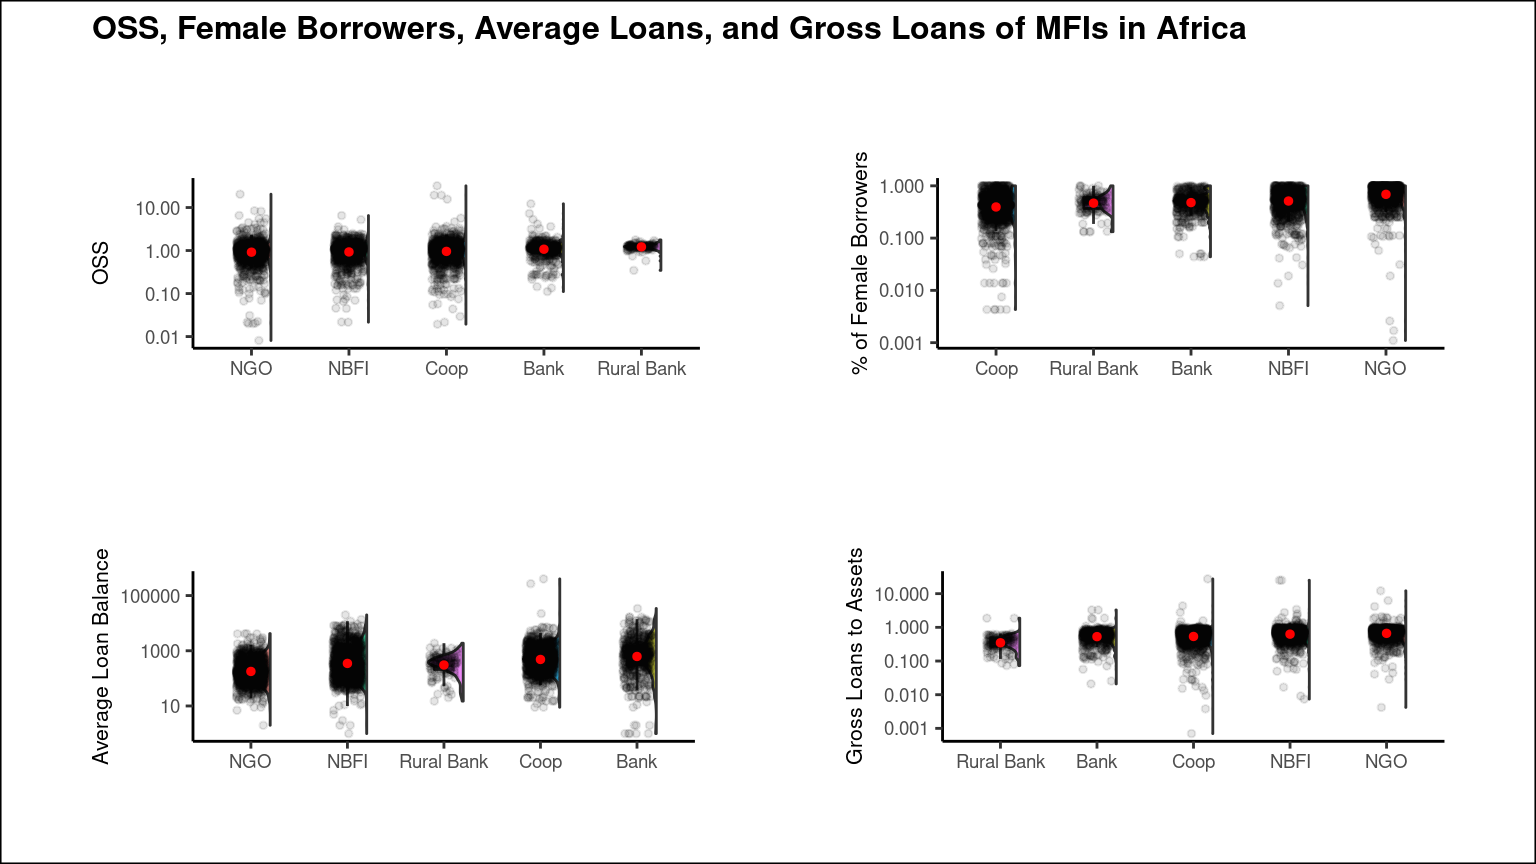
\includegraphics{_main_files/figure-latex/unnamed-chunk-129-1.pdf}
\caption{\label{fig:unnamed-chunk-129}Financial Sustainability and Social Performance Metrics for MFIs in Africa}
\end{figure}

\end{landscape}

\begin{landscape}

\begin{table}[!htbp] \centering 
  \caption{Regression Output for Efficiency for Winsorized Data (Standard Errors in Brackets)} 
  \label{} 
\tiny 
\begin{tabular}{@{\extracolsep{5pt}}lD{.}{.}{-3} D{.}{.}{-3} D{.}{.}{-3} D{.}{.}{-3} D{.}{.}{-3} D{.}{.}{-3} } 
\\[-1.8ex]\hline 
\hline \\[-1.8ex] 
 & \multicolumn{6}{c}{\textit{Dependent variable:}} \\ 
\cline{2-7} 
\\[-1.8ex] & \multicolumn{6}{c}{depvar} \\ 
\\[-1.8ex] & \multicolumn{1}{c}{(1)} & \multicolumn{1}{c}{(2)} & \multicolumn{1}{c}{(3)} & \multicolumn{1}{c}{(4)} & \multicolumn{1}{c}{(5)} & \multicolumn{1}{c}{(6)}\\ 
\hline \\[-1.8ex] 
 currentlegalstatusBank &  &  &  & 0.125^{***} & -0.108^{***} & -0.077^{***} \\ 
  &  &  &  & (0.025) & (0.015) & (0.016) \\ 
  & & & & & & \\ 
 currentlegalstatusNBFI &  &  &  & 0.003 & -0.087^{***} & -0.082^{***} \\ 
  &  &  &  & (0.018) & (0.012) & (0.012) \\ 
  & & & & & & \\ 
 currentlegalstatusCoop & -0.0001 & 0.041 & 0.041 & 0.010 & -0.137^{***} & -0.126^{***} \\ 
  & (0.015) & (0.052) & (0.052) & (0.015) & (0.011) & (0.011) \\ 
  & & & & & & \\ 
 currentlegalstatusRural Bank &  &  &  & 0.066^{**} & -0.106^{***} & -0.080^{***} \\ 
  &  &  &  & (0.028) & (0.022) & (0.023) \\ 
  & & & & & & \\ 
 ageYoung & 0.003 & 0.002 & 0.002 & 0.001 & 0.001 & -0.001 \\ 
  & (0.002) & (0.005) & (0.005) & (0.003) & (0.005) & (0.005) \\ 
  & & & & & & \\ 
 ageMature & 0.005^{*} & -0.0002 & -0.0001 & 0.002 & -0.002 & -0.006 \\ 
  & (0.003) & (0.008) & (0.008) & (0.004) & (0.007) & (0.007) \\ 
  & & & & & & \\ 
 kkm & -0.002 & 0.001 & 0.001 & -0.00001 & -0.001 & -0.0002 \\ 
  & (0.001) & (0.003) & (0.003) & (0.001) & (0.002) & (0.002) \\ 
  & & & & & & \\ 
 asset\_structure & -0.078^{***} & 0.065 & 0.069 & -0.092^{***} & 0.034 & 0.024 \\ 
  & (0.020) & (0.044) & (0.045) & (0.025) & (0.041) & (0.043) \\ 
  & & & & & & \\ 
 pcrdbgdp & -0.003 & -0.020^{*} & -0.020^{*} & 0.0004 & -0.019^{***} & -0.016^{**} \\ 
  & (0.004) & (0.010) & (0.010) & (0.005) & (0.007) & (0.008) \\ 
  & & & & & & \\ 
 stmktcap & 0.005^{**} & -0.013^{***} & -0.011^{***} & 0.006^{**} & -0.0003 & 0.002 \\ 
  & (0.002) & (0.004) & (0.004) & (0.003) & (0.003) & (0.003) \\ 
  & & & & & & \\ 
 log(assets) & -0.162^{***} & 0.014 & 0.017 & -0.178^{***} & -0.034 & -0.046^{*} \\ 
  & (0.018) & (0.037) & (0.038) & (0.019) & (0.026) & (0.027) \\ 
  & & & & & & \\ 
\hline \\[-1.8ex] 
Model & Within & Within & Within & Random & Random & Random \\ 
Depvar & FinEff & SocEff & FinSocEff & FinEff & SocEff & FinSocEff \\ 
Data & Full & 3 Years and over & 5 Years and over & Full & 3 Years and over & 5 Years and over \\ 
Observations & \multicolumn{1}{c}{4,292} & \multicolumn{1}{c}{4,292} & \multicolumn{1}{c}{4,292} & \multicolumn{1}{c}{4,292} & \multicolumn{1}{c}{4,292} & \multicolumn{1}{c}{4,292} \\ 
R$^{2}$ & \multicolumn{1}{c}{0.062} & \multicolumn{1}{c}{0.043} & \multicolumn{1}{c}{0.041} & \multicolumn{1}{c}{0.132} & \multicolumn{1}{c}{0.632} & \multicolumn{1}{c}{0.627} \\ 
Adjusted R$^{2}$ & \multicolumn{1}{c}{-0.171} & \multicolumn{1}{c}{-0.196} & \multicolumn{1}{c}{-0.198} & \multicolumn{1}{c}{0.126} & \multicolumn{1}{c}{0.629} & \multicolumn{1}{c}{0.624} \\ 
F Statistic (df = 28; 3434) & \multicolumn{1}{c}{8.170$^{***}$} & \multicolumn{1}{c}{5.500$^{***}$} & \multicolumn{1}{c}{5.300$^{***}$} & \multicolumn{1}{c}{262.000$^{***}$} & \multicolumn{1}{c}{408.000$^{***}$} & \multicolumn{1}{c}{333.000$^{***}$} \\ 
\hline 
\hline \\[-1.8ex] 
\textit{Note:}  & \multicolumn{6}{r}{$^{*}$p$<$0.1; $^{**}$p$<$0.05; $^{***}$p$<$0.01} \\ 
\end{tabular} 
\end{table}

\end{landscape}

\begin{landscape}

\newpage

\hypertarget{qq-plots-for-financial-and-social-efficiency}{%
\subsection{QQ Plots for Financial and Social Efficiency}\label{qq-plots-for-financial-and-social-efficiency}}

\begin{figure}

{\centering 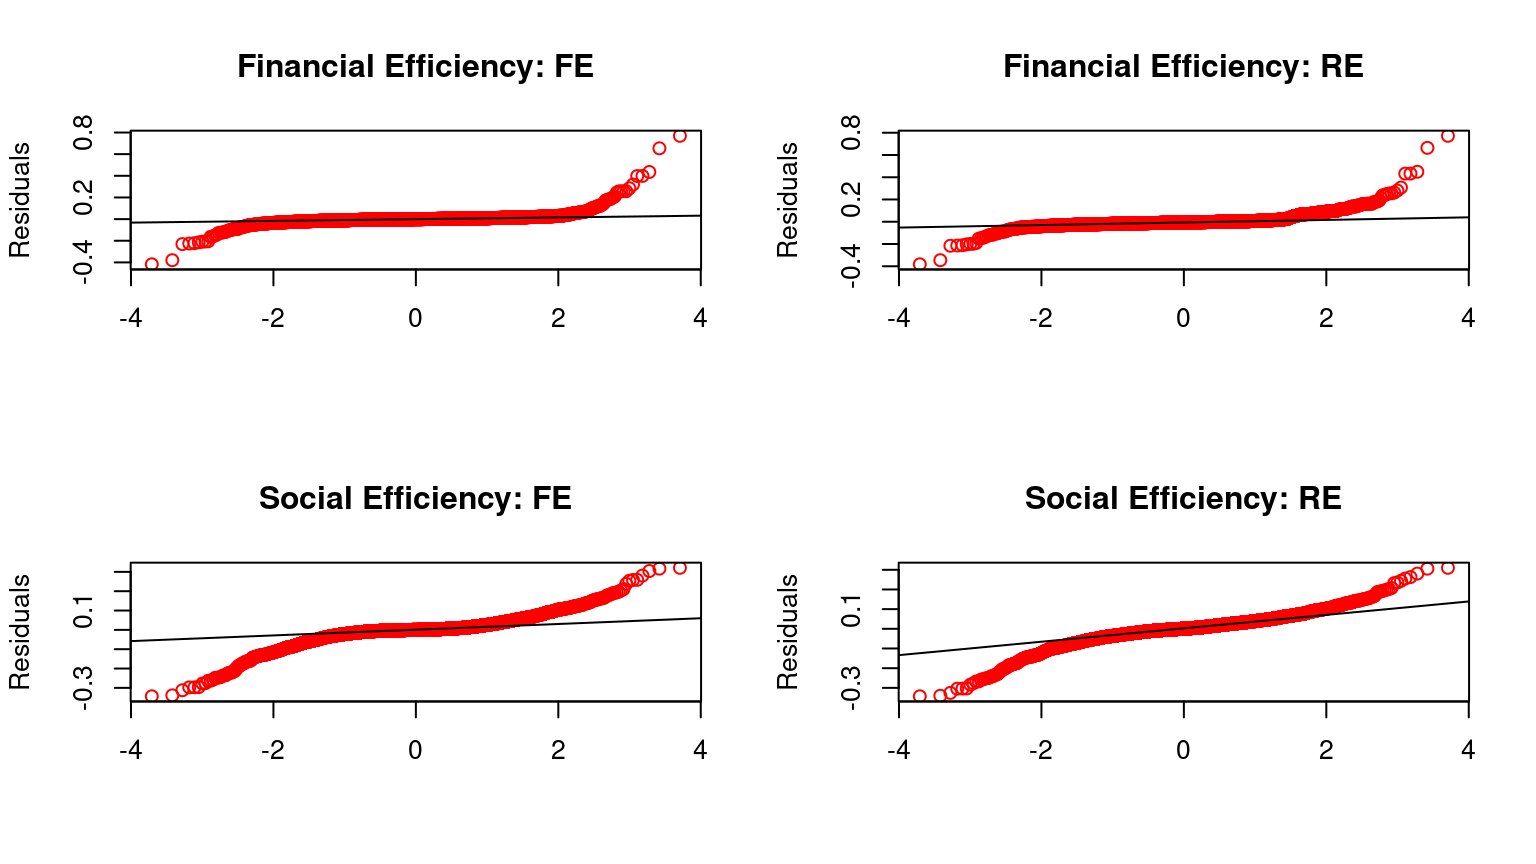
\includegraphics{_main_files/figure-latex/unnamed-chunk-133-1} 

}

\caption{residual QQ-plots for Fixed and Random Effects Regression Models}\label{fig:unnamed-chunk-133}
\end{figure}

\newpage

\hypertarget{qq-plots-financialsocial-efficiency-winsorised.}{%
\subsection{QQ-Plots, Financial/Social Efficiency (Winsorised).}\label{qq-plots-financialsocial-efficiency-winsorised.}}

\begin{figure}

{\centering 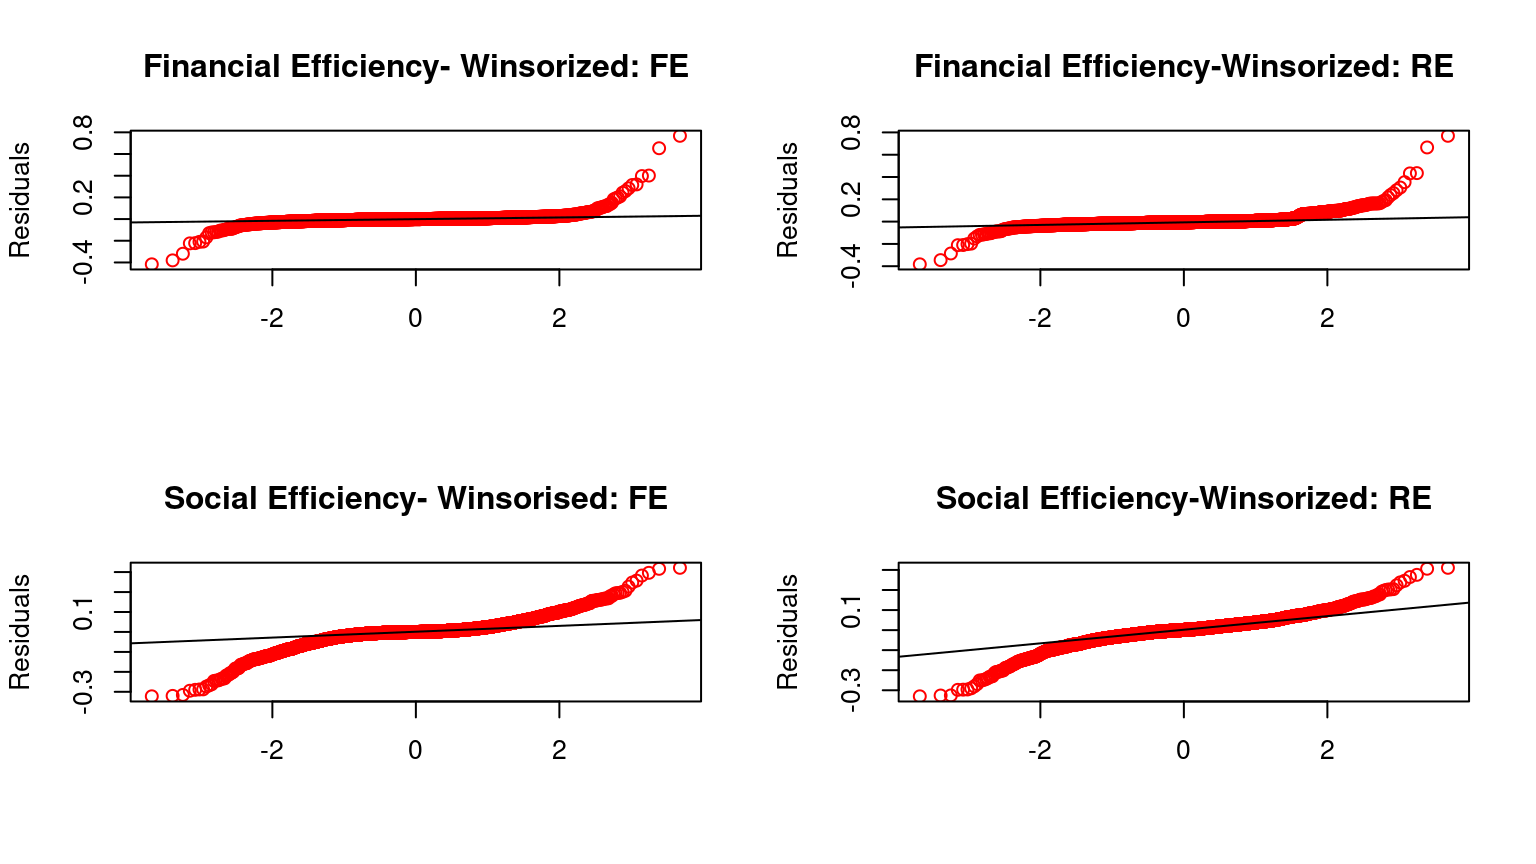
\includegraphics{_main_files/figure-latex/unnamed-chunk-134-1} 

}

\caption{residual QQ-plots for Fixed and Random Effects Regression Models}\label{fig:unnamed-chunk-134}
\end{figure}

\newpage

\hypertarget{qq-plots-for-socio-financial-efficiency}{%
\subsection{QQ-Plots for Socio-Financial Efficiency}\label{qq-plots-for-socio-financial-efficiency}}

\begin{figure}

{\centering 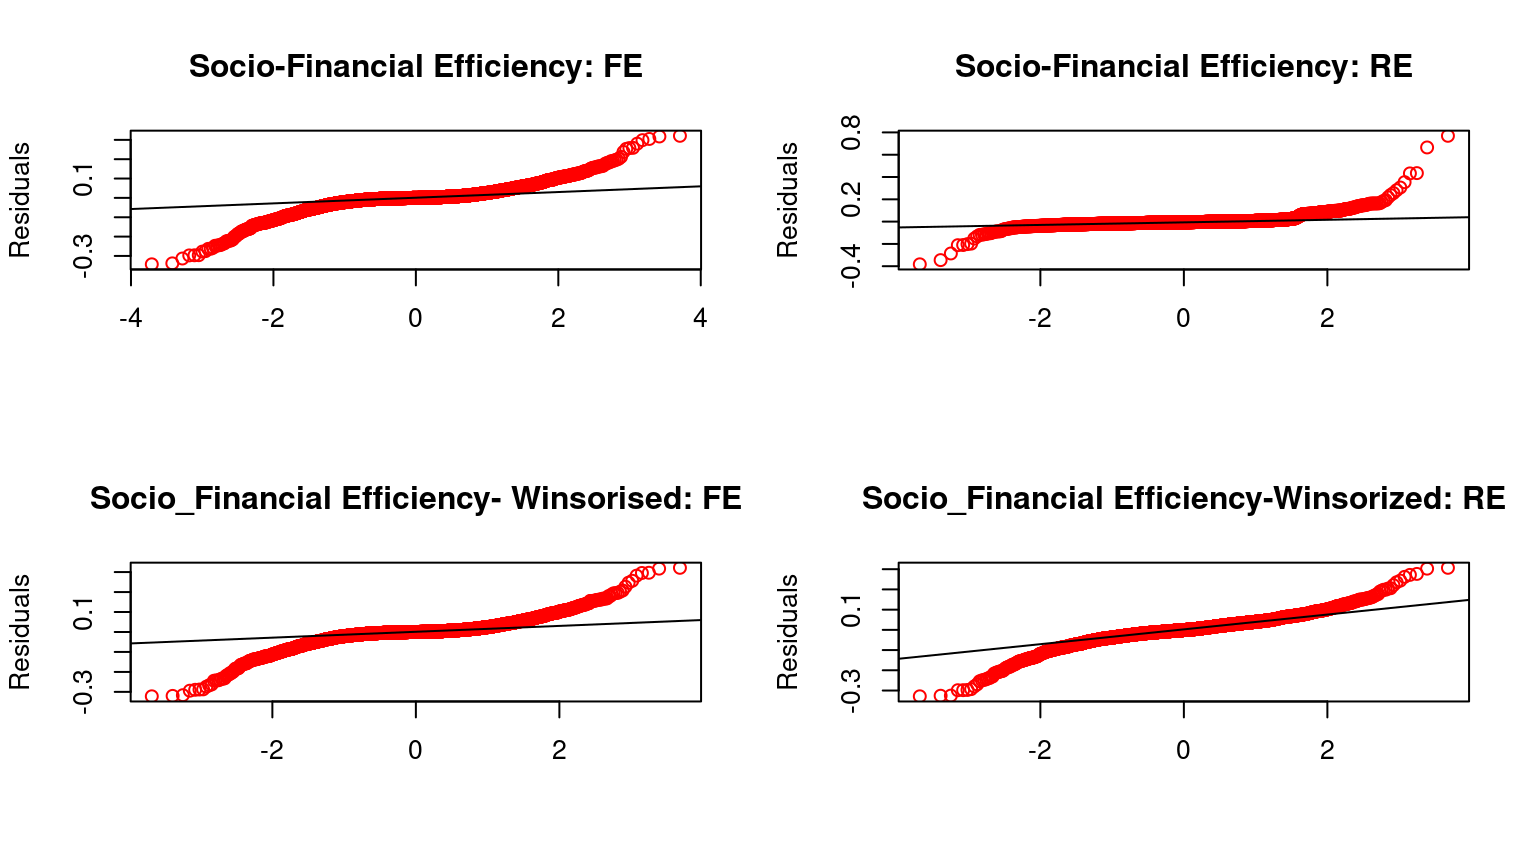
\includegraphics{_main_files/figure-latex/unnamed-chunk-135-1} 

}

\caption{residual QQ-plots for Fixed and Random Effects Regression Models}\label{fig:unnamed-chunk-135}
\end{figure}

\end{landscape}

\hypertarget{the-double-bottom-line-goal-of-microfinance-institutions-in-africa}{%
\chapter{The Double Bottom Line Goal of Microfinance Institutions in Africa}\label{the-double-bottom-line-goal-of-microfinance-institutions-in-africa}}

\minitoc 
\chaptermark{Achievement of Dual Objectives by MFIs}

\newpage

\begin{center}

\textbf{ABSTRACT}

\end{center}

\begin{quote}
This article uses data from the World Bank to examine how microfinance institutions (MFIs) in Africa fare in pursuing the double bottom line - meeting financial and social objectives. It also looks into the factors associated with the capacity of MFIs to achieve the double bottom line. We capture social performance using the per cent of female borrowers while operational self-sufficiency proxies financial performance. The results show that most MFIs in Africa attain the dual objectives, at 35.88\% compared to the 14.76\% who fail in both missions. Interestingly, rural banks and NGOs are more likely to achieve the dual goals than banks, NBFIs and credit unions. Age, size, capital markets development, institutional quality, legal tradition, and legal status are the significant determinants of how MFIs fare in the effort to attain joint financial and social objectives. The results remain robust after removing outliers.
\end{quote}

vspace\{10mm\}

\textbf{Key Words}: Microfinance, Efficiency, Social, Financial, Performance, Africa.

\vspace{5mm}

\textbf{JEL Classification}: G210, G230

\newpage

\hypertarget{background-2}{%
\section{Background}\label{background-2}}

Microfinance Institutions (MFIs) set out to reach out to the financially excluded people with little emphasis on making profits in the early stages. However, the rise of neoliberalism has seen an increasing number of MFIs also pursuing a financial returns goal. The argument is that financially sustainable MFIs could better serve the financially excluded without over-reliance on volatile donor funds and uncertain state subsidies \autocite{garmaise2013cheap,d2017aid,armendariz2013subsidy,d2013unsubsidized}. Consequently, most modern MFIs globally are hybrid firms that have a dual objective of reaching out to the financially excluded while striving for financial sustainability \autocite{d2017ngos}. Like most hybrid firms, MFIs face a challenge in striking a balance between the pursuit of profit and the outreach to the poor, their chief social mission \autocite{jia2016commercialization,d2013unsubsidized}. When the financial goals of an MFI come at the expense of social goals, the MFI is said to have experienced mission drift \autocite{mersland2010microfinance}.

While some researchers posit that it is possible to profitably offer financial services to the poor, financially excluded individuals \autocite{kodongo2013individual}, others hold the opposite view \autocite{mersland2010microfinance}. The opponents argue that offering financial services to indigent clients is a high cost, high-risk business owing to the high costs of administering small loans that affer no economies of scale \autocite{ledgerwood2006transforming}. Similarly, the poor, more so in Africa, lack collateral, are often located in remote geographic areas, lack financial literacy, and engage in informal economic activity, making it hard to track finances to assess their creditworthiness. It is against this background that most initial MFIs like the Grameen Bank in Bangladesh ran on the welfare model, emphasising outreach to the poor even at the expense of profitability. MFIs following the welfare approach had substantial backing in donor funds and state subsidies \autocite{armendariz2013subsidy}.

As noted, the rise of neo-liberalism after the cold war led to a paradigm shift towards financial sustainability \autocite{bateman2010doesn}. The transition has accompanied a reduction in the level of donations and subsidies, compelling many MFIs to also strive for financial sustainability \autocite{d2017ngos}. The shift has forced MFIs to pursue a double bottom line, that is, achieve social goals while ensuring financial viability \autocite{ramus2017}. The trend has been the conversion of NGO, welfare MFIs, to the commercial, profit-oriented microfinance model. As noted, many researchers hold differing viewpoints regarding the suitability of MFIs pursuing the dual objectives. Some researchers argue that seeking profits is detrimental to the social mandate of reaching the unbanked due to the possibility of ``mission drift'', where MFIs seek profits to the detriment of their social mandate. If MFIs drift from their mission, then they risk the legitimacy that affords them a favourable legal framework from the state and earns them goodwill from stakeholders \autocite{market2018global}. Other researchers believe that financial sustainability makes MFIs better serve the excluded. \textcite{mersland2010microfinance} conducted some empirical analysis and concluded that the pursuit of profits by MFIs leads to a lower level of outreach, referred to as ``mission drift''. On the contrary, other researchers claim that financially sustainable MFIs reach more financially excluded people, a phenomenon dubbed ``mission expansion'' \autocite{mersland2010microfinance}.

In this article, we pursue two issues. First, we explore the levels of combined financial and social performance of MFIs in Africa. Secondly, we examine the factors behind the level of joint financial and social performance of MFIs in Africa. We capture financial performance using the operational self-sufficiency, OSS \footnote{\(OSS = \frac{operating revenue}{expenses on funding, loan loss provisions, and operations}\) \autocite{market2018global}}, while the per cent of female borrowers proxies social performance. The literature shows that the majority of the financially excluded are women and rural dwellers in Africa \footnote{We did not include MIX data on lending to rural dwellers as it had a large proportion of missing values.}. Specifically, the study takes MFIs with an OSS of at least one to be financially sustainable. Likewise, MFIs that have at least 50\% of female borrowers have succeeded socially in reaching out to the financially excluded. Following \textcite{chattopadhyay2017applicability}, we develop a matrix to capture the extent to which MFIs achieve the dual objectives as shown in Table 6.1 below.

The article contributes to the existing literature in two main ways. First, the research work documents the extent of financial and social performance of MFIs in Africa, and thus contributes to the debate on mission drift versus mission expansion. Secondly and critically, while much research examines the consequences of the transformation of MFIs \autocite{fernando2004micro,hishigsuren2006transformation,d2017ngos,ramus2017}, few delve into the factors that drive the success or failure in the dual missions of MFIs as this paper does. Instead, much of the currently available research examines the effects of MFI transformation on financial sustainability and social missions with each outcome examined in isolation. The other strand examines trade-offs between the financial and social performance of MFIs without delving into the drivers of the extent of the trade-offs. Hence, this research contributes to the existing literature by examining the determinants of the achievement of twin objectives.

While much of the research has dwelt on the trade-offs or synergies between the two schools, little of it investigates why some MFIs would differ in achieving the dual objectives. \textcite{quayes2019probability} is the closest research to our contribution. In their study, they examine the probability of an MFI achieving financial sustainability. The presumption is that financial sustainability is a proxy for social outreach, meaning that the researchers lean towards microfinance's financial systems approach. The researchers conclude that the probability of financial sustainability positively affects depth of outreach, breadth of outreach, and outreach to women. The researchers do not examine the financial and social objectives together as we do in this study.

The classification in Table 6.1 shows four categories of MFIs based on achieving both financial and social goals. In class 1, the MFIs have failed both socially and financially. These are MFIs with a share of women borrowers lower than 50\% of the total borrowers and a operational self-sufficiency (OSS) less than unity. MFIs in this class risk losing legitimacy, fail to attract donations, subsidies, and being loss-making ultimately collapse. There is little literature that examines situations where MFIs fail in the twin objectives reflecting the expectations that an MFI should at least exhibit positive social influence even if it does not fare well financially.

In class 2, the MFIs succeed socially in reaching the unbanked but fail in financial sustainability. The welfare approach (NGO-Model) subscribes to this approach \autocite{kodongo2013individual}. Although some NGOs do turn profits, this class of MFIs is a prime candidate for donations and subsidies and illustrates, as welfarists do, that financial sustainability of MFIs is not compatible with social goals. However, better financial management could allow this class of MFIs to improve their financial sustainability without trading off social goals. The financial sustainability school argues that it is possible to push these MFIs to financial sustainability without losing sight of their social mandate.

In category three, the MFIs succeed financially but fail in the social mission. This category contains MFIs that are subject to mission drift, confirming the welfare school's view on the incompatibility between profitability and social outreach \autocite{mersland2010microfinance,mia2017mission}. The MFIs in this category risk their legitimacy but could survive as they operate a commercial model like mainstream commercial banks. Most cooperatives, NBFIs, and commercial banks in our dataset fall into this category, calling into question the viability of the coexistence of the profit-oriented approach to microfinance and the need to reach out to the financially excluded. NGOs form a small proportion of this group showing their relevance in microfinance. Finally, some MFIs succeed both financially and socially, which is desirable. This category points to MFIs from which mission expansion could arise. This class presents an ideal scenario for the win-win approach to microfinance that argues for the possibility of pursuing both objectives. This class also serves the financial sustainability school well, although its viability is controversial.

This current study fits within the agency theory. The entry of private capital into microfinance is bound to raise a conflict between providing appropriate and affordable financial services to the financially excluded and pursuing profits \autocite{miller2011angel}.While equity and debt-holders may favour financial inclusion, maximising returns on their investments comes first, unless blended finance is the financing model in use. Blended finance allows MFIs to use private capital to do social good without an overemphasis on profitability. Even where agency conflicts adversely affect the provision of financial services to the poor, it is hard for MFIs to keep off the financial sustainability push. The institutional theory sheds light here, where the institutional environment has a greater influence on the adoption of institutional structures than market pressures. In this respect, pressures from donor agencies may still cause more MFIs to convert to the commercial model even where evidence shows that the conversion may be detrimental to the social goal of availing financial services to the financially excluded.

There exist MFIs that serve different segments of society. For instance, cooperatives serve a limited geographic range, targeting people with a common bond like employment. Rural banks also serve limited geographic areas in remote rural locations. MFIs registered as commercial banks and NBFIs serve relatively better off, but still poor people not served by mainstream financial intermediaries. Consequently, some researchers argument that we should allow a broad range of MFIs to exist to serve different market segments appears valid \autocites[by][]{morduch1999microfinance,morduch2000microfinance}. Supporting this point, \textcite{morduch2019challenges} argue that if there were no market failures in the credit market that leaves out a segment of the population unbanked, NGOs would not exist as commercial banks because other MFIs would already have filled the gap. It follows, therefore, that the call to do away with NGOs does not augur well for the financially excluded. These viewpoints call to question the validity and relevance of the debate on the pros and cons of microfinance institutions' transformation across the globe. What is critical, it seems to us, is to evaluate factors relevant for MFIs to achieve their financial and social goals as a basis for crafting policy support. Moreover, the management of MFIs would better adjust their strategies when aware of the issues that hinder or facilitate the achievement of the twin objectives.

The rest of the research proceeds as follows. In the next section, we summarise the study results followed by a description of the econometric model. We then discuss the results of the regression in detail and then conclude the report.

\begin{table}

\caption{\label{tab:unnamed-chunk-136}Classification Matrix: Joint Financial and Social Performance of MFIs}
\centering
\begin{tabular}[t]{llll}
\toprule
  &   & Achieves\_Financial\_Goals? & Achieves\_Financial\_Goals?\\
\midrule
 &  & YES & NO\\
Achieves\_Social\_Goals? & YES & Class 4 (SS) & Class 2 (FS)\\
Achieves\_Social\_Goals? & NO & Class 3 (SF) & Class 1 (FF)\\
\bottomrule
\multicolumn{4}{l}{\rule{0pt}{1em}\textit{Source: }}\\
\multicolumn{4}{l}{\rule{0pt}{1em}Adapted from Chattopadhyay, Manojit, and Subrata Kumar Mitra (2017)}\\
\multicolumn{4}{l}{\rule{0pt}{1em}\textit{Note}}\\
\multicolumn{4}{l}{\rule{0pt}{1em}\textsuperscript{1} In labelling the classes, we start with financial sustainability followed by social performance.}\\
\multicolumn{4}{l}{\rule{0pt}{1em}\textsuperscript{2} The letters F and S stand for Fails (F) and Succeeds (S), respectively.}\\
\multicolumn{4}{l}{\rule{0pt}{1em}\textsuperscript{3} For instance, FS means the MFI fails (F) financially but succeeds (S) socially.}\\
\end{tabular}
\end{table}

\hypertarget{summary-of-results-3}{%
\section{Summary of Results}\label{summary-of-results-3}}

Overall, MFIs in Africa achieve both outreach (social goals) and financial goals more than they fail in both objectives at 35.88\% and 14.76\%, respectively. 25.55\% of MFIs succeed financially but fail socially by not reaching out adequately to the financially excluded. This result is indicative of mission drift. Another 23.80\% fail financially but fare well in their social mandate of reaching the financially excluded. Broken down further, 48.59\% of NGOs and 52.17\% of rural banks attain both financial and social goals, as against 7.34\% and 0.72\%, respectively, that fail in both. The proportions of banks, NBFIs, and credit unions that succeed financially and socially are 45.72\%, 36.87\%, and 17.73\%. Those that fail in both objectives are 6.3\%, 13.51\%, and 27.61\%, respectively. NGOs have the lowest proportion of MFIs that experience mission drift by meeting financial goals while failing socially at 7.66\%. On the other hand, credit unions have the second-highest mission drift at 40.43\%, after rural banks at 43.48\%.

The regression results show that the significant factors in determining the extent of achieving both objectives are age, size, capital markets development, institutional quality, legal tradition, and legal status. Specifically, mature MFIs are less prone to mission drift given they are more likely to fail both financially and socially than succeed in one objective while failing in the other. Larger MFIs, on the other hand, are more likely to succeed financially and fail socially than they are to fail in both objectives. Similarly, large MFIs are more likely to succeed in both goals than to fail. The results are indicative of larger MFIs being more prone to mission drift. A higher level of capital markets development and governance corresponds to a higher chance of failing in both objectives, probably due to low demand for microfinance in countries with well developed mainstream financial systems.

Similarly, MFIs in legal traditions other than common law are more likely to fail in both objectives. The result probably connotes weak legal and infrastructural support that suppresses the development of mainstream and alternative financial systems like microfinance. Finally, the legal status outcome shows that NGOs are less likely to succeed financially while failing socially. However, NGOs are more likely than other legal forms to fail socially while succeeding financially and succeeding in both objectives. The results show that commercial forms of MFIs are more prone to mission drift.

\hypertarget{the-model}{%
\section{The Model}\label{the-model}}

The article uses the multinomial logit model, given that our dependent variable is discrete and error terms may not be normally distributed \autocite{cramer2002origins}. In the model, NGOs take a zero code, with commercial banks, NBFIs, credit unions, and Rural Banks coded one, two, three, and four, respectively. The following section lays out and describes the models, variables, and data sources.

\hypertarget{the-model-variables-description-and-data-sources-1}{%
\subsection{The Model, Variables Description and Data Sources}\label{the-model-variables-description-and-data-sources-1}}

We run a multinomial logit model on a panel dataset of 705 MFIs in Africa. The multinomial logit model is an extension of the logit model, and hence we start by describing the logit model. Assuming the error term \(\epsilon\) follows a logistic distribution \autocite{czepiel2002maximum}, we have:

\begin{equation}
y_{it} = log(\frac{p_{it}}{(1-p_{it})} ) = \alpha + x_{it} + \varepsilon_{it}
\end{equation}

where,

\begin{equation}
p_{it}  =  \frac{1}{1 +  e^{- z_{it} } } 
\end{equation}

and

\begin{equation}
1 + p_{it}  =  \frac{1}{1 +  e^{z_{it} } }
\end{equation}

for \(z_{it} = f(x_{it})\)

In the model, \(y_{it}\) is the current legal status of the MFI, the dependent variable, that is, the dependent variable is a dummy with NGOs, the base outcome (coded zero), and other legal traditions take a code of one. The symbol \(x_{it}\) represents a vector of independent variables: age, size, capital market development, legal tradition, GDP growth rate, and institutional quality. Additionally, we include year dummies to cater for the trends towards commercialisation.

The multinomial logit model extends the binary logit model to more than two unordered levels (discrete choices). The data at hand meets the requirements for running a multinomial logit model as the dependent variable (the legal status of each MFI) has one outcome for each case. Also, the independent variables do not predict the dependent variable perfectly \autocite{petrucci2009primer}. Suppose we have a dependent variable \(y\) consisting of \(K\) choices for \(K \geqslant 2\). Further, let the independent variables be \(x_1, x_2,………. x_n\), then we can specify the multinomial logit model as follows.

\begin{equation}
log(\frac{prob(k/X)}{prob(K/X)}) =   \beta_{0}^{k}  x_{0}  + \beta_{1}^{k}  x_{1} +  \cdots + \beta_{p}^{k}  x_{p}
\end{equation}

for \(k = 1 \cdots K-1\)

\(y\) is the dependent variable, in this case, one of NGO, commercial bank, NBFI, credit union or rural bank.

\(x\) is a vector of independent variables.

If \(K>2\), then we have a multinomial logit with \(K-1\) set of equations. Where \(K=2\), the model is the binary logit model denoted in equation one (1) where we have one equation. Note that in this case, we have arbitrarily assigned the last category (K) as the reference. Any other group can serve as a reference and hence not be part of the equations set.

One of the significant drawbacks of the multinomial logit is the violation of the assumption of the independence of irrelevant alternatives (IIA). \textcite{cheng2007testing} ) illustrate this assumption using the blue bus-red bus example. If the choice between car transport and a red bus, and given that the probability of choosing a bus is \(0.8\), and \(0.2\) for a car, then the bus's odds over car transport is 4. Suppose we introduce a third alternative, the blue bus. If the probabilities of choosing a red bus, blue bus, and car transport are \(0.6\), \(0.25\), \(0.15\), respectively, the assumption holds since the odds of selecting a red bus over a car are still \(4\). If the odds are different from \(4\), then the model violates the IIA, and the multinomial model is not fit for the data. In our case, we plausibly see the assumption holding because the legal status of an individual MFI is independent of the legal status of other MFIs. Table 6.2 (next page) describes the variables in detail.

\hypertarget{variables-description-and-data-sources}{%
\subsection{Variables Description and Data Sources}\label{variables-description-and-data-sources}}

The dependent variable is a dummy with four levels that capture how well MFIs achieve financial and social objectives. The firm-level independent variables are the legal status, age and size of the MFIs. The legal tradition, institutional quality, private credit to GDP, stock market to GDP, and GDP growth rates capture country-level macro-factors.

As illustrated in Table 6.1, we construct the dependent variable using the combination of the percentage of women borrowers and operational self-sufficiency (OSS). Lending to women proxies the social performance of MFIs, with success being where an MFI has women clients comprising 50\% or more of the total borrowers. An OSS of at least one indicates a financially sustainable MFI. We then generate four categories starting from MFIs that succeed in both financial and social metrics on one extreme and those that fail in both on the other. In between are MFIs that succeed in one of the metrics but fail in the other. Apart from the proposition by \textcite{chattopadhyay2017applicability}, little research has applied this approach to examine the joint financial and social efficiency of MFIs.

As noted, some legal forms of MFIs restrict the capacity of MFIs to emphasise financial or social goals. NGOs are an extreme case where donors and stakeholders expect that they are more socially oriented. Their degree of social orientation is the source of legitimacy and justifies continued donor and state support. In Africa, rural banks serve a niche market that is most prone to financial exclusion and hence are expected to focus on social performance over and above financial performance. On the other hand, cooperatives are member-oriented and may not have room to improve their social outlook unless by recruiting more diverse group members. In countries and areas where people suffer financial exclusion, joining a cooperative is out of the question given their low-income status, which leads to their financial exclusion in the first place \autocite{demirguc2018global}. The exception is farmers cooperatives that pool together smallholder farmers to gain scale economies in the procurement of inputs and sale of produce \autocite{porter1987economic}. Commercial banks and NBFIs tend to have more external capital, and agency conflicts may arise between managers who want to optimise financial and social objectives and providers of funds who may chiefly focus on financial returns. An exceptional case is that of blended finance, where providers of funds do so knowing that achieving social goals is equally critical.

The age and size of an MFI go together in explaining the firm-level factors that drive the achievement of the twin objectives. Mature MFIs tend to be larger (see Figure 6.1). Following the institutional theory, large, mature MFIs are less likely to succumb to donors and other stakeholders' pressures to attain financial sustainability \autocite{d2017aid}. Alternatively, larger and more sTable 6.MFIs have more resources to afford to offer the poor financial services even as donations subside \autocite{d2013unsubsidized}. As \textcite{mersland2010microfinance} argue, such MFIs could offer financial services to the relatively well-off at market rates, allowing them to cross-subsidize services to the financially excluded. In such a scenario, \textcite{mersland2010microfinance} argue that the conversion of MFIs to the commercial model is likely to lead to ``mission expansion'' as opposed to ``mission drift''.

The country-level factors address the macro-environment. For example, researchers associate the legal tradition with the financial system's development \autocite{schnyder2018twenty}. Common law and civil law traditions dominate in Africa, with the former exhibiting a higher financial development levels \autocite{la2013law}. People in countries with higher quality of institutional development are more likely to access the mainstream financial system \autocite{allen2013resolving,allen2014african} and demand fewer microfinance services. Likewise, countries with better institutional quality have better developed financial system, which lowers the demand for microfinance. The country's level of financial development reflects in the private credit to GDP and stock markets capitalization to GDP. Better developed financial markets imply higher access and use of financial services and lower financial exclusion chances. The result is a lower demand for microfinance resulting in poor financial and social performance by MFIs \autocite{allen2013resolving,allen2014african}.

Finally, the GDP growth rate reflects the health of the economy. With more output, people are likely to have higher incomes over time, making them demand financial services like savings and credit to smooth consumption, for example \autocite{ahlin2011does,buera2021macroeconomics}. As described in Table 6.2, the data comes from the World Bank. The firms level data is from the MIX market. The country-level data is from three chief sources: the World Development Indicators (WDI), the Worldwide Governance Indicators (WGI), and the Global Financial Development Database (GFDD). Table 6.2 shows a description of the variables employed in the study.

\begin{table}

\caption{\label{tab:unnamed-chunk-141}Description of Variables}
\centering
\fontsize{9}{11}\selectfont
\begin{tabu} to \linewidth {>{\raggedright}X}
\toprule
Variable\_Description\\
\midrule
1. Current Legal Status: This is the dependent variable. For logit and probit models, we create a dummy with the MFIs following the NGO Model getting a code of zero, and one in the case of non-bank financial institutions (NBFIs), rural banks, and credit unions/ cooperatives. We assign codes of zero to four for the multinomial logit model for NGOs, Banks, NBFIs, Cooperatives and Rural Banks, respectively. The data are available from the Microfinance Information Exchange, MIX (See source on note 1).\\
\\
2.  Age: The period in which the MFI has been in operation. MFIs fall into one of three groups: new (1-4 years), young (4-8 years), and mature (over 8 years). The data are available from MIX.\\
\\
3. Legal Tradition (Legal): The indicator is a dummy variable with common law countries coded 0, civil law countries 1, and 2 otherwise as per the classification by Oto-Peralías and Romero-Ávila (2014).\\
\addlinespace
\\
4. Size (Log of Total Assets): We proxy the size of MFI with the natural logarithm of total assets, again using MIX data.\\
\\
5. Governance/ Institutional Quality (KKM): We take the first principal component of the WGI developed by Daniel Kaufmann, Aart Kraay and Massimo Mastruzzi (KKM) available on the World Bank's Worldwide Governance Indicators, WGI (See source on note 3).\\
\\
\addlinespace
6. Private Credit to GDP: We capture the total amount of credit advanced to the private sector by financial intermediaries as a proxy for capital markets development concerning the banking sector following Ito and Kawai (2018). The data source is the Global Financial Development Database (GFDD) of the World Bank (See note 4).\\
\\
7. Stock market capitalisation to GDP: We capture the  extent of stock market development using the ratio of stock market capitalisation to GDP to proxy how firms can raise equity capital. Although Africa's equity markets are thin, some relatively large stock markets like South Africa, Kenya, and Ghana exist. The data are from the GFDD.\\
\\
8. GDP annual growth rate (GDP): This is the year on year growth in output adjusted for inflation and sourced from the World Development Indicators (WDI) (See note 2).\\
\addlinespace
\\
\bottomrule
\multicolumn{1}{l}{\rule{0pt}{1em}\textit{Source: }}\\
\multicolumn{1}{l}{\rule{0pt}{1em}Authors' construction from the literature}\\
\multicolumn{1}{l}{\rule{0pt}{1em}\textit{Notes}}\\
\multicolumn{1}{l}{\rule{0pt}{1em}\textsuperscript{1} MIX Database on www.themix.org and https://datacatalog.worldbank.org/dataset/mix-market}\\
\multicolumn{1}{l}{\rule{0pt}{1em}\textsuperscript{2} WDI on https://databank.worldbank.org/source/world-development-indicators.}\\
\multicolumn{1}{l}{\rule{0pt}{1em}\textsuperscript{3} WGI/ KKM on https://databank.worldbank.org/source/worldwide-governance-indicators.}\\
\multicolumn{1}{l}{\rule{0pt}{1em}\textsuperscript{4} GFDD on https://www.worldbank.org/en/publication/gfdr/data/global-financial-development-database}\\
\end{tabu}
\end{table}

\hypertarget{results-2}{%
\section{Results}\label{results-2}}

In this section, we explore and describe the data, followed by a discussion of the output from the regression analysis.

\hypertarget{exploratory-data-analysis-and-data-visualization}{%
\subsection{Exploratory Data Analysis and Data Visualization}\label{exploratory-data-analysis-and-data-visualization}}

\hypertarget{summary-statistics-2}{%
\subsubsection{Summary Statistics}\label{summary-statistics-2}}

Figure 6.1, Figure 6.2, and Tables 3 and 4 show a breakdown of the extent to which MFIs in Africa meet the dual financial and social objectives. Figure 6.1 shows that most MFIs in the sample achieve both financial goals with only a small proportion failing in both mandates. A marginally higher proportion of MFIs succeed financially while failing socially than those that fail financially while succeeding socially. The result could indicate that mission drift is not as widespread and that there is an even chance that an MFI will experience mission drift or not. The result goes against the welfare model of microfinance \autocite{d2017ngos}. However, a clearer picture emerges when we break down the outcome by the legal status of MFIs in Figure 6.2.

Panel A and B of Figure 6.2 show the counts, while panel C and D show the proportions of MFIs and the extent they meet the twin objectives. Tables 3 and 4 show the respective proportions. We base the discussion on Figure 6.1 panel C and Table 6.4. The results in Panel C show that cooperatives with the lowest proportion of MFIs succeeding financially and socially at 17.7\%. Besides, they have the second lowest proportion (after rural banks with 43.5\%) of failing socially and succeeding financially at 40.4\%. By contrast, they have the lowest highest chance (after rural banks with 3.6\%) of failing financially and succeeding socially at 14.2\%. Notably, cooperatives have the highest chance of failing to meet both objectives at 27.6\%. The results illustrate the nature of cooperatives as geographically limited entities whose sole focus is on members who can make savings to qualify for loans \autocite{porter1987economic}. Not many financially excluded individuals may join cooperatives due to limited incomes and information and their situation in remote geographical locations.

\newpage

\begin{landscape}

\begin{figure}

{\centering 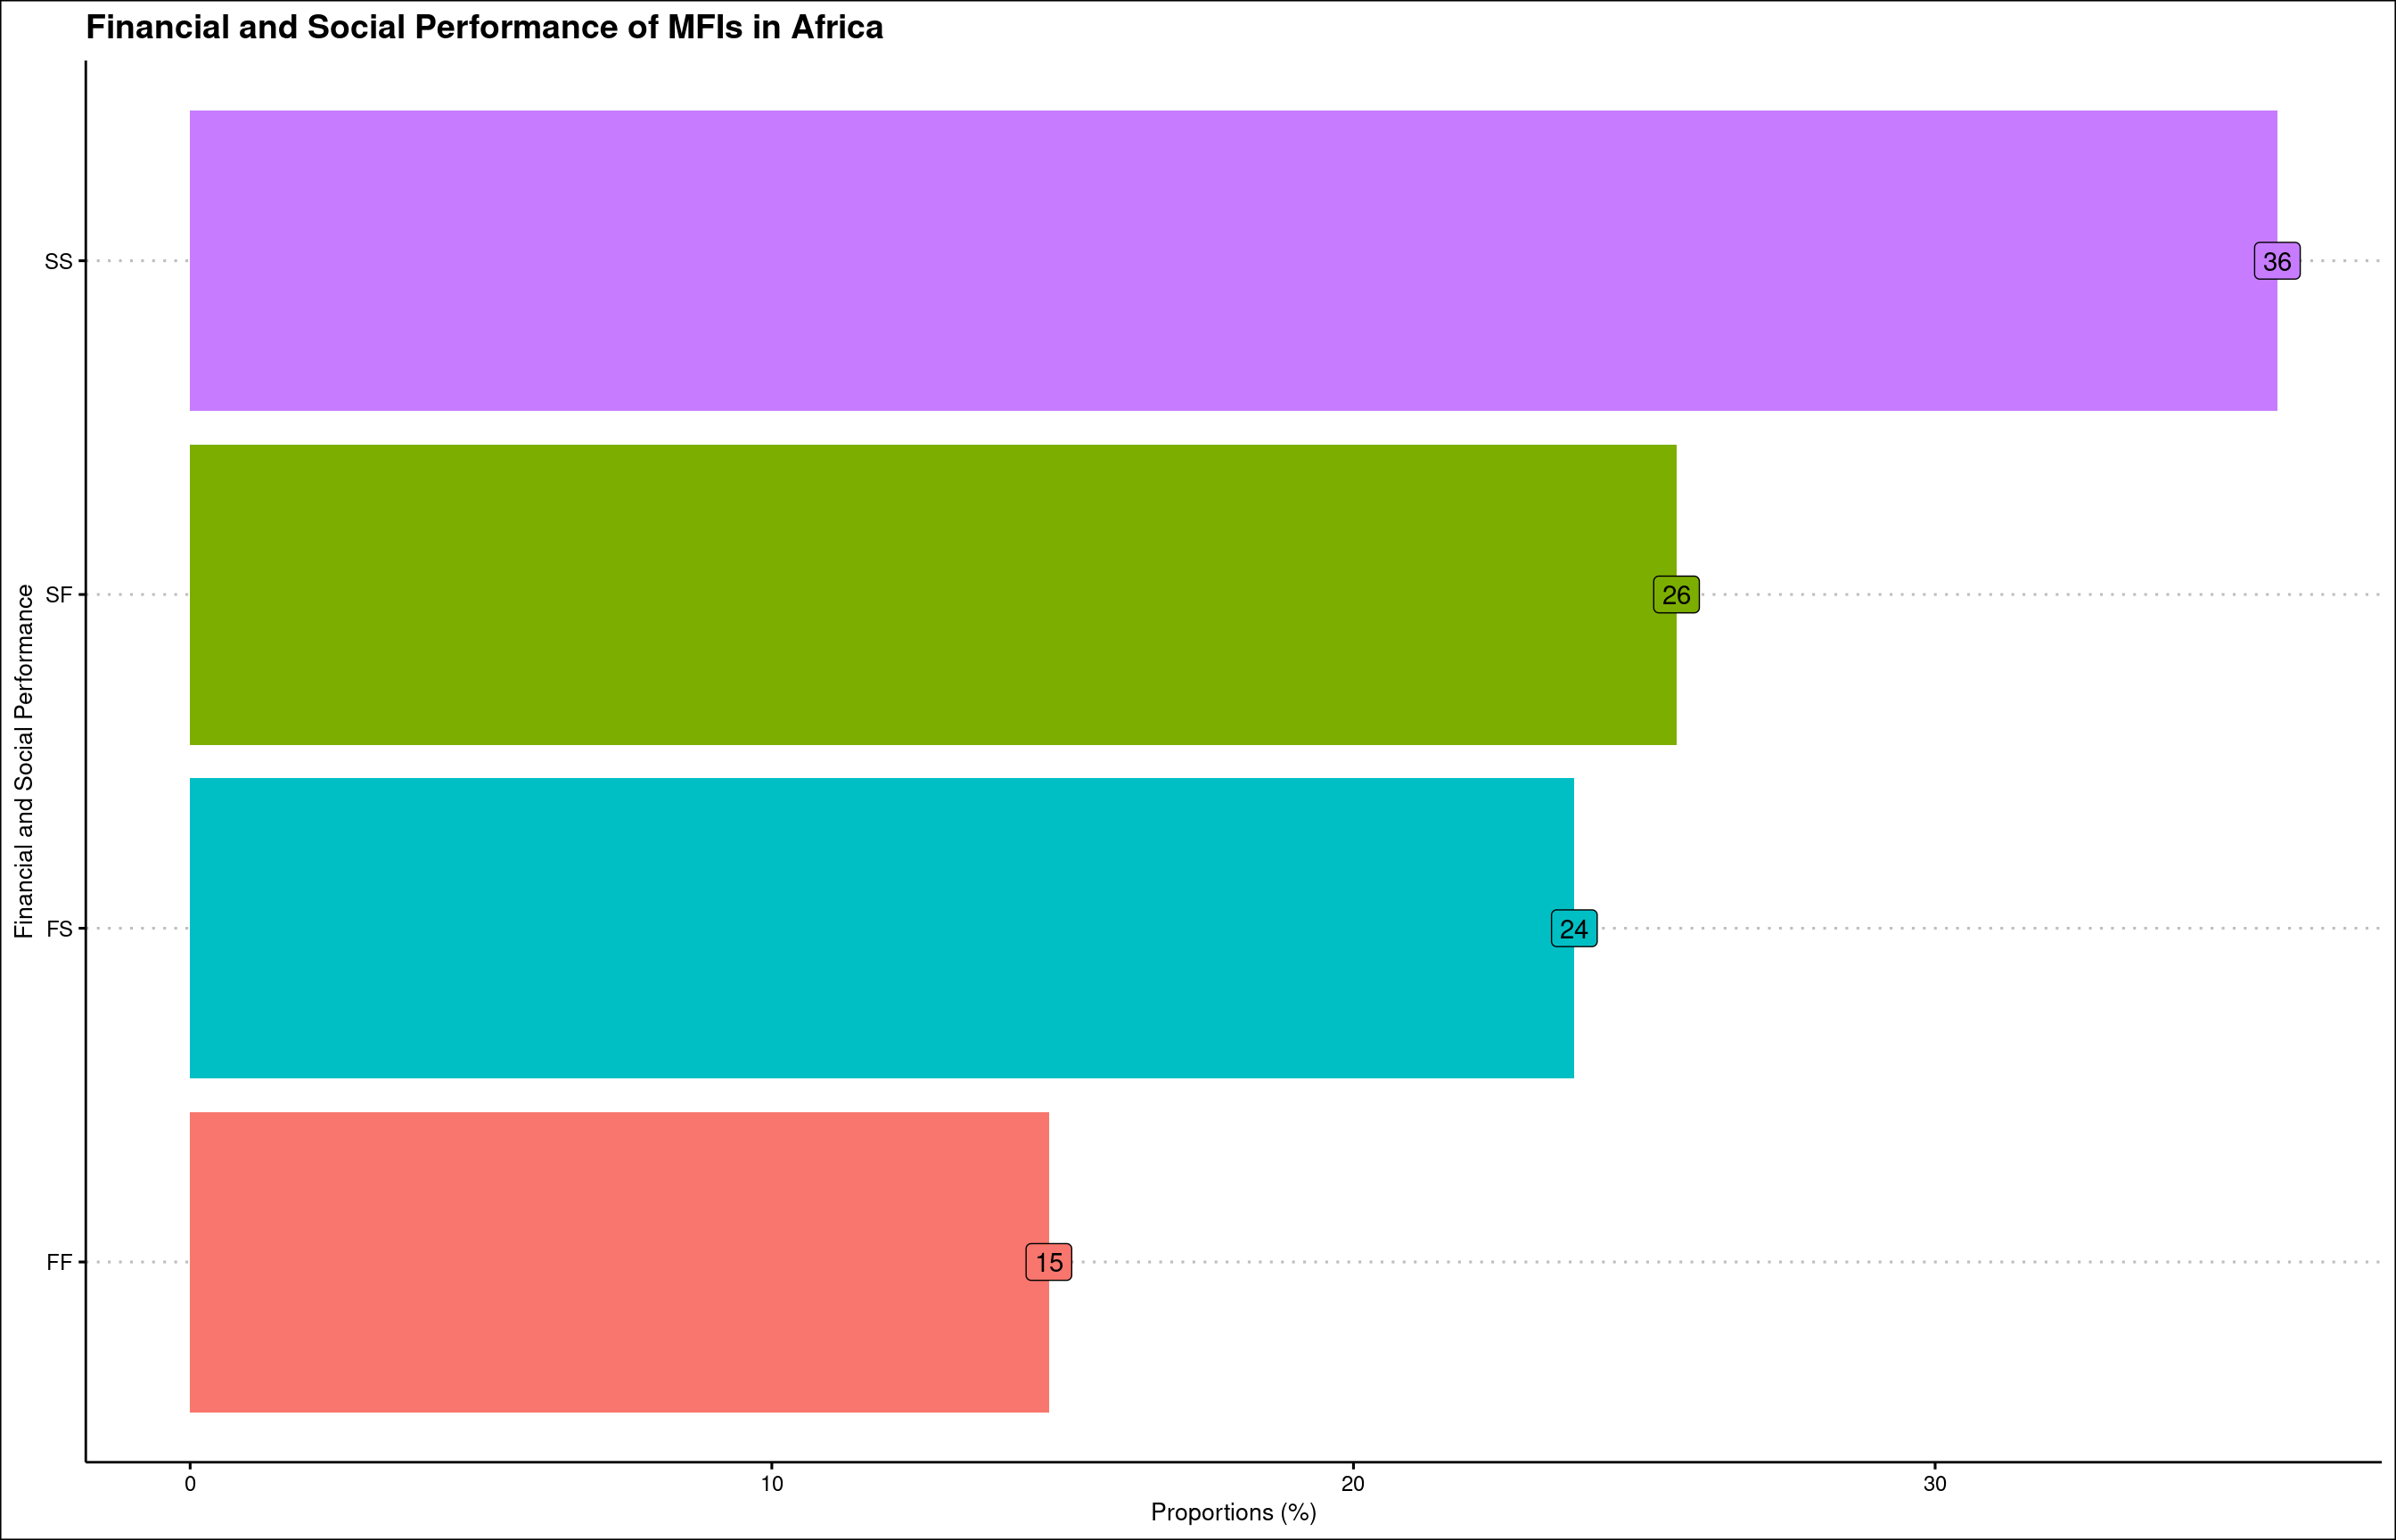
\includegraphics[width=8.8in]{_main_files/figure-latex/unnamed-chunk-142-1} 

}

\caption{Financial and Social Performance of MFIs in Africa}\label{fig:unnamed-chunk-142}
\end{figure}

\end{landscape}

\newpage

\begin{table}

\caption{\label{tab:unnamed-chunk-143}Joint Financial and Social Performance by Legal Status of MFIs in       
               Africa (row-wise)}
\centering
\fontsize{8}{10}\selectfont
\begin{tabu} to \linewidth {>{\raggedright}X>{\raggedleft}X>{\raggedleft}X>{\raggedleft}X>{\raggedleft}X>{\raggedleft}X}
\toprule
  & NGO & Bank & NBFI & Coop & Rural Bank\\
\midrule
FF & 0.1331 & 0.0552 & 0.2521 & 0.5581 & 0.0014\\
SF & 0.0802 & 0.1571 & 0.2414 & 0.4722 & 0.0491\\
FS & 0.4095 & 0.0923 & 0.3155 & 0.1784 & 0.0044\\
SS & 0.3625 & 0.1649 & 0.2832 & 0.1474 & 0.0420\\
\bottomrule
\multicolumn{6}{l}{\rule{0pt}{1em}\textit{Source: }}\\
\multicolumn{6}{l}{\rule{0pt}{1em}Authors' construction from MIX data}\\
\multicolumn{6}{l}{\rule{0pt}{1em}\textit{Note}}\\
\multicolumn{6}{l}{\rule{0pt}{1em}\textsuperscript{1} The horizontal (row) values add up to 100\%}\\
\multicolumn{6}{l}{\rule{0pt}{1em}\textsuperscript{2} We start with financial sustainability followed by social performance}\\
\multicolumn{6}{l}{\rule{0pt}{1em}\textsuperscript{3} For instance, FS means the MFI fails (F) financially but succeeds (S) socially.}\\
\multicolumn{6}{l}{\rule{0pt}{1em}\textsuperscript{4} The letters F and S stand for Fail and Succeeds, respectively}\\
\end{tabu}
\end{table}

We turn to NBFIs. NBFIs have the third-highest proportion, after NGOs and commercial banks, of MFIs that meet the twin objectives at 36.9\%. However, they have the second-highest chance, after NGOs of failing financially while succeeding socially. Similarly, after NGOs, NBFIs have the second-lowest chance of succeeding financially while failing socially at 27.2\%. NBFIs also have the second highest chance after cooperatives of failing to meet the twin objectives at 13.5\%. Also, NBFIs have the second-lowest proportion of MFIs that succeed financially while failing socially at 22.4\%. In this respect, NBFIs show some degree of social orientation. NBFIs appear to strike a balance between the extremes of failing in both objectives versus succeeding in both objectives.

NGOs have the second-highest instance of succeeding financially and socially at 48.6\% in the sample data, after rural banks. NGOs also have the highest proportion of MFIs that fail financially while succeeding socially (36.41\%). Again, NGOs have the lowest chance of succeeding financially while failing socially at 36.4\%. NGOs have the third-lowest instance (7.3\%) of failing both financially and socially after commercial banks (6.3\%) and rural banks (0.7\%). The results for NGOs illustrate their leaning towards the welfare school of prioritizing outreach over profitability. These results appear to confirm the welfare school's concerns that the explicit pursuit of profits is incompatible with the extension of financial services to the financially excluded \autocite{d2017ngos}.

Commercial banks come second after NGOs in the proportion of MFIs that succeed financially and socially at 45.7\%. However, commercial banks have the lowest chance of failing financially while succeeding socially after rural banks and cooperatives. After rural banks and cooperatives, banks are the third least likely to succeed financially while failing to meet their social objectives. Besides, commercial banks have the second-lowest instance of failing to meet both goals. Lastly, though the sample of rural banks is small, they show the highest likelihood of succeeding financially and socially and failing to achieve the twin objectives. Rural banks have the least instance of succeeding financially while failing socially, and have no instance of failing to meet both objectives. Given that rural banks specifically target the financially excluded in rural areas, it is rare that they would fail in their social mandate. However, the number of rural banks in the sample data was small and hence the results in Table 6.3.

The observations in the visualisation appear to validate the concerns by the welfare school of microfinance that, indeed, pursuing a financial return is incompatible with outreach to the financially excluded. Except for NBFIs that seem evenly spread between the different classes, the other commercial MFIs, that is, banks, cooperatives, and rural banks, are biased against social outreach. NGOs show a high degree of social orientation, are at the top when it comes to achieving the twin objectives, and come last in the class of MFIs that succeed financially and fail socially. We shall revisit this issue in the regression analysis. Finally, for profit-oriented MFIs like commercial banks, financial performance is a prerequisite for achieving social objectives. The result could be due to the lower proportion of donations and subsidies that for-profit MFIs receive \autocite{d2013unsubsidized}, which forces them to focus on financial sustainability. Only after they achieve some degree of financial sustainability do they turn their attention to achieving social goals. We visualise the data in the next section.

\hypertarget{data-visualization-1}{%
\subsubsection{Data visualization}\label{data-visualization-1}}

Figure 6.3 shows the correlation between the independent numeric variables. The highest correlation is between private credit to GDP and stock market capitalisation to GDP at 0.321. Institutional quality and private credit to GDP follow at -0.265. Overall the correlation between independent variables is not high to raise multicollinearity concerns (See Table 6.14 on variance inflation factors, VIF). Further, Figure 6.4 shows that smaller MFIs tend to fail financially while the bigger ones succeed. Socially, the smallest MFIs tend to succeed, while larger ones exhibit mixed results. Overall, larger MFIs show greater evidence of mission drift. Panel B shows that MFIs in countries with the robust institutional quality and higher incomes tend to fail socially, unlike their counterparts in countries with lower institutional quality. As noted, higher institutional quality lowers the demand for microfinance as many people have access to the mainstream financial system \autocite{allen2014african,allen2013resolving}. However, MFIs in countries with the poorest institutional quality tend to fail financially, while those in jurisdictions with the highest institutional quality succeed. The result suggests the high costs of serving financially excluded markets, making it hard to turn a financial return. ITherefore, it is important to examine the circumstances in individual countries before prescribing or discouraging the conversion of MFIs. In relatively well off countries, the transformation of MFIs could be feasible. In impoverished countries where financial exclusion is high, the conversion may fail as MFIs cannot make enough to sustain the extension of financial services to the many financially excluded people.

As with institutional quality, MFIs in countries with high private credit to GDP imply better banking sector development and wealth, and have a higher chance of failing socially. With financial inclusion, there is low demand for microfinance in these countries \autocite{huang2010political}. The opposite is true for MFIs in countries with low private sector credit to GDP. The link between the financial performance of MFIs and private credit shows mixed results, with MFIs in countries with the highest and lowest private credit tending to fail financially. Stock market development shows a trend that is opposite of private credit to GDP, with MFIs in countries with high levels of stock market development tending to succeed socially. The link between the financial performance of MFIs and stock market development is also mixed. The results may indicate the weak linkage between the stock markets and the financially excluded financial needs at the base of the income pyramid. Overall, the visualizations show that independent variables may be relevant in explaining the degree of joint financial and social performance of MFIs in Africa.

\begin{table}

\caption{\label{tab:unnamed-chunk-145}Joint Financial and Social Performance by Legal Status of MFIs in Africa (Columnwise)}
\centering
\fontsize{8}{10}\selectfont
\begin{tabu} to \linewidth {>{\raggedright}X>{\raggedleft}X>{\raggedleft}X>{\raggedleft}X>{\raggedleft}X>{\raggedleft}X}
\toprule
  & NGO & Bank & NBFI & Coop & Rural Bank\\
\midrule
FF & 0.0734 & 0.0630 & 0.1351 & 0.2761 & 0.0072\\
SF & 0.0766 & 0.3102 & 0.2238 & 0.4043 & 0.4348\\
FS & 0.3641 & 0.1696 & 0.2724 & 0.1423 & 0.0362\\
SS & 0.4859 & 0.4572 & 0.3687 & 0.1773 & 0.5217\\
\bottomrule
\multicolumn{6}{l}{\rule{0pt}{1em}\textit{Source: }}\\
\multicolumn{6}{l}{\rule{0pt}{1em}Authors' construction from MIX data}\\
\multicolumn{6}{l}{\rule{0pt}{1em}\textit{Note}}\\
\multicolumn{6}{l}{\rule{0pt}{1em}\textsuperscript{1} The vertical (column) values add up to 100\%}\\
\multicolumn{6}{l}{\rule{0pt}{1em}\textsuperscript{2} We start with financial sustainability followed by social performance}\\
\multicolumn{6}{l}{\rule{0pt}{1em}\textsuperscript{3} For instance, FS means the MFI fails (F) financially but succeeds (S) socially.}\\
\multicolumn{6}{l}{\rule{0pt}{1em}\textsuperscript{4} The letters F and S stand for Fail and Succeeds, respectively}\\
\end{tabu}
\end{table}

\newpage
\begin{landscape}

\begin{figure}

{\centering 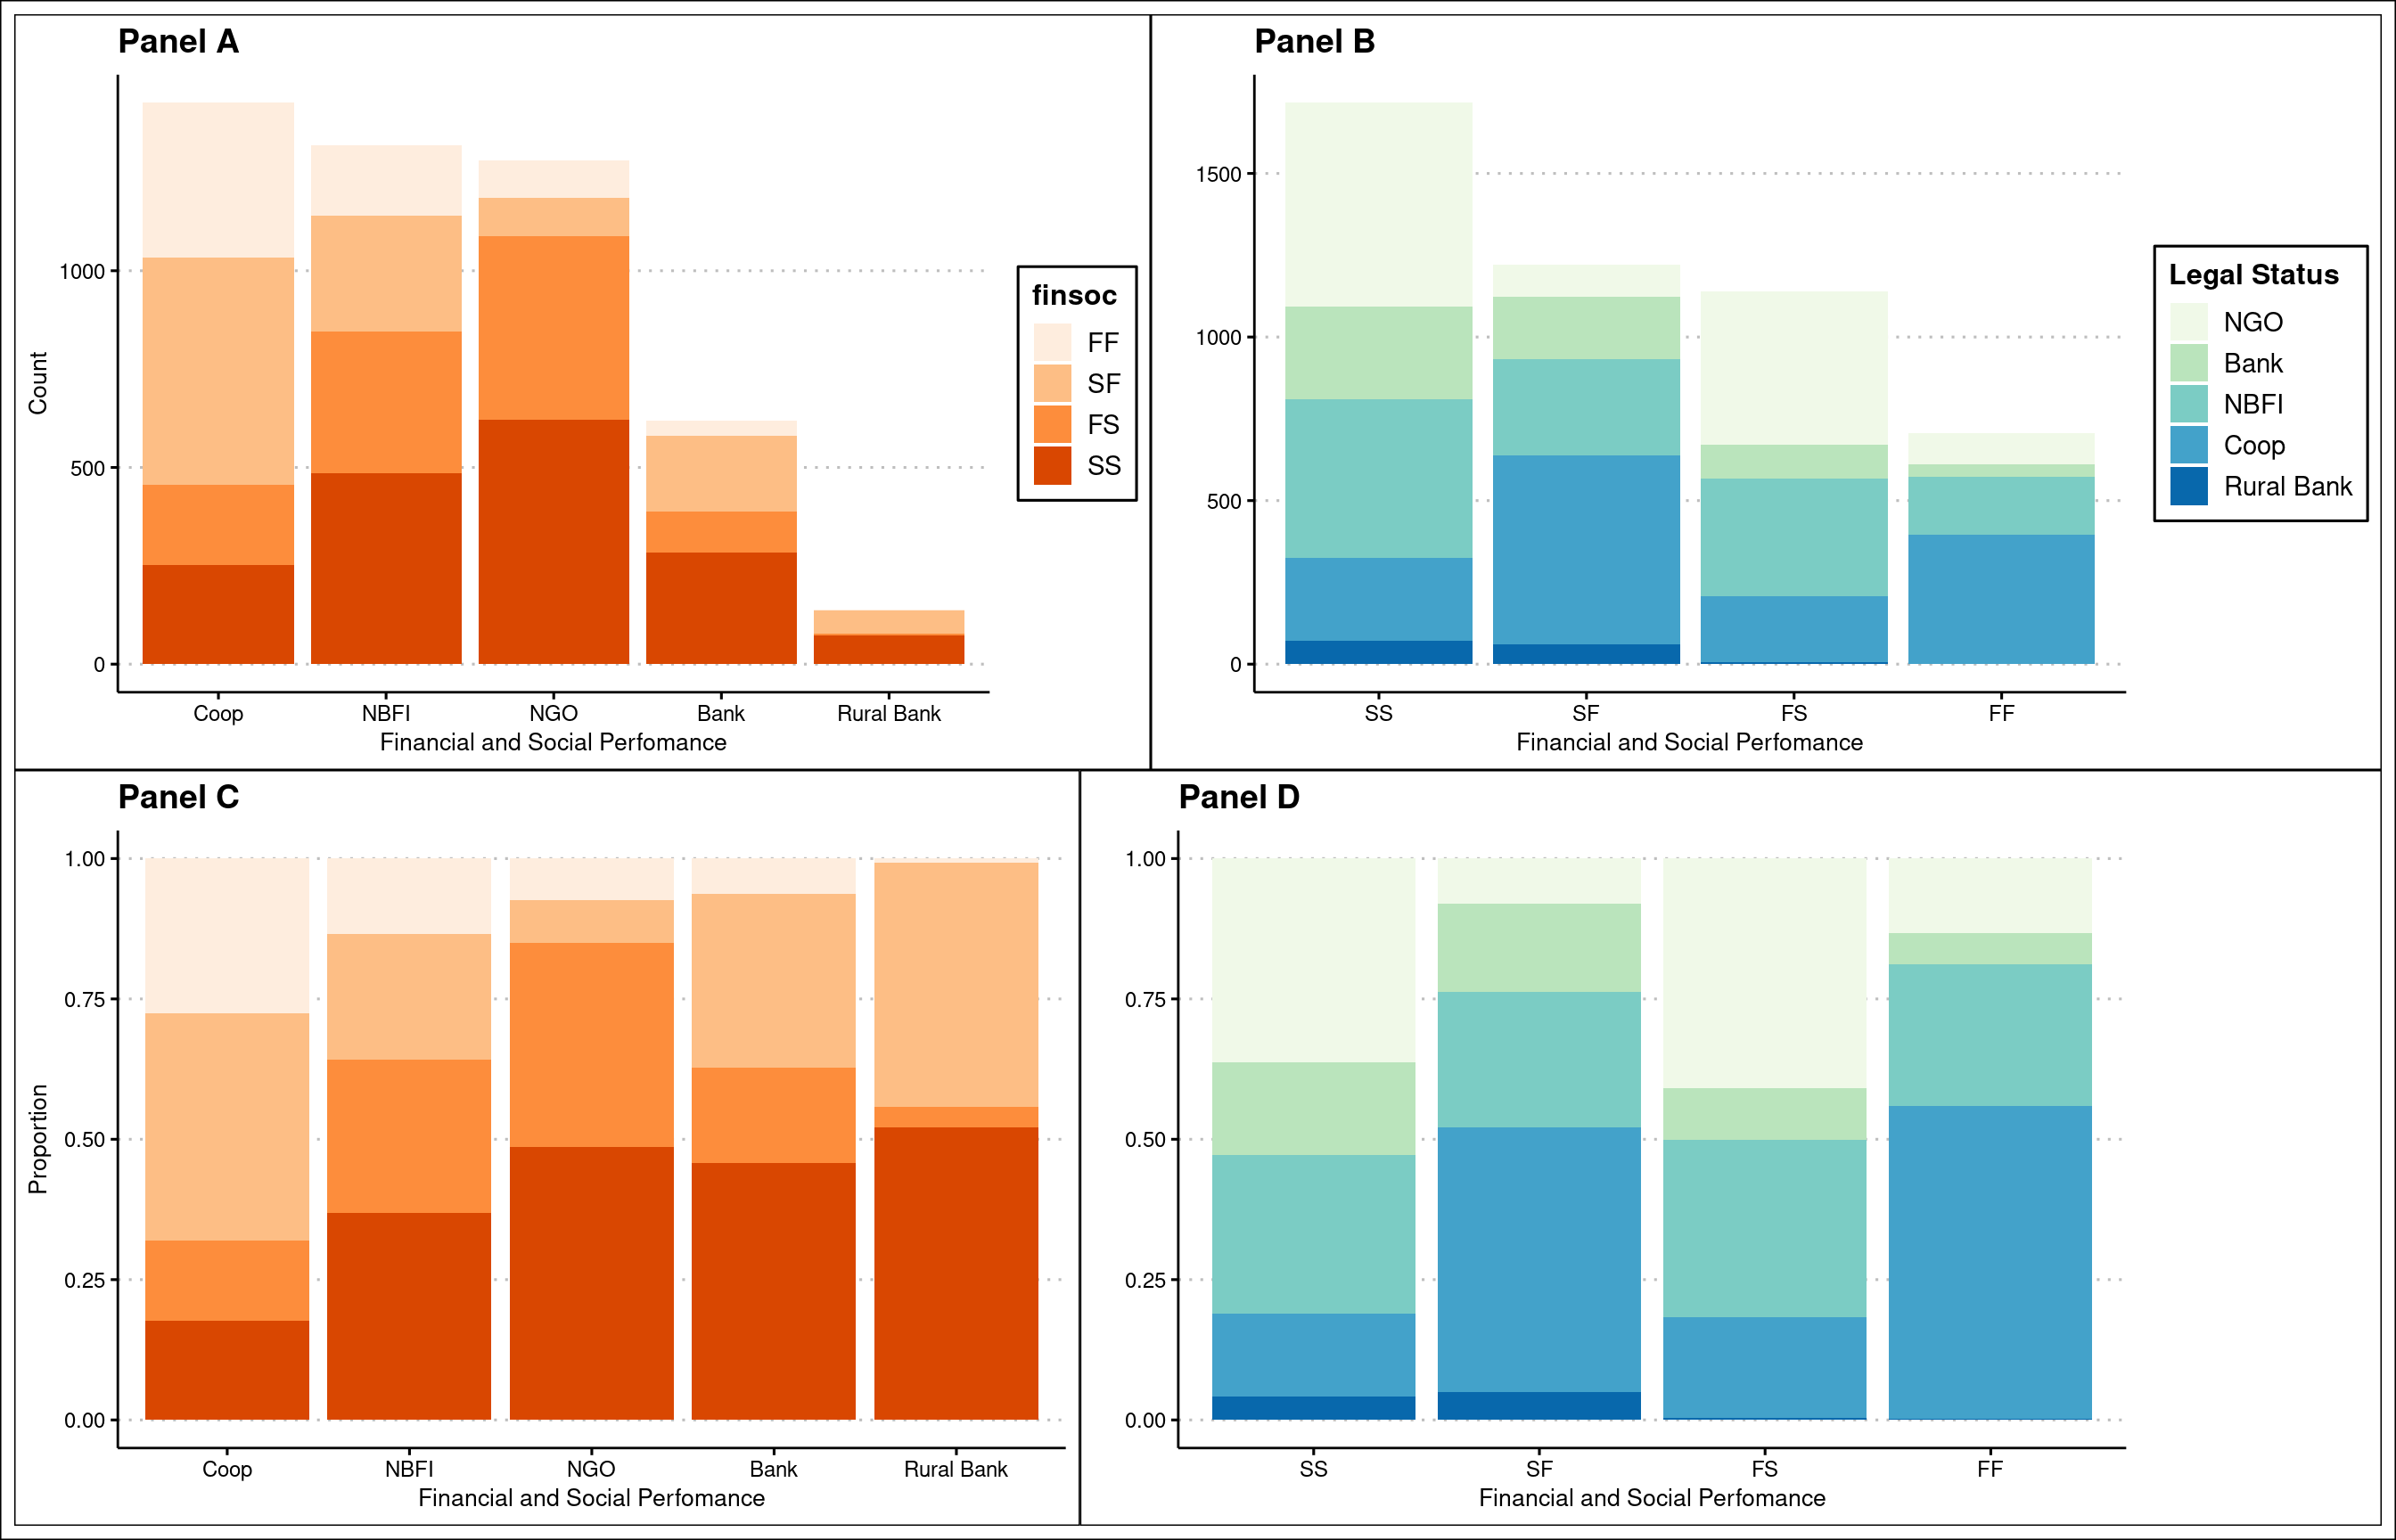
\includegraphics[width=8.8in]{_main_files/figure-latex/unnamed-chunk-146-1} 

}

\caption{Financial and Social Performance of MFIs in Africa}\label{fig:unnamed-chunk-146}
\end{figure}
\end{landscape}

\begin{landscape}

\begin{figure}

{\centering 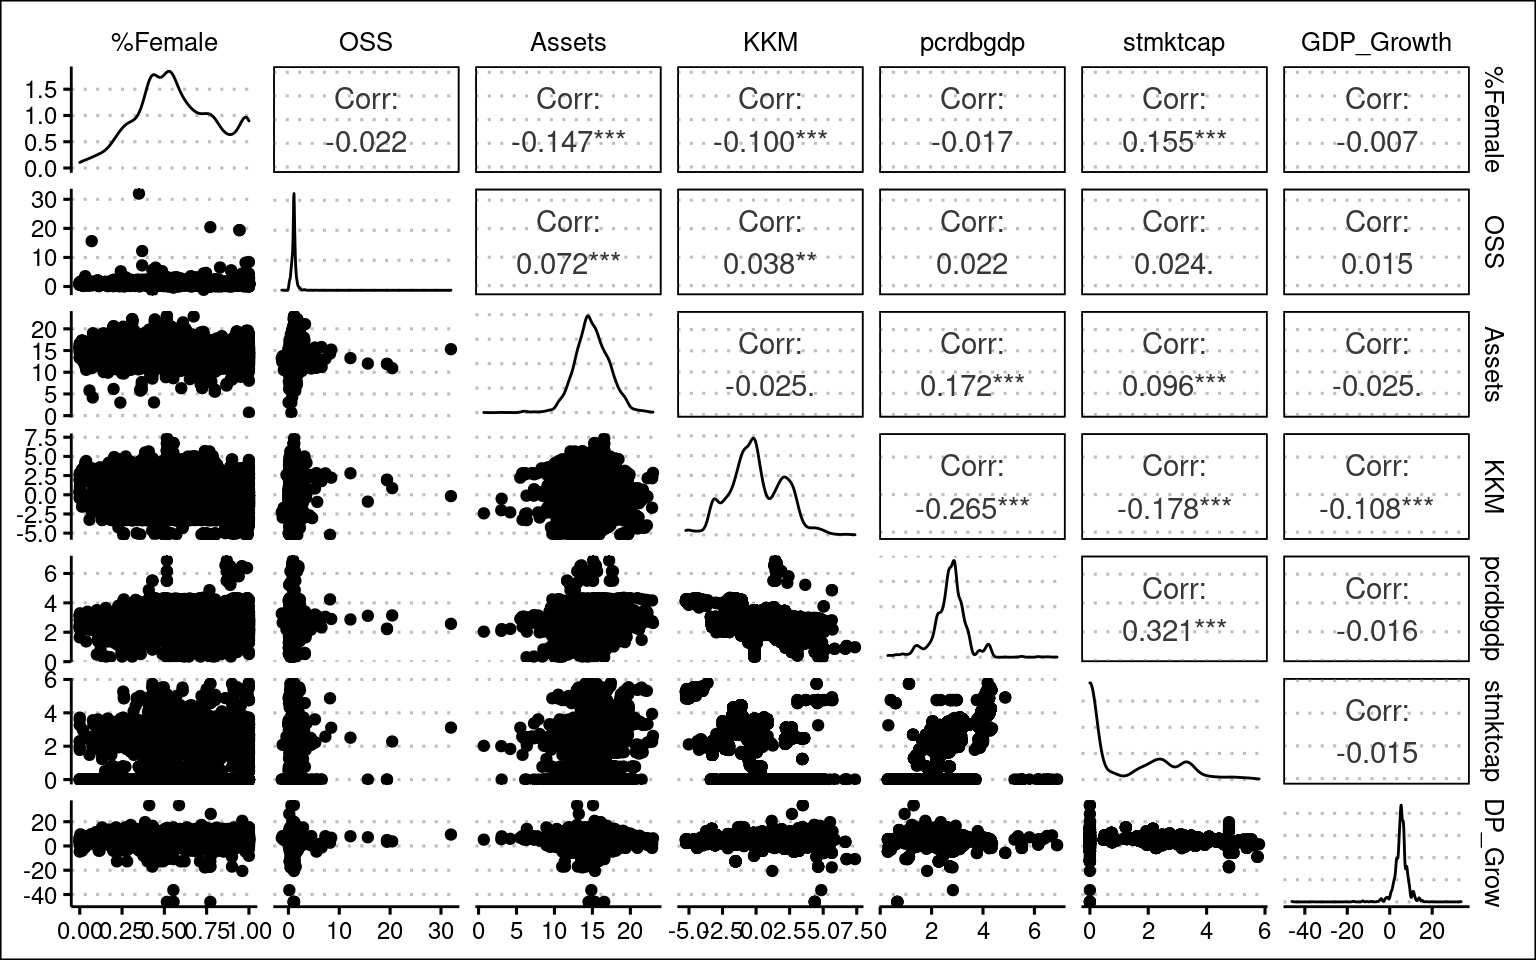
\includegraphics[width=8.8in]{_main_files/figure-latex/unnamed-chunk-151-1} 

}

\caption{Correlation between Independent Variables}\label{fig:unnamed-chunk-151}
\end{figure}

\end{landscape}

\begin{landscape}

\begin{figure}

{\centering 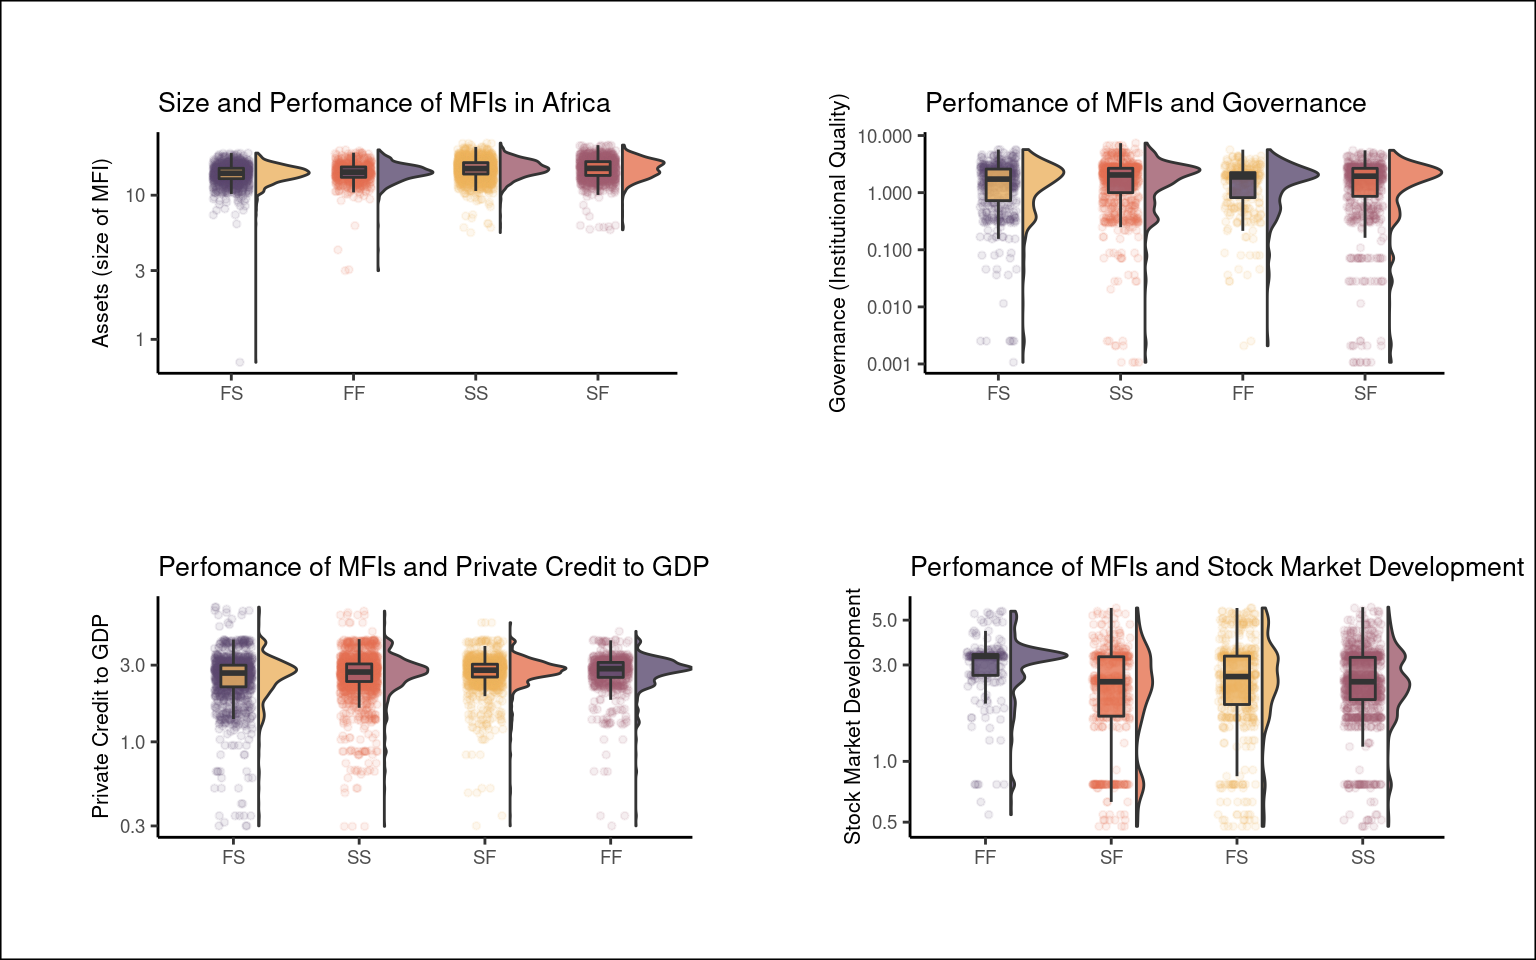
\includegraphics[width=8.8in]{_main_files/figure-latex/unnamed-chunk-152-1} 

}

\caption{Financial and Social Performance of MFIs by Size, Governance and Capital Mrkets Development}\label{fig:unnamed-chunk-152}
\end{figure}
\end{landscape}

\begin{landscape}
\begin{table}

\caption{\label{tab:unnamed-chunk-153}Summary statistics for continous numeric variables}
\centering
\fontsize{9}{11}\selectfont
\begin{tabu} to \linewidth {>{\raggedright}X>{\raggedleft}X>{\raggedleft}X>{\raggedleft}X>{\raggedleft}X>{\raggedleft}X>{\raggedleft}X>{\raggedleft}X}
\toprule
Variable & Mean & SD & Min & Q1 & Median & Q3 & Max\\
\midrule
percent\_of\_female\_borrowers & 0.5689 & 0.2366 & 0.0000 & 0.4206 & 0.5500 & 0.7478 & 1.000\\
operational\_self\_sufficiency & 1.0883 & 0.8642 & -1.3085 & 0.8376 & 1.0534 & 1.2358 & 31.964\\
assets & 14.9461 & 2.2619 & 0.6931 & 13.5399 & 14.8577 & 16.4162 & 22.979\\
kkm & 0.0026 & 2.0064 & -5.2332 & -1.3041 & -0.1137 & 1.6279 & 7.369\\
pcrdbgdp & 2.7194 & 0.6852 & 0.2981 & 2.3864 & 2.7584 & 3.0522 & 6.881\\
\addlinespace
stmktcap & 1.1410 & 1.4732 & 0.0000 & 0.0000 & 0.0000 & 2.4280 & 5.797\\
gdp\_growth\_annual & 5.3105 & 3.5905 & -46.0821 & 4.0000 & 5.4205 & 6.7233 & 33.629\\
donations & 88664.2095 & 315362.3616 & 1.0000 & 1.0000 & 3339.0000 & 60967.5000 & 10422018.000\\
donations\_assets\_ratio & 0.0435 & 0.1472 & -0.0033 & 0.0000 & 0.0008 & 0.0189 & 2.598\\
\bottomrule
\multicolumn{8}{l}{\rule{0pt}{1em}\textit{Source: }}\\
\multicolumn{8}{l}{\rule{0pt}{1em}Authors' construction from MIX data}\\
\end{tabu}
\end{table}

\end{landscape}

\hypertarget{results-of-the-regression-model-1}{%
\subsection{Results of the Regression Model}\label{results-of-the-regression-model-1}}

The results of the regression model are in Tables 8 through 10. Given that we have an unbalanced dataset, we run the regressions separately for the entire data (Table 6.8), for MFIs with three or more years of data (Table 6.9), and those with 5 or more years of data (Table 6.10). Overall, the significant drivers of achieving the dual objectives are age, size, stock market capitalization to GDP, private credit to GDP, institutional quality, legal tradition, and MFI legal status. The GDP growth rate is not a significant driver of the extent which MFIs meet both financial and social objectives. The latter two regressions form a robustness check. We discuss each of the variables basing them on Table 6.8 but referring to Tables 9 and 10 for comparison.

\hypertarget{age-1}{%
\subsubsection{Age}\label{age-1}}

\noindent Age is a categorical variable. New MFIs (that have existed for 0 - 4 years) are the base outcome. The results show that relative to new MFIs, young MFIs (4 -8 years) are less likely to succeed financially and fail socially than failing in both objectives. Put another way; young MFIs are more likely to experience both financial and social failure than they are to succeed financially and fail socially relative to new MFIs. Similarly, compared to new MFIs, young MFIs are less likely to fail financially and succeed in meeting their social goals than failing to meet the twin objectives. However, young MFIs are more likely than new MFIs to meet their financial and social goals than to fail in the dual mission. The results imply that young MFIs are more prone to financial and social failure than new MFIs. In other words, compared to new MFIs, young MFIs are more likely to fail to achieve both financial and social goals than they are to achieve social goals and to fail financially and vice versa, and succeeding both financially and socially. However, these relationships are not significant. Age is important given that newer MFIs have fewer resources and hence more reliant on donations which are also uncertain \autocite{armendariz2013subsidy,d2013unsubsidized}. Also, newer smaller firms have difficulties accessing finance \autocite{beck2008finance}. Thus, age makes newer MFIs more prone to financial and social failure and more prone to mission drift than established MFIs \autocite{d2017ngos}.

\begin{table}

\caption{\label{tab:unnamed-chunk-154}MFI Age and Achievement of Dual Objectives}
\centering
\begin{tabu} to \linewidth {>{\raggedright}X>{\raggedleft}X>{\raggedleft}X>{\raggedleft}X>{\raggedleft}X}
\toprule
  & FF & SF & FS & SS\\
\midrule
New & 0.1450 & 0.2400 & 0.3125 & 0.3025\\
Young & 0.1445 & 0.2217 & 0.2812 & 0.3525\\
Mature & 0.1501 & 0.2764 & 0.1857 & 0.3878\\
\bottomrule
\multicolumn{5}{l}{\rule{0pt}{1em}\textit{Source: }}\\
\multicolumn{5}{l}{\rule{0pt}{1em}Authors' construction from MIX data}\\
\end{tabu}
\end{table}

On the other hand, the results show that relative to new MFIs, mature MFIs are significantly less likely to succeed financially and fail socially than fail to meet the dual objectives. Similarly, mature MFIs are considerably less likely than new MFIs to fail financially while meeting their social goals than they are to meet both their goals. Both these results are significant. Also, the regression results show that relative to new MFIs, mature MFIs are less likely to meet the dual objectives than they are to fail in their twin mission. The latter result is not significant. These results illustrate that mature MFIs are more prone to failing in their twin mission than new MFIs. The results imply that as MFIs mature, they are less prone to mission drift. The observation holds, given that in the regression, older MFIs are more likely to fail to achieve both financial and social objectives than succeed in one and fail in the other or succeed in both financial and social goals, compared to new MFIs.

Indeed, Table 6.6 shows a higher proportion of mature MFIs fail to attain both objectives compared to new and young MFIs. although the difference is marginal. Likewise, a higher proportion of mature MFIs tend to succeed financially while failing socially, although, in the regression, the result is not significant. Financial success coupled with social failure implies mission drift and is detrimental to financial inclusion. Hence, these results suggest that mature MFIs are more prone to mission drift when they convert to the commercial model. Lastly, although the result is not significant in the regression, the Table 6.shows that mature MFIs that succeed financially also tend to succeed socially than do younger MFIs. \footnote{Note that the interpretation of Table 6.6 differs from the interpretation of the regression. The regression examines the relative likelihood. For instance, how likely are mature MFIs, as compared to new MFIs, to succeed in both objectives than fail in both objectives. The Table 6.gives absolute values.}

As noted, the results imply that mature MFIs are less prone to mission drift where success in one dimension (say, financial) accompanies failure in the other dimension (say social), and vice versa. However, when mature MFIs succeed financially, they also tend to fare equally well socially. The result could suggest that mature MFIs have a more extensive asset base to draw from, making them able to reach out to the financially excluded with less dependence on donations and subsidies. The larger asset base also means that larger MFIs have established their presence through marketing campaigns and technology such that they have a more extensive client base in diverse geographic locations \autocite{jia2016commercialization}. In this case, it is much easier for mature MFIs to attain their social goals, given their greater market share that would allow them to operate even in remote areas with or without donors and state support. Newer MFIs on the other hand, have to legitimize their activities by ensuring that they meet their social goals. Hence, even though mature MFIs receive more donations on aggregate, the relative share of donations is lower than that of newer MFIs.

\hypertarget{size}{%
\subsubsection{Size}\label{size}}

As noted, age and size move together. Mature MFIs have more assets on average than younger MFIs. The regression output shows that larger MFIs are significantly more likely to succeed financially while failing socially than they are to fail in both objectives. Specifically, suppose the asset base (the proxy for size) of an MFI rises by one unit. In that case, the MFI is 1.241102 times more likely to fall into the group that succeeds financially and fails socially than to be in the group that fails to meet the dual objectives.

On the contrary, larger MFIs are marginally less likely to fail in meeting their financial goals while succeeding socially. Again, a unit increase in size results in 0.9685066 likelihood of falling into the group of MFIs that fail financially while succeeding socially. With the odds almost equal to one, it appears size is not as crucial in determining whether an MFI fails financially and succeeds socially. Indeed, this outcome is not statistically significant. However, larger MFIs are significantly more likely to meet their dual goals than to fail in both. In this case, a unit increase in MFI size corresponds to 1.192438 odds of achieving both objectives relative to failing in both goals \footnote{We exponentiate the coefficients to get the odds. Odds greater than one indicate greater likelihood. Odds less than one indicate less likelihood, while one indicates equal likelihood.}.

The results highlight that size is a critical ingredient in determining whether or not MFIs meet their dual objectives. Larger MFIs have a greater likelihood of achieving both objectives and meeting their financial goals while failing socially. This means that while the size of an MFI is a crucial factor in meeting social goals, it is a factor of greater importance in meeting financial objectives. The results also imply that larger MFIs that meet their financial objectives are in a better position to also meet their social goals. Hence, meeting financial goals is a prerequisite for meeting social goals for larger MFIs relative to smaller, younger MFIs. Larger MFIs use their asset base to generate financial resources that they use to expand outreach to the financially excluded, consistent with the ``mission expansion'' view \autocite{mersland2010microfinance}. For relatively small MFIs, donations and subsidies form a higher proportion of assets and hence are not as reliant on making financial returns to fund their operations.

\hypertarget{capital-markets-development}{%
\subsubsection{Capital markets development}\label{capital-markets-development}}

This section covers both the stock market development and the debt market development. The regression shows that across all classes, MFIs located in countries with better stock market development are less likely to meet the dual objectives than failing in both goals. Going by the coefficients, a unit increase in stock market capitalisation results in 0.8633 times as likely to meet the twin objectives than to fail in both. Similarly, MFIs located in these countries are less likely to meet their financial goals and fail socially. In this case, a unit increase in stock market development corresponds with a 0.8573 odds of being in the category of MFIs that succeed financially while failing socially than in the class that fails to meet both objectives. Likewise, higher stock market development connotes a higher probability of an MFI succeeding financially while failing in their social mandate than failing in both goals. Here, a unit increase in stock market capitalisation corresponds to 0.8228 odds.

Debt market development, whose proxy is the ratio of private credit to GDP follows a similar pattern. A higher level of debt market development corresponds to higher odds of succeeding financially while failing socially instead of failing in both objectives. The result is not significant, though. However, a higher level of debt market development lowers the odds of an MFI failing financially and succeeding socially. Also, higher debt market development reduces the odds of an MFI succeeding in both objectives versus failing in both. The corresponding odds are 0.7757 and 0.8633, respectively.

Indeed in countries where stock markets are well-developed, the mainstream financial system, including the debt market, is also likely well established, meaning that people can easily access finance. Research shows that a well developed debt market is a precursor to developing a stock market \autocite{nguyen2012determinants,tsaurai2018determinants}. Under these conditions, the demand for microfinance is low, meaning that it is hard for MFIs to realise their objectives. The few MFIs that exist in these conditions are more likely to serve a small, underprivileged class, meaning that the possibility of achieving their financial goals are minimal. They, however, almost always meet their social goals.

\hypertarget{governance-institutional-quality-kkm}{%
\subsubsection{Governance/ Institutional quality (KKM)}\label{governance-institutional-quality-kkm}}

Institutional quality goes together with better financial sector development \autocite{allen2014african}. The regressions results show that a unit increase in institutional quality corresponds with higher odds of succeeding financially while failing socially. The odds are 1.1219. With odds of 0.9231, when institutional quality goes up by a unit, there is a lower chance of an MFI failing financially and succeeding socially than failing in both goals. These two results are statistically significant. Finally, a unit increase in institutional quality lowers the chances of an MFI meeting both objectives compared to failing in both objectives with odd of 1.0305. The result is, however, insignificant. As is the case for financial sector development, the populace in countries with better quality institutions is more likely to have access to the mainstream financial system, making social goals harder for MFIs given the low demand for microfinance \autocite{butkiewicz2006institutional}. Given a low demand for microfinance, it is also harder for MFIs to succeed financially.

\hypertarget{legal-tradition-1}{%
\subsubsection{Legal Tradition}\label{legal-tradition-1}}

The common law legal tradition is the base outcome for this variable. The results show that, relative to MFIs in common law countries, MFIs in civil law countries are less likely to succeed financially while failing socially than fail in both objectives. The odds are 0.2753. Similarly, MFIs in civil law countries are less likely than MFIs in common law countries to fail financially while succeeding socially than they are to fail in both objectives with an odds of 0.386. Also, MFIs operating in civil law countries are less likely than those in common law countries to succeed in both objectives than to fail in both objectives. The odds are 0.2982. The odds are strikingly low, showing the high likelihood of MFIs in civil law countries to fail in both financial and social goals compared to those in common law countries.

For MFIs in other legal traditions (neither common law nor civil law), the results are similar to those for civil law countries. The odds are lower (at 0.3679) that an MFI in a country with other legal traditions, compared to common law countries, will succeed financially and fail socially instead of failing in both objectives. The odds for failing financially while succeeding socially and succeeding in both goals are 0.5337 and 0.3946, respectively. Table 6.7 confirms that indeed, MFIs in civil law countries and other legal traditions are more likely to fail to meet both objectives than those in common law countries. Also, MFIs in common law countries have the highest instance of succeeding socially. Civil law and other legal tradition countries have a lower capital markets development level than common law countries \autocite{schnyder2018twenty,kaidi2019financial}.

Consequently, we would expect that MFIs find it easier to meet social goals in civil law countries. These results could point to poor reception of financial services in these countries \autocite{la2013law}. Additionally, lack of a supportive legal framework, inadequate financial and physical infrastructure could also make it difficult for MFIs to meet their social mandate even when the demand for microfinance is potentially high.

\begin{table}

\caption{\label{tab:unnamed-chunk-155}Legal Traditions and Achievement of Dual Objectives}
\centering
\begin{tabu} to \linewidth {>{\raggedright}X>{\raggedleft}X>{\raggedleft}X>{\raggedleft}X>{\raggedleft}X}
\toprule
  & FF & SF & FS & SS\\
\midrule
Common & 0.0671 & 0.2270 & 0.2589 & 0.4470\\
Civil & 0.2131 & 0.2731 & 0.2147 & 0.2991\\
Other & 0.1761 & 0.2756 & 0.2415 & 0.3068\\
\bottomrule
\multicolumn{5}{l}{\rule{0pt}{1em}\textit{Source: }}\\
\multicolumn{5}{l}{\rule{0pt}{1em}Authors' construction from MIX data}\\
\end{tabu}
\end{table}

\hypertarget{mfi-legal-status}{%
\subsubsection{MFI legal status}\label{mfi-legal-status}}

For legal status, the NGO model is the base outcome. Compared to NGOs, commercial banks are more likely to succeed financially while failing socially than they are to fail in both objectives. The results show that microfinance's commercial banking model is likely to put profits before outreach to the financially excluded. Similarly, commercial banks are less likely than NGOs to fail financially while succeeding socially than failing in both objectives. The result may highlight that for commercial banks to succeed socially, they have to be financially self-sustainable, without which they tend to fail in both objectives. Likewise, relative to NGOs, commercial banks are less likely to achieve both financial and social goals than fail in both goals. Again this shows the importance of financial success in determining the attainment of social objectives by commercial banks compared to NGOs.

The other MFI legal forms, that is, NBFIs, cooperatives, and rural banks show a pattern similar to that of commercial banks. Overall, the results confirm the results of exploratory data analysis that show that NGOs are less prone to social failure than the commercial forms of MFIs \autocite{jia2016commercialization,mia2017mission}. The result confirms the welfare school's concerns that the transformation of MFIs is likely to cause mission drift \autocite{d2017ngos}. Also, it implies that for commercial MFIs to prioritize social goals, they should first realize financial success which may be hard to come by unless with some form of support from the state and donors, at least in the initial stages of transformation.

\newpage

\begin{table}[!htbp] \centering 
  \caption{Regression Results - Multinomial Logit Model- Full Data} 
  \label{} 
\footnotesize 
\begin{tabular}{@{\extracolsep{5pt}}lccc} 
\\[-1.8ex]\hline 
\hline \\[-1.8ex] 
 & \multicolumn{3}{c}{\textit{Dependent variable:}} \\ 
\cline{2-4} 
\\[-1.8ex] & SF & FS & SS \\ 
\\[-1.8ex] & (1) & (2) & (3)\\ 
\hline \\[-1.8ex] 
 ageYoung & $-$0.039 & $-$0.095 & 0.060 \\ 
  & (0.152) & (0.151) & (0.148) \\ 
  & & & \\ 
 ageMature & $-$0.233$^{*}$ & $-$0.483$^{***}$ & $-$0.191 \\ 
  & (0.138) & (0.141) & (0.136) \\ 
  & & & \\ 
 assets & 0.216$^{***}$ & $-$0.032 & 0.176$^{***}$ \\ 
  & (0.028) & (0.029) & (0.028) \\ 
  & & & \\ 
 stmktcap & $-$0.195$^{***}$ & $-$0.154$^{***}$ & $-$0.147$^{***}$ \\ 
  & (0.054) & (0.054) & (0.050) \\ 
  & & & \\ 
 pcrdbgdp & 0.060 & $-$0.254$^{***}$ & $-$0.147 \\ 
  & (0.091) & (0.096) & (0.091) \\ 
  & & & \\ 
 kkm & 0.115$^{***}$ & $-$0.080$^{***}$ & 0.030 \\ 
  & (0.029) & (0.030) & (0.028) \\ 
  & & & \\ 
 gdp\_growth\_annual & 0.026 & $-$0.019 & $-$0.006 \\ 
  & (0.016) & (0.015) & (0.015) \\ 
  & & & \\ 
 legal\_traditionCivil & $-$1.290$^{***}$ & $-$0.952$^{***}$ & $-$1.207$^{***}$ \\ 
  & (0.200) & (0.194) & (0.184) \\ 
  & & & \\ 
 legal\_traditionOther & $-$1.005$^{***}$ & $-$0.628$^{***}$ & $-$0.930$^{***}$ \\ 
  & (0.182) & (0.181) & (0.172) \\ 
  & & & \\ 
 currentlegalstatusBank & 0.605$^{**}$ & $-$0.843$^{***}$ & $-$0.671$^{***}$ \\ 
  & (0.253) & (0.247) & (0.232) \\ 
  & & & \\ 
 currentlegalstatusNBFI & 0.002 & $-$1.035$^{***}$ & $-$1.241$^{***}$ \\ 
  & (0.188) & (0.165) & (0.159) \\ 
  & & & \\ 
 currentlegalstatusCoop & 0.508$^{***}$ & $-$2.288$^{***}$ & $-$2.155$^{***}$ \\ 
  & (0.173) & (0.159) & (0.151) \\ 
  & & & \\ 
 currentlegalstatusRural Bank & 3.638$^{***}$ & $-$0.826 & 1.702$^{*}$ \\ 
  & (1.024) & (1.106) & (1.017) \\ 
  & & & \\ 
 Constant & 1.853$^{***}$ & 8.566$^{***}$ & 4.337$^{***}$ \\ 
  & (0.552) & (0.504) & (0.512) \\ 
  & & & \\ 
\hline \\[-1.8ex] 
Year Effects & Yes & Yes & Yes \\ 
Data & Full & Full & Full \\ 
Akaike Inf. Crit. & 11,446.000 & 11,446.000 & 11,446.000 \\ 
\hline 
\hline \\[-1.8ex] 
\textit{Note:}  & \multicolumn{3}{r}{$^{*}$p$<$0.1; $^{**}$p$<$0.05; $^{***}$p$<$0.01} \\ 
\end{tabular} 
\end{table}

\newpage

\begin{table}[!htbp] \centering 
  \caption{Regression Results - Multinomial Logit Model- At Least 3 Years of Data} 
  \label{} 
\footnotesize 
\begin{tabular}{@{\extracolsep{5pt}}lccc} 
\\[-1.8ex]\hline 
\hline \\[-1.8ex] 
 & \multicolumn{3}{c}{\textit{Dependent variable:}} \\ 
\cline{2-4} 
\\[-1.8ex] & SF & FS & SS \\ 
\\[-1.8ex] & (1) & (2) & (3)\\ 
\hline \\[-1.8ex] 
 ageYoung & 0.061 & $-$0.163 & 0.132 \\ 
  & (0.168) & (0.161) & (0.160) \\ 
  & & & \\ 
 ageMature & $-$0.105 & $-$0.553$^{***}$ & $-$0.136 \\ 
  & (0.154) & (0.152) & (0.149) \\ 
  & & & \\ 
 assets & 0.232$^{***}$ & $-$0.046 & 0.172$^{***}$ \\ 
  & (0.031) & (0.031) & (0.030) \\ 
  & & & \\ 
 stmktcap & $-$0.161$^{***}$ & $-$0.172$^{***}$ & $-$0.154$^{***}$ \\ 
  & (0.057) & (0.057) & (0.053) \\ 
  & & & \\ 
 pcrdbgdp & 0.036 & $-$0.225$^{**}$ & $-$0.126 \\ 
  & (0.095) & (0.100) & (0.095) \\ 
  & & & \\ 
 kkm & 0.110$^{***}$ & $-$0.101$^{***}$ & 0.021 \\ 
  & (0.031) & (0.032) & (0.030) \\ 
  & & & \\ 
 gdp\_growth\_annual & 0.031$^{*}$ & $-$0.020 & $-$0.005 \\ 
  & (0.017) & (0.016) & (0.015) \\ 
  & & & \\ 
 legal\_traditionCivil & $-$1.153$^{***}$ & $-$0.930$^{***}$ & $-$1.190$^{***}$ \\ 
  & (0.211) & (0.203) & (0.192) \\ 
  & & & \\ 
 legal\_traditionOther & $-$0.892$^{***}$ & $-$0.654$^{***}$ & $-$0.937$^{***}$ \\ 
  & (0.193) & (0.191) & (0.181) \\ 
  & & & \\ 
 currentlegalstatusBank & 0.622$^{**}$ & $-$0.873$^{***}$ & $-$0.665$^{***}$ \\ 
  & (0.260) & (0.255) & (0.238) \\ 
  & & & \\ 
 currentlegalstatusNBFI & 0.044 & $-$0.952$^{***}$ & $-$1.244$^{***}$ \\ 
  & (0.193) & (0.170) & (0.165) \\ 
  & & & \\ 
 currentlegalstatusCoop & 0.397$^{**}$ & $-$2.177$^{***}$ & $-$2.047$^{***}$ \\ 
  & (0.179) & (0.166) & (0.156) \\ 
  & & & \\ 
 currentlegalstatusRural Bank & 20.220$^{***}$ & 15.030$^{***}$ & 18.120$^{***}$ \\ 
  & (0.276) & (0.484) & (0.267) \\ 
  & & & \\ 
 Constant & 3.146$^{***}$ & 10.410$^{***}$ & 5.944$^{***}$ \\ 
  & (0.581) & (0.535) & (0.536) \\ 
  & & & \\ 
\hline \\[-1.8ex] 
Year Effects & Yes & Yes & Yes \\ 
Data & At Least 3 Years & At Least 3 Years & At Least 3 Years \\ 
Akaike Inf. Crit. & 10,438.000 & 10,438.000 & 10,438.000 \\ 
\hline 
\hline \\[-1.8ex] 
\textit{Note:}  & \multicolumn{3}{r}{$^{*}$p$<$0.1; $^{**}$p$<$0.05; $^{***}$p$<$0.01} \\ 
\end{tabular} 
\end{table}

\newpage

\begin{table}[!htbp] \centering 
  \caption{Regression Results - Multinomial Logit Model, at Least 5 Years of Data} 
  \label{} 
\footnotesize 
\begin{tabular}{@{\extracolsep{5pt}}lccc} 
\\[-1.8ex]\hline 
\hline \\[-1.8ex] 
 & \multicolumn{3}{c}{\textit{Dependent variable:}} \\ 
\cline{2-4} 
\\[-1.8ex] & SF & FS & SS \\ 
\\[-1.8ex] & (1) & (2) & (3)\\ 
\hline \\[-1.8ex] 
 ageYoung & 0.720$^{***}$ & 0.043 & 0.642$^{***}$ \\ 
  & (0.216) & (0.188) & (0.193) \\ 
  & & & \\ 
 ageMature & 0.475$^{**}$ & $-$0.367$^{**}$ & 0.243 \\ 
  & (0.198) & (0.173) & (0.177) \\ 
  & & & \\ 
 assets & 0.352$^{***}$ & $-$0.135$^{***}$ & 0.254$^{***}$ \\ 
  & (0.040) & (0.042) & (0.038) \\ 
  & & & \\ 
 stmktcap & $-$0.170$^{**}$ & $-$0.219$^{***}$ & $-$0.185$^{***}$ \\ 
  & (0.068) & (0.067) & (0.062) \\ 
  & & & \\ 
 pcrdbgdp & $-$0.029 & $-$0.132 & $-$0.152 \\ 
  & (0.104) & (0.107) & (0.102) \\ 
  & & & \\ 
 kkm & 0.061$^{*}$ & $-$0.159$^{***}$ & $-$0.049 \\ 
  & (0.036) & (0.036) & (0.034) \\ 
  & & & \\ 
 gdp\_growth\_annual & 0.018 & $-$0.009 & $-$0.004 \\ 
  & (0.018) & (0.018) & (0.017) \\ 
  & & & \\ 
 legal\_traditionCivil & $-$0.963$^{***}$ & $-$0.915$^{***}$ & $-$1.136$^{***}$ \\ 
  & (0.234) & (0.222) & (0.210) \\ 
  & & & \\ 
 legal\_traditionOther & $-$0.574$^{**}$ & $-$0.873$^{***}$ & $-$0.755$^{***}$ \\ 
  & (0.226) & (0.223) & (0.208) \\ 
  & & & \\ 
 currentlegalstatusBank & $-$0.008 & $-$0.536$^{*}$ & $-$1.101$^{***}$ \\ 
  & (0.289) & (0.283) & (0.263) \\ 
  & & & \\ 
 currentlegalstatusNBFI & $-$0.020 & $-$0.817$^{***}$ & $-$1.356$^{***}$ \\ 
  & (0.208) & (0.184) & (0.178) \\ 
  & & & \\ 
 currentlegalstatusCoop & 0.241 & $-$2.058$^{***}$ & $-$1.959$^{***}$ \\ 
  & (0.199) & (0.187) & (0.175) \\ 
  & & & \\ 
 currentlegalstatusRural Bank & 20.350$^{***}$ & $-$4.881$^{***}$ & 17.790$^{***}$ \\ 
  & (0.171) & (0.000) & (0.171) \\ 
  & & & \\ 
 Constant & 0.856 & 10.880$^{***}$ & 4.188$^{***}$ \\ 
  & (0.698) & (0.672) & (0.645) \\ 
  & & & \\ 
\hline \\[-1.8ex] 
Year Effects & Yes & Yes & Yes \\ 
Data & >at Least 5 Years & at Least 5 Years & at Least 5 Years \\ 
Akaike Inf. Crit. & 8,252.000 & 8,252.000 & 8,252.000 \\ 
\hline 
\hline \\[-1.8ex] 
\textit{Note:}  & \multicolumn{3}{r}{$^{*}$p$<$0.1; $^{**}$p$<$0.05; $^{***}$p$<$0.01} \\ 
\end{tabular} 
\end{table}

\newpage

\hypertarget{overall-model-fit-confusion-matrix}{%
\subsection{Overall Model Fit: Confusion Matrix}\label{overall-model-fit-confusion-matrix}}

This section uses the regression model in Table 6.8 to generate a confusion matrix that shows how well the model predicts that an MFI will fall into one of the four financial vis-a-vis social performance classes. The results are in Table 6.11 and Table 6.12. In Table 6.11, while the model has low accuracy and sensitivity, it has a substantial specificity of about 80\%. The results mean that the model can accurately predict that an MFI will not fall into a given category given that it does not fall into that category. However, the model is not significantly more accurate than guessing the most likely outcome. In this case, an MFI succeeds financially and socially, with an accuracy of 46.9\% against a no-information rate of 52.9\%. Table 6.12 shows that, for instance, the model accurately predicts that 141 MFIs would fail in attaining both financial and social goals. However, 706 fail to meet both objectives \footnote{This Figure 6.is the sum of the first row.}. This presents a poor prediction accuracy of 19.97\%. However, the model does well to predict MFIs that succeed in both objectives, getting it right 1202 instances. In this case, the overall accuracy is high at 70\%. The second (SF) and third categories (FS) accuracy are 41\% and 34.8\%, respectively. The model quickly picks out MFIs that succeed in both objectives better than it does the other categories.

\begin{table}

\caption{\label{tab:unnamed-chunk-160}Confusion Matrix and Statistics for the Multinomial Logit Model}
\centering
\begin{tabu} to \linewidth {>{\raggedright}X>{\raggedleft}X>{\raggedleft}X>{\raggedleft}X>{\raggedleft}X}
\toprule
  & FF & SF & FS & FF\\
\midrule
Accuracy & 0.4690 & 0.469 & 0.4690 & 0.469\\
NoInformationRate & 0.5290 & 0.529 & 0.5290 & 0.529\\
Kappa & 0.2430 & 0.243 & 0.2430 & 0.243\\
sensitivity & 0.4040 & 0.466 & 0.4859 & 0.475\\
specificity & 0.8725 & 0.806 & 0.8130 & 0.772\\
\addlinespace
PosPredValue & 0.1997 & 0.414 & 0.3480 & 0.700\\
NegPredValue & 0.9490 & 0.837 & 0.8850 & 0.566\\
Prevalence & 0.0730 & 0.227 & 0.1704 & 0.529\\
DetectionRate & 0.0295 & 0.106 & 0.0828 & 0.251\\
DetectionPrevalence & 0.1476 & 0.256 & 0.2380 & 0.359\\
\addlinespace
BalancedAccuracy & 0.6383 & 0.636 & 0.6494 & 0.623\\
\bottomrule
\multicolumn{5}{l}{\rule{0pt}{1em}\textit{Source: }}\\
\multicolumn{5}{l}{\rule{0pt}{1em}Authors' construction}\\
\multicolumn{5}{l}{\rule{0pt}{1em}\textit{Notes: }}\\
\multicolumn{5}{l}{\rule{0pt}{1em}\textsuperscript{1} Accuracy > NoInformationRate is significant at 1\% confidence level, p = 0.0000}\\
\end{tabu}
\end{table}

\begin{table}

\caption{\label{tab:unnamed-chunk-161}Confusion Matrix Table for the Multinomial Logit Model}
\centering
\begin{tabu} to \linewidth {>{\raggedright}X>{\raggedleft}X>{\raggedleft}X>{\raggedleft}X>{\raggedleft}X}
\toprule
  & FF & SF & FS & SS\\
\midrule
FF & 141 & 242 & 99 & 224\\
SF & 90 & 506 & 77 & 549\\
FS & 63 & 122 & 396 & 557\\
SS & 55 & 216 & 243 & 1202\\
\bottomrule
\multicolumn{5}{l}{\rule{0pt}{1em}\textit{Source: }}\\
\multicolumn{5}{l}{\rule{0pt}{1em}Authors' construction}\\
\end{tabu}
\end{table}

\hypertarget{regression-diagnostics-1}{%
\subsection{Regression Diagnostics}\label{regression-diagnostics-1}}

In this section, we do robustness checks on the regression for extreme values, multicollinearity and linearity. Note that we base the checks on the model in Table 6.8 that utilize the entire dataset.

\hypertarget{extreme-values-1}{%
\subsubsection{Extreme Values}\label{extreme-values-1}}

In the regression model, we winsorize the data by removing the top and bottom 10\% and re-run the analysis. The results of the regression are in Table 6.13 below. Extreme values do not affect the results do not change except for the expected changes in the coefficients.

\begin{table}[!htbp] \centering 
  \caption{Regression Results - Multinomial Logit Model, Winsorized Data} 
  \label{} 
\footnotesize 
\begin{tabular}{@{\extracolsep{5pt}}lccc} 
\\[-1.8ex]\hline 
\hline \\[-1.8ex] 
 & \multicolumn{3}{c}{\textit{Dependent variable:}} \\ 
\cline{2-4} 
\\[-1.8ex] & SF & FS & SS \\ 
\\[-1.8ex] & (1) & (2) & (3)\\ 
\hline \\[-1.8ex] 
 ageYoung & $-$0.047 & $-$0.113 & 0.044 \\ 
  & (0.157) & (0.157) & (0.154) \\ 
  & & & \\ 
 ageMature & $-$0.285$^{**}$ & $-$0.377$^{**}$ & $-$0.111 \\ 
  & (0.143) & (0.148) & (0.142) \\ 
  & & & \\ 
 assets & 0.245$^{***}$ & $-$0.076$^{**}$ & 0.176$^{***}$ \\ 
  & (0.030) & (0.033) & (0.030) \\ 
  & & & \\ 
 stmktcap & $-$0.226$^{***}$ & $-$0.049 & $-$0.109$^{*}$ \\ 
  & (0.059) & (0.060) & (0.056) \\ 
  & & & \\ 
 pcrdbgdp & 0.119 & $-$0.613$^{***}$ & $-$0.237$^{*}$ \\ 
  & (0.130) & (0.131) & (0.126) \\ 
  & & & \\ 
 kkm & 0.118$^{***}$ & $-$0.131$^{***}$ & $-$0.002 \\ 
  & (0.031) & (0.033) & (0.031) \\ 
  & & & \\ 
 gdp\_growth\_annual & 0.040$^{*}$ & $-$0.018 & 0.035 \\ 
  & (0.024) & (0.025) & (0.024) \\ 
  & & & \\ 
 legal\_traditionCivil & $-$1.277$^{***}$ & $-$0.604$^{***}$ & $-$1.042$^{***}$ \\ 
  & (0.213) & (0.208) & (0.197) \\ 
  & & & \\ 
 legal\_traditionOther & $-$0.991$^{***}$ & $-$0.427$^{**}$ & $-$1.003$^{***}$ \\ 
  & (0.188) & (0.191) & (0.181) \\ 
  & & & \\ 
 currentlegalstatusBank & 0.486$^{*}$ & $-$0.717$^{***}$ & $-$0.682$^{***}$ \\ 
  & (0.257) & (0.253) & (0.237) \\ 
  & & & \\ 
 currentlegalstatusNBFI & $-$0.081 & $-$1.022$^{***}$ & $-$1.234$^{***}$ \\ 
  & (0.192) & (0.170) & (0.164) \\ 
  & & & \\ 
 currentlegalstatusCoop & 0.483$^{***}$ & $-$2.415$^{***}$ & $-$2.105$^{***}$ \\ 
  & (0.177) & (0.166) & (0.156) \\ 
  & & & \\ 
 currentlegalstatusRural Bank & 3.658$^{***}$ & $-$0.905 & 1.627 \\ 
  & (1.029) & (1.110) & (1.022) \\ 
  & & & \\ 
 Constant & 1.029$^{*}$ & 9.384$^{***}$ & 3.956$^{***}$ \\ 
  & (0.616) & (0.591) & (0.575) \\ 
  & & & \\ 
\hline \\[-1.8ex] 
Year Effects & Yes & Yes & Yes \\ 
Data & Full Data & Full Data & Full Data \\ 
Akaike Inf. Crit. & 10,657.000 & 10,657.000 & 10,657.000 \\ 
\hline 
\hline \\[-1.8ex] 
\textit{Note:}  & \multicolumn{3}{r}{$^{*}$p$<$0.1; $^{**}$p$<$0.05; $^{***}$p$<$0.01} \\ 
\end{tabular} 
\end{table}

\hypertarget{multicollinearity-1}{%
\subsubsection{multicollinearity}\label{multicollinearity-1}}

This section checks for multi-collinearity among the independent variables by generating the variance inflation factors (VIFs). In this case, the mainstream variables do not have exceptional variance inflation. The VIFs are in Table 6.14. However, the inclusion of year effects is vital in the regressions, given their panel structure.

\begin{table}

\caption{\label{tab:unnamed-chunk-164}Variance Inflation Factors for Logit Model}
\centering
\begin{tabu} to \linewidth {>{\raggedright}X>{\raggedleft}X>{\raggedleft}X>{\raggedleft}X}
\toprule
  & GVIF & Df & GVIF\textasciicircum{}(1/(2*Df))\\
\midrule
age & 1.437 & 2 & 1.095\\
assets & 1.626 & 1 & 1.275\\
stmktcap & 2.533 & 1 & 1.591\\
pcrdbgdp & 1.660 & 1 & 1.288\\
kkm & 1.322 & 1 & 1.150\\
\addlinespace
gdp\_growth\_annual & 1.154 & 1 & 1.074\\
legal\_tradition & 3.004 & 2 & 1.317\\
currentlegalstatus & 2.244 & 4 & 1.106\\
factor(year) & 1.619 & 20 & 1.012\\
\bottomrule
\multicolumn{4}{l}{\rule{0pt}{1em}\textit{Source: }}\\
\multicolumn{4}{l}{\rule{0pt}{1em}Authors' construction}\\
\end{tabu}
\end{table}

\hypertarget{conclusion-3}{%
\subsection{Conclusion}\label{conclusion-3}}

This article examines the extent to which MFIs in Africa achieve their dual objectives - financial and social goals. Although most MFIs tend to succeed financially and socially, a substantial number also fails in both goals. In between, there is an even split between MFIs that achieve one objective and fail in the other. The factors that drive the extent to which MFIs achieve joint financial and social goals include age, size, legal status of the MFI, and country-level indicators like stock market capitalisation and institutional quality. However, rural banks and NGOs are more likely to achieve the dual objectives than banks, NBFIs and credit unions. Thus, the commercial model of microfinance could be more prone to mission drift than NGOs. Also, commercial microfinance MFIs that succeed socially tend to have a degree of financial success. For age, older, more established MFIs tend to appear less prone to mission drift than the relatively younger MFIs, which again underlines the need to support young MFIs in the early stages of transformation. Size shows a similar result, with larger MFIs being less prone to mission drift. The implication is that MFIs need financial support to allow them attain financial sustainability in the early stages of transformation while also fulfilling their social obligations. The country-level drivers of attaining financial and social objectives are capital markets development, institutional quality and legal tradition. MFIs in countries with better institutions and capital markets see lower demand for microfinance, thus suppressing both financial and social goals. However, MFIs in countries following civil law and other legal traditions are likely to fail in both financial and social goals relative to those in common law countries. These results remain robust after removing extreme values and other checks.

\begin{landscape}

\begin{figure}

{\centering 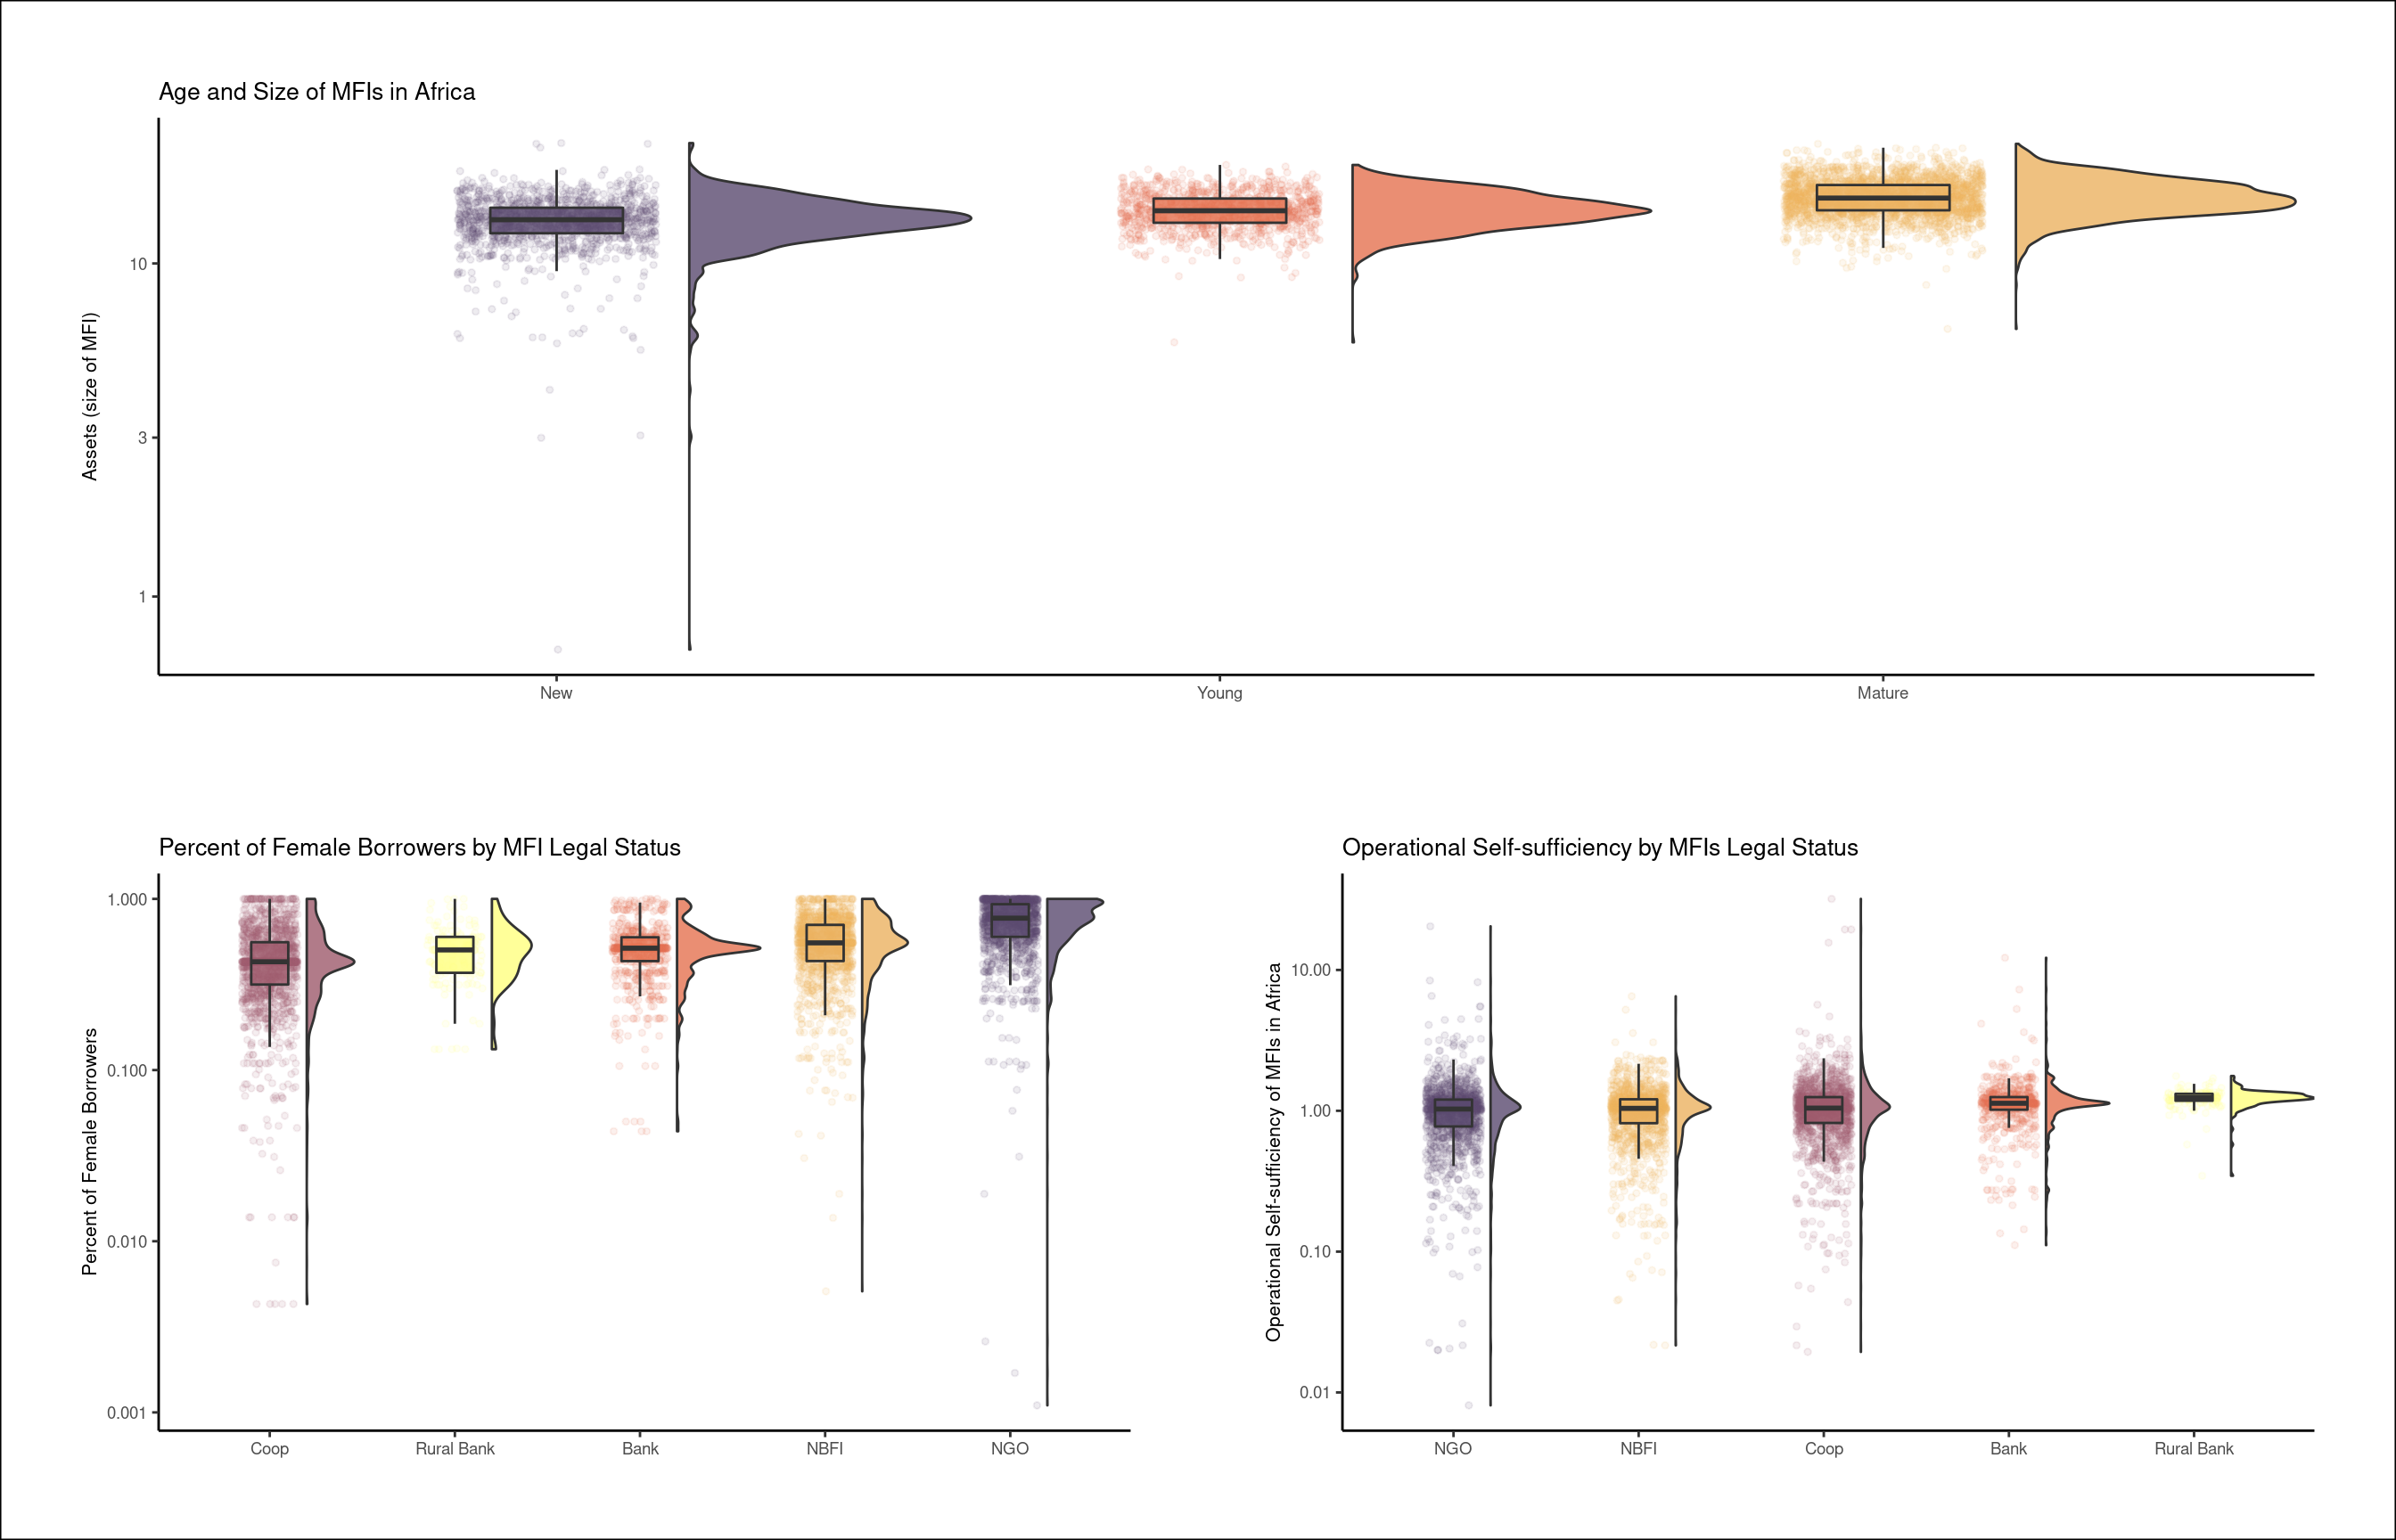
\includegraphics[width=8.8in]{_main_files/figure-latex/unnamed-chunk-165-1} 

}

\caption{Size and Age of Microfinance Institutions in Africa}\label{fig:unnamed-chunk-165}
\end{figure}

\end{landscape}

\newpage

\hypertarget{Introduction}{%
\chapter{Sources of Finance for Microfinance Institutions in Africa}\label{Introduction}}

\minitoc 
\chaptermark{Financing MFIs in Africa}

\newpage

\begin{center}

\textbf{ABSTRACT}

\end{center}

\begin{quote}
We examine the sources of finance for MFIs in Africa and their associated drivers. The sources of finance are leverage (debt-equity ratio), equity (capital to assets ratio), deposits (deposits to assets ratio), and donations (donations to assets ratio). Our analysis shows that at the firm level, size, age, legal status, and profitability drive financing alternatives, in line with theory. For example, asset structure varies inversely with leverage. At the country-level, institutional quality (KKM) varies inversely with deposits and donations. Intersstingly, coefficients of financial development are not statistically significant across all financial structure proxies, going against stylised facts on the macro-level drivers of firms' financing structure. Furthermore, we find that firm-level factors are more relevant in determining the financing structure of MFIs that country-level structures.
\end{quote}

\vspace{10mm}

\textbf{Key Words}: Finance, Capital, leverage, Donations, Debt, Deposits, Microfinance, Africa.

\vspace{5mm}

\textbf{JEL Classification}: G210, G230

\newpage

\newpage

\hypertarget{background-3}{%
\section{Background}\label{background-3}}

\textcite{bayai2016financing} cite institutional theory in explaining the way microfinance institutions (MFIs) in Africa fund their operations. They note that most MFIs tend to operate as Non-Governmental Organisations (NGOs) at the early stages. These NGOs derive substantial funding from donations and concessionary funds, given that commercial funders deem the MFIs too risky \autocite{ledgerwood1998microfinance,ledgerwood2006transforming}. Later, in the consolidation stage, the NGOs supplement their funds using government subsidies and equity funding. As they mature, they resort to deposits and debt whilst often using foreign donors as guarantees. At this stage, MFIs are likely to mutate from NGOs that focus on the social aspect of availing financial services to the financially excluded to the commercial model, where financial sustainability matters as much as social performance.

The transformation of MFIs from NGOs to the commercial model has raised concern over mission drift. Mission drift happens when MFIs focus more on profitability and less on the social aspect of reaching the unbanked \autocite{mia2017mission,ramus2017stakeholders}. Also, some researchers argue that the hybrid business model of most MFIs makes it challenging to integrate them into the formal financial system as financiers deem them too risky for the level of return they offer \autocite{campion1999institutional}. Conversely, the core argument for the institutional transformation of MFIs from the NGO, not-for-profit model, to the commercial model is access to capital markets. Advocates of the financial sustainability model of MFIs posit that capital market funding allows for improved corporate governance and reduces dependence on volatile donor funding \autocite{garmaise2013cheap,armendariz2013subsidy}. Financial sustainability also enables MFIs to reach more unbanked people in the long run \autocite{tchakoute2010there}.

Indeed, many MFIs are transitioning from the NGO not-for-profit model to the financial sustainability approach globally and in Africa. They strive to generate profit over and above meeting their social goal \autocite{hudon2010management,wagenaar2012institutional,kodongo2013individual}. Having grown on a donations dependent model, the shift to the commercial model has implied a change in the business model, and most importantly, a search for a steady source of capital beyond donations and subsidies \autocite{armendariz2013subsidy}.

Table 1 shows the sources of financing for MFIs in Africa. As expected, NGOs are least reliant on debt compared to other MFI models. Rural banks, commercial banks, Credit unions and NBFIs, respectively, have the most debt relative to assets. The picture is the exact opposite for capital to assets ratio, where NGOs lead while rural banks trail. NGOs have the lowest median deposits to assets ratio, probably arising from the legal restrictions on deposit mobilisation. Lastly, and not surprisingly, NGOs have the highest median donations to assets. While the data shows some regularity in terms of the legal status of MFIs, it is notable that some MFIs are shifting from the NGO model to the commercial model, mainly as commercial banks and NBFIs \autocite{sarma2011ngo,jia2016commercialization}. For the NGOs converting to the commercial model, the likelihood of alternative, sustainable sources of finance is a vital consideration.

This article examines the factors that determine the source of financing for MFIs in Africa, beyond the institutional life cycle proposition of \textcite{bayai2016financing}. Specifically, we explore the drivers of two primary capital structure indicators; leverage (debt to equity ratio), equity (capital to assets ratio), deposits (deposits to assets ratio) and finally, donations (donations to assets ratio). The existing literature on capital structure choices predominantly focuses on commercial (profit-oriented) firms \autocite{gropp2010determinants,liu2017optimal,matias2017there}. The drivers of financing for MFIs may differ from those of purely commercial firms because the social goals of MFIs may conflict with those of the commercial providers of funds. Nonetheless, the extant literature on the funding structure of MFIs mainly examines the link between capital structure and the performance and sustainability of MFIs \autocite{kyereboah2007determinants,khachatryan2017performance}.

In this respect, three studies by \autocite{kyereboah2007determinants,tchuigoua2014institutional,tchuigoua2015capital} closely resonate with our work. However, in these studies, the researchers focus chiefly on the determinants of leverage (debt-to-equity ratio) for MFIs and find leverage to be positively related to asset tangibility, size, past-due loans, and inversely related to creditor rights and risk; confirming the literature on capital structure. Profitability and credit ratings have a limited impact on capital structure, while financial development and legal tradition are significant. @\textcite{tchuigoua2014institutional} further finds that donations are negatively related to past-due loans and asset tangibility, implying donors do care about firm riskiness. None of the studies delves into the capital to assets ratio.

The contribution of our study goes beyond previous research in this area of scholarship in two respects: context and scope. Prior studies dwell exclusively on leverage (debt-equity ratio) while our study examines leverage, capital-assets ratio. The additional financing structure measures are essential for MFIs transitioning to the financial sustainability model as they must source funds externally. Besides, this study goes beyond that of \textcite{kyereboah2007determinants} that examined MFIs in Ghana only by focusing on Africa, thus allowing for cross-country comparisons. As \textcite{d2017ngos} cautions, research-based on geographically dispersed regions could mask important regional characteristics, as is the case with the research by \textcite{tchuigoua2014institutional} and \textcite{tchuigoua2015capital} Tchakoute-Tchuigoua that draws from a global dataset. This study will allow for deeper insights and comparison using data from a relatively homogeneous region by focusing on Africa. Such knowledge would, in turn, permit us to evolve more effective funding strategies to support and enable the unique added benefit of MFIs (that is, financial inclusion for the poor) that is particularly significant for emerging and developing economies and, in particular, Africa.

The following section highlights the study results, followed by a review of supporting theory and empirical literature. We then describe data and data sources, followed by the research method. We discuss the results and then conclude.

\hypertarget{summary-of-results-4}{%
\section{Summary of Results}\label{summary-of-results-4}}

The results of the data analysis show that the age of an MFI and governance/ institutional quality are the chief drivers of leverage (debt to equity ratio). The capital to assets ratio for MFIs in Africa has statistically significant relationships with MFI legal status, age, and legal tradition. MFI legal status, age, legal tradition, and profit margin are the key drivers of the deposits to assets ratio. MFI legal form, age, legal tradition, institutional quality, asset structure, private credit, and profit margin drive the donations to assets ratio. Young and mature MFIs have lower leverage relative to new MFIs. At the same time, institutional quality has a negative relationship with the debt to equity ratio. However, after removing influential observations, MFI legal form, asset structure, and profit margin become statistically significant leverage drivers. Specifically, NGOs have lower leverage than the commercial MFIs: banks, credit unions, NBFIs, and rural banks. Asset structure has a negative relationship with the debt to equity ratio, meaning that MFIs with more tangible assets finance their operations using relatively more equity than debt. Likewise, the profit margin negatively affects the debt to equity ratio, given that profits are part of equity.

NGOs have a consistently lower capital to assets ratio than other legal forms. Older MFIs have lower capital to assets proportions , while institutional quality negatively affects capital assets ratio. The relationship between the percentage of capital to assets and asset structure is mixed. Stock market capitalisation to GDP has a negative relationship with capital to assets ratio, while profit margin has a weak positive relationship. After removing outliers, assets structure shows a positive relationship with capital assets ratio, while private credit to GDP has a significant positive relationship with capital to assets ratio. NGOs have consistently lower deposits to assets ratio than other legal forms of MFIs.

In comparison, MFIs in civil and other legal traditions have a higher ratio than MFIs in civil law countries. Ceteris paribus, asset structure has a positive relationship with deposits to assets ratio. Without outliers, institutional quality private credit to GDP, stock market capitalisation to GDP, and profit margin also have a statistically significant relationship with deposits to assets ratio. Finally, the considerable drivers of the donations to assets ratio are MFI legal form, age, legal tradition, institutional quality, asset structure, private credit to GDP and profit margin. Specifically, NGOs have a higher ratio of donations to assets, while older MFIs and MFIs located in countries with civil law and other legal traditions have a lower ratio. Profit margin has a negative relationship with the donations to assets ratio, while institutional quality, assets structure, and private credit to GDP have the opposite effect.

\begin{landscape}

\begin{table}

\caption{\label{tab:unnamed-chunk-179}Summary Statistics for Categrical Independent Variables}
\centering
\fontsize{8}{10}\selectfont
\begin{tabu} to \linewidth {>{\raggedright}X>{\raggedright}X>{\raggedleft}X>{\raggedleft}X>{\raggedleft}X>{\raggedleft}X>{\raggedleft}X>{\raggedleft}X>{\raggedleft}X}
\toprule
Variable & Legal\_form & Mean & SD & Min & Q1 & Median & Q3 & Max\\
\midrule
Debt/Equity & NGO & 4.050 & 37.029 & -354.280 & 0.510 & 1.440 & 3.120 & 558.620\\
Debt/Equity & Bank & 4.109 & 4.308 & -15.490 & 2.130 & 3.590 & 5.625 & 74.810\\
Debt/Equity & NBFI & 3.480 & 30.336 & -440.870 & 0.720 & 1.975 & 4.290 & 531.260\\
Debt/Equity & Coop & 1.447 & 97.069 & -3567.280 & 1.250 & 3.090 & 5.405 & 585.240\\
Debt/Equity & Rural Bank & 6.717 & 3.205 & -8.530 & 5.255 & 6.200 & 7.617 & 20.430\\
\addlinespace
Capital/Assets & NGO & 0.418 & 0.752 & -18.353 & 0.221 & 0.381 & 0.637 & 12.150\\
Capital/Assets & Bank & 0.304 & 0.229 & -0.569 & 0.154 & 0.239 & 0.382 & 1.699\\
Capital/Assets & NBFI & 0.387 & 0.474 & -1.779 & 0.178 & 0.324 & 0.557 & 9.047\\
Capital/Assets & Coop & 0.196 & 0.665 & -14.819 & 0.109 & 0.208 & 0.351 & 11.269\\
Capital/Assets & Rural Bank & 0.176 & 0.243 & -0.133 & 0.103 & 0.137 & 0.162 & 1.982\\
\addlinespace
Donations/Assets & NGO & 0.225 & 0.234 & 0.000 & 0.000 & 0.160 & 0.344 & 1.274\\
Donations/Assets & Bank & 0.604 & 0.423 & 0.000 & 0.413 & 0.619 & 0.742 & 4.867\\
Donations/Assets & NBFI & 0.370 & 0.852 & 0.000 & 0.146 & 0.289 & 0.475 & 20.987\\
Donations/Assets & Coop & 0.601 & 0.356 & 0.000 & 0.443 & 0.582 & 0.724 & 5.702\\
Donations/Assets & Rural Bank & 0.844 & 0.993 & 0.298 & 0.684 & 0.747 & 0.791 & 8.960\\
\addlinespace
Donations/Assets & NGO & 0.095 & 0.227 & -0.003 & 0.000 & 0.011 & 0.082 & 2.598\\
Donations/Assets & Bank & 0.014 & 0.075 & 0.000 & 0.000 & 0.000 & 0.000 & 1.304\\
Donations/Assets & NBFI & 0.037 & 0.124 & -0.001 & 0.000 & 0.000 & 0.013 & 1.706\\
Donations/Assets & Coop & 0.020 & 0.079 & 0.000 & 0.000 & 0.001 & 0.011 & 1.617\\
Donations/Assets & Rural Bank & 0.001 & 0.010 & 0.000 & 0.000 & 0.000 & 0.000 & 0.077\\
\bottomrule
\multicolumn{9}{l}{\rule{0pt}{1em}\textit{Source: }}\\
\multicolumn{9}{l}{\rule{0pt}{1em}Authors' construction from the MIX data}\\
\multicolumn{9}{l}{\rule{0pt}{1em}\textit{Note: }}\\
\multicolumn{9}{l}{\rule{0pt}{1em}\textsuperscript{1} N = 4782}\\
\multicolumn{9}{l}{\rule{0pt}{1em}\textsuperscript{2} Legal status include NGO, Non-Bank Financial Institutions (NBFIs), Credit Unions, and Banks}\\
\multicolumn{9}{l}{\rule{0pt}{1em}\textsuperscript{3} Age has mature MFIs older than 8 years, young ones (4 - 8 years), and new ones that are 4 years or less}\\
\end{tabu}
\end{table}

\end{landscape}

\hypertarget{theoretical-framework}{%
\section{Theoretical Framework}\label{theoretical-framework}}

Like commercial firms, MFIs draw their capital from equity, debt (including deposits). Unlike commercial firms, MFIs have a substantial source of capital in the form of donations and subsidies (D'Espallier et al., 2013). As noted, despite the notable difference in financing structure, the empirical research on the financing of MFIs mainly relates to debt-equity mix \autocite{kyereboah2007determinants,tchuigoua2014institutional,tchuigoua2015capital}. This study seeks to examine the drivers of the more comprehensive financing structure of MFIs concerning leverage and capital (equity) to assets ratio. The study draws its theoretical frame from two theories: the capital structure and institutional (life cycle) theories.

The capital structure theories seek to explain the mix of long-term debt and equity in the financing structure of enterprises \autocite{ehrhardt2016corporate}. The dominant literature in this respect revolves around the Modigliani \& Miller capital structure theories, of which the trade-off theory against predominant \autocite{sun2016ownership}. The classic trade-off theory holds that the debt-equity mix is relevant insofar as it generates a debt tax shield that organisations balance with the costs of possible financial distress that comes with high debt levels \autocite{liu2017optimal}. Further, financial distress explains why firms favour easily negotiable debt, making firms approve bank loans in place of sourcing debt funds via capital markets \autocite{de2011firms}.

The implication is that mature, profitable firms rely on internal capital sources as do firms with little cash flows and intangible assets. In this case, the trade-off theory corresponds with the pecking order theory of Donaldson and Fox (1961) and \textcite{myers1984corporate}, which posits that firms issue capital in a predetermined order, usually starting with the cheapest internal sources of funds while maintaining a reserve borrowing capacity. In the case of MFIs, we presume that donations and subsidies would come first in the pecking order. The reserve borrowing capacity allows firms to arrange debt funds quickly in case of profitable opportunities that arise. Moreover, the trade-off theory corresponds with the proposition by \textcite{bayai2016financing} that the capital structure of MFIs evolves with the institutional life-cycle of firms. Younger firms are more proportionately reliant on donations and concessionary funds. Older firms more inclined to commercial funding.

\textcite{bradley1984existence} extended the trade-off theory, showing that, under certain conditions, the tax disadvantage of debt at the individual level offset the tax disadvantage at the corporate level. The result was the introduction of leverage related costs to the classical trade-off theory. These costs include the bankruptcy costs, agency costs of debt, the loss of non-debt tax shields (such as accelerated depreciation and investment tax credits). The additional leverage related costs mean that firms seek to balance the tax benefits of debt and the leverage-related costs. \textcite{miao2005optimal} show that the choice of financing mix relates to these non-debt tax shields, in addition to financial and trade cycles. Hence the capital structure is firm-specific and mean-reverting. Still, the capital structure theories cannot explain the observed under-leveraged firms. Moreover, while the profit motive drives commercial firms, the capital structure theories may not fully apply to hybrid firms with a dual mission, like MFIs.

The institutional theory does have some congruence with the capital (financial) structure of MFIs. The observed rise in debt financing and the concurrent drop in donations could point to a shift by MFIs towards a financially sustainable MFI model. The pressure to move towards the financial sustainability model could reflect a broader change in the MF industry or result from pressure from donors, signalling fatigue and the intent to withdraw or reduce funding. The pressure would be incredibly intense for MFIs that are highly dependent on donations \autocite{powell2012new}, underlining the role of donors such as USAID in the push towards sustainability \autocite{bateman2010doesn}. Although the institutional theory cannot fully account for the MFIs that have not changed from NGOs to commercial models, the changing capital structures indicate that financial sustainability is gaining traction. Figure 6.4 shows that even without a change in legal forms, the proportion of donations to MFIs in Africa is dropping. The following section details the empirical approach adopted in the study.

\hypertarget{method-2}{%
\section{Method}\label{method-2}}

The study adopts the fixed and random effects models depending on the outcome of the Hausman tests (see appendix 2). Following \textcite{roberts2013endogeneity}. We consider the model that follows.

\(Y_{it} = \beta_{0} + \beta_{1}X_{it} + \mu_{it}\)

Further, assume that,

\(\mu_{it} = C_{i} + \epsilon_{it}\)

Where \(c_{i}\) captures the aggregate effects of the unobserved, time-invariant explanatory variables for \(Y_{it}\) . Further, assume that \(e_{it}\) has zero mean conditional on \(X_{it}\). In the case where \(C_{i}\) and \(X_{it}\) are correlated, then \(C_{t}\) is a fixed effect; otherwise, it is a random effect. Note that the existence of fixed effects implies the presence of endogeneity. For random effects, on the other hand, endogeneity is not a concern. However, the random-effects model affects the computation of standard errors (Roberts \& Whited, 2013).

Thus, the fixed effects models seek the causes of changes within an entity. The fixed-effects model does this by controlling for all time-invariant differences between the individuals, so the estimated coefficients of the fixed-effects models cannot be biased because of omitted time-invariant characteristics, such as culture \autocite{torres2007panel}. To deal with the endogeneity inherent in the fixed effects model, researchers recommend two strategies. The first approach involves the inclusion of firm-specific intercepts by running the least squares dummy variable regression. The method is not feasible with medium to large datasets. In the alternative within-estimator approach, researchers apply OLS to the deviations-from-the-within estimator, eliminating the fixed effect prone to endogeneity. The within-estimator regression is as follows \footnote{For a more detailed but simplified discussion on the derivation and application of the within-estimator, refer to Roberts and Whited (2013), pp.~558.}.

\begin{equation}
Y_{it} = \beta_{1} \Delta X_{it} + \Delta \mu_{it}
\end{equation}

However, the model does not deal with the potential endogeneity between \(\Delta X_{it}\) and \(\mu_{it}\). Differencing also reduces the efficiency of estimates if the fixed effect (differenced out of the model) and the dependent variable correlate strongly \autocite{clark2015should}. Consequently, we run both fixed and random effects, even where the Hausmann test recommends one over the other.

\hypertarget{variables-definitions-and-data-sources}{%
\subsection{Variables Definitions and Data Sources}\label{variables-definitions-and-data-sources}}

We source panel data from the Microfinance Information Exchange (MIX) pooled database, the Worldwide Governance Indicators (WGI), and World Development Indicators (WDI) from the World Bank databases. Table 6.2 below describes the variables.

\begingroup\fontsize{9}{11}\selectfont

\begin{longtabu} to \linewidth {>{\raggedright}X}
\caption{\label{tab:unnamed-chunk-180}Description of Variables}\\
\toprule
Variable\_Description\\
\midrule
\endfirsthead
\caption[]{\label{tab:unnamed-chunk-180}Description of Variables \textit{(continued)}}\\
\toprule
Variable\_Description\\
\midrule
\endhead

\endfoot
\bottomrule
\multicolumn{1}{l}{\rule{0pt}{1em}Source: Authors' construction from the literature}\\
\multicolumn{1}{l}{\rule{0pt}{1em}\textit{Notes}}\\
\multicolumn{1}{l}{\rule{0pt}{1em}\textsuperscript{1} MIX Database on www.themix.org and https://datacatalog.worldbank.org/dataset/mix-market}\\
\multicolumn{1}{l}{\rule{0pt}{1em}\textsuperscript{2} WDI on https://databank.worldbank.org/source/world-development-indicators.}\\
\multicolumn{1}{l}{\rule{0pt}{1em}\textsuperscript{3} WGI/ KKM on https://databank.worldbank.org/source/worldwide-governance-indicators.}\\
\multicolumn{1}{l}{\rule{0pt}{1em}\textsuperscript{4} GFDD on https://www.worldbank.org/en/publication/gfdr/data/global-financial-development-database}\\
\endlastfoot
1. Debt-to-Equity Ratio: The ratio of total liabilities to equity, the amount of leverage supported by each unit of capital contributed by shareholders. The ratio shows how an MFI finances its portfolio of assets beyond equity capital to cushion or absorb losses when total assets fall short of all liabilities. Much of the extant research examines the debt-equity mix and its relationship with the performance of MFIs\\
2. Deposits to Total Assets: The ratio of deposits to assets that aids in determining the extent to which MFIs use deposits to finance assets. NGOs transitioning to the commercial model can mobilise deposits  to fund their operations over and above donations and equity\\
3. Capital to Assets Ratio: The ratio of total equity to total assets and a slightly modified reciprocal debt-to-equity ratio. Hence, it captures the ability to meet obligations and to absorb unexpected losses using capital contributions by the owner (Kimmel, Weygandt, \& Kieso, 2018)\\
4. Current Legal Status: The legal forms of registration of an MFI are as follows; Commercial Bank, Non-Bank Financial Institution (NBFI), Non-Governmental Organization (NGO), Credit Union/ Cooperative, or Rural Bank. The legal status may dictate the profit orientation and sources of capital for the MFIs. The legal status of an MFI may impact the financing structure in several ways. First, legal status or form typically restricts NGOs from taking deposits, which lowers the debt-equity ratio and deposits to assets, raising the capital asset ratio. Also, NGOs may not venture into capital markets for funds, given their mostly not-for-profit orientation. The opposite is the case for MFIs of commercial banks legal form whose legal status allows for deposits.\\
\\
\addlinespace
5.  Age: MIX classifies MFIs into three categories depending on the time that has elapsed since the MFI started operations- new (0-4 years), young (4-8 years) and mature (over eight years). The variable is hence a dummy. Older firms are likely better established, have a solid reputation and hence likely to attract more debt and deposits. The institutional life cycle view of Bayai and Ikhide (2016) captures the correspondence between age and debt.\\
\\
6. Legal Tradition (Legal): The indicator is a dummy variable with common law countries coded 0, civil law countries 1, and 2 otherwise as per the classification by Oto-Peralías and Romero-Ávila (2014). Typically, common law countries have relatively better financial infrastructure that allows firms to access financial markets easily. Hence, MFIs in common law countries may exhibit higher debt and equity ratios in their capital structures than those in common law and other legal traditions. (Schnyder, Gerhard, Mathias Siems, \& Ruth V. Aguilera, 2018)\\
\\
7. Size (Log of Total Assets): We proxy the size of MFI with the natural logarithm of total assets, again using MIX data. Assets are supported by the sum of capital and liabilities or, equivalently, the total value of resources owned or controlled by the MFI resulting from past and current activities and from which the MFI derives future benefits. We expect firms with more assets to have a higher debt capacity and more debt-to-equity ratios, and lower capital to equity ratios. Large firms draw their strength from holding diversified investments and hence higher capacity to absorb risk. Besides, they have easy access to debt markets(Kurshev \& Strebulaev, 2015). Furthermore, these firms are likely to attract more deposits, given the trust they inspire in depositors and their marketing reach (Kimmel et al., 2018). We hypothesise that donations vary positively with the size of MFI, as large, older firms have established a reputation with donors.\\
\addlinespace
\\
7. Governance/ Institutional Quality (KKM): We create the country level KKM index using the first principal component of the WGI available in the World Bank databases. The index captures the institutional quality in corruption control, government effectiveness, political stability, the rule of law, and voice and accountability (Kaufmann, Kraay, \& Mastruzzi, 2011). Firms in countries with better governance can quickly raise debt finance due to ease of contract enforcement — the result, a high debt-equity ratio and a low capital asset ratio. Similarly, the level of deposits mobilisation may be higher in better-governed countries arising from consumer confidence in legislation relating to deposits protection (La Porta, Lopez-de-Silanes, \& Shleifer, 2013; Allen et al., 2014). Lastly, MFIs in countries with low KKM may have higher donations as donors opt to circumvent corrupt government channels. We use the terms institutional quality and governance interchangeably throughout the text\\
\\
8. Private Credit to GDP: We capture the total amount of credit advanced to the private sector by financial intermediaries as a proxy for capital markets development concerning the banking sector following Ito and Kawai (2018). The data source is the Global Financial Development Database, GFDD, of the World Bank (See note 4). Private credit to GDP represents the financial resources provided to the private sector by domestic money banks as a share of GDP. Domestic money banks comprise commercial banks and other financial institutions that accept transferable deposits, such as demand deposits. The data is available in WDI. Financial sector development is central to the acquisition of both equity and debt financing. We hypothesise a high debt to equity ratio, and deposits to assets ratios in countries with more robust financial sectors as financial institutions tend to be highly leveraged.\\
\\
\addlinespace
9. Stock market capitalisation to GDP: We capture the extent of stock market development using the ratio of stock market capitalisation to GDP to proxy how firms can raise equity capital. Although Africa's equity markets are thin, some relatively large stock markets like South Africa, Kenya, and Ghana exist. The data are from the GFDD.\\
\\
11. Education: Education is the ratio of gross secondary school enrolment to gross primary school enrolment that captures the extent of graduation from elementary to secondary education and the overall literacy rate. The data is available in the WDI. We hypothesise a positive relationship between education and debt/equity ratio, implying a lower capital asset ratio. Similarly, education may enhance the capacity of the populace to use financial products like savings, hence a higher deposit to assets ratio.  Also, education may directly or indirectly influence financial sector development, which eases the acquisition of capital in financial markets (Allen et al., 2014).\\
\\
12. Asset Structure (Tangibility): Asset structure is is measured as the ratio of non-current assets to total assets of an MFI (Microfinance Information Exchange (MIX), 2019). The ratio indicates the extent of investment in physical infrastructure, a significant issue in constraining banking for the poor due to the perceived lack of scale economies to warrant the erection, for instance, of brick and mortar branches (Ledgerwood, 1998). MFIs with a more significant physical presence are likely to attract more deposits. Therefore, they also have a higher capacity to borrow and service debt. Further, tangible assets serve as collateral to protect lenders from the moral hazard problem (Jensen \& Meckling, 1976), and hence a positive relationship between debt and asset tangibility (Titman \& Wessels, 1988; Kyereboah-Coleman, 2007a).\\
\addlinespace
\\
13. Profit Margin: The profit margin is the net operating income divided by financial revenue. The ratio represents the ability of MFIs to generate income from the core mandate of offering financial services like lending, savings, insurance, and so on. Profitability may enhance the capacity of an MFI to secure debt, thus leading to a higher debt to equity ratio and low capital to assets ratio. The opposite is the case when an MFI retains earnings and hence raises the level of equity.\\
\\*
\end{longtabu}
\endgroup{}

\hypertarget{exploratory-data-analysis-2}{%
\section{Exploratory Data Analysis}\label{exploratory-data-analysis-2}}

Figure 1 shows the correlation matrix and scatter plots for the numeric variables used in this work's empiricalmodel. Furthermore, the debt-to-equity ratio, capital-to-assets ratio, deposits to assets ratio, and donations to assets ratio (the first four entries of the rows and columns) are the dependent variables. The rest are the independent variables, including the donations to assets ratio. The main diagonal shows the distribution of the representative variables in place of correlations of a variable with themselves. The main diagonal shows that most variables are highly skewed, except for assets. The lower half of the Figure shows the pairwise scatter plots between the variables, with the axis interpreted as we do correlation matrices as described next.

\begin{landscape}

\begin{table}

\caption{\label{tab:unnamed-chunk-181}Summary Statistics}
\centering
\fontsize{10}{12}\selectfont
\begin{tabu} to \linewidth {>{\raggedright}X>{\raggedleft}X>{\raggedleft}X>{\raggedleft}X>{\raggedleft}X>{\raggedleft}X>{\raggedleft}X>{\raggedleft}X}
\toprule
Variable & Mean & SD & Min & Q1 & Median & Q3 & Max\\
\midrule
Debt\_to\_equity\_ratio & 3.201 & 58.609 & -3567.280 & 0.900 & 2.430 & 4.880 & 585.24\\
Capital\_asset\_ratio & 0.321 & 0.602 & -18.353 & 0.153 & 0.273 & 0.478 & 12.15\\
Deposits\_to\_total\_assets & 0.444 & 0.577 & 0.000 & 0.171 & 0.411 & 0.642 & 20.99\\
Donations\_assets\_ratio & 0.043 & 0.147 & -0.003 & 0.000 & 0.001 & 0.019 & 2.60\\
Assets & 14.946 & 2.262 & 0.693 & 13.540 & 14.858 & 16.416 & 22.98\\
\addlinespace
Kkm & 0.003 & 2.006 & -5.233 & -1.304 & -0.114 & 1.628 & 7.37\\
Education & 0.387 & 0.144 & 0.075 & 0.273 & 0.386 & 0.487 & 1.05\\
Pcrdbgdp & 2.719 & 0.685 & 0.298 & 2.386 & 2.758 & 3.052 & 6.88\\
Stmktcap & 1.141 & 1.473 & 0.000 & 0.000 & 0.000 & 2.428 & 5.80\\
Gdp\_growth\_annual & 5.310 & 3.590 & -46.082 & 4.000 & 5.420 & 6.723 & 33.63\\
\addlinespace
Profit\_margin & -7.739 & 513.299 & -35495.625 & -0.181 & 0.048 & 0.189 & 6.20\\
\bottomrule
\multicolumn{8}{l}{\rule{0pt}{1em}\textit{Source: }}\\
\multicolumn{8}{l}{\rule{0pt}{1em}Authors' construction from MIX data}\\
\end{tabu}
\end{table}
\end{landscape}

\begin{landscape}

\begin{figure}

{\centering 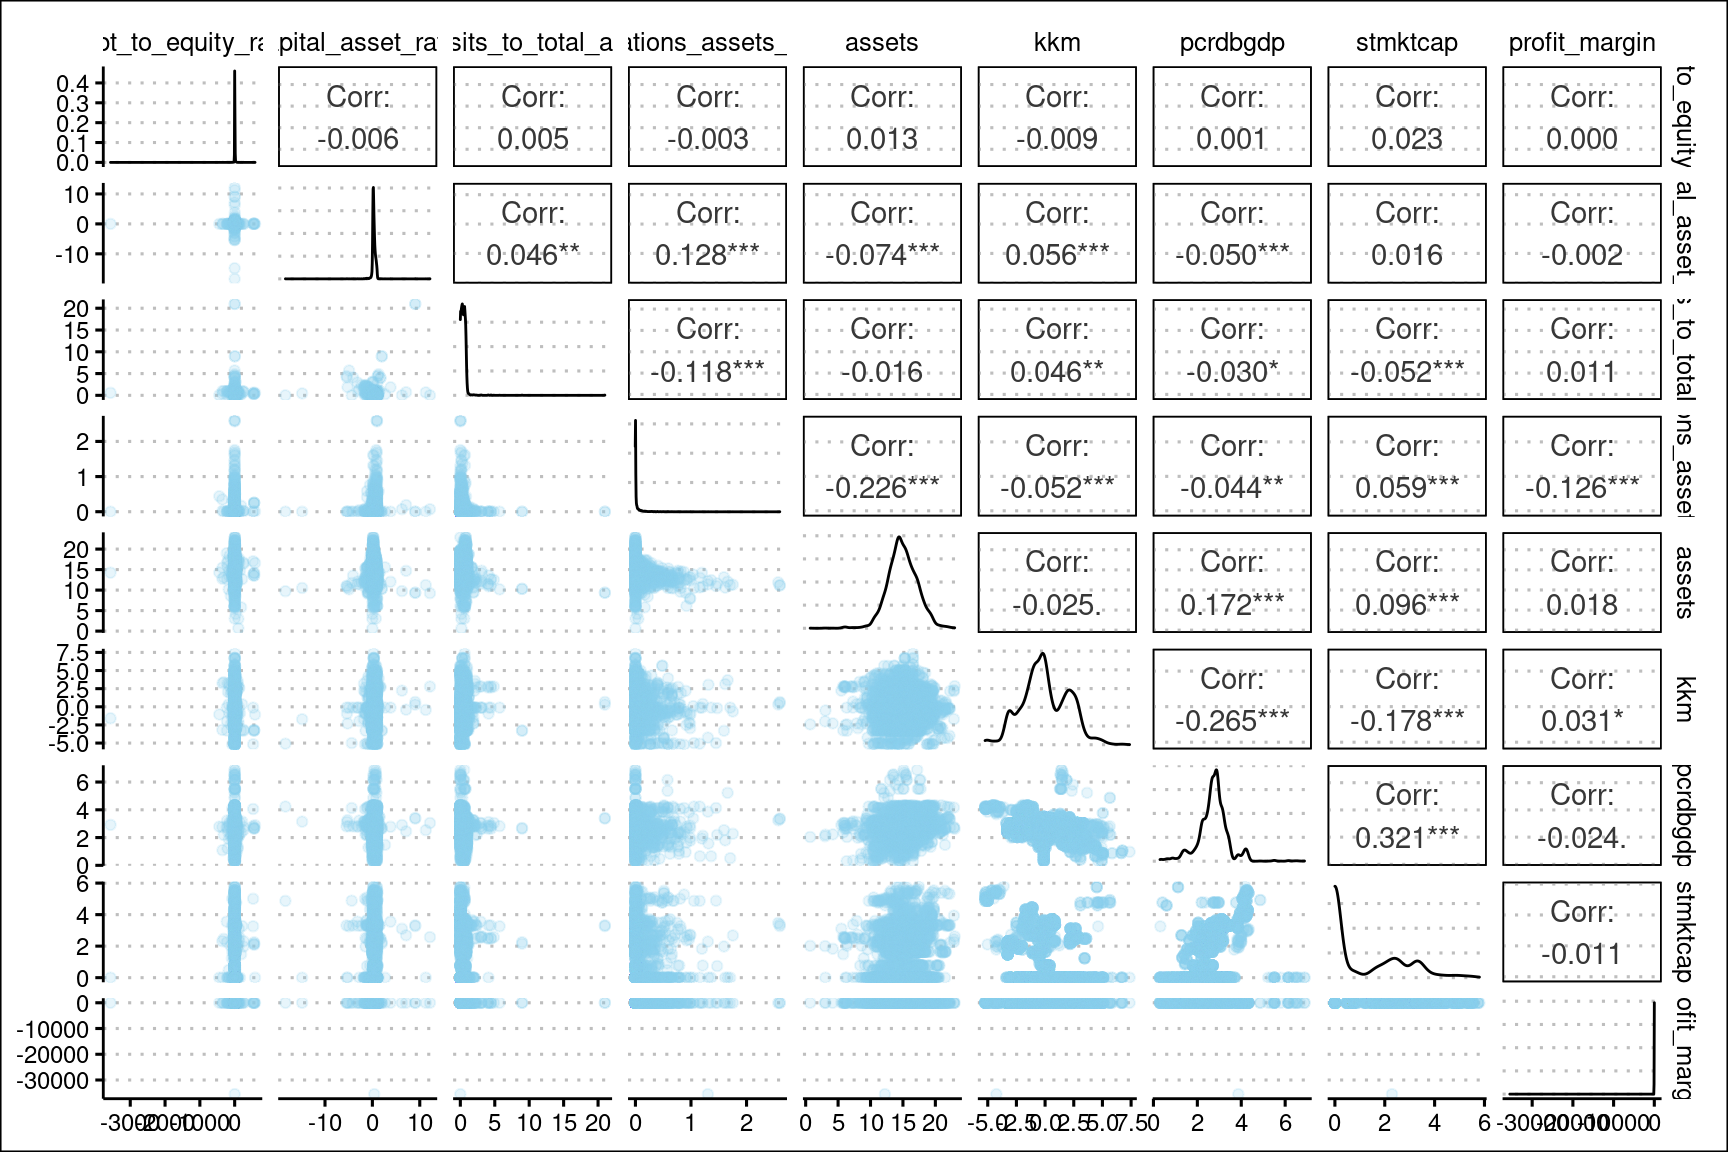
\includegraphics[width=8.8in]{_main_files/figure-latex/unnamed-chunk-182-1} 

}

\caption{Correlation Matrix for Independent Variables}\label{fig:unnamed-chunk-182}
\end{figure}

\end{landscape}

There is a substantial negative and significant relationship between capital-asset-ratio (which captures the ratio of equity capital to total assets) and deposits-assets-ratio for dependent variables. The correlations indicate that for MFIs that garner deposits, the injection of equity capital is not a priority as these MFIs, like commercial banks, tend to leverage on deposits and just put in enough equity to meet regulatory requirements. The debt to equity ratio and the deposits to asset ratio have a significant positive relationship, although the magnitude is not high. The capital to asset ratio and debt to equity ratio has no meaningful association. For the dependent variables, the highest observed correlation is between education on the one hand and the proxies for capital market development; private credit to GDP and stock market capitalisation to GDP, at 0.461 and 0,538, which is in line with the literature \autocite{allen2013resolving,allen2014african}. Consequently, we exclude education from our regressions.

Finally, except for the debt to equity ratio, the other three independent variables significantly correlate with the dependent variables. Specifically, the debt to equity ratio has a low but significant correlation with the other dependent and independent variables. The capital asset ratio has no statistically significant correlation with profit margin and stock market capitalisation to GDP. Likewise, donations have no significant correlation with GDP growth and education, while deposits exhibit a substantial correlation with donations, institutional quality/ governance, and stock market capitalisation to GDP. While correlation does not imply causation, these results point to the need for further investigation. The following section on regression models revisits this result for an in-depth interrogation of the relationships. Table 6.3 shows the summary statistics for the numeric variables while Table 6.4 summarises the categorical variables.

Figure 2 shows the breakdown of the dependent variables across MFI legal status. Note that rural banks and commercial banks have the highest median debt to equity and deposits to assets ratios, followed by credit unions, NBFI, and NGOs. The former could indicate ease in accessing capital markets. At the same time, deposits reflect the capacity of banks to mobilise deposits. Their focus on niche rural markets with the unbanked populace makes it easier to garner deposits for rural banks. The visualisation rightly shows that rural banks, commercial banks and cooperatives have the highest deposits to assets ratio.

Consequently, commercial banks, cooperatives, and rural banks have the lowest capital to assets ratio. The results show that commercial banks and rural banks emphasise offering a broader range of financial services, specifically savings products in place of credit alone. For NGOs, Garnering deposits is a challenge due to legal hurdles. Coupled with the emphasis on the social aspect of reaching the poor, NGOs would have a more significant difficulty accessing commercial funding compared to other legal types of MFIs. Reinforcing the welfare approach to microfinance, NGOs have the highest median donations to assets ratios, followed by NBFIs, while commercial banks and rural banks come last. These results arise out of the mission of MFIs, where donors fund MFIs that explicitly focus on social aspects of reaching the unbanked- meaning that donors still do value the welfare approach to microfinance.

Finally, Figure 6.4 shows the trends in the dependent variables over time, with the debt to equity ratio trending gradually upwards while the capital to assets ratio trends downwards. It shows that MFIs have steadily been increasing their debt capital over this period as they grow and get to access capital markets. Likewise, deposits have been trending upwards as more MFIs reach a higher number of consumers or as they mature and get the legal mandate to garner deposits. The trend for the donations to assets ratio is like literature in microfinance suggests; donors have gradually reduced their relative contribution to MFIs. Alternatively, MFIs are less reliant on donations as they grow, given that donations form a decreasing proportion of their assets base. The implication here is that both donors and MFIs have gradually embraced the financial sustainability approach to microfinance, thus requiring MFIs to be financially sustainable while fulfilling their social mandate. Next, we discuss the results of the regressions.

\begin{landscape}

\begin{figure}

{\centering 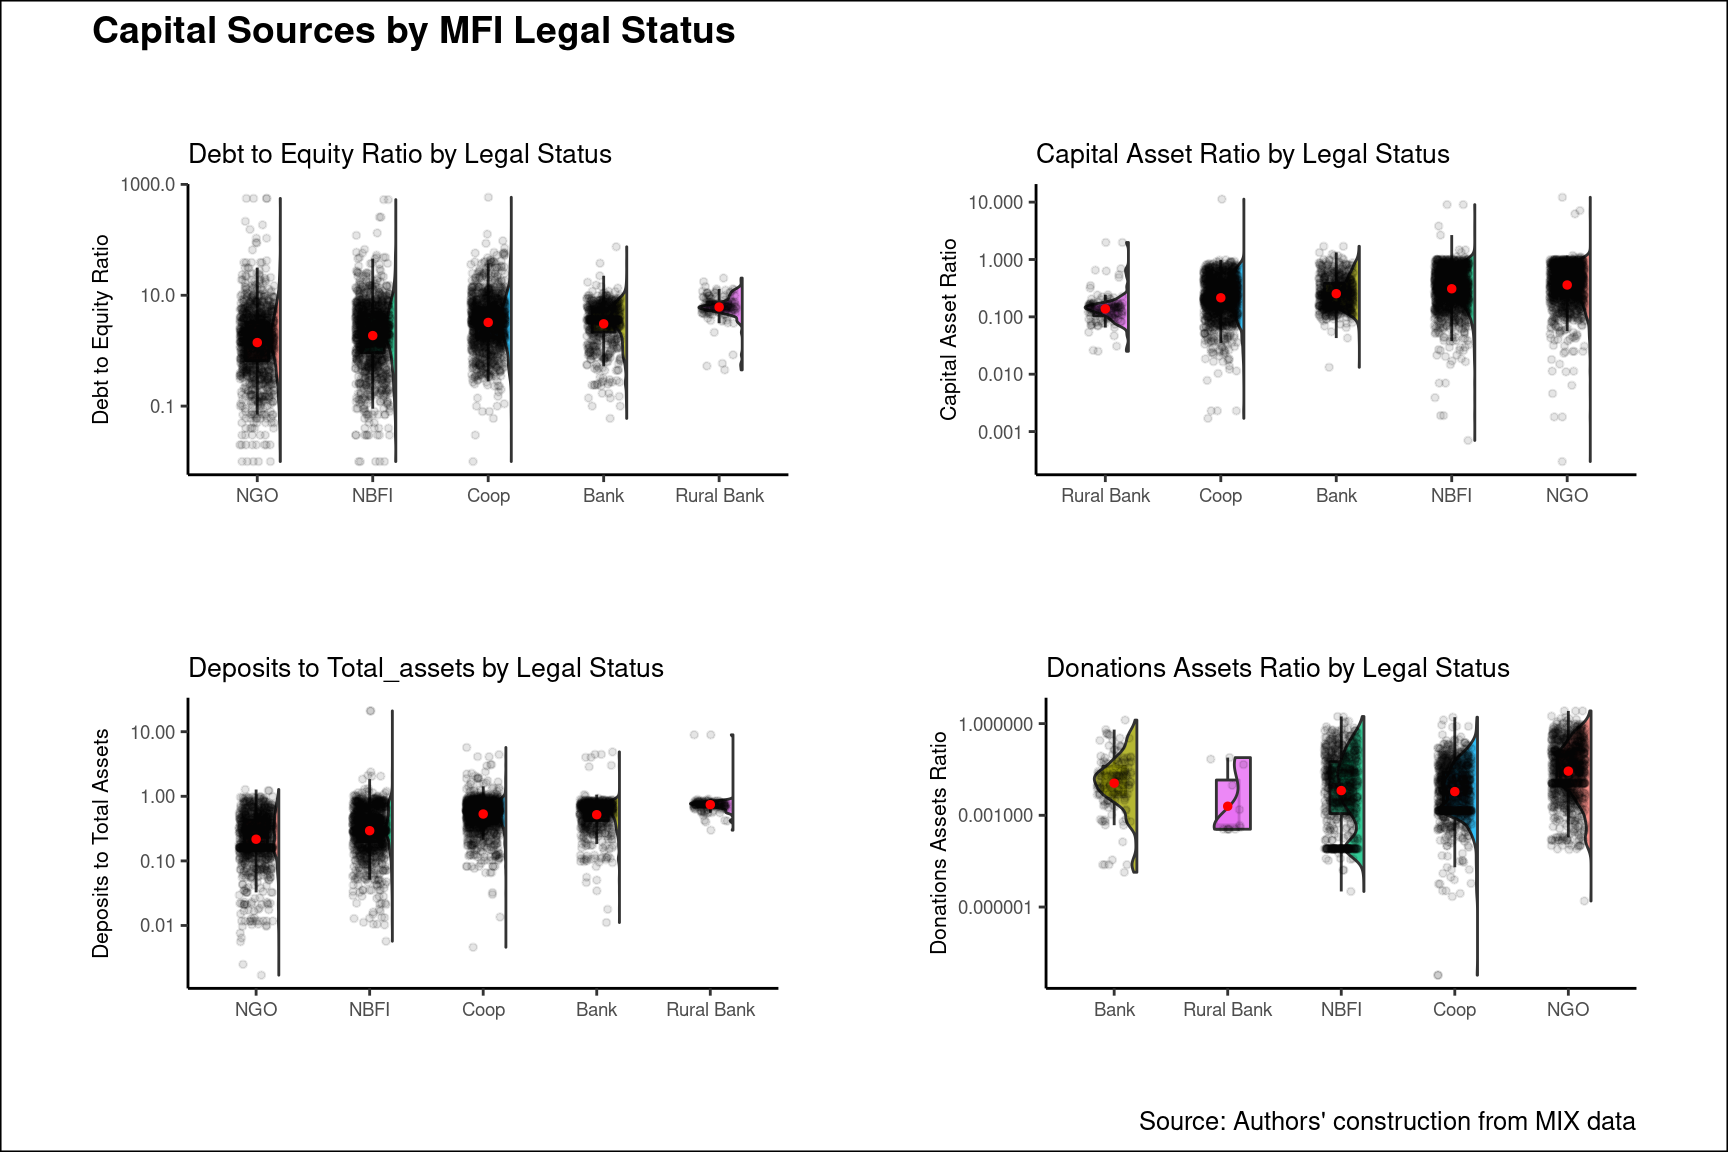
\includegraphics[width=8.8in]{_main_files/figure-latex/unnamed-chunk-183-1} 

}

\caption{Capital Sources by MFI Legal Status}\label{fig:unnamed-chunk-183}
\end{figure}

\end{landscape}

\begin{landscape}

\begin{figure}

{\centering 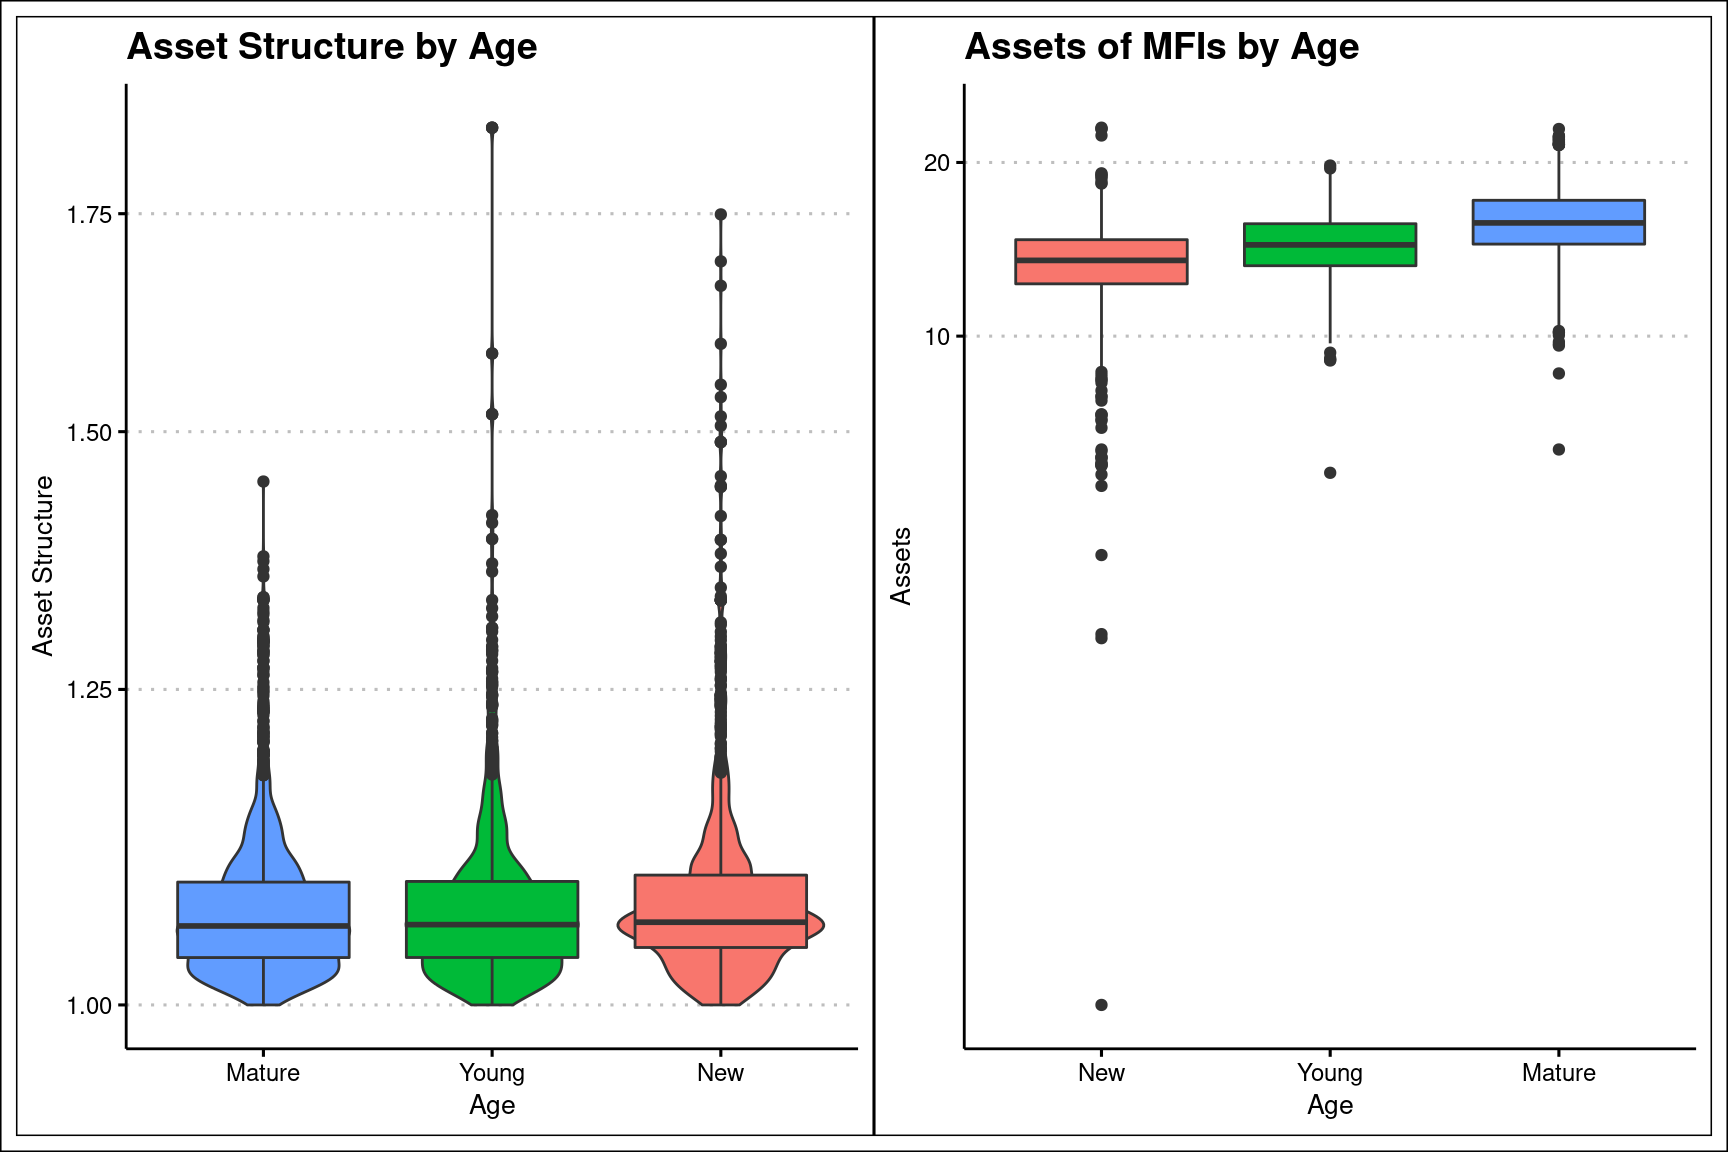
\includegraphics[width=8.8in]{_main_files/figure-latex/unnamed-chunk-184-1} 

}

\caption{Assets, Asset Structure, and Profit margin of MFIs in Africa}\label{fig:unnamed-chunk-184}
\end{figure}

\end{landscape}

\begin{landscape}

\begin{figure}

{\centering 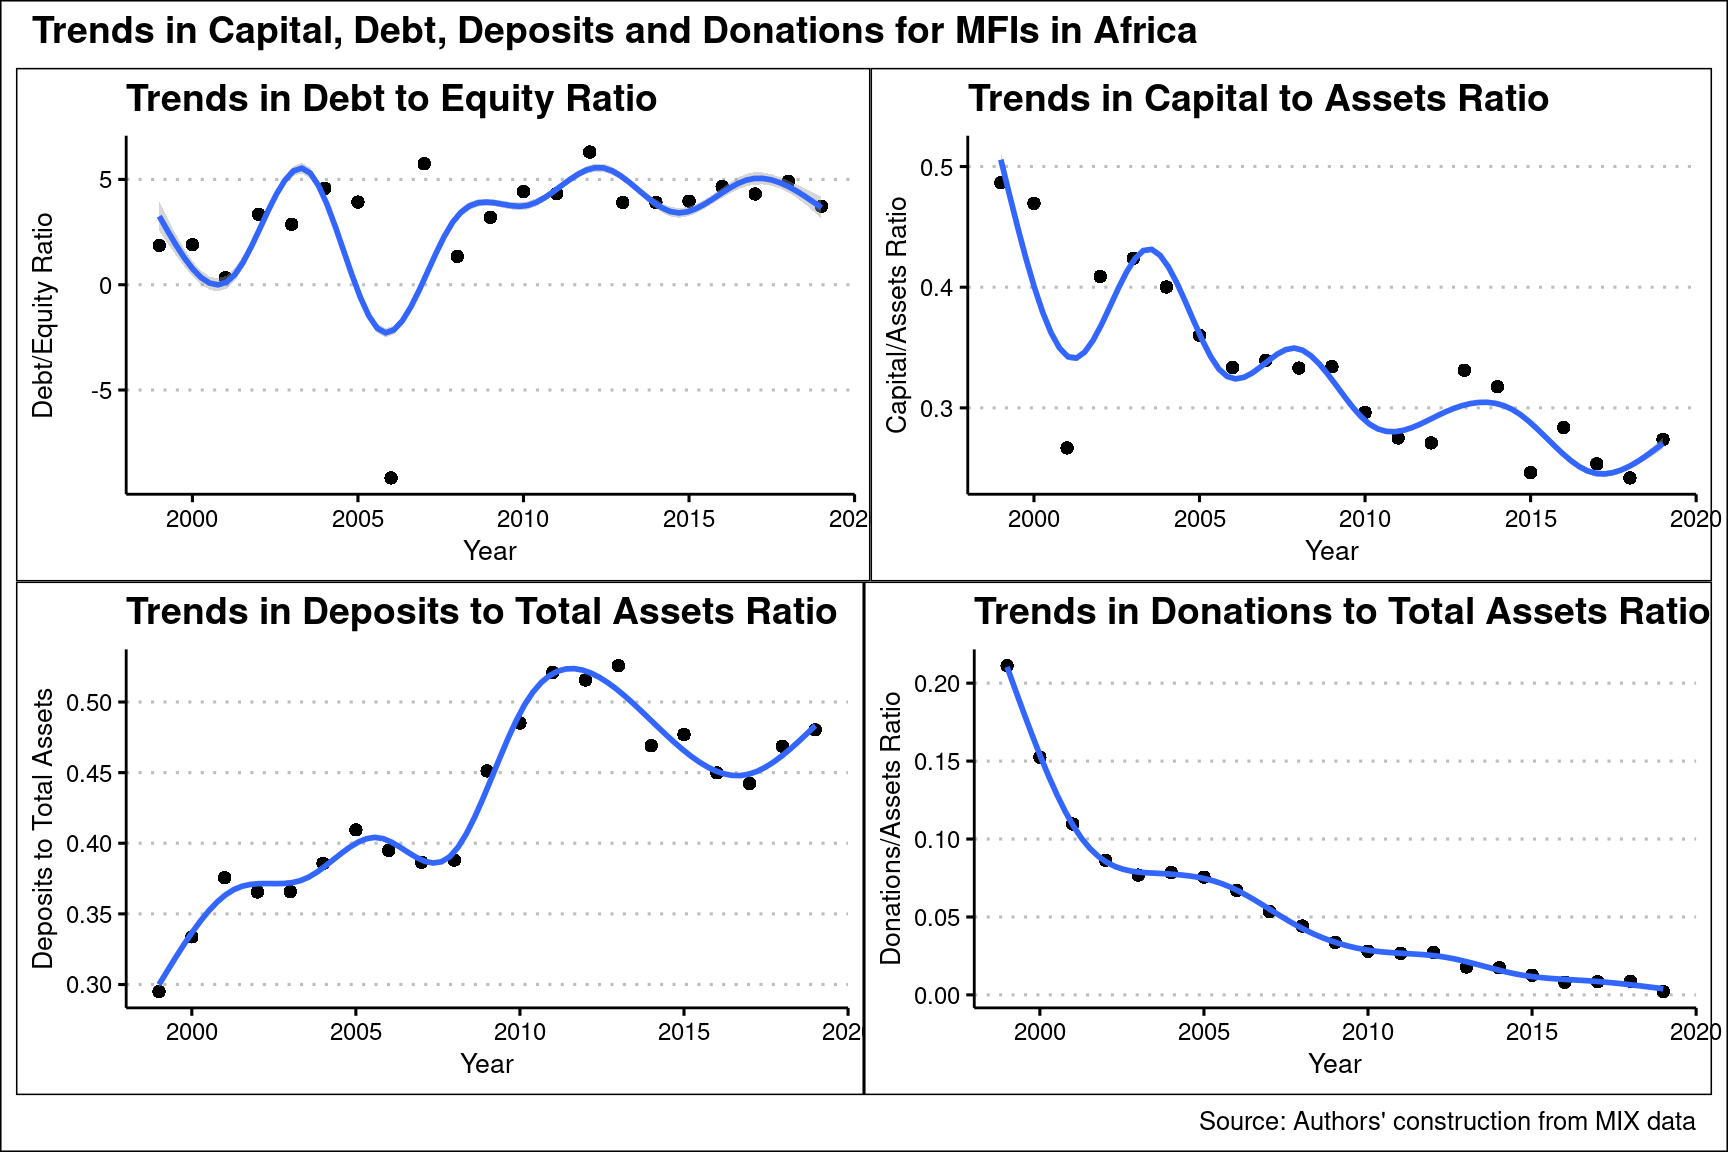
\includegraphics[width=8.8in]{_main_files/figure-latex/unnamed-chunk-185-1} 

}

\caption{Trends in Capital, Debt, Deposits, and Donations}\label{fig:unnamed-chunk-185}
\end{figure}

\end{landscape}

\begin{table}

\caption{\label{tab:unnamed-chunk-186}Summary Statistics for Categrical Independent Variables}
\centering
\fontsize{9}{11}\selectfont
\begin{tabu} to \linewidth {>{\raggedright}X>{\raggedleft}X>{\raggedleft}X>{\raggedleft}X>{\raggedleft}X>{\raggedleft}X>{\raggedleft}X>{\raggedleft}X>{\raggedleft}X}
\toprule
Variable & N & Mean & SD & Min & Q1 & Median & Q3 & Max\\
\midrule
asset\_structure & 4782 & 0.076 & 0.069 & 0.000 & 0.035 & 0.060 & 0.092 & 0.86\\
assets & 4782 & 14.946 & 2.262 & 0.693 & 13.540 & 14.858 & 16.416 & 22.98\\
pcrdbgdp & 4782 & 2.719 & 0.685 & 0.298 & 2.386 & 2.758 & 3.052 & 6.88\\
stmktcap & 4782 & 1.141 & 1.473 & 0.000 & 0.000 & 0.000 & 2.428 & 5.80\\
profit\_margin & 4782 & -7.739 & 513.299 & -35495.625 & -0.181 & 0.048 & 0.189 & 6.20\\
\bottomrule
\multicolumn{9}{l}{\rule{0pt}{1em}Source: Authors' construction from the MIX data}\\
\multicolumn{9}{l}{\rule{0pt}{1em}\textit{Note: }}\\
\multicolumn{9}{l}{\rule{0pt}{1em}\textsuperscript{1} Legal status include NGO, Non-Bank Financial Institutions (NBFIs), Credit Unions, and Banks}\\
\multicolumn{9}{l}{\rule{0pt}{1em}\textsuperscript{2} Age has mature MFIs older than 8 years, young ones (4 - 8 years), and new ones that are 4 years or less}\\
\end{tabu}
\end{table}

\hypertarget{regression-results}{%
\section{Regression Results}\label{regression-results}}

This section discusses the output from the regression models, starting with the debt to equity ratio, the capital to assets ratio, the deposits to total assets ratio, and the donations to assets ratio. Appendix 1 shows the results of the Hausmann Test and the choice over fixed and random effects models \autocite{clark2015should}. For the Hausmann test, the null hypothesis is for the random-effects model \autocite{torres2007panel}. The results favour the random-effects model, except for the model with debt to equity ratio as the response. For robustness, however, we run both fixed and random effects. The data at hand is an unbalanced panel.

For this reason, we ran a random-effects model on the full dataset. We then subset the data for instances with three or more years of data and then five or more years of data. These Figures (three and five) correspond to the mean and median number of years of data per MFI dataset. Finally, we run a pooled OLS and a fixed-effects model using the entire dataset.

\hypertarget{drivers-of-leverage-debt-to-equity-ratio}{%
\subsection{Drivers of Leverage (Debt to Equity Ratio)}\label{drivers-of-leverage-debt-to-equity-ratio}}

Tables 5 shows the output of the relevant regression models with debt to equity ratio as the dependent variable. The regressions indicate that MFI age matters the most in determining the debt to equity ratio at the firm level. At the macro-level, institutional quality is a significant driver of leverage.

\hypertarget{age-2}{%
\subsubsection{Age}\label{age-2}}

Regarding age, new MFIs (0-4 years) in Africa have a significantly higher debt to equity ratio than young MFIs (4-8 years), on average. However, there is no significant difference between the leverage of new MFIs and mature MFIs (8 years and above), although the coefficient has a negative sign suggesting lower debt to equity ratio. This result means that the oldest firms and the newest MFIs tend to finance their operations with more equity than debt. Given that equity is riskier than debt, it follows that investors have more confidence in older MFIs and youngest MFIs. The capital structure theory does not mention the age of a firm as a significant driver of capital structure. However, suppose age has a direct correspondence with size. In that case, we expect that older, larger MFIs are more profitable (a source of internal equity) and can attract long term equity funding due to their track record \autocite{barclay2005capital,barclay2006debt}. The relatively high debt to equity ratio of new MFIs could reflect the emphasis on the financial sustainability of MFIs which makes start-ups resort to relatively more debt to finance their operations due to reduced availability of donations and government subsidies \autocite{gwatidzo2009corporate}. Without the initial support from donors, equity funders deem start-up MFIs too risky. Without the initial seed capital in grants and concessionary funds, the institutional lifecycle theory of \textcite{bayai2016financing} may not hold.

\hypertarget{institutional-quality-kkm}{%
\subsubsection{Institutional Quality (KKM)}\label{institutional-quality-kkm}}

Institutional quality or governance (KKM) has an inverse relationship with the debt to equity ratio of MFIs in Africa. Higher KKM corresponds to a lower debt to equity ratio and vice versa, implying that MFIs in high KKM countries rely more on equity than debt. Research on capital structure theory shows that indeed governance matters in determining the ease of contract enforcement and safeguarding property rights \autocite{butkiewicz2006institutional}. Governance also reflects the effective regulation of capital markets, hence better capital markets development \autocite{matias2017there,ombati2016effects}. In MFIs, better KKM may encourage long term equity investment relative to debt investment and thus the observed relationship.

\begin{landscape}

\begin{table}[!htbp] \centering 
  \caption{Regression Output for Debt to Equity Ratio (Standard Errors in Brackets)} 
  \label{} 
\tiny 
\begin{tabular}{@{\extracolsep{5pt}}lD{.}{.}{-3} D{.}{.}{-3} D{.}{.}{-3} D{.}{.}{-3} D{.}{.}{-3} D{.}{.}{-3} } 
\\[-1.8ex]\hline 
\hline \\[-1.8ex] 
 & \multicolumn{6}{c}{\textit{Dependent variable:}} \\ 
\cline{2-7} 
\\[-1.8ex] & \multicolumn{6}{c}{depvar} \\ 
\\[-1.8ex] & \multicolumn{1}{c}{(1)} & \multicolumn{1}{c}{(2)} & \multicolumn{1}{c}{(3)} & \multicolumn{1}{c}{(4)} & \multicolumn{1}{c}{(5)} & \multicolumn{1}{c}{(6)}\\ 
\hline \\[-1.8ex] 
 currentlegalstatusBank &  &  &  & -0.957 & -1.840 & -0.045 \\ 
  &  &  &  & (3.210) & (4.240) & (2.360) \\ 
  & & & & & & \\ 
 currentlegalstatusNBFI &  &  &  & -0.439 & -1.580 & -0.796 \\ 
  &  &  &  & (2.810) & (3.450) & (1.790) \\ 
  & & & & & & \\ 
 currentlegalstatusCoop & 6.450 & 6.990 & 5.840 & -2.290 & -4.760 & 0.453 \\ 
  & (24.400) & (27.300) & (40.200) & (2.710) & (3.480) & (2.060) \\ 
  & & & & & & \\ 
 currentlegalstatusRural Bank &  &  &  & 2.280 & 1.190 & -0.868 \\ 
  &  &  &  & (8.690) & (12.400) & (4.630) \\ 
  & & & & & & \\ 
 ageYoung & -7.130^{*} & -9.220^{**} & -1.630 & -4.480 & -6.680^{*} & -2.080 \\ 
  & (3.830) & (4.360) & (2.300) & (2.850) & (3.810) & (2.260) \\ 
  & & & & & & \\ 
 ageMature & -3.220 & -4.570 & 0.235 & -0.547 & -1.490 & -1.240 \\ 
  & (3.940) & (4.440) & (2.510) & (2.350) & (3.410) & (2.110) \\ 
  & & & & & & \\ 
 legal\_traditionCivil &  &  &  & -0.605 & -1.320 & -0.803 \\ 
  &  &  &  & (3.400) & (4.360) & (2.210) \\ 
  & & & & & & \\ 
 legal\_traditionOther &  &  &  & 0.926 & 1.560 & -0.495 \\ 
  &  &  &  & (3.240) & (4.220) & (2.470) \\ 
  & & & & & & \\ 
 kkm & -4.080^{**} & -4.740^{**} & -1.140 & -0.299 & -0.472 & -0.821^{*} \\ 
  & (1.700) & (1.880) & (0.936) & (0.520) & (0.704) & (0.421) \\ 
  & & & & & & \\ 
 asset\_structure & -10.100 & -13.200 & -8.260 & -10.300 & -13.900 & -17.900 \\ 
  & (28.800) & (33.200) & (20.600) & (11.800) & (17.400) & (12.000) \\ 
  & & & & & & \\ 
 pcrdbgdp & -0.724 & -0.939 & 0.848 & -1.540 & -2.130 & -0.701 \\ 
  & (3.940) & (4.570) & (2.990) & (1.780) & (2.260) & (1.310) \\ 
  & & & & & & \\ 
 stmktcap & 0.229 & 0.239 & -0.552 & 0.831 & 0.627 & 0.090 \\ 
  & (3.130) & (3.370) & (2.000) & (0.984) & (1.280) & (0.754) \\ 
  & & & & & & \\ 
 profit\_margin & 0.00001 & -0.00002 & 0.265 & 0.00001 & -0.00001 & 0.173 \\ 
  & (0.002) & (0.002) & (0.295) & (0.001) & (0.001) & (0.258) \\ 
  & & & & & & \\ 
\hline \\[-1.8ex] 
Model & Within & Within & Within & Random & Random & Random \\ 
Data & Full & >=3 Years & >=5 Years & Full & >=3 Years & >=5 Years \\ 
Observations & \multicolumn{1}{c}{4,782} & \multicolumn{1}{c}{3,840} & \multicolumn{1}{c}{3,165} & \multicolumn{1}{c}{4,782} & \multicolumn{1}{c}{3,840} & \multicolumn{1}{c}{3,165} \\ 
R$^{2}$ & \multicolumn{1}{c}{0.006} & \multicolumn{1}{c}{0.009} & \multicolumn{1}{c}{0.005} & \multicolumn{1}{c}{0.005} & \multicolumn{1}{c}{0.007} & \multicolumn{1}{c}{0.007} \\ 
Adjusted R$^{2}$ & \multicolumn{1}{c}{-0.230} & \multicolumn{1}{c}{-0.131} & \multicolumn{1}{c}{-0.106} & \multicolumn{1}{c}{-0.002} & \multicolumn{1}{c}{-0.002} & \multicolumn{1}{c}{-0.003} \\ 
F Statistic & \multicolumn{1}{c}{0.878 (df = 28; 3862)} & \multicolumn{1}{c}{1.040 (df = 28; 3366)} & \multicolumn{1}{c}{0.557 (df = 28; 2845)} & \multicolumn{1}{c}{24.600} & \multicolumn{1}{c}{26.500} & \multicolumn{1}{c}{23.500} \\ 
\hline 
\hline \\[-1.8ex] 
\textit{Note:}  & \multicolumn{6}{r}{$^{*}$p$<$0.1; $^{**}$p$<$0.05; $^{***}$p$<$0.01} \\ 
\end{tabular} 
\end{table}

\end{landscape}

\hypertarget{drivers-of-capital-to-assets-ratio}{%
\subsection{Drivers of Capital to Assets Ratio}\label{drivers-of-capital-to-assets-ratio}}

Regression results for the drivers of the capital-assets ratio among MFIs in Africa appear in Table 6.6. Capital assets ratio is the ratio of total equity to total assets. Again, legal status, age, legal tradition, and stock market development are related to the equity to total assets ratio. We examine these significant variables in turn.

\hypertarget{current-legal-status}{%
\subsubsection{Current Legal Status}\label{current-legal-status}}

NGOs consistently have higher capital to assets ratio than other legal traditions: banks, cooperatives, NBFIs, and rural banks. The definition of debt to equity ratio means that NGOs finance their operations using more equity than debt. The results align with the institutional life cycle theory, which posits that MFIs often start financing operations using donations and concessionary funds, then switch to equity as they mature \autocite{bayai2016financing}. Debt is often for well established MFIs, at which point they are likely financially sustainable and likely to switch to the commercial model \autocite{d2017ngos}. NBFIs have the second-highest mean and median levels of capital to assets ratio, followed by banks, while cooperative and rural banks come last in that order. These results align with the literature confirming the high leverage of banks \autocite{mettenheim2013back}, with the bulk of the capital in deposits.

The results also reflect the market conditions where donations and subsidies are getting less available as donors begin to stress sustainability. Mature firms have a long-running relationship with donors to the extent they have a profitable business model and developed a business profile that allows them to make profits and issue equity. Characteristically, commercial banks and other deposit-taking institutions tend to be more leveraged than other financial intermediaries because they have the license and scale to garner deposits and other debt instruments, explaining the pattern of results.

\hypertarget{age-3}{%
\subsubsection{Age}\label{age-3}}

The capital to asset ratio of MFIs in Africa decreases with age. Young (4-8 years) and mature (8 years and over) MFIs have lower capital to assets ratios, on average than new MFIs (0-4 years). The mean and median capital to assets ratio These results are also in line with the literature on capital structure. Older firms are likely larger with more support to pledge as collateral and quickly raise funds in the debt markets \autocite{barclay2005capital}. Also, as MFIs mature, they are likely to graduate from the loans only model to start accepting deposits which further raises their leverage. Overall, this makes the equity component smaller relative to the debt component. In the capital structure literature, age is not a significant driver of the capital structure except through its link to the size of an MFI, as we discuss next.

\hypertarget{legal-tradition-2}{%
\subsubsection{Legal Tradition}\label{legal-tradition-2}}

MFIs located in common law countries have, on average, higher capital to assets ratio than equivalent MFIs in civil law or other legal tradition countries. The results follow from the law and finance literature, showing that common law legal tradition corresponds to a higher level of capital market development, especially stock market development \autocite{la2013law}. Civil law countries have the lowest mean and median capital to assets ratio confirming the law and finance literature in Africa's context \autocite{schnyder2018twenty}. If capital markets and especially equity markets are more developed in common law countries, it means that MFIs can quickly issue equity financial instruments. Also, venture capitalists are more willing to inject private equity in MFIs in common law countries. The public equity markets offer an opportunity to exit the investment once it takes root \autocite{kent2013bankers}.

\hypertarget{stock-market-development}{%
\subsubsection{Stock Market Development}\label{stock-market-development}}

There is a weak negative but statistically significant relationship between stock market development and capital to assets ratio. It means that MFIs in countries with vulnerable stock markets have more equity relative to assets and vice versa. These results may reflect the bank-based versus capital market-based model of financing. Most economies in Africa follow the bank-based model \autocite{gropp2010determinants}, where firms mainly raise funds from commercial banks in loans instead of equity and debt markets. Effectively, there is a weak link between microfinance and the equity and debt market, reflecting the small coefficients \autocite{ahmed2014financial}. MFIs appear to have little linkage with the equity markets, and even where they do, prefer retained earnings and private equity to listing publicly. Available evidence shows very few cases of MFIs that are publicly listed \autocite{hishigsuren2006transformation}.

\hypertarget{other-insignificant-variables}{%
\subsubsection{Other Insignificant Variables}\label{other-insignificant-variables}}

Governance or institutional quality (KKM), asset structure, private credit to GDP, and profit margin are statistically insignificant capital to assets ratio drivers. However, KKM and private credit to GDP both have a positive relationship with capital to assets ratio, reflecting the importance of institutions both in the development of debt and equity markets. The relationship between assets structure and profit margin on the one hand, and capital to assets ratio on the other, shows mixed results, which may highlight the low profitability of MFIs in Africa (see appendix 7).

\begin{landscape}

\begin{table}[!htbp] \centering 
  \caption{Regression Output for Capital to Assets Ratio (Standard Errors in Brackets)} 
  \label{} 
\tiny 
\begin{tabular}{@{\extracolsep{5pt}}lD{.}{.}{-3} D{.}{.}{-3} D{.}{.}{-3} D{.}{.}{-3} D{.}{.}{-3} D{.}{.}{-3} } 
\\[-1.8ex]\hline 
\hline \\[-1.8ex] 
 & \multicolumn{6}{c}{\textit{Dependent variable:}} \\ 
\cline{2-7} 
\\[-1.8ex] & \multicolumn{6}{c}{depvar} \\ 
\\[-1.8ex] & \multicolumn{1}{c}{(1)} & \multicolumn{1}{c}{(2)} & \multicolumn{1}{c}{(3)} & \multicolumn{1}{c}{(4)} & \multicolumn{1}{c}{(5)} & \multicolumn{1}{c}{(6)}\\ 
\hline \\[-1.8ex] 
 currentlegalstatusBank &  &  &  & -0.201^{***} & -0.157^{***} & -0.162^{***} \\ 
  &  &  &  & (0.064) & (0.047) & (0.047) \\ 
  & & & & & & \\ 
 currentlegalstatusNBFI &  &  &  & -0.047 & -0.055 & -0.082^{**} \\ 
  &  &  &  & (0.053) & (0.037) & (0.035) \\ 
  & & & & & & \\ 
 currentlegalstatusCoop & -0.029 & -0.030 & -0.018 & -0.230^{***} & -0.180^{***} & -0.141^{***} \\ 
  & (0.261) & (0.260) & (0.261) & (0.053) & (0.038) & (0.038) \\ 
  & & & & & & \\ 
 currentlegalstatusRural Bank &  &  &  & -0.277^{***} & -0.304^{***} & -0.319^{***} \\ 
  &  &  &  & (0.092) & (0.087) & (0.113) \\ 
  & & & & & & \\ 
 ageYoung & -0.056^{**} & -0.058^{***} & -0.052^{**} & -0.062^{**} & -0.063^{***} & -0.054^{**} \\ 
  & (0.023) & (0.020) & (0.023) & (0.025) & (0.020) & (0.025) \\ 
  & & & & & & \\ 
 ageMature & -0.072^{**} & -0.073^{***} & -0.062^{**} & -0.068^{**} & -0.077^{***} & -0.069^{**} \\ 
  & (0.029) & (0.028) & (0.029) & (0.028) & (0.025) & (0.028) \\ 
  & & & & & & \\ 
 legal\_traditionCivil &  &  &  & -0.262^{***} & -0.176^{***} & -0.149^{***} \\ 
  &  &  &  & (0.059) & (0.043) & (0.042) \\ 
  & & & & & & \\ 
 legal\_traditionOther &  &  &  & -0.170^{***} & -0.117^{***} & -0.001 \\ 
  &  &  &  & (0.058) & (0.044) & (0.043) \\ 
  & & & & & & \\ 
 kkm & 0.007 & 0.006 & 0.005 & 0.022^{***} & 0.005 & -0.001 \\ 
  & (0.012) & (0.011) & (0.012) & (0.008) & (0.007) & (0.007) \\ 
  & & & & & & \\ 
 asset\_structure & -0.198 & -0.099 & 0.301^{*} & -0.171 & -0.250^{*} & 0.197 \\ 
  & (0.162) & (0.167) & (0.162) & (0.150) & (0.145) & (0.158) \\ 
  & & & & & & \\ 
 pcrdbgdp & 0.026 & 0.027 & 0.024 & 0.009 & 0.018 & 0.019 \\ 
  & (0.035) & (0.031) & (0.035) & (0.028) & (0.019) & (0.020) \\ 
  & & & & & & \\ 
 stmktcap & -0.028 & -0.029 & -0.030 & -0.048^{***} & -0.044^{***} & -0.020 \\ 
  & (0.021) & (0.020) & (0.021) & (0.016) & (0.013) & (0.012) \\ 
  & & & & & & \\ 
 profit\_margin & -0.00000 & -0.00001 & 0.001^{***} & -0.00000 & -0.00001 & 0.002 \\ 
  & (0.00001) & (0.00001) & (0.00001) & (0.00002) & (0.00001) & (0.003) \\ 
  & & & & & & \\ 
\hline \\[-1.8ex] 
Model & Within & Within & Within & Random & Random & Random \\ 
Data & Full & >=3 Years & >=5 Years & Full & >=3 Years & >=5 Years \\ 
Observations & \multicolumn{1}{c}{4,782} & \multicolumn{1}{c}{3,840} & \multicolumn{1}{c}{3,165} & \multicolumn{1}{c}{4,782} & \multicolumn{1}{c}{3,840} & \multicolumn{1}{c}{3,165} \\ 
R$^{2}$ & \multicolumn{1}{c}{0.027} & \multicolumn{1}{c}{0.048} & \multicolumn{1}{c}{0.052} & \multicolumn{1}{c}{0.034} & \multicolumn{1}{c}{0.061} & \multicolumn{1}{c}{0.066} \\ 
Adjusted R$^{2}$ & \multicolumn{1}{c}{-0.205} & \multicolumn{1}{c}{-0.086} & \multicolumn{1}{c}{-0.054} & \multicolumn{1}{c}{0.028} & \multicolumn{1}{c}{0.053} & \multicolumn{1}{c}{0.056} \\ 
F Statistic & \multicolumn{1}{c}{3.790$^{***}$ (df = 28; 3862)} & \multicolumn{1}{c}{6.000$^{***}$ (df = 28; 3366)} & \multicolumn{1}{c}{5.560$^{***}$ (df = 28; 2845)} & \multicolumn{1}{c}{159.000$^{***}$} & \multicolumn{1}{c}{236.000$^{***}$} & \multicolumn{1}{c}{209.000$^{***}$} \\ 
\hline 
\hline \\[-1.8ex] 
\textit{Note:}  & \multicolumn{6}{r}{$^{*}$p$<$0.1; $^{**}$p$<$0.05; $^{***}$p$<$0.01} \\ 
\end{tabular} 
\end{table}

\end{landscape}

\hypertarget{drivers-of-deposits-to-total-assets}{%
\subsection{Drivers of Deposits to Total Assets}\label{drivers-of-deposits-to-total-assets}}

The deposits to assets ratio has a positive relationship with MFI legal form, age, asset structure, size proxied by the logarithm of assets, and profit margin (see Table 6.7). Significant drivers of the deposits to assets ratio at the country level are legal tradition and institutional quality, KKM. Proxies for capital markets development, that is, private credit to GDP and stock markets capitalisation to GDP do not significantly affect the ratio. We discuss these relationships next.

\hypertarget{current-legal-status-1}{%
\subsubsection{Current Legal Status}\label{current-legal-status-1}}

NGOs have lower deposits to assets ratio than commercial banks, credit unions, NBFIs, and rural banks. These results may arise out of the different business models followed by different legal forms of MFIs. NGOs have taken root dependent on donations and subsidies with little emphasis on deposits mobilisation \autocite{d2013unsubsidized,d2017ngos}. Also, NGOs face legal restrictions on deposit mobilisation given that most are not under the supervision of central banks. Credit unions, on the other hand, thrive on taking deposits from members making them have higher capacity for deposit mobilisation than NGOs \autocite{lauer2008transforming}. As expected, rural banks, commercial banks and cooperatives have the highest mean and median deposits ratios. Like credit unions, commercial banks actively seek donations and are licensed to do so. Hence, commercial banks have higher levels of deposits-driven leverage than NGOs \autocite{abbas2020commercial}.

\hypertarget{age-4}{%
\subsubsection{Age}\label{age-4}}

Older MFIs have higher deposits to assets ratio than younger MFIs. This result reflects the more comprehensive regional presence of older, larger MFIs, which aligns with the capital structure theory \autocite{barclay2005capital,barclay2006debt} and enhanced goodwill from the public. Also, older MFIs have invested in information technology to reach people in remote locations \autocite{di2021technology}. Again, older MFIs are likely to have attained deposit mobilisation licenses from relevant regulatory bodies like central banks. The results are in line with capital structure theory, where the size of an MFI, which is also positively related to age, has a significant relationship with leverage. For most financial intermediaries, the largest deposits are the largest source of debt financing \autocite{gale2020bank}.

\hypertarget{legal-tradition-3}{%
\subsubsection{Legal Tradition}\label{legal-tradition-3}}

MFIs in countries with civil law and other legal traditions tend to have a higher deposit to assets ratio than those in common law countries, with MFIs in civil law countries having the highest proportion. It means that MFIs in common law countries finance their operations using more equity than civil law countries. These results are in line with the higher levels of capital markets development in common law countries \autocite{la2013law,schnyder2018twenty} that allows MFIs to quickly raise equity capital and debt capital in a form other than deposits.

\hypertarget{institutional-quality-kkm-1}{%
\subsubsection{Institutional Quality (KKM)}\label{institutional-quality-kkm-1}}

The institutional quality or governance (KKM) has a weak negative relationship with the deposits to assets ratio, holding all other variables constant. In other words, MFIs located in countries with better governance rely less on deposits and more on alternative forms of finance, namely equity and debt, than MFIs with lower governance metrics. These results would imply that as institutional quality improves, people are less likely to maintain deposits, and instead, prefer the capital markets and other sorts of investments. The argument will hold if KKM supports the development of financial and other markets that facilitates investments with better returns than bank deposits offer \autocite{la2013law,schnyder2018twenty}. Indeed, although primarily insignificant, the degree of capital market development has a negative relationship with the deposits to assets ratio, which could render credence to the argument. Also, with better-developed capital markets, MFIs can access finance from other sources, lowering the relative importance of deposits.

\hypertarget{asset-structure}{%
\subsubsection{Asset Structure}\label{asset-structure}}

Asset structure or asset tangibility has a mixed relationship with deposits to assets ratio, ceteris paribus. However, capital structure theory shows that firms can use tangible assets as collateral for debt funding. Thus, firms with more tangible assets usually have more debt at a lower cost than firms with less tangible assets \autocite{campello2011capital,ombati2016effects}. However, the rise of information technology means that MFIs no longer have to hold high tangible (fixed) assets, especially in property, plant and equipment, to reach the unbanked population \autocite{asadullah2021access}. Except for older firms that had already invested in many branches before information technology took root, asset structure is likely insignificant in deposits mobilisation \autocite{di2021technology}.

\hypertarget{profit-margin}{%
\subsubsection{Profit Margin}\label{profit-margin}}

Profit margin has a positive but very weak positive relationship with deposits to assets ratio. The result could hold that profitable MFIs reach more consumers by opening more branches or investing more in information technology \autocite{di2021technology}. Moreover, in line with the capital structure theory, Profitable firms are usually large and mature with free cash flows to support debt repayment and thus hold more debt. Firms take up debt to minimise cash that managers could misallocate. The debtholders act as delegated monitors and further monitor management \autocite{barclay2005capital,gwatidzo2009corporate,ombati2016effects}. Finally, both stock market capitalisation to GDP and private credit to GDP has no significant effect on the deposits to assets ratio.

\begin{landscape}

\begin{table}[!htbp] \centering 
  \caption{Regression Output for Deposits to Assets Ratio (Standard Errors in Brackets)} 
  \label{} 
\tiny 
\begin{tabular}{@{\extracolsep{5pt}}lD{.}{.}{-3} D{.}{.}{-3} D{.}{.}{-3} D{.}{.}{-3} D{.}{.}{-3} D{.}{.}{-3} } 
\\[-1.8ex]\hline 
\hline \\[-1.8ex] 
 & \multicolumn{6}{c}{\textit{Dependent variable:}} \\ 
\cline{2-7} 
\\[-1.8ex] & \multicolumn{6}{c}{depvar} \\ 
\\[-1.8ex] & \multicolumn{1}{c}{(1)} & \multicolumn{1}{c}{(2)} & \multicolumn{1}{c}{(3)} & \multicolumn{1}{c}{(4)} & \multicolumn{1}{c}{(5)} & \multicolumn{1}{c}{(6)}\\ 
\hline \\[-1.8ex] 
 currentlegalstatusBank &  &  &  & 0.398^{***} & 0.305^{***} & 0.290^{***} \\ 
  &  &  &  & (0.080) & (0.050) & (0.051) \\ 
  & & & & & & \\ 
 currentlegalstatusNBFI &  &  &  & 0.186^{***} & 0.084^{**} & 0.078^{**} \\ 
  &  &  &  & (0.066) & (0.035) & (0.037) \\ 
  & & & & & & \\ 
 currentlegalstatusCoop & 0.082 & 0.078 & 0.071 & 0.336^{***} & 0.300^{***} & 0.258^{***} \\ 
  & (0.156) & (0.096) & (0.090) & (0.072) & (0.036) & (0.039) \\ 
  & & & & & & \\ 
 currentlegalstatusRural Bank &  &  &  & 0.674^{***} & 0.534^{***} & 0.505^{***} \\ 
  &  &  &  & (0.103) & (0.085) & (0.114) \\ 
  & & & & & & \\ 
 ageYoung & 0.011 & 0.013 & 0.011 & 0.007 & 0.016^{*} & 0.014 \\ 
  & (0.009) & (0.009) & (0.010) & (0.010) & (0.009) & (0.010) \\ 
  & & & & & & \\ 
 ageMature & 0.026^{**} & 0.029^{**} & 0.028^{*} & 0.019 & 0.035^{***} & 0.034^{**} \\ 
  & (0.013) & (0.014) & (0.014) & (0.014) & (0.013) & (0.014) \\ 
  & & & & & & \\ 
 legal\_traditionCivil &  &  &  & 0.013 & 0.068^{*} & 0.077^{*} \\ 
  &  &  &  & (0.059) & (0.038) & (0.040) \\ 
  & & & & & & \\ 
 legal\_traditionOther &  &  &  & 0.012 & 0.114^{***} & 0.036 \\ 
  &  &  &  & (0.066) & (0.040) & (0.043) \\ 
  & & & & & & \\ 
 kkm & -0.007 & -0.007 & -0.005 & -0.003 & -0.003 & -0.001 \\ 
  & (0.005) & (0.006) & (0.006) & (0.005) & (0.005) & (0.005) \\ 
  & & & & & & \\ 
 asset\_structure & 0.100 & 0.060 & -0.160^{**} & 0.096 & 0.130^{*} & -0.114 \\ 
  & (0.070) & (0.070) & (0.080) & (0.078) & (0.070) & (0.078) \\ 
  & & & & & & \\ 
 pcrdbgdp & -0.001 & -0.002 & 0.005 & 0.002 & -0.010 & -0.010 \\ 
  & (0.012) & (0.013) & (0.013) & (0.013) & (0.012) & (0.012) \\ 
  & & & & & & \\ 
 stmktcap & -0.0004 & 0.00004 & 0.003 & 0.005 & 0.003 & -0.003 \\ 
  & (0.008) & (0.008) & (0.009) & (0.008) & (0.008) & (0.008) \\ 
  & & & & & & \\ 
 profit\_margin & 0.00001^{*} & 0.00001^{*} & -0.0002 & 0.00001 & 0.00001^{*} & -0.0003 \\ 
  & (0.00001) & (0.00000) & (0.001) & (0.00001) & (0.00001) & (0.001) \\ 
  & & & & & & \\ 
\hline \\[-1.8ex] 
Model & Within & Within & Within & Random & Random & Random \\ 
Data & Full & >=3 Years & >=5 Years & Full & >=3 Years & >=5 Years \\ 
Observations & \multicolumn{1}{c}{4,782} & \multicolumn{1}{c}{3,840} & \multicolumn{1}{c}{3,165} & \multicolumn{1}{c}{4,782} & \multicolumn{1}{c}{3,840} & \multicolumn{1}{c}{3,165} \\ 
R$^{2}$ & \multicolumn{1}{c}{0.040} & \multicolumn{1}{c}{0.061} & \multicolumn{1}{c}{0.074} & \multicolumn{1}{c}{0.071} & \multicolumn{1}{c}{0.119} & \multicolumn{1}{c}{0.111} \\ 
Adjusted R$^{2}$ & \multicolumn{1}{c}{-0.188} & \multicolumn{1}{c}{-0.071} & \multicolumn{1}{c}{-0.030} & \multicolumn{1}{c}{0.065} & \multicolumn{1}{c}{0.111} & \multicolumn{1}{c}{0.101} \\ 
F Statistic & \multicolumn{1}{c}{5.800$^{***}$ (df = 28; 3862)} & \multicolumn{1}{c}{7.810$^{***}$ (df = 28; 3366)} & \multicolumn{1}{c}{8.090$^{***}$ (df = 28; 2845)} & \multicolumn{1}{c}{207.000$^{***}$} & \multicolumn{1}{c}{401.000$^{***}$} & \multicolumn{1}{c}{339.000$^{***}$} \\ 
\hline 
\hline \\[-1.8ex] 
\textit{Note:}  & \multicolumn{6}{r}{$^{*}$p$<$0.1; $^{**}$p$<$0.05; $^{***}$p$<$0.01} \\ 
\end{tabular} 
\end{table}

\end{landscape}

\hypertarget{drivers-of-donations-to-assets-ratio}{%
\subsection{Drivers of Donations to Assets Ratio}\label{drivers-of-donations-to-assets-ratio}}

In Table 6.9, donations to assets ratio show the most robust relationship with the variables in the regression, except for stock market to GDP ratio. We discuss these relationships next.

\hypertarget{current-legal-status-2}{%
\subsubsection{Current legal status}\label{current-legal-status-2}}

Compared to other legal forms of MFIs, NGOs have the highest proportion of donations to assets. The result is expected because the microfinance industry started as a not-for-profit model with NGO as the legal form of choice \autocite{d2017ngos}. These pioneer NGOs have developed relationships with donors over time than the younger MFIs. Hence, donations are likely to flow to these NGOs from the donors still keen on the welfare approach to microfinance where outreach to the financially excluded is more important than profitability. Late entrants into the microfinance industry find a changed landscape where financial sustainability is also important and hence have to resort to commercial funding \autocite{d2013unsubsidized,armendariz2013subsidy}.

\hypertarget{age-5}{%
\subsubsection{Age}\label{age-5}}

Older, larger firms have smaller donations to assets ratio than younger, smaller firms. The result holds due to the relatively larger assets base of older MFIs. Table 6.8 shows that older MFIs (that is, young and mature) still receive more donations in absolute terms than younger ones. Hence, as MFIs grow, the relative importance of contributions diminishes as they build their asset base. However, older MFIs still retain a stronger financial relationship with donors \autocite{armendariz2013subsidy,cgap2017}.

\begin{table}

\caption{\label{tab:unnamed-chunk-190}Mean and Median Donations and Donations to Assets Ratio}
\centering
\fontsize{9}{11}\selectfont
\begin{tabu} to \linewidth {>{\raggedright}X>{\raggedleft}X>{\raggedleft}X>{\raggedleft}X>{\raggedleft}X}
\toprule
\multicolumn{1}{c}{.} & \multicolumn{2}{c}{Mean} & \multicolumn{2}{c}{Median} \\
\cmidrule(l{3pt}r{3pt}){1-1} \cmidrule(l{3pt}r{3pt}){2-3} \cmidrule(l{3pt}r{3pt}){4-5}
Age & Donations & Donations\_assets & Donations1 & Donations\_assets1\\
\midrule
New & 57215 & 0.063 & 1 & 0.000\\
Young & 104962 & 0.059 & 4170 & 0.002\\
Mature & 96894 & 0.028 & 8674 & 0.001\\
\bottomrule
\multicolumn{5}{l}{\rule{0pt}{1em}Source: Authors' construction from the literature}\\
\multicolumn{5}{l}{\rule{0pt}{1em}\textit{Notes}}\\
\multicolumn{5}{l}{\rule{0pt}{1em}\textsuperscript{1} Younger MFIs have higher donations to assets ratios but lower absolute donations}\\
\end{tabu}
\end{table}

\hypertarget{legal-tradition-4}{%
\subsubsection{Legal tradition}\label{legal-tradition-4}}

MFIs located in common law countries have higher and statistically significant donations to assets ratio than those in civil law countries. The theoretical link, in this case, is that from the law and finance literature where common law countries exhibit higher levels of financial development \autocite{la2013law,schnyder2018twenty}. The higher levels of financial development further derive from the better institutional quality. MFIs in countries with better institutional quality are more likely to attract donations, presumably because there is a lower incidence of corruption which may drive donors away. The following section shows that institutional quality positively relates to the donations to assets ratio \autocite{huang2010political}.

\hypertarget{institutional-quality-kkm-2}{%
\subsubsection{Institutional Quality (KKM)}\label{institutional-quality-kkm-2}}

As the relationship between legal tradition and donations implies, institutional quality has a positive relationship with the donations to assets ratio. The result shows that donors care about the relative levels of accountability in a country before choosing to donate funds to MFIs because there is a higher likelihood that the cash will benefit the intended target, the financially excluded \autocite{kaufmann2011worldwide,huang2010political}.

\hypertarget{asset-structure-1}{%
\subsubsection{Asset structure}\label{asset-structure-1}}

Asset structure has a positive relationship with the donations to assets ratio. It follows that MFIs with more property, plant and equipment, which implies they are larger and older, receive more donations than their assets \autocite{cull2018microfinance}. These results could hold given that, as noted earlier, larger, older firms have a long and elaborate relationship with donors than the relatively younger MFIs.

\hypertarget{private-credit-to-gdp-1}{%
\subsubsection{Private credit to GDP}\label{private-credit-to-gdp-1}}

MFIs located in countries with better-developed debt markets have lower donations to assets ratios. For an MFI in a well-developed capital market, there are alternative avenues for raising funds to finance assets that lower donations' relative contribution. Moreover, better developed financial markets could translate to a lower incidence of financial exclusion for donors to fund \autocite{marron2013governing}.

\hypertarget{profit-margin-1}{%
\subsubsection{Profit margin}\label{profit-margin-1}}

Profit margin has an inverse relationship with donations to assets ratio. As is the case with private credit to GDP, a more profitable MFI can retain more earnings to finance operations. Consequently, the proportion of donations that goes into financing assets diminishes. Likewise, profitable MFIs are more likely to raise funds from banks which is in line with the capital structure theory \autocite{dorfleitner2017access}.

\begin{landscape}

\begin{table}[!htbp] \centering 
  \caption{Regression Output for Donations to Assets Ratio (Standard Errors in Brackets)} 
  \label{} 
\tiny 
\begin{tabular}{@{\extracolsep{5pt}}lD{.}{.}{-3} D{.}{.}{-3} D{.}{.}{-3} D{.}{.}{-3} D{.}{.}{-3} D{.}{.}{-3} } 
\\[-1.8ex]\hline 
\hline \\[-1.8ex] 
 & \multicolumn{6}{c}{\textit{Dependent variable:}} \\ 
\cline{2-7} 
\\[-1.8ex] & \multicolumn{6}{c}{depvar} \\ 
\\[-1.8ex] & \multicolumn{1}{c}{(1)} & \multicolumn{1}{c}{(2)} & \multicolumn{1}{c}{(3)} & \multicolumn{1}{c}{(4)} & \multicolumn{1}{c}{(5)} & \multicolumn{1}{c}{(6)}\\ 
\hline \\[-1.8ex] 
 currentlegalstatusBank &  &  &  & -0.116^{***} & -0.071^{***} & -0.069^{***} \\ 
  &  &  &  & (0.016) & (0.014) & (0.012) \\ 
  & & & & & & \\ 
 currentlegalstatusNBFI &  &  &  & -0.077^{***} & -0.049^{***} & -0.052^{***} \\ 
  &  &  &  & (0.013) & (0.011) & (0.011) \\ 
  & & & & & & \\ 
 currentlegalstatusCoop & 0.038 & 0.038 & 0.032 & -0.084^{***} & -0.057^{***} & -0.046^{***} \\ 
  & (0.077) & (0.081) & (0.080) & (0.013) & (0.012) & (0.011) \\ 
  & & & & & & \\ 
 currentlegalstatusRural Bank &  &  &  & -0.123^{***} & -0.090^{***} & -0.078^{*} \\ 
  &  &  &  & (0.027) & (0.031) & (0.043) \\ 
  & & & & & & \\ 
 ageYoung & -0.033^{***} & -0.034^{***} & -0.026^{**} & -0.026^{***} & -0.032^{***} & -0.023^{**} \\ 
  & (0.008) & (0.009) & (0.011) & (0.008) & (0.009) & (0.011) \\ 
  & & & & & & \\ 
 ageMature & -0.040^{***} & -0.042^{***} & -0.038^{***} & -0.032^{***} & -0.041^{***} & -0.036^{***} \\ 
  & (0.011) & (0.013) & (0.014) & (0.009) & (0.010) & (0.012) \\ 
  & & & & & & \\ 
 legal\_traditionCivil &  &  &  & -0.026^{*} & -0.015 & -0.027^{**} \\ 
  &  &  &  & (0.015) & (0.014) & (0.013) \\ 
  & & & & & & \\ 
 legal\_traditionOther &  &  &  & 0.001 & 0.008 & -0.002 \\ 
  &  &  &  & (0.015) & (0.014) & (0.013) \\ 
  & & & & & & \\ 
 kkm & 0.007 & 0.007 & 0.010^{**} & -0.001 & 0.001 & 0.004^{*} \\ 
  & (0.005) & (0.005) & (0.005) & (0.002) & (0.002) & (0.002) \\ 
  & & & & & & \\ 
 asset\_structure & 0.230^{***} & 0.256^{***} & 0.243^{***} & 0.179^{***} & 0.175^{***} & 0.198^{***} \\ 
  & (0.048) & (0.055) & (0.063) & (0.039) & (0.045) & (0.051) \\ 
  & & & & & & \\ 
 pcrdbgdp & -0.022^{*} & -0.025^{*} & -0.024 & -0.0001 & -0.007 & -0.004 \\ 
  & (0.013) & (0.015) & (0.016) & (0.008) & (0.008) & (0.007) \\ 
  & & & & & & \\ 
 stmktcap & 0.006 & 0.008 & 0.002 & 0.003 & 0.001 & -0.0001 \\ 
  & (0.007) & (0.008) & (0.008) & (0.004) & (0.004) & (0.004) \\ 
  & & & & & & \\ 
 profit\_margin & -0.00003^{***} & -0.00003^{***} & -0.010^{***} & -0.00003^{***} & -0.00003^{***} & -0.011^{***} \\ 
  & (0.00000) & (0.00000) & (0.001) & (0.00000) & (0.00000) & (0.001) \\ 
  & & & & & & \\ 
\hline \\[-1.8ex] 
Model & Within & Within & Within & Random & Random & Random \\ 
Data & Full & >=3 Years & >=5 Years & Full & >=3 Years & >=5 Years \\ 
Observations & \multicolumn{1}{c}{4,782} & \multicolumn{1}{c}{3,840} & \multicolumn{1}{c}{3,165} & \multicolumn{1}{c}{4,782} & \multicolumn{1}{c}{3,840} & \multicolumn{1}{c}{3,165} \\ 
R$^{2}$ & \multicolumn{1}{c}{0.128} & \multicolumn{1}{c}{0.136} & \multicolumn{1}{c}{0.165} & \multicolumn{1}{c}{0.125} & \multicolumn{1}{c}{0.142} & \multicolumn{1}{c}{0.168} \\ 
Adjusted R$^{2}$ & \multicolumn{1}{c}{-0.080} & \multicolumn{1}{c}{0.015} & \multicolumn{1}{c}{0.071} & \multicolumn{1}{c}{0.119} & \multicolumn{1}{c}{0.135} & \multicolumn{1}{c}{0.159} \\ 
F Statistic & \multicolumn{1}{c}{20.200$^{***}$ (df = 28; 3862)} & \multicolumn{1}{c}{18.900$^{***}$ (df = 28; 3366)} & \multicolumn{1}{c}{20.000$^{***}$ (df = 28; 2845)} & \multicolumn{1}{c}{665.000$^{***}$} & \multicolumn{1}{c}{619.000$^{***}$} & \multicolumn{1}{c}{625.000$^{***}$} \\ 
\hline 
\hline \\[-1.8ex] 
\textit{Note:}  & \multicolumn{6}{r}{$^{*}$p$<$0.1; $^{**}$p$<$0.05; $^{***}$p$<$0.01} \\ 
\end{tabular} 
\end{table}

\end{landscape}

However, in the Appendix (Table 13), when we winsorise the data to remove outliers, age is no longer an essential driver of donations, which would explain the mixed results in Table 6.9.

\hypertarget{robustness-checks-1}{%
\section{Robustness Checks}\label{robustness-checks-1}}

This section highlights the robustness checks on the models run in four areas: extreme values (outliers), heteroscedasticity, autocorrelation, and cross-sectional dependence. In each case, we discuss the corrective measures taken.

\hypertarget{extreme-values-outliers}{%
\subsection{Extreme values/ Outliers}\label{extreme-values-outliers}}

The likelihood that extreme values could influence the results is highly likely in a panel setting containing different units \autocite{torres2007panel}. To check whether the outliers affect our inference, we winsorise the data by removing the top 10\% and the bottom 10\% for each continuous variable used in the regression analysis. We then ran regression models on the new dataset with the results displayed in appendix 2 and 3.

Age and institutional quality remain essential drivers of the debt to equity ratio. The MFI legal form, asset structure and profit margin are also significant when we remove influential observations. Institutional quality retains its inverse relationship with leverage. Regarding age, the association is the opposite of that observed in the regression using the full dataset, with older MFIs more leveraged, in line with the theory \autocite{barclay2005capital}. The current legal status also becomes a significant driver of leverage, with commercial forms of MFIs having a higher debt to equity ratios. This result is also in line with banking literature where deposits-taking intermediaries have higher leverage \autocite{gale2020bank}. Asset structure is also a significant driver of leverage in MFIs, although the direction of the relationship is mixed. Profit margin has a positive relationship with leverage, again confirming the theory on capital structure.

Turning to capital to assets ratio, MFI legal form and age, country legal tradition and stock market capitalisation remain consistent drivers. After removing outliers, institutional quality or governance (KKM), asset structure, and profit margin positively correlate with the capital to assets ratio. Similarly, the legal form of MFI, age, country legal tradition remains consistent drivers of deposits to assets ratio. While asset structure had a mixed relationship with deposits to assets ratio in the full model, the relationship is consistently negative after removing outliers. In contrast, the profit margin has a negative relationship with deposits. Institutional quality, private credit to GDP and stock market capitalisation to GDP are not important drivers of deposits to assets ratio even after removing outliers. For donations, stock market capitalisation to GDP becomes an important driver after removing outliers. In contrast, the sign of the coefficient of private credit changes to positive and that of profit margin becomes positive.

\hypertarget{cross-sectional-dependence-and-serial-correlation}{%
\subsection{Cross-Sectional Dependence and serial correlation}\label{cross-sectional-dependence-and-serial-correlation}}

In panel data settings, cross-sectional dependence (CSD) is an important consideration {[}{]}. CSD arises when there is a correlation between units in the same cross-section, usually due to unobserved common factors that affect all groups, although probably to differing extents. The omission of common elements in the model results in inconsistent estimates for fixed effects, random effects, and even the first difference model \autocite{henningsen2019analysis}. In our case, we run the Breusch-Pagan LM test of independence with the results shown in appendix 4 and 5. The analyses indicate cross-sectional dependence in the regressions with Capital to Total Assets Ratio and Deposits to Total Assets Ratio as the dependent variables.

Extant research deals with CSD in three main ways. The traditional method is the use of seemingly unrelated regressions (SUR) of \textcite{zellner1962further,arouri2013econometric}. SUR allows for the estimation of the individual coefficient \(\beta_{it}\) and hence estimate the effects of the independent variables on the dependent variables for each unit of analysis, in our case, MFIs \autocite{sarafidis2012cross}. Again, the cross-sectional data is not sufficient for SUR analysis. The second method developed by \textcite{esaran2021general} - the panel mean groups- works by averaging individual coefficients across panels. Hence, the technique requires panel data where each panel has sufficient data for a regression, which is not possible in this study. Therefore, we implement the third approach, the Panel Corrected Standard Errors (PCSE) \autocite{bailey2011implementing,croissant2008panel}. PCSE is useful when working with heterogeneous dynamic panel data by correcting autocorrelation and cross-sectional dependence while providing more robust standard errors \autocite{ikpesu2019growth}. The results presented have their standard errors corrected for CSD, resulting in heteroscedastic consistent coefficients.

\hypertarget{conclusion-4}{%
\section{Conclusion}\label{conclusion-4}}

This article examined the drivers of four typical indicators of the financing structure of MFIs in Africa: Debt to equity ratio, capital to assets ratio, Deposits to assets ratio and Donations to assets ratio. The results show that the size, legal status, and age of MFIs are consistently related to the financing structure. Profit margin is directly related to leverage and inversely to capital to assets ratio, as capital structure theory predicts. Institutional quality (KKM) pertains mainly to deposits and donations, with lower KKM corresponding to more deposits and donations. Education and asset structure relate weakly to leverage, while financial development is surprisingly not a significant factor that contradicts stylized facts on firms' capital structure. For MFIs, it is the institutional level factors that drive the financing structure. Overall, microfinance in Africa shows a weak linkage to the macro-economy, that is, macroeconomic determinants vis=a-vis the macroeconomic drivers of MFIs activities.

\newpage

\hypertarget{appendix}{%
\section{Appendix}\label{appendix}}

\hypertarget{appendix-1-results-of-the-hausmann-test}{%
\subsection{Appendix 1: Results of the Hausmann Test}\label{appendix-1-results-of-the-hausmann-test}}

\begin{table}[!h]

\caption{\label{tab:unnamed-chunk-192}Hausmann Tests}
\centering
\fontsize{9}{11}\selectfont
\begin{tabu} to \linewidth {>{\raggedright}X>{\raggedleft}X>{\raggedleft}X>{\raggedleft}X>{\raggedright}X>{\raggedright}X}
\toprule
Variable & Statistic & P.value & Parameter & Method & Alternative\\
\midrule
Debt-Equity Ratio & 5.97 & 0.818 & 10 & Hausman Test & one model is inconsistent\\
Capital/Asset Ratio & 13825.20 & 0.000 & 10 & Hausman Test & one model is inconsistent\\
Deposits/Assets Ratio & 65.99 & 0.000 & 10 & Hausman Test & one model is inconsistent\\
Donations/Assets Ratio & 6673.51 & 0.000 & 10 & Hausman Test & one model is inconsistent\\
\bottomrule
\multicolumn{6}{l}{\rule{0pt}{1em}Source: Authors' construction from MIX data}\\
\multicolumn{6}{l}{\rule{0pt}{1em}\textit{Note: }}\\
\multicolumn{6}{l}{\rule{0pt}{1em}\textsuperscript{1} Alternative Hypothesis: One model is inconsistent}\\
\end{tabu}
\end{table}

\hypertarget{appendix-2-multicollinearity-variance-inflation-factors}{%
\subsection{Appendix 2: Multicollinearity: Variance Inflation Factors}\label{appendix-2-multicollinearity-variance-inflation-factors}}

\begin{table}[!h]

\caption{\label{tab:unnamed-chunk-193}Variance Inflation Factors}
\centering
\fontsize{9}{11}\selectfont
\begin{tabu} to \linewidth {>{\raggedright}X>{\raggedleft}X>{\raggedleft}X>{\raggedleft}X>{\raggedleft}X>{\raggedleft}X>{\raggedleft}X}
\toprule
  & GVIF & Df & GVIF\textasciicircum{}(1/(2*Df)) & GVIF & Df & GVIF\textasciicircum{}(1/(2*Df))\\
\midrule
currentlegalstatus & 1.89 & 4 & 1.08 & 1.98 & 4 & 1.09\\
age & 1.47 & 2 & 1.10 & 1.17 & 2 & 1.04\\
legal\_tradition & 2.37 & 2 & 1.24 & 2.82 & 2 & 1.30\\
kkm & 1.23 & 1 & 1.11 & 1.29 & 1 & 1.14\\
asset\_structure & 1.03 & 1 & 1.02 & 1.04 & 1 & 1.02\\
\addlinespace
pcrdbgdp & 1.68 & 1 & 1.30 & 1.63 & 1 & 1.28\\
stmktcap & 1.90 & 1 & 1.38 & 2.41 & 1 & 1.55\\
profit\_margin & 1.01 & 1 & 1.00 & 1.01 & 1 & 1.00\\
year & 2.18 & 20 & 1.02 & 1.49 & 20 & 1.01\\
\bottomrule
\multicolumn{7}{l}{\rule{0pt}{1em}Source: Authors' construction from MIX data}\\
\multicolumn{7}{l}{\rule{0pt}{1em}\textit{Note: }}\\
\multicolumn{7}{l}{\rule{0pt}{1em}\textsuperscript{1} The first three rows show VIF for the model on capital asset ratio followed by debt-equity ratio}\\
\end{tabu}
\end{table}

\newpage

\begin{landscape}

\begin{table}[!htbp] \centering 
  \caption{Regression Output for Winsorized Data (Standard Errors in Brackets)} 
  \label{} 
\tiny 
\begin{tabular}{@{\extracolsep{5pt}}lD{.}{.}{-3} D{.}{.}{-3} D{.}{.}{-3} D{.}{.}{-3} } 
\\[-1.8ex]\hline 
\hline \\[-1.8ex] 
 & \multicolumn{4}{c}{\textit{Dependent variable:}} \\ 
\cline{2-5} 
\\[-1.8ex] & \multicolumn{4}{c}{Fixed and Random Effects with Leverage and Capital to Assets Ratio} \\ 
\\[-1.8ex] & \multicolumn{1}{c}{(1)} & \multicolumn{1}{c}{(2)} & \multicolumn{1}{c}{(3)} & \multicolumn{1}{c}{(4)}\\ 
\hline \\[-1.8ex] 
 currentlegalstatusBank &  & 1.710^{***} &  & -0.180^{***} \\ 
  &  & (0.413) &  & (0.032) \\ 
  & & & & \\ 
 currentlegalstatusNBFI &  & 1.260^{***} &  & -0.081^{***} \\ 
  &  & (0.311) &  & (0.024) \\ 
  & & & & \\ 
 currentlegalstatusCoop & 2.510^{*} & 1.740^{***} & -0.012 & -0.174^{***} \\ 
  & (1.420) & (0.295) & (0.112) & (0.023) \\ 
  & & & & \\ 
 currentlegalstatusRural Bank &  & 5.100^{***} &  & -0.316^{***} \\ 
  &  & (0.519) &  & (0.042) \\ 
  & & & & \\ 
 ageYoung & 0.016 & 0.252 & -0.026^{*} & -0.037^{***} \\ 
  & (0.189) & (0.162) & (0.015) & (0.013) \\ 
  & & & & \\ 
 ageMature & 0.276 & 0.602^{***} & -0.046^{**} & -0.056^{***} \\ 
  & (0.289) & (0.202) & (0.022) & (0.016) \\ 
  & & & & \\ 
 legal\_traditionCivil &  & 0.929^{**} &  & -0.100^{***} \\ 
  &  & (0.362) &  & (0.028) \\ 
  & & & & \\ 
 legal\_traditionOther &  & -0.099 &  & -0.040 \\ 
  &  & (0.354) &  & (0.028) \\ 
  & & & & \\ 
 kkm & -0.149 & -0.019 & 0.008 & 0.005 \\ 
  & (0.122) & (0.061) & (0.008) & (0.004) \\ 
  & & & & \\ 
 asset\_structure & -8.590^{***} & -6.070^{***} & 0.644^{***} & 0.457^{***} \\ 
  & (1.750) & (1.550) & (0.133) & (0.115) \\ 
  & & & & \\ 
 pcrdbgdp & 0.180 & 0.040 & 0.065^{**} & 0.032^{*} \\ 
  & (0.397) & (0.239) & (0.031) & (0.018) \\ 
  & & & & \\ 
 stmktcap & 0.091 & 0.042 & -0.019 & -0.021^{**} \\ 
  & (0.166) & (0.109) & (0.012) & (0.008) \\ 
  & & & & \\ 
 profit\_margin & -0.635^{***} & -0.656^{***} & 0.036^{**} & 0.046^{***} \\ 
  & (0.228) & (0.206) & (0.017) & (0.016) \\ 
  & & & & \\ 
\hline \\[-1.8ex] 
Model & Within & Random & Within & Random \\ 
Dependent Variable & Debt/Equity & Debt/Equity & Capital/Assets & Capital/Assets \\ 
Data & Winsorized & Winsorized & Winsorized & Winsorized \\ 
Observations & \multicolumn{1}{c}{2,677} & \multicolumn{1}{c}{2,677} & \multicolumn{1}{c}{2,677} & \multicolumn{1}{c}{2,677} \\ 
R$^{2}$ & \multicolumn{1}{c}{0.069} & \multicolumn{1}{c}{0.153} & \multicolumn{1}{c}{0.127} & \multicolumn{1}{c}{0.173} \\ 
Adjusted R$^{2}$ & \multicolumn{1}{c}{-0.239} & \multicolumn{1}{c}{0.143} & \multicolumn{1}{c}{-0.161} & \multicolumn{1}{c}{0.163} \\ 
F Statistic (df = 28; 2011) & \multicolumn{1}{c}{5.310$^{***}$} & \multicolumn{1}{c}{281.000$^{***}$} & \multicolumn{1}{c}{10.500$^{***}$} & \multicolumn{1}{c}{398.000$^{***}$} \\ 
\hline 
\hline \\[-1.8ex] 
\textit{Note:}  & \multicolumn{4}{r}{$^{*}$p$<$0.1; $^{**}$p$<$0.05; $^{***}$p$<$0.01} \\ 
\end{tabular} 
\end{table}

\end{landscape}

\newpage

\begin{landscape}

\begin{table}[!htbp] \centering 
  \caption{Regression Output for Winsorized Data (Standard Errors in Brackets)} 
  \label{} 
\tiny 
\begin{tabular}{@{\extracolsep{5pt}}lD{.}{.}{-3} D{.}{.}{-3} D{.}{.}{-3} D{.}{.}{-3} } 
\\[-1.8ex]\hline 
\hline \\[-1.8ex] 
 & \multicolumn{4}{c}{\textit{Dependent variable:}} \\ 
\cline{2-5} 
\\[-1.8ex] & \multicolumn{4}{c}{Fixed and Random Effects with Deposits and Donations} \\ 
\\[-1.8ex] & \multicolumn{1}{c}{(1)} & \multicolumn{1}{c}{(2)} & \multicolumn{1}{c}{(3)} & \multicolumn{1}{c}{(4)}\\ 
\hline \\[-1.8ex] 
 currentlegalstatusBank &  & 1.710^{***} &  & -0.180^{***} \\ 
  &  & (0.036) &  & (0.003) \\ 
  & & & & \\ 
 currentlegalstatusNBFI &  & 1.260^{***} &  & -0.081^{***} \\ 
  &  & (0.027) &  & (0.002) \\ 
  & & & & \\ 
 currentlegalstatusCoop & 2.510^{***} & 1.740^{***} & -0.012 & -0.174^{***} \\ 
  & (0.062) & (0.024) & (0.016) & (0.002) \\ 
  & & & & \\ 
 currentlegalstatusRural Bank &  & 5.100^{***} &  & -0.316^{***} \\ 
  &  & (0.041) &  & (0.004) \\ 
  & & & & \\ 
 ageYoung & 0.016^{*} & 0.252^{***} & -0.026^{***} & -0.037^{***} \\ 
  & (0.009) & (0.009) & (0.002) & (0.002) \\ 
  & & & & \\ 
 ageMature & 0.276^{***} & 0.602^{***} & -0.046^{***} & -0.056^{***} \\ 
  & (0.015) & (0.013) & (0.003) & (0.002) \\ 
  & & & & \\ 
 legal\_traditionCivil &  & 0.929^{***} &  & -0.100^{***} \\ 
  &  & (0.028) &  & (0.003) \\ 
  & & & & \\ 
 legal\_traditionOther &  & -0.099^{***} &  & -0.040^{***} \\ 
  &  & (0.028) &  & (0.002) \\ 
  & & & & \\ 
 kkm & -0.149^{***} & -0.019^{***} & 0.008^{***} & 0.005^{***} \\ 
  & (0.006) & (0.004) & (0.001) & (0.0004) \\ 
  & & & & \\ 
 asset\_structure & -8.590^{***} & -6.070^{***} & 0.644^{***} & 0.457^{***} \\ 
  & (0.095) & (0.091) & (0.018) & (0.013) \\ 
  & & & & \\ 
 pcrdbgdp & 0.180^{***} & 0.040^{**} & 0.065^{***} & 0.032^{***} \\ 
  & (0.020) & (0.016) & (0.004) & (0.002) \\ 
  & & & & \\ 
 stmktcap & 0.091^{***} & 0.042^{***} & -0.019^{***} & -0.021^{***} \\ 
  & (0.008) & (0.007) & (0.001) & (0.001) \\ 
  & & & & \\ 
 profit\_margin & -0.635^{***} & -0.656^{***} & 0.036^{***} & 0.046^{***} \\ 
  & (0.011) & (0.011) & (0.002) & (0.002) \\ 
  & & & & \\ 
\hline \\[-1.8ex] 
Model & Within & Random & Within & Random \\ 
Dependent Variable & Deposits/Assets & Deposits/Assets & Donations/Assets & Donations/Assets \\ 
Data & Winsorized & Winsorized & Winsorized & Winsorized \\ 
Observations & \multicolumn{1}{c}{2,677} & \multicolumn{1}{c}{2,677} & \multicolumn{1}{c}{2,677} & \multicolumn{1}{c}{2,677} \\ 
R$^{2}$ & \multicolumn{1}{c}{0.069} & \multicolumn{1}{c}{0.153} & \multicolumn{1}{c}{0.127} & \multicolumn{1}{c}{0.173} \\ 
Adjusted R$^{2}$ & \multicolumn{1}{c}{-0.239} & \multicolumn{1}{c}{0.143} & \multicolumn{1}{c}{-0.161} & \multicolumn{1}{c}{0.163} \\ 
F Statistic (df = 28; 2011) & \multicolumn{1}{c}{5.310$^{***}$} & \multicolumn{1}{c}{281.000$^{***}$} & \multicolumn{1}{c}{10.500$^{***}$} & \multicolumn{1}{c}{398.000$^{***}$} \\ 
\hline 
\hline \\[-1.8ex] 
\textit{Note:}  & \multicolumn{4}{r}{$^{*}$p$<$0.1; $^{**}$p$<$0.05; $^{***}$p$<$0.01} \\ 
\end{tabular} 
\end{table}

\end{landscape}



\hypertarget{conclusion-and-policy-derivatives}{%
\chapter{Conclusion and Policy Derivatives}\label{conclusion-and-policy-derivatives}}

This study examined the important potential ramifications of the transformation of MFIs in Africa. The conversion of MFIs has seen a substantial number of MFIs that previously operated as NGOs convert to a commercial, profit-seeking model of MFI that relies less on donations and state subsidies and more on internal capital and funding from capital markets. The said the primary motivation for the transformation of MFIs is that financially sustainable MFIs stand a better chance of expanding financial inclusion than those MFIs that rely on donations and subsidies.

However, there are concerns in the microfinance research literature about the potential for mission drift among the transformed MFIs \autocite{armendariz2011mission,serrano2014microfinance}. Mission drift occurs when transformed MFIs stress financial sustainability at the expense of the social goal of offering appropriate and affordable financial services to the financially excluded \autocite{d2017ngos}. However, to date, there has been a lack of consensus on the extent and direction of the transformation of MFIs, especially in Africa. Much of the extant research draws from global datasets, which could mask regional heterogeneity.

This PhD work extended the existing research (literature) by examining the factors that drive the conversion of MFIs from the conventional NGO model to the commercial model. This research oversight (or gap) is surprising. As more MFIs adopt the profit-oriented model, an appropriate policy framework should be in place to support the transformation and mitigate potential side effects of the conversion. Further, this work explored how the mutation of MFIs to the commercial model affects financial inclusion in Africa. The outcome from this objective allows researchers to assess the impacts of the transformation of MFIs on financial inclusion and, thus, guides on how to craft appropriate interventions. As noted earlier, there is a lack of consensus on the effects of MFI transformation on financial inclusion, so this objective contributes to the existing body of evidence.

Critically, the study also examined the levels of financial and social efficiency of MFIs, and the factors that determine whether or not MFIs in Africa meet their financial and social goals. In this regard, much of the literature examines the financial and social outcomes of MFIs separately instead of evaluating them jointly as two sides of the same coin. This research goes beyond the existing research coverage by assessing the joint financial and social goals of MFIs in Africa, the extent to which MFIs achieve these goals, and the factors that drive or hinder the achievement of the dual goals.

Also, few researchers have examined the financing model of MFIs. As hybrid organisations, the mainstream capital structure theory may be deficient because it addresses the financing of traditional manufacturing and/or merchandising firms. The outcome from this objective productively informs policies that would focus on the financing of MFIs in Africa, considering that the double bottom line objective of MFIs may necessitate trade-offs between profitability and the achievement of the social goals of reaching the unbanked.

In this regard, this work sought answers to the following questions in light of the research gaps highlighted.

\begin{enumerate}
\def\labelenumi{\arabic{enumi}.}
\item
  Why do some MFIs in Africa transform into the commercial model while others retain the NGO Model?
\item
  To what extent has the institutional transformation of MFIs in Africa affected financial inclusion?
\item
  After transformation, what factors explain the joint level of sustainability and outreach by MFIs in Africa?
\item
  What are the drivers of financial efficiency, social efficiency and socio-financial efficiency of MFIs in Africa?
\item
  What are the factors that influence the choice of financing sources by transformed MFIs in Africa?
\end{enumerate}

\hypertarget{highlight-of-the-results}{%
\section{Highlight of the Results}\label{highlight-of-the-results}}

The first research question examines factors that make MFIs adopt the commercial, profit-seeking model that gets funding primarily from capital markets instead of relying on donations and subsidies. The analysis shows that at the firm level, age and size influence transformation. Legal tradition, institutional quality, and stock market development are significant factors at the country level. Specifically, more prominent and older MFIs are less likely to operate under the NGO model. These results suggest that as MFIs mature, they tend to convert to the commercial model either due to pressure from donors or the decision by management to pursue the double bottom line as they get more financially stable and as donor support subsides. MFIs in civil law countries are also less likely to be NGOs, while MFIs in countries that follow other legal traditions are more likely to adopt the commercial model.

Again, institutional quality increases the chance of traditional NGO-based MFI conversion to the commercial-based MFI. Institutional quality reflects a wide range of governance metrics that enhance contract enforcement and property rights. Hence, countries with more robust institutions tend to attract more private investments and thus the higher rate at which MFIs adopt the commercial model. Stock market capitalisation and private credit to GDP have a negative relationship with transformation. The development of capital markets corresponds to better access to financial services, a pre-condition for financial inclusion. Hence, MFIs in countries with well-developed financial markets will likely be competing against established financial intermediaries for the existing market. The competition limits the financial viability of MFIs. Hence, MFIs in these markets will likely remain NGOs that serve a small population in the market's fringes.

The study then examined how the transformation of MFIs in Africa has affected or could potentially affect financial inclusion on the continent. The results show that the change from the NGO model to the commercial models could negatively affect the depth of financial outreach, especially given that NGOs characteristically have better outreach to women and advance smaller denomination loans on average than for-profit MFIs. Also, NGOs have higher median gross loans to assets ratio than other legal forms of MFIs except for credit unions/cooperatives. Overall, the results indicate the potential for mission drift. MFIs that convert to the for-profit model focus more on financial sustainability to the detriment of outreach to the unbanked.

In Chapter 4, I examined the levels and drivers of the financial and social efficiency of MFIs in Africa. In this case, I captured the efficiencies by using output-oriented data envelopment analysis (DEA). Broadly, the results show a trend of declining financial efficiency by MFIs but no discernible trend in social and socio-financial efficiencies. Furthermore, NGOs have markedly better social efficiency and socio-financial efficiency scores than other legal forms of MFIs. Surprisingly, only cooperatives and rural banks consistently outperformed NGOs in terms of financial efficiency. The proxies for financial sector development, stock market capitalisation to GDP and private credit to GDP negatively affect social and socio-financial efficiencies. Financial efficiency has an inverse relationship with both the size and asset structure of MFIs. These results suggest that the commercialisation of MFIs does not necessarily improve their financial sustainability.

Related to chapter 4, chapter 5 examined the extent to which MFIs in Africa achieve financial and social goals. The chapter also sought to uncover factors that drive the achievement of the dual objectives. The results show that most MFIs in Africa attain the dual objectives, at 35.88\% compared to 14.76\% that fail in both missions. 23.85\% fail socially but succeed financially, and 25.55\% succeed socially while failing financially. In total, 61.43\% of MFIs attain their social goals. 40.31\% fail financially. However, these results vary across the legal status of an MFI. Rural banks and NGOs are more likely to achieve the dual goals than banks, NBFIs and credit unions.

Accordingly, the legal status of an MFI is the most significant driver of the extent of the achievement of the dual goals. NGOs have the highest likelihood of achieving both financial and social goals. This result highlights the risk of mission drift should MFIs convert to the for-profit model. Larger MFIs have a higher chance of meeting financial and social goals. Likewise, larger firms are more likely to succeed socially while failing financially, meaning that larger firms emphasise social impact. Age raises the probability that an MFI will fail financially and socially, as does stock market capitalisation to GDP that proxies capital markets development. Lastly, MFIs in countries that follow civil law and other legal traditions are more likely to meet at least one of the objectives, unlike MFIs in common law countries.

Finally, in chapter 6, I looked into the factors that drive the adoption of alternative finance sources. In this case, I examined four primary sources of finance -- leverage, equity, deposits, and donations. The significant determinants of financing at the firm level are size, age, legal status, and profitability consistent with a leading capital structure theory. For example, asset structure varies inversely with leverage. At the country level, institutional quality (KKM) varies inversely with deposits and donations. Interestingly, coefficients of financial development are not significant across all financial structure proxies; thus, going against stylised facts about the macro-level drivers of firms' financing structure. Moreover, the results suggest that firm-level factors are more relevant in determining the financing structure of MFIs.

\hypertarget{policy-implications}{%
\section{Policy Implications}\label{policy-implications}}

There are some critical policy derivatives from the outcomes of the research. However, it seems sensibly systematic to first restate specific objectives and corresponding results that form the basis of the policy recommendations. The study sought to examine the possible impacts of the transformation of MFIs in Africa on financial inclusion. The change will make MFIs less reliant on donor funding and state subsidies by making them financially sustainable. Financially sustainable MFIs would then experience mission expansion instead of mission drift \autocite{mersland2010microfinance}. This logic arose after the cold war and the rise of neo-liberalism that emphasises the financial viability of institutions. I first look at the implications of the research on the financial and social goals of MFIs in Africa and the impacts on financial inclusion.

First, the conversion of MFIs does not appear to improve the financial sustainability of MFIs in Africa, at least in the short and medium-term. Overall, MFIs fare poorly financially. However, NGOs have better financial efficiency scores than banks and NBFIs. Only cooperatives and rural banks do better financially than NGOs. With cooperatives more inclined to serve their members more than offering financial services to the unbanked, it appears that the argument for financial sustainability as an enabler of mission expansion by MFIs does not hold.

Indeed, the analysis shows that NGOs form the most significant proportion of MFIs that are financially viable while still maintaining their social focus. This result indicates that NGOs are better at balancing social and financial goals more than the converted MFIs. Even where they fail financially, NGOs have the highest proportion of MFIs that succeed socially, meaning that NGOs are keener on their social mission than on financial goals. Together with donor support, the mission of NGOs could be why they can stick to their social mission \autocite{berbegal2019impact}. The results show a high likelihood of mission drift where MFIs that seek financial sustainability focus less on availing financial services to the financially excluded. Consequently, these results call to question the coercive pressure from donors and governments for MFIs to be primarily financial oriented.

These results point to four areas for possible policy interventions. First, are there policies that would support the conversion of MFIs from NGOs to the commercial model without causing mission drift? Secondly, among the converted MFIs, what kind of support would best allow them to be financially sustainable without losing focus on their social goals? Third, what financing options are best suited to supporting the dual objectives of microfinance institutions? Fourth, a prominent proposition by \textcite{morduch1999microfinance} and \textcite{morduch2000microfinance} advocates for allowing a broad range of MFIs -- from those seeking financial sustainability to those focusing on financial exclusion with donor and state support. I examine these points next.

Chapter 2 established some of the factors that drive the conversion of MFIs to the commercial model. I found that age and size influence the transformation, whereas legal tradition, institutional quality, and stock market development are significant factors at the country level. Larger MFIs and MFIs located in countries with ``other'' legal traditions are more likely to follow the commercial model. Institutional quality increases the likelihood of conversion, while stock market capitalisation has a negative relationship with transformation. Among the factors associated with a higher opportunity that an MFI will achieve financial and social goals are MFI age, size and legal status, country legal tradition, level of capital markets development, and institutional quality. The latter three have a negative relationship with the likelihood of achieving financial and social goals.

These results imply that MFIs located in countries with better institutions and better capital markets development are better off following the commercial model, especially given the low levels of financial exclusion in these countries. Better institutions allow MFIs in these countries to achieve their financial goals even when not meeting their social goals without extensive loss in public welfare. Conversely, MFIs located in countries with low levels of financial development and low institutional quality seem more likely to retain a greater degree of NGO-type MFIs. The substantial levels of financial exclusion in these countries mean that conversion of MFIs will considerably impact financial inclusion, which goes against the millennium development goals and the African Union Agenda 2063 on financial inclusion for all. This result suggests that some donations and state subsidies are necessary for financial inclusion goals, especially in countries with sizeable financial inclusion gaps. The neo-liberal approach to coercive adoption of the commercial model of MFIs uniformly across all countries, especially in Africa, would be inappropriate, as \textcite{bateman2010doesn} notes.

Also, \textcite{morduch1999microfinance} and \textcite{morduch2000microfinance} argue that the microfinance industry should allow for a wide range of MFIs. In this model, the NGO-type MFIs could still rely on donations and subsidies and reach out to the poorest section of the population that the mainstream financial system shuns. Then, as these customers get better off, they could join the mainstream financial institutions. This model implies that the customers of MFIs could be segmented and served based on need. This model will allow for the coexistence of different types of MFIs -- profit-seeking and NGO type -- instead of prioritising some types of MFIs over others. To extend this argument, the microfinance model should also be different, depending on the situations in individual countries. As noted earlier, countries with low levels of financial inclusion due to low levels of capital markets development should allow for and support more NGO-type MFIs than countries with relatively lower levels of financial exclusion.

A related issue in financing hybrid organisations like MFIs is the rise of impact finance and blended finance. Impact investing relates to using corporate governance principles to generate environmental, social, and governance (ESG) gains over and above financial goals. The defining features of impact financing are as follows.

\begin{itemize}
\item
  Intentionality of impact,
\item
  Expectation of financial returns, and
\item
  Measurable impact along non-financial dimensions --- notably, social, environmental, or governance (or two or three of these) dimensions \autocite{caseau2020impact}.
\end{itemize}

This research has established the decline in donations to MFIs, in line with the rise of neo-liberalism. Also, most MFIs have poor financial results and may not attract capital market funding. Impact financing could bridge this deficiency by offering support without expecting financial returns as high as those demanded by mainstream capital providers. \textcite{barber2021impact} show that impact investors derive non-pecuniary utility from investing in dual-objective Venture Capital (VC) funds, thus sacrificing pecuniary returns. The entry of impact financing into microfinance could help mitigate the administrative challenges associated with the double bottom-line objective of MFIs.

A related concept is that of ``blended finance'' \autocite{attridge2019blended}, which the \href{https://www.ifc.org/wps/wcm/connect/topics_ext_content/ifc_external_corporate_site/bf}{IFC} defines as follows:

\begin{quote}
The use of relatively small amounts of concessional donor funds to mitigate specific investment risks and help rebalance risk-reward profiles of pioneering investments that cannot proceed strictly with commercial terms. Investors typically structure these concessional funds as co-investments, with an expectation of reflows for future acquisitions or other uses \footnote{This definition is available \url{https://www.ifc.org/wps/wcm/connect/topics_ext_content/ifc_external_corporate_site/bf}}.
\end{quote}

Blended finance would benefit MFIs at the initial conversion stages when financial goals may be hard to attain. Then, as MFIs adjust to the commercial model and become more financially sustainable, the blended funding could be scale down.

The providers of impact and blended financing should consider the needs of MFIs in each country or region. For instance, this research has established that MFIs in countries with high levels of financial development do not fare well financially. Still, there is a substantial number of marginalised people that would benefit from the services of MFIs. MFIs in countries with low levels of financial development have better financial prospects, as they serve a relatively large pool of clients. In this case, impact and blended finance could complement financing MFIs from the mainstream financial markets.

\hypertarget{possible-future-research-directions}{%
\section{Possible Future Research Directions}\label{possible-future-research-directions}}

In this section, I describe some potential areas for future research. First, it would be interesting to examine MFIs that succeed financially and socially after conversion and see what differentiates them from those that fail in one or both objectives. The study could then examine firm-level factors that drive the extent that MFIs achieve financial and social goals. These firm-level drivers may include, for example, inefficient employment of resources like human capital, which could be addressed by increased use of Fintech or optimising the number of clients per loan officer. This examination would help inform management of MFIs as well as policymakers on the possible areas of intervention to allow MFIs to meet the double bottom line objective.

Along the same line, it would be worth examining the longer-term examination of financial sustainability vis-a-vis the social performance of MFIs. This current research did not benefit from a more extended time series to track the financial and social goals of MFIs. MFIs may struggle financially at the initial stages but improve as they adjust to the commercial model of operations. This kind of research would help uncover areas transforming MFIs should address to adapt successfully and meet financial and social goals in good time.

Even as MFIs convert to the commercial model, a new reality has hit the financial services industry: the rise of Fintech. FinTech promises to deliver financial services at a lower cost than the traditional brick and mortar model. In this regard, MFIs converting to the commercial model could benefit immensely from adopting FinTech solutions, both from the financial sustainability and the social outreach perspectives. From this perspective, it would be helpful to assess how transformed MFIs make investments in FinTech and how their investments in FinTech impact their investments in physical infrastructure and the resultant effects on profitability and outreach.

Perhaps the most critical issue for future research is establishing the best ways to finance MFIs transforming into the commercial model. Much of the literature examines the financing structures of financial intermediaries that only have a commercial goal. Thus, extant capital structure theory does not address MFIs that have dual objectives. In the mainstream capital structure (e.g., trade-off) theory, a firm's value will increase with increased debt up to when the costs of financial distress outweigh the corporate and personal tax advantage of debt. In the case of MFIs, the value of a firm is not just related to the value of debt and equity but also the intangible value arising out of meeting social goals that raise the firm's worth to stakeholders. Hence, it is paramount to establish the best financing structure to optimise the hybrid goals of MFIs.

\startappendices

\hypertarget{r-packages-utilised-in-the-research}{%
\chapter{R Packages Utilised in the Research}\label{r-packages-utilised-in-the-research}}

In my data analysis, I have relied a great deal on the efforts of the work by the \texttt{R\ foundation} \autocite{R}, \texttt{R\ Studio}, and many other contributors to the R project. The listing below shows the packages utilised in my research.

bookdown\autocite{bookdown},
broom\autocite{broom},
caret\autocite{caret},
car\autocite{car},
corrplot\autocite{corrplot2021},
GGally\autocite{ggally},
ggalt\autocite{ggalt},
ggeasy\autocite{ggeasy},
gghalves\autocite{gghalves},
ggrepel\autocite{ggrepel},
ggthemes\autocite{ggthemes},
gmnl\autocite{gmnl},
gmodels\autocite{gmodels},
gplots\autocite{gplots},
gridExtra\autocite{gridextra},
gtable\autocite{gtable},
here\autocite{here},
janitor\autocite{janitor},
kableExtra\autocite{kableExtra},
knitr\autocite{knitr},
lme4\autocite{lme4},
lmtest\autocite{lmtest}.

margins\autocite{margins},
mice\autocite{mice},
nnet\autocite{nnet},
oxforddown\autocite{lyngsOxforddown2019},
pacman\autocite{pacman},
patchwork\autocite{patchwork},
pcse\autocite{pcse},
pglm\autocite{pglm},
plm \autocite{plm},
prettydoc\autocite{prettydoc},
pROC\autocite{pROC},
psych\autocite{psych},
Rchoice\autocite{rchoice},
rDEA\autocite{rdea},
readxl\autocite{readxl},
rmarkdown\autocite{rmarkdown},
skimr\autocite{skimr},
stargazer\autocite{stargazer},
thesisdown\autocite{thesisdown2021},
tidymodels\autocite{tidymodels},
tidyverse\autocite{tidyverse},
treemapify\autocite{treemap},
viridis\autocite{viridis},
wesanderson\autocite{wesanderson},
zoo\autocite{zoo}.


%%%%% REFERENCES

% JEM: Quote for the top of references (just like a chapter quote if you're using them).  Comment to skip.
% \begin{savequote}[8cm]
% The first kind of intellectual and artistic personality belongs to the hedgehogs, the second to the foxes \dots
%   \qauthor{--- Sir Isaiah Berlin \cite{berlin_hedgehog_2013}}
% \end{savequote}

\setlength{\baselineskip}{0pt} % JEM: Single-space References

{\renewcommand*\MakeUppercase[1]{#1}%
\printbibliography[heading=bibintoc,title={\bibtitle}]}


\end{document}
